\chapter{Further Results}
\FloatBarrier
\section{Set Estimation Bounds}\label{eresult:setest}
\FloatBarrier
Estimation using the techniques with different models are illustrated using data for one particular vehicle in the dataset in this chapter. Results show that the true state is always bounded by the set of estimation. For acceleration, there is no true measurement because the acceleration of the tracked vehicle is absent in the dataset.

\subsection{Segment Minimization using F-Radius}
\FloatBarrier
\begin{figure}[h]
\hspace*{\fill} 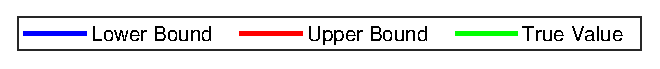
\includegraphics[scale=0.8]{figures/legend}\\\\
\begin{subfigure}{.5\linewidth}
\centering
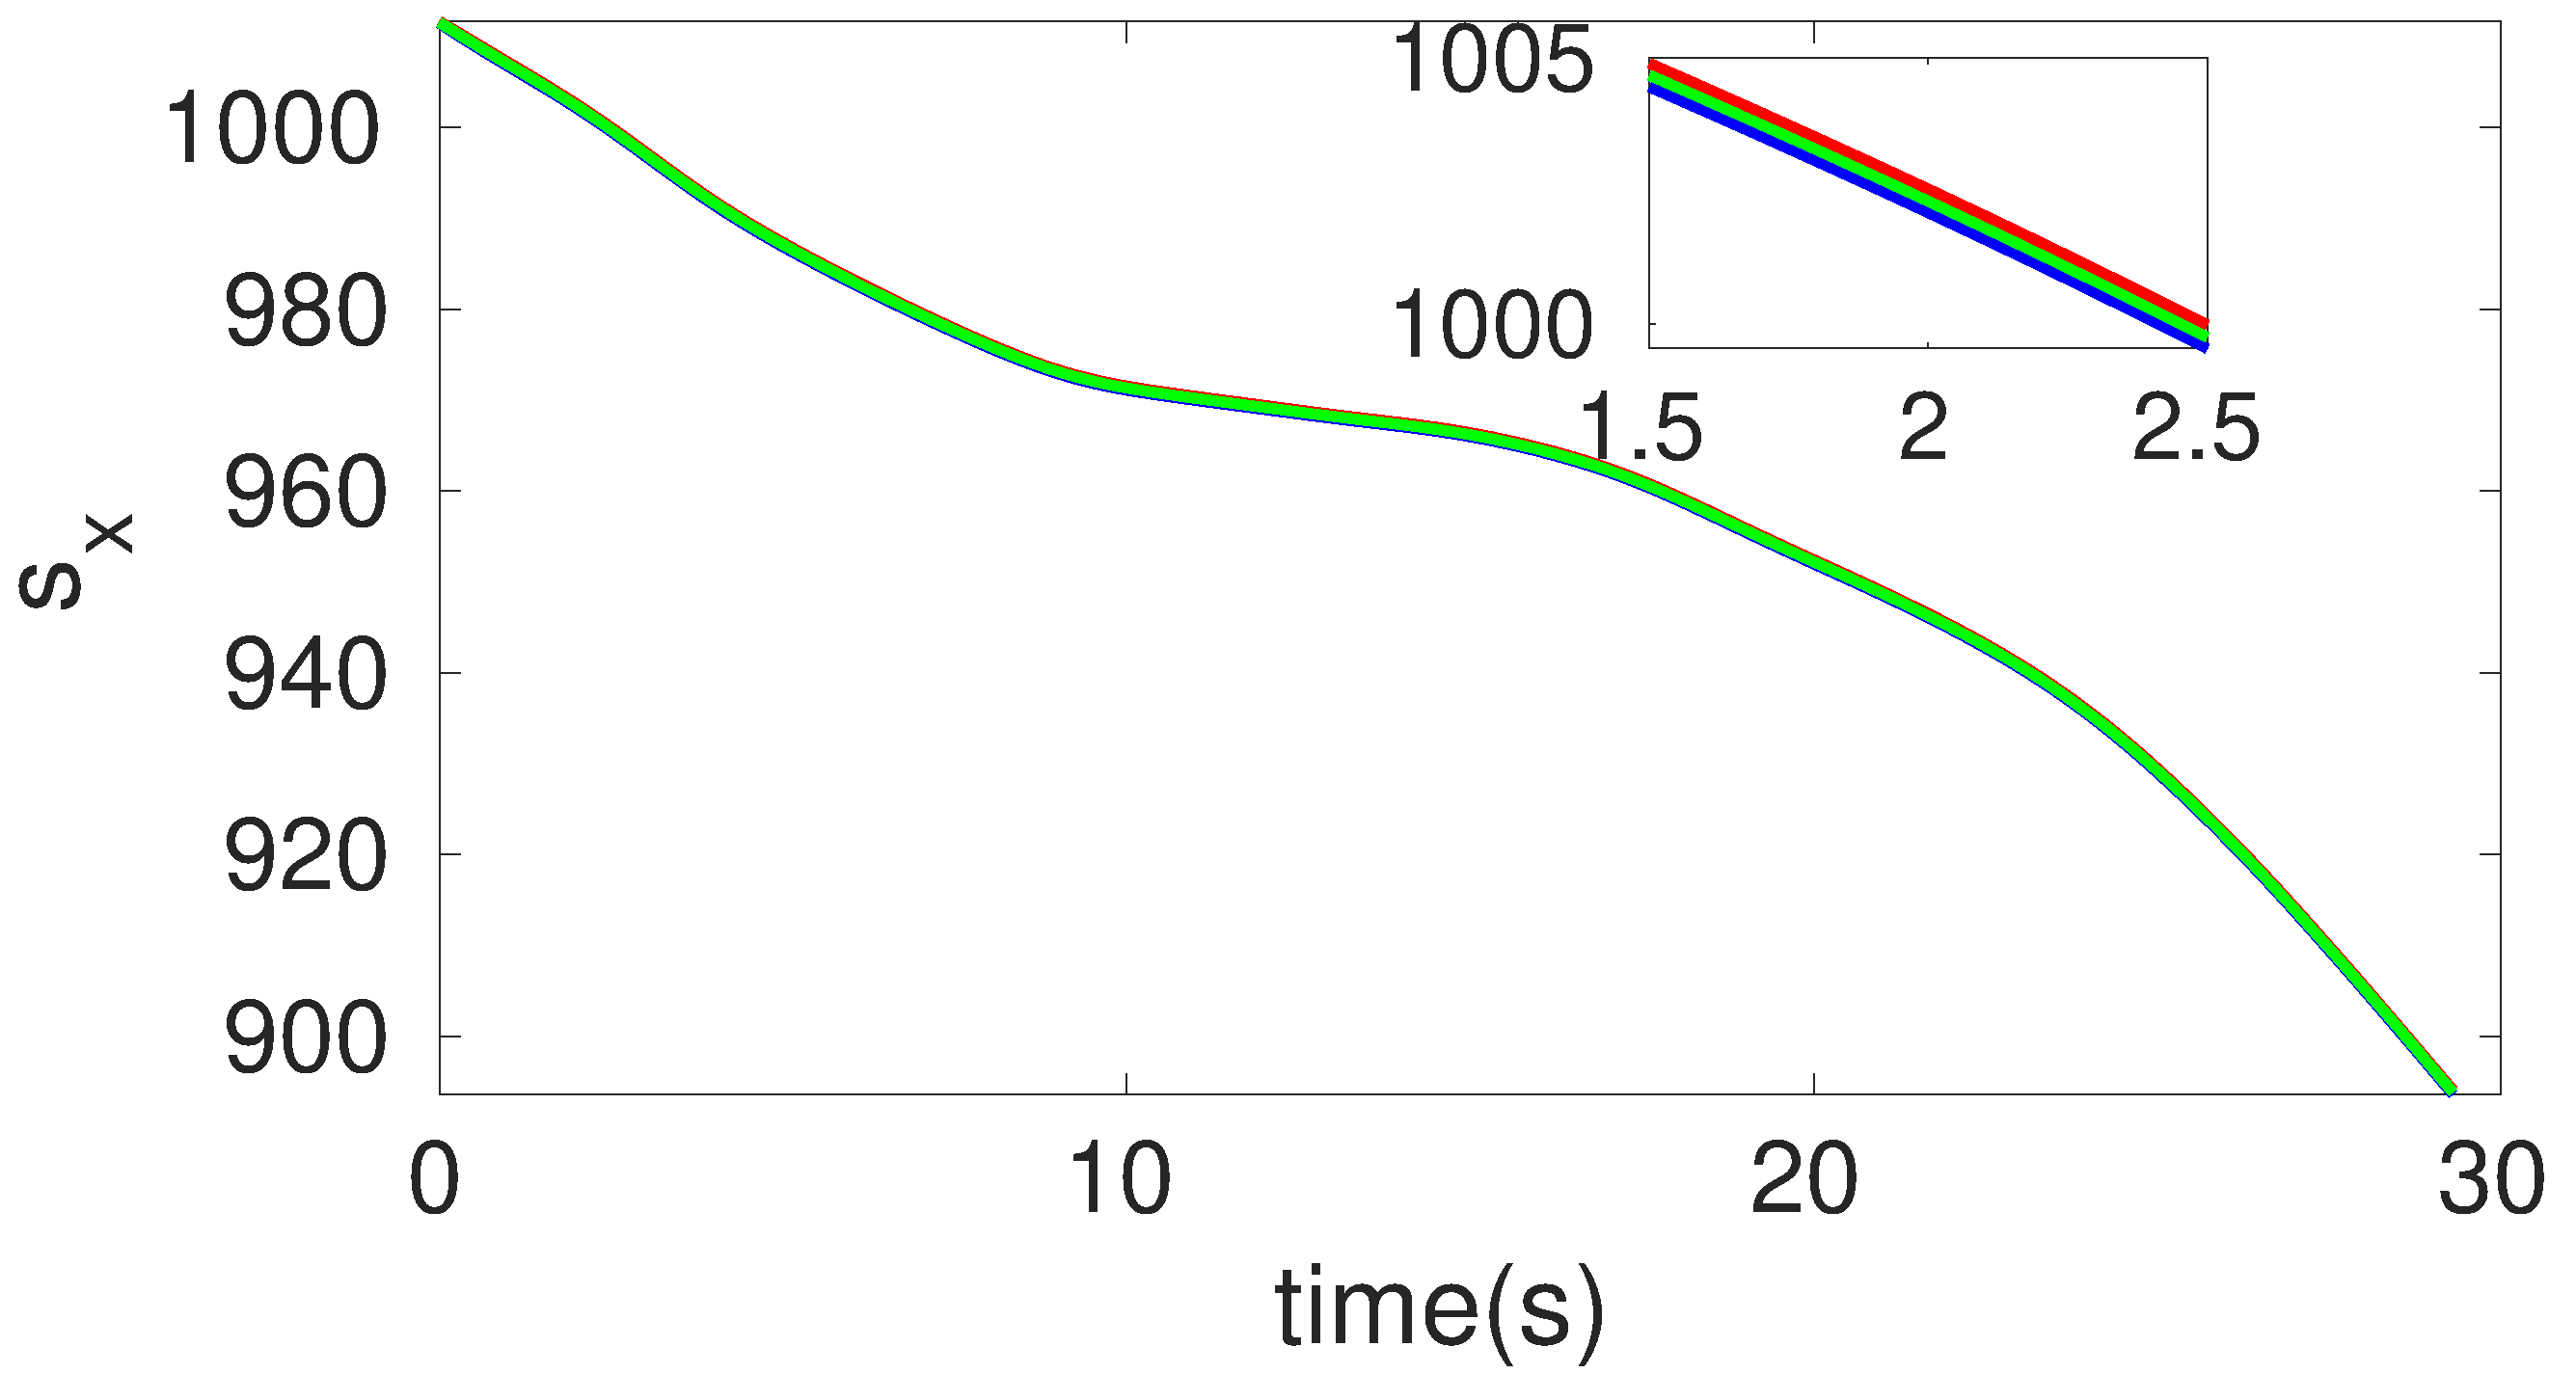
\includegraphics[width=\linewidth]{figures/Frad/s3cvSMs_x}
\end{subfigure}
\begin{subfigure}{.5\linewidth}
\centering
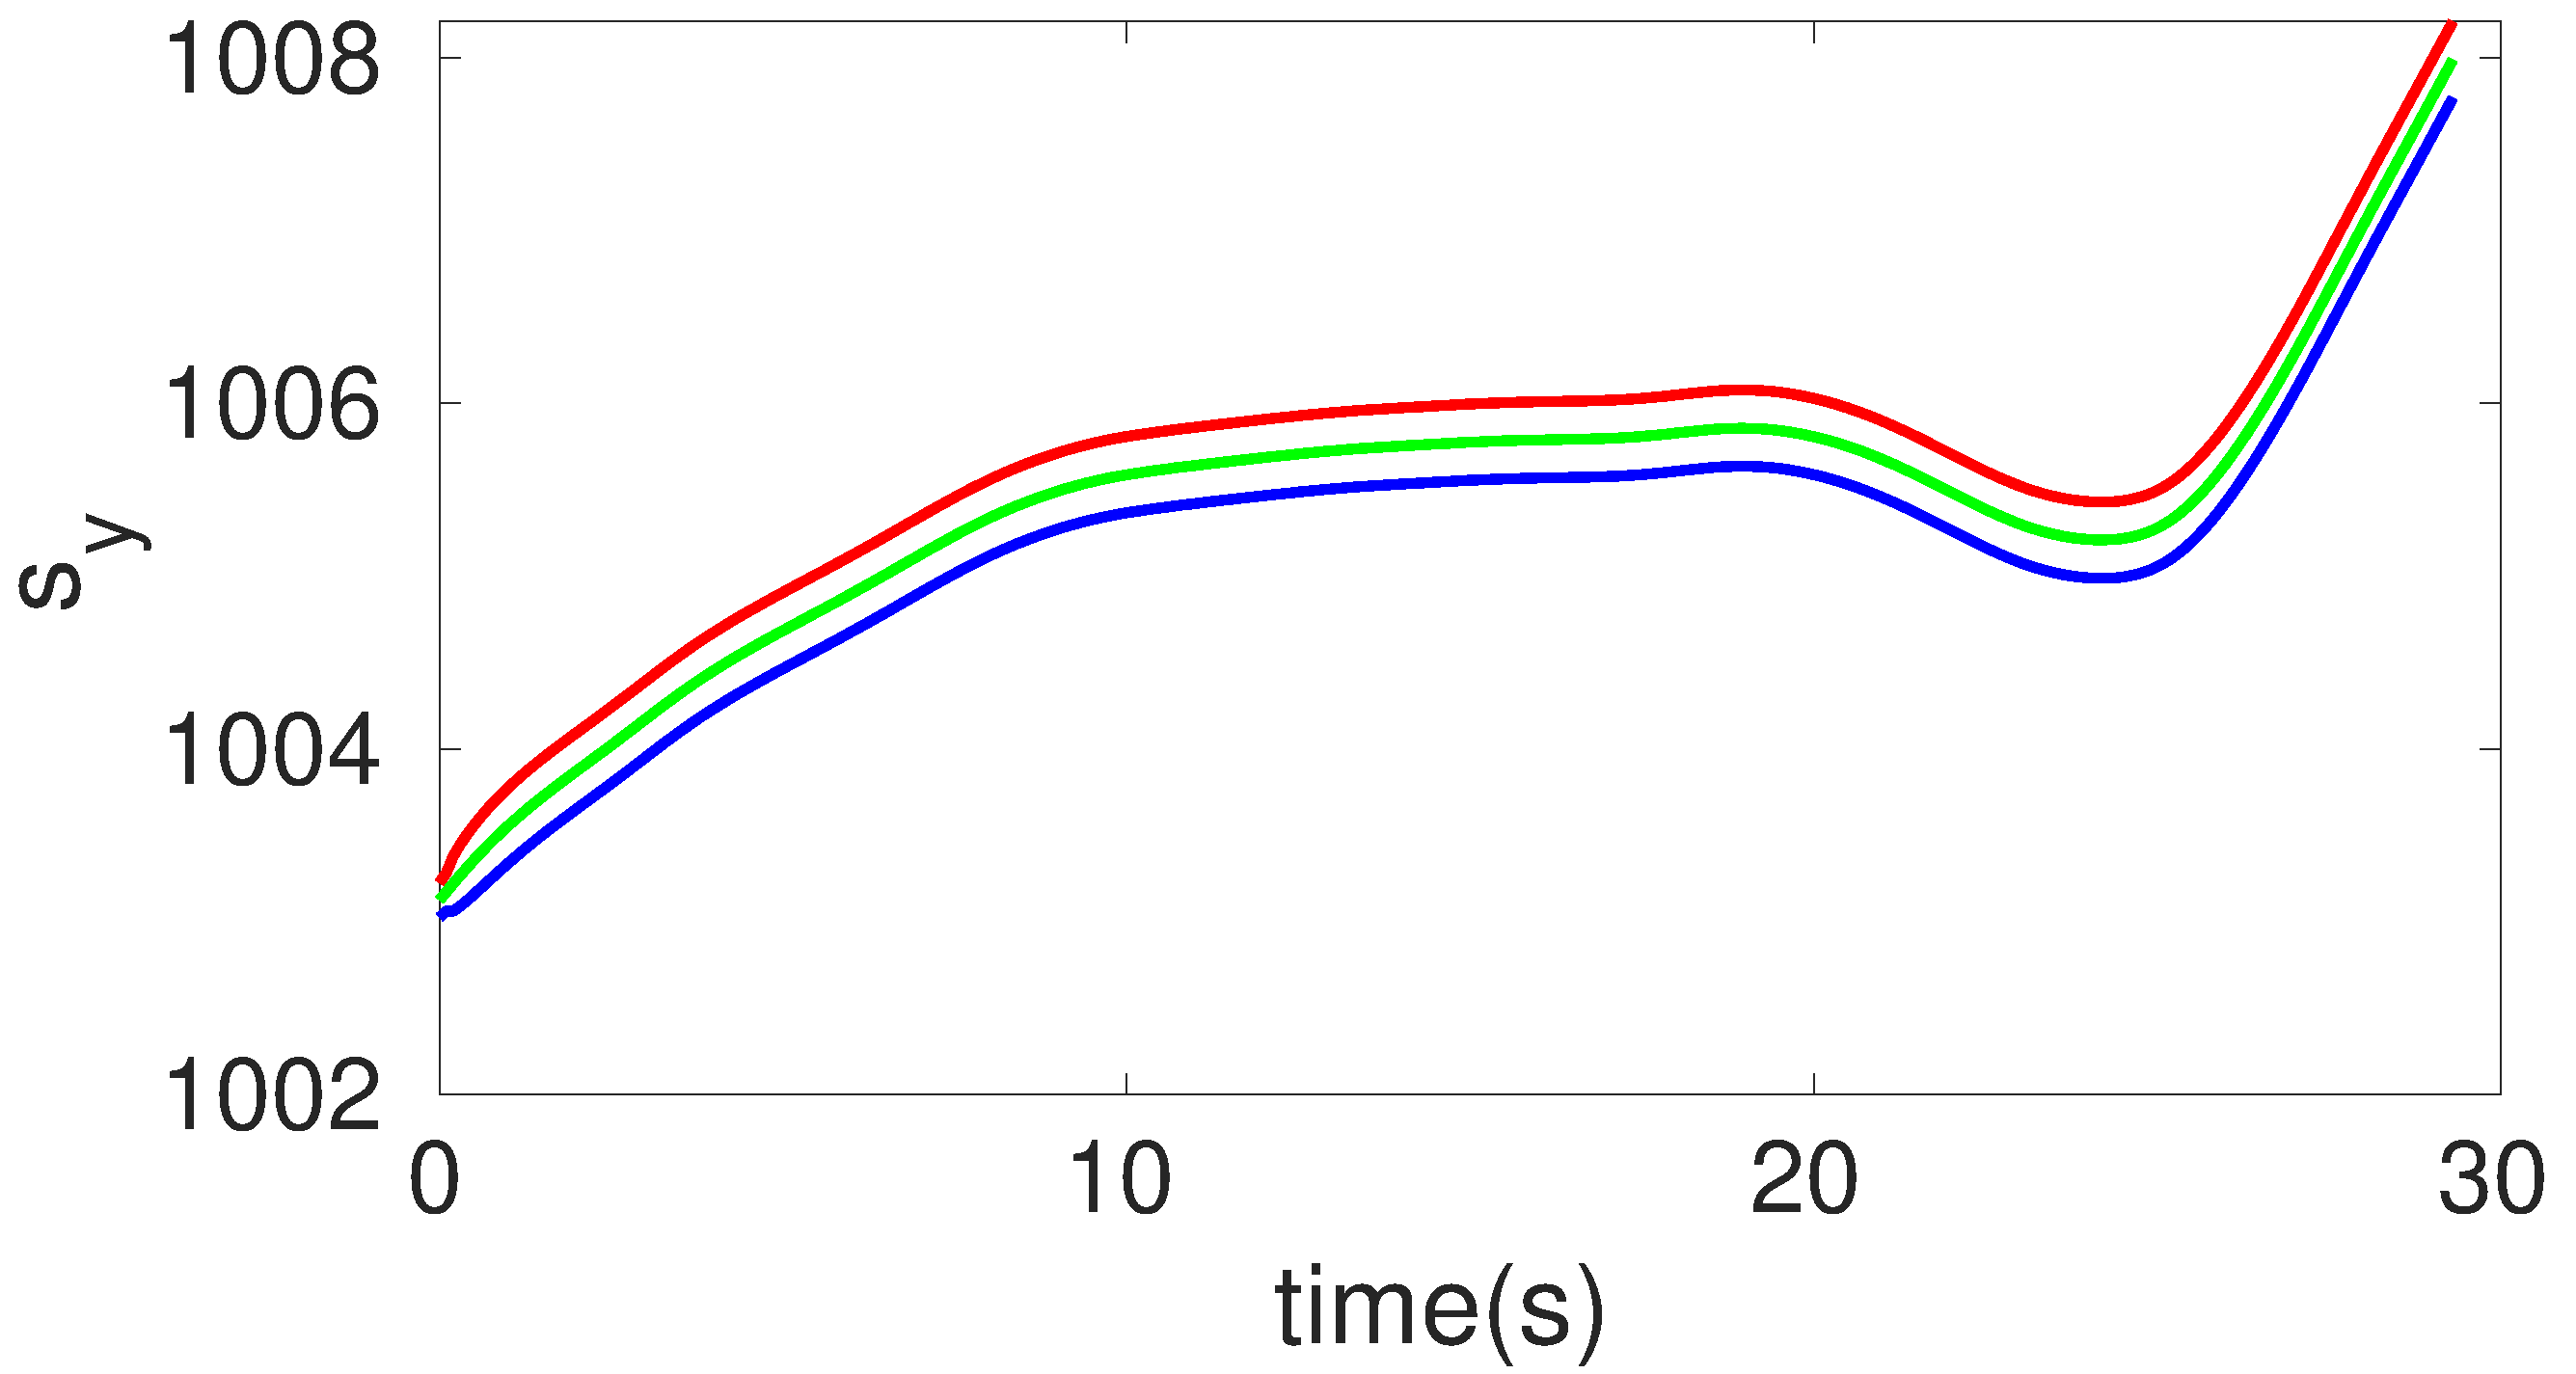
\includegraphics[width=\linewidth]{figures/Frad/s3cvSMs_y}
\end{subfigure}
\begin{subfigure}{.5\linewidth}
\centering
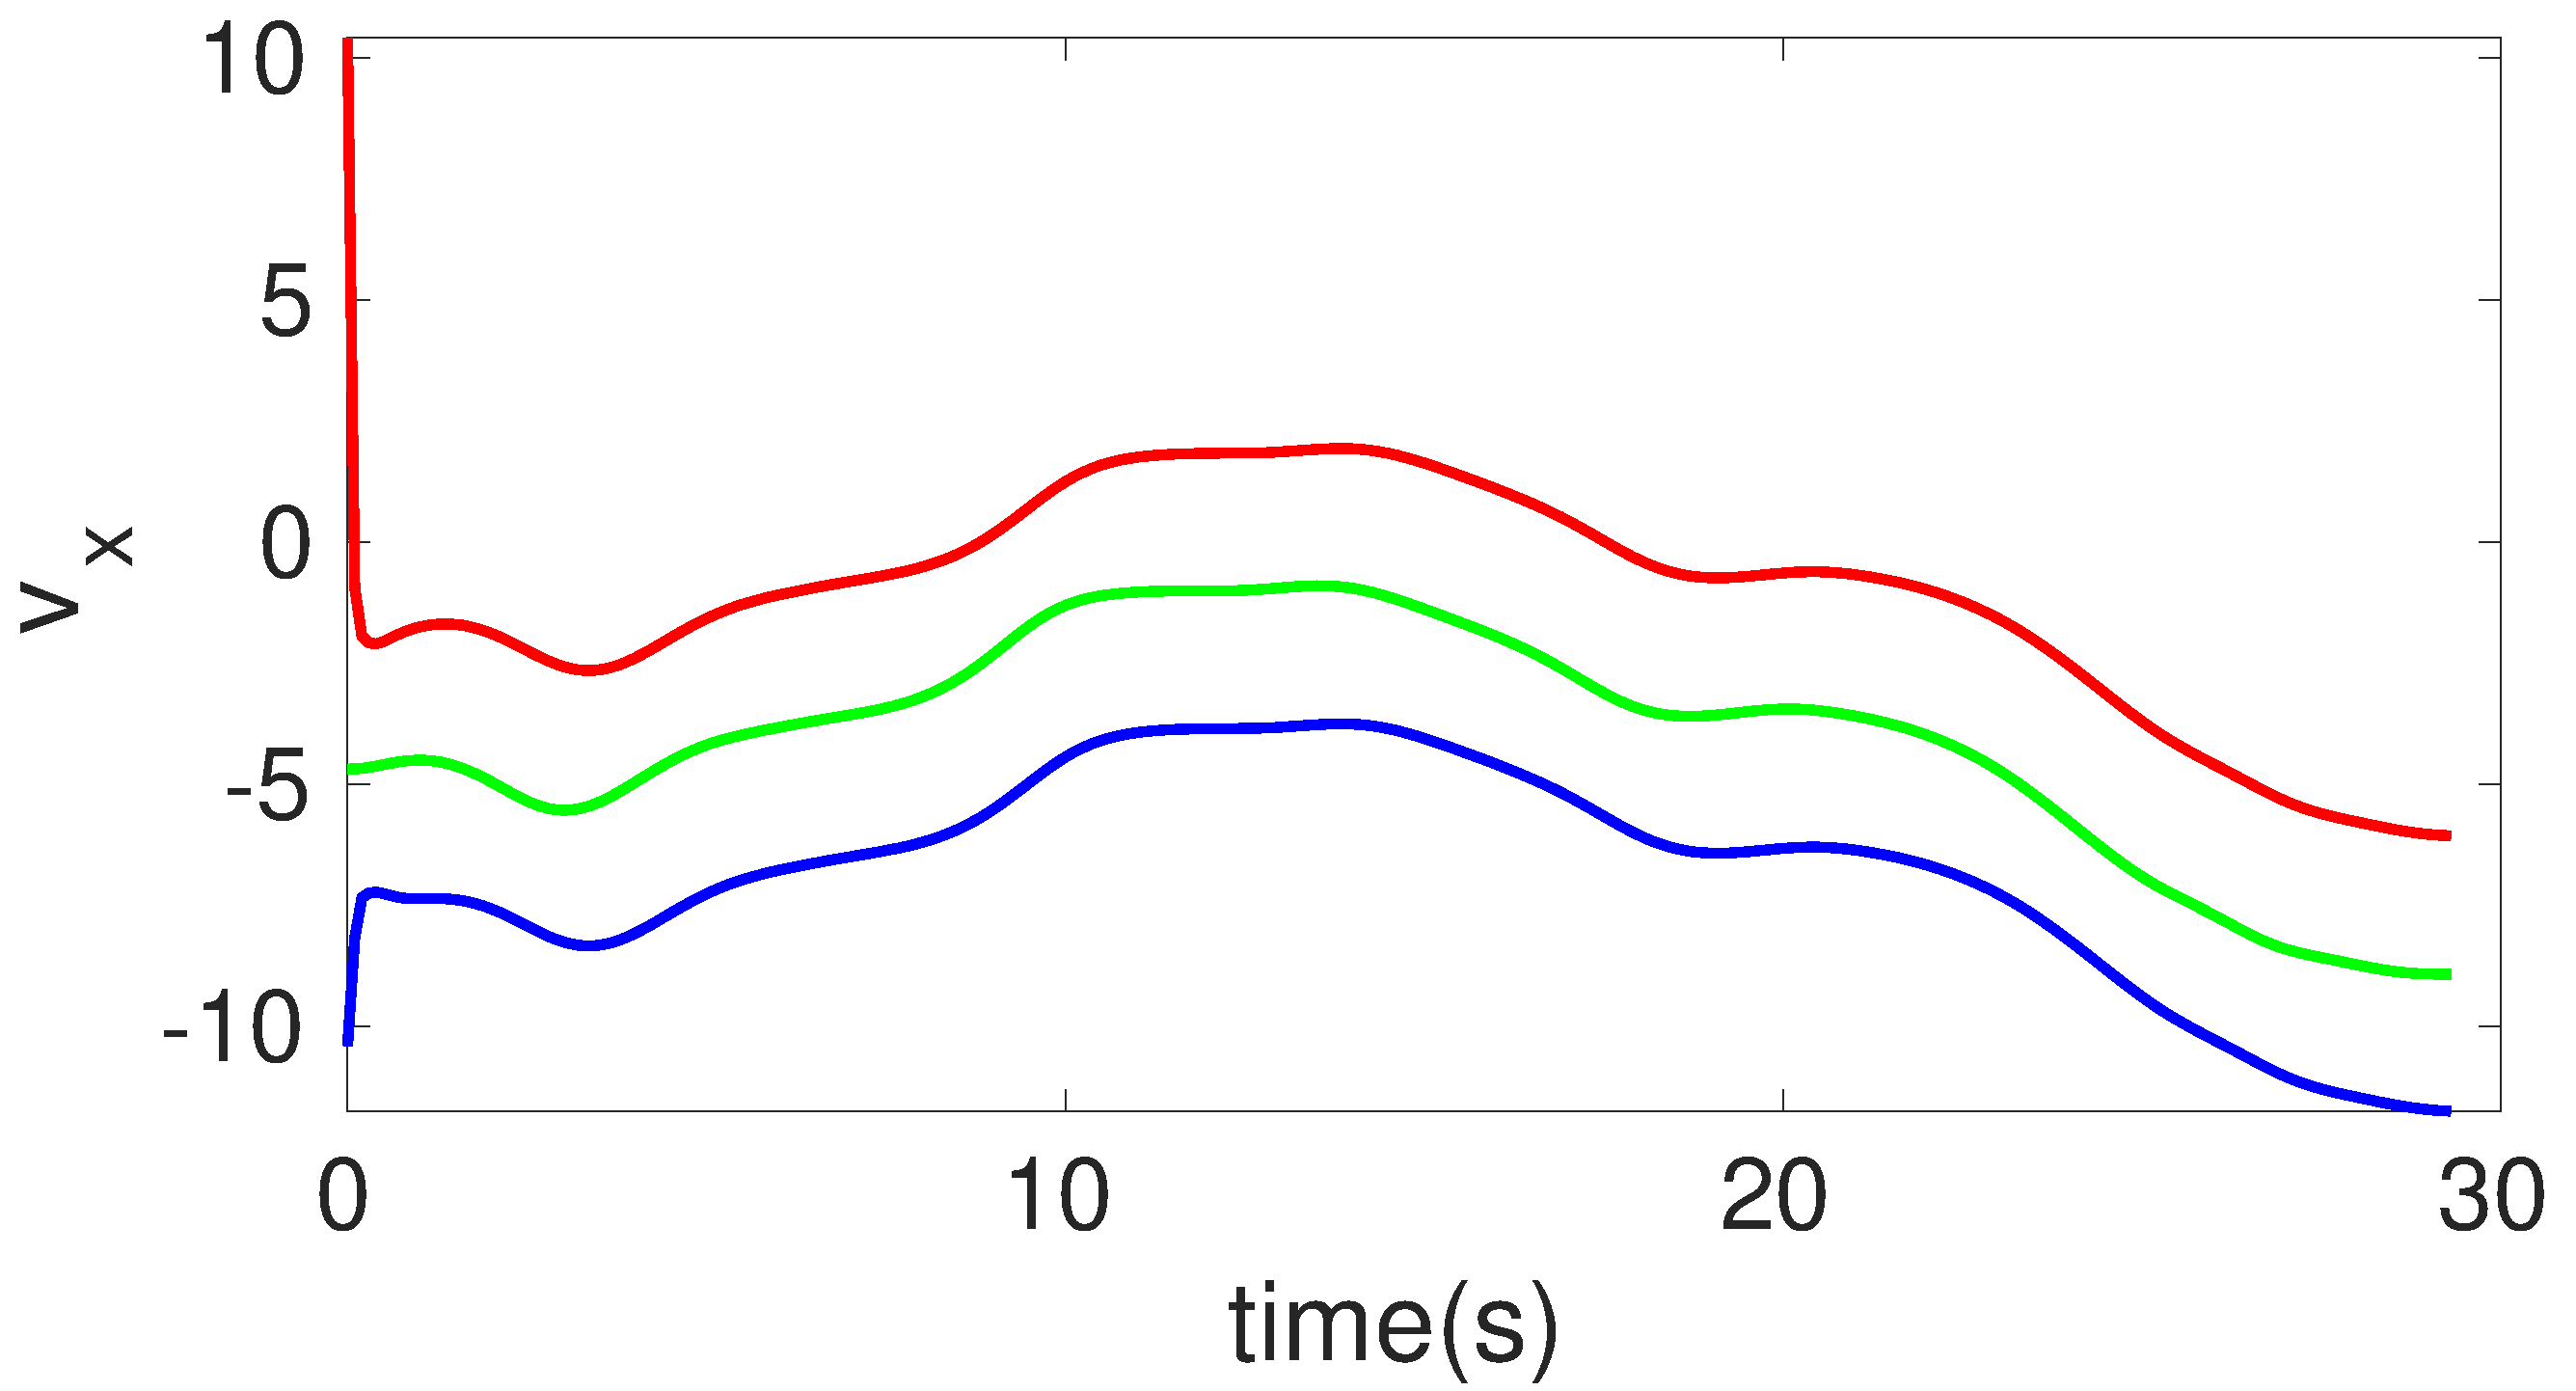
\includegraphics[width=\linewidth]{figures/Frad/s3cvSMv_x}
\end{subfigure}
\begin{subfigure}{.5\linewidth}
\centering
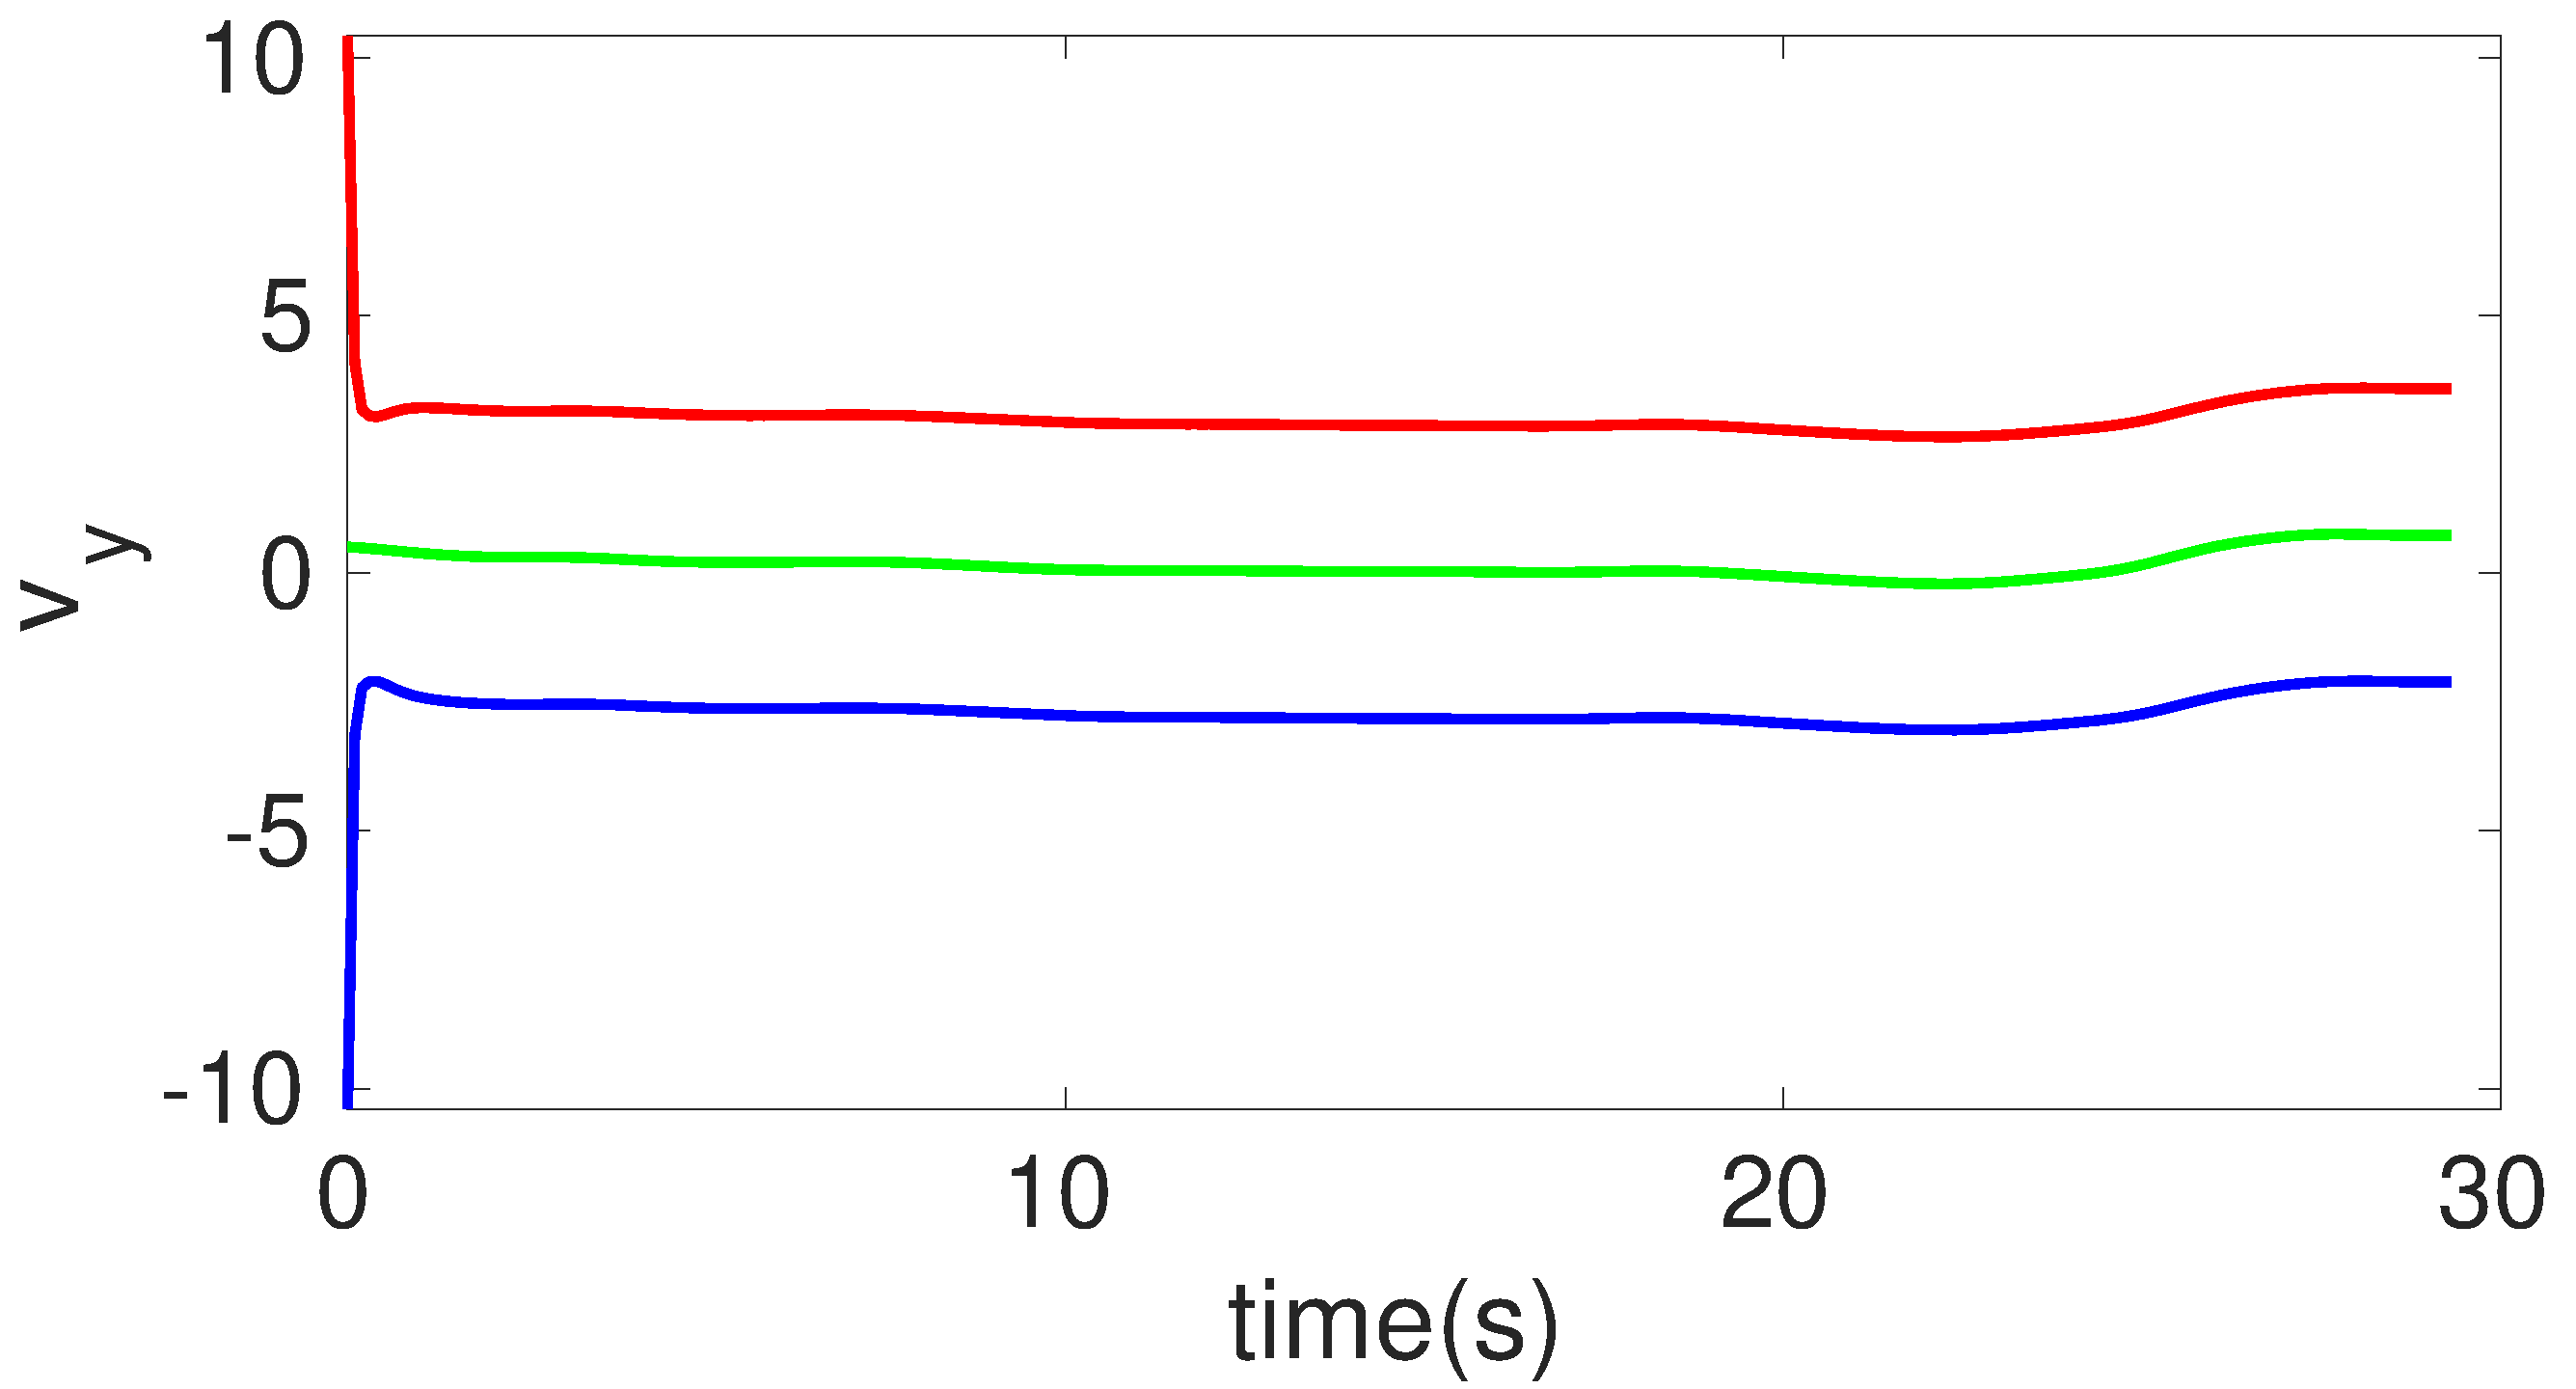
\includegraphics[width=\linewidth]{figures/Frad/s3cvSMv_y}
\end{subfigure}
\caption{Estimation using the F-radius minimizer and the constant velocity model}
\end{figure}

\begin{figure}[h]
\hspace*{\fill} 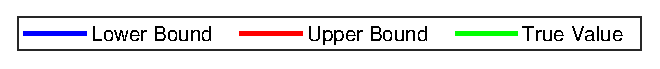
\includegraphics[scale=0.8]{figures/legend}\\\\
\begin{subfigure}{.5\linewidth}
\centering
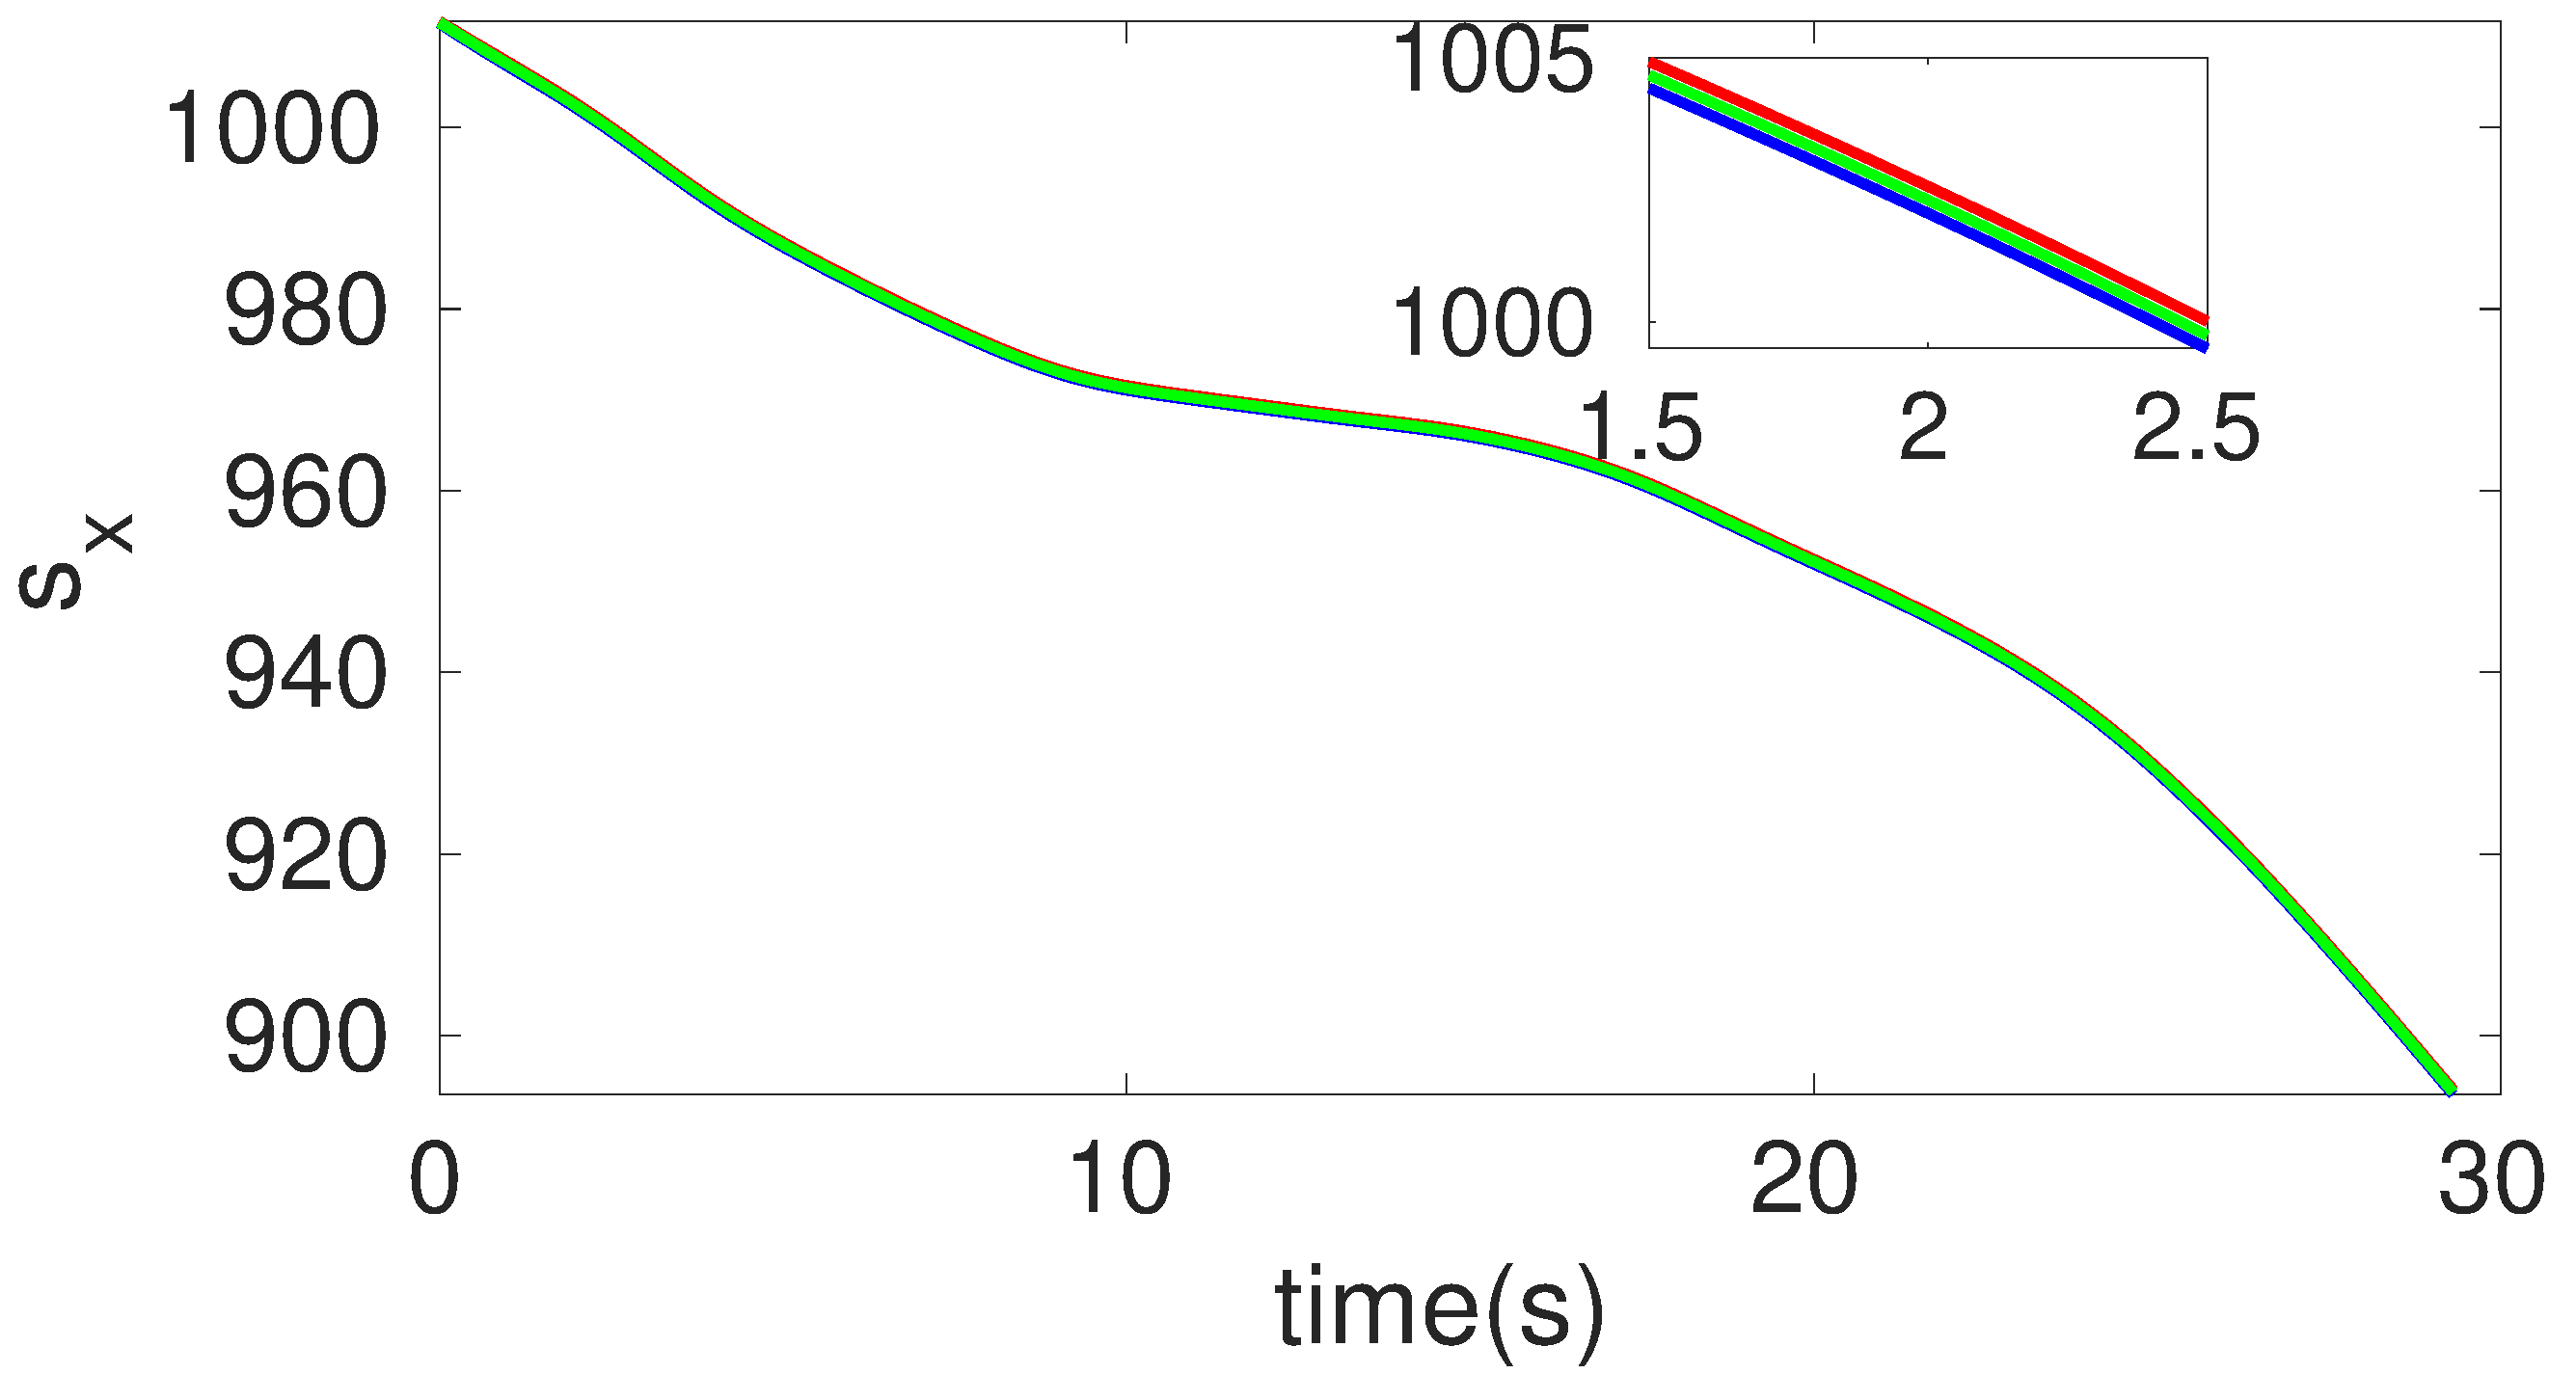
\includegraphics[width=\linewidth]{figures/Frad/s3caSMs_x}
\end{subfigure}
\begin{subfigure}{.5\linewidth}
\centering
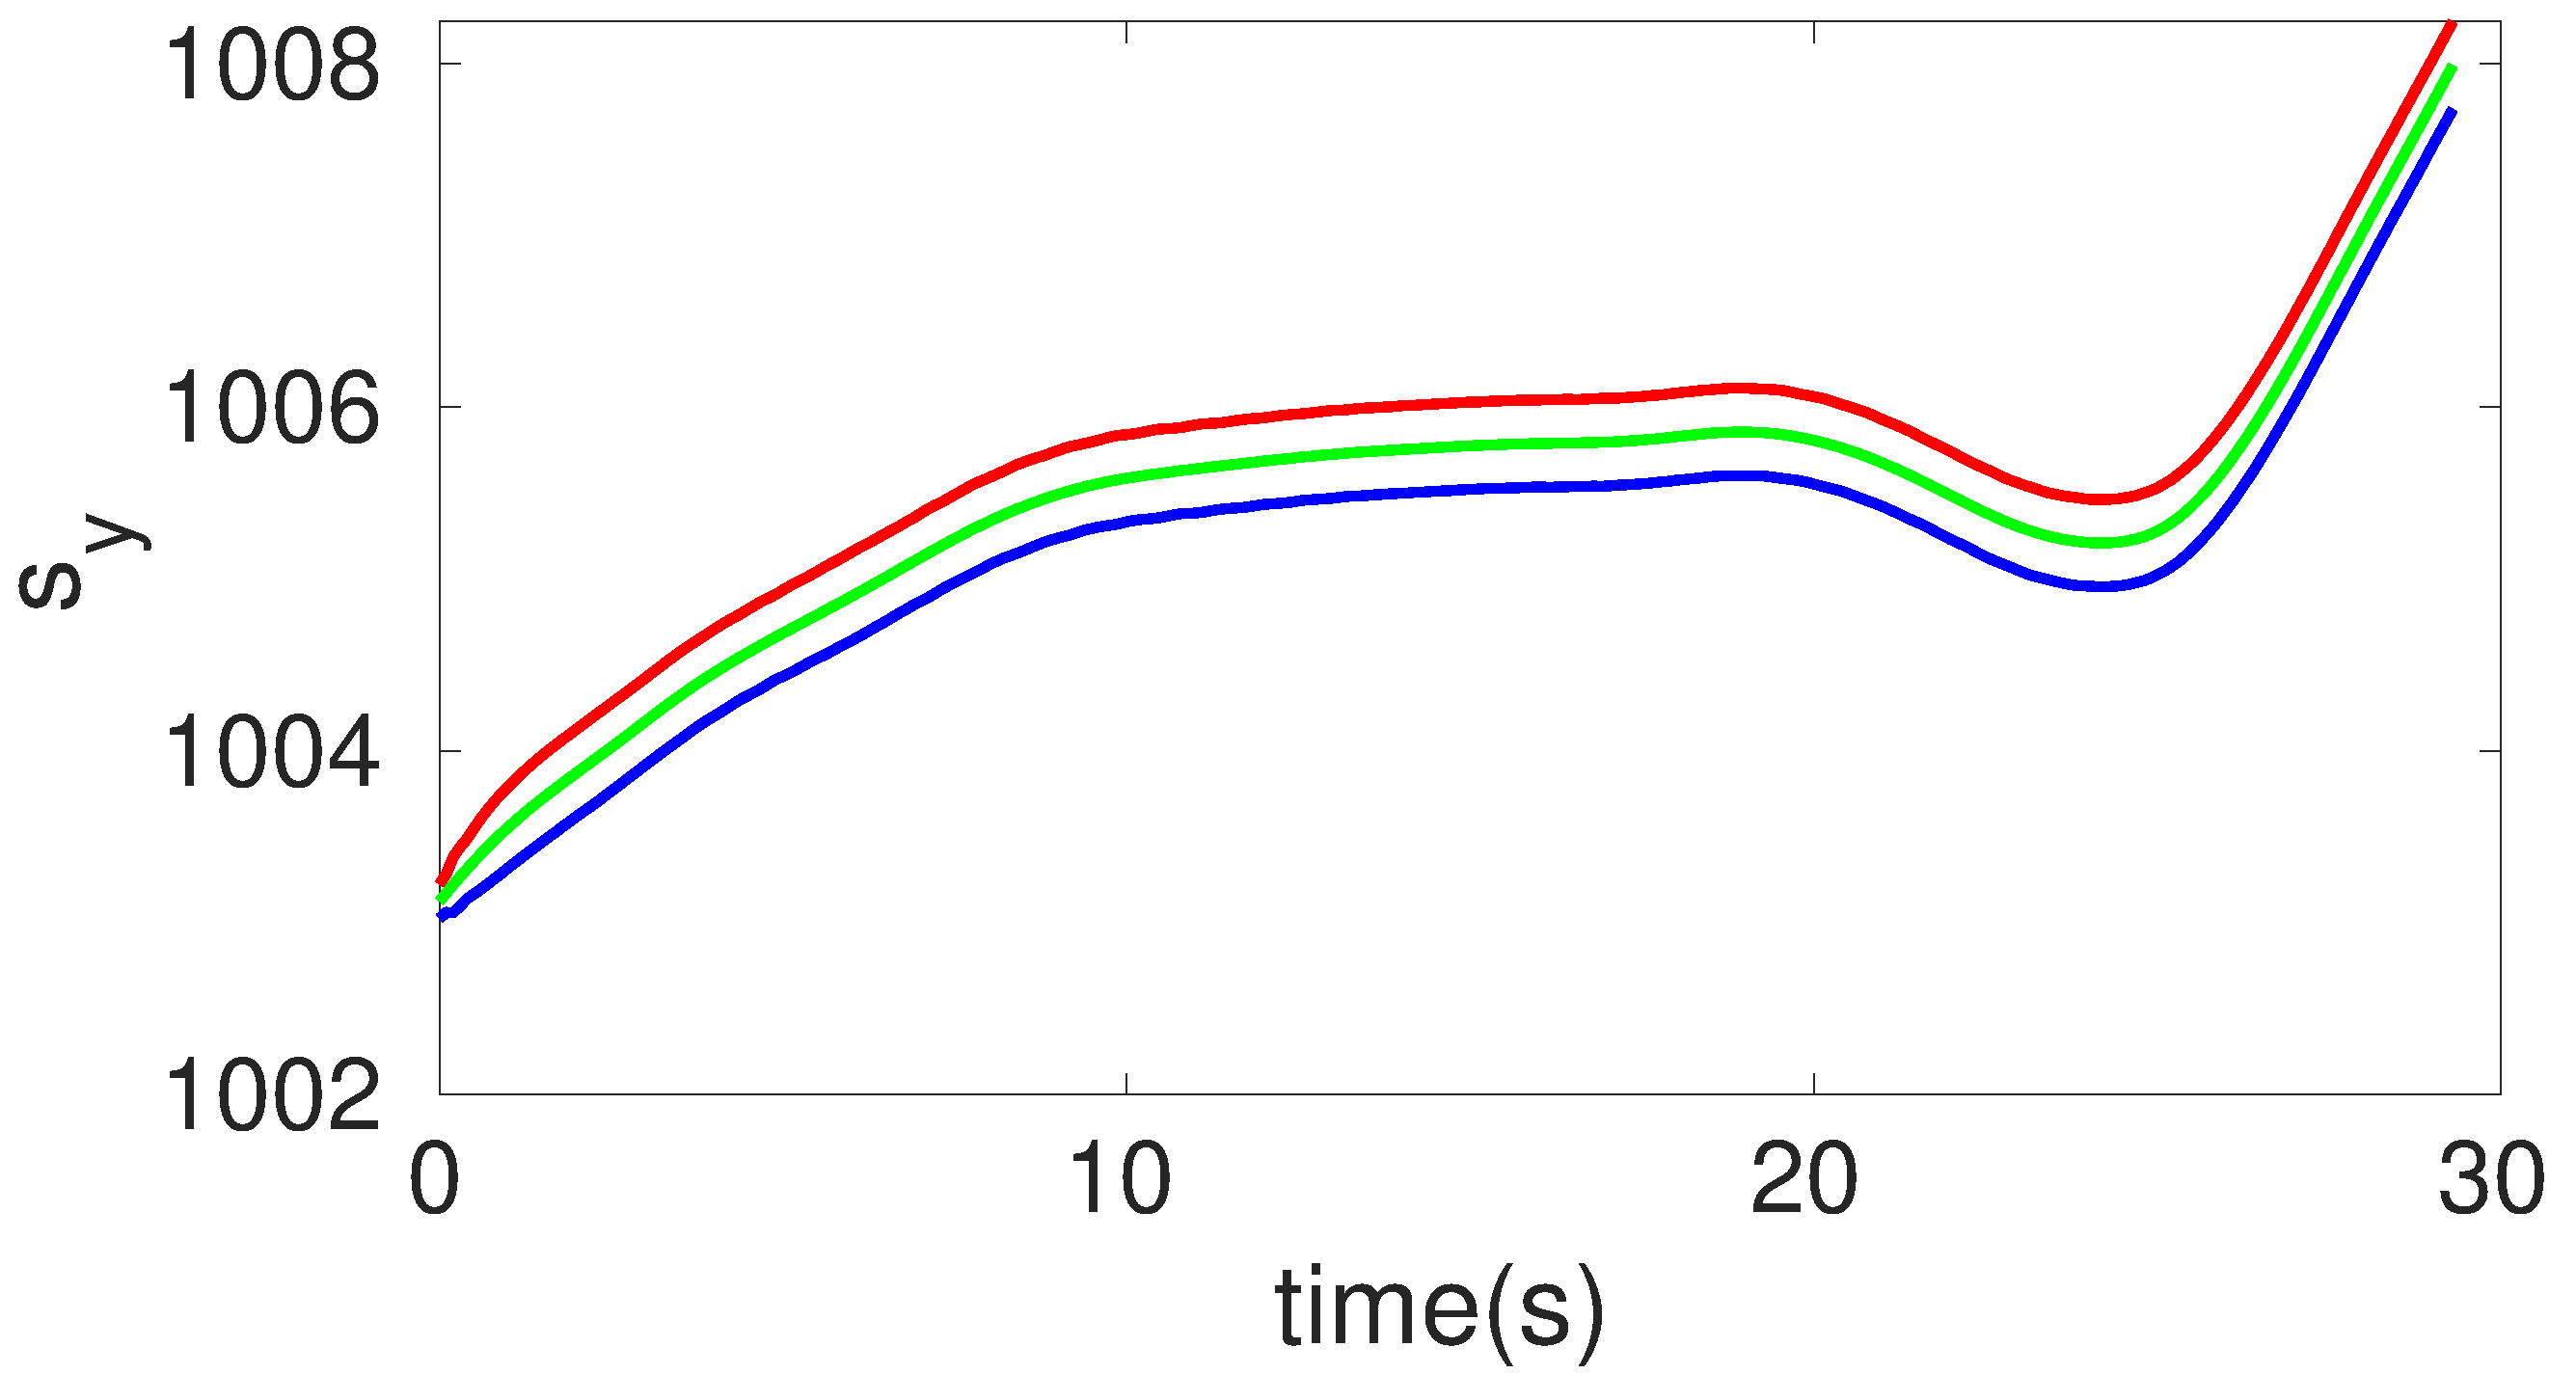
\includegraphics[width=\linewidth]{figures/Frad/s3caSMs_y}
\end{subfigure}
\begin{subfigure}{.5\linewidth}
\centering
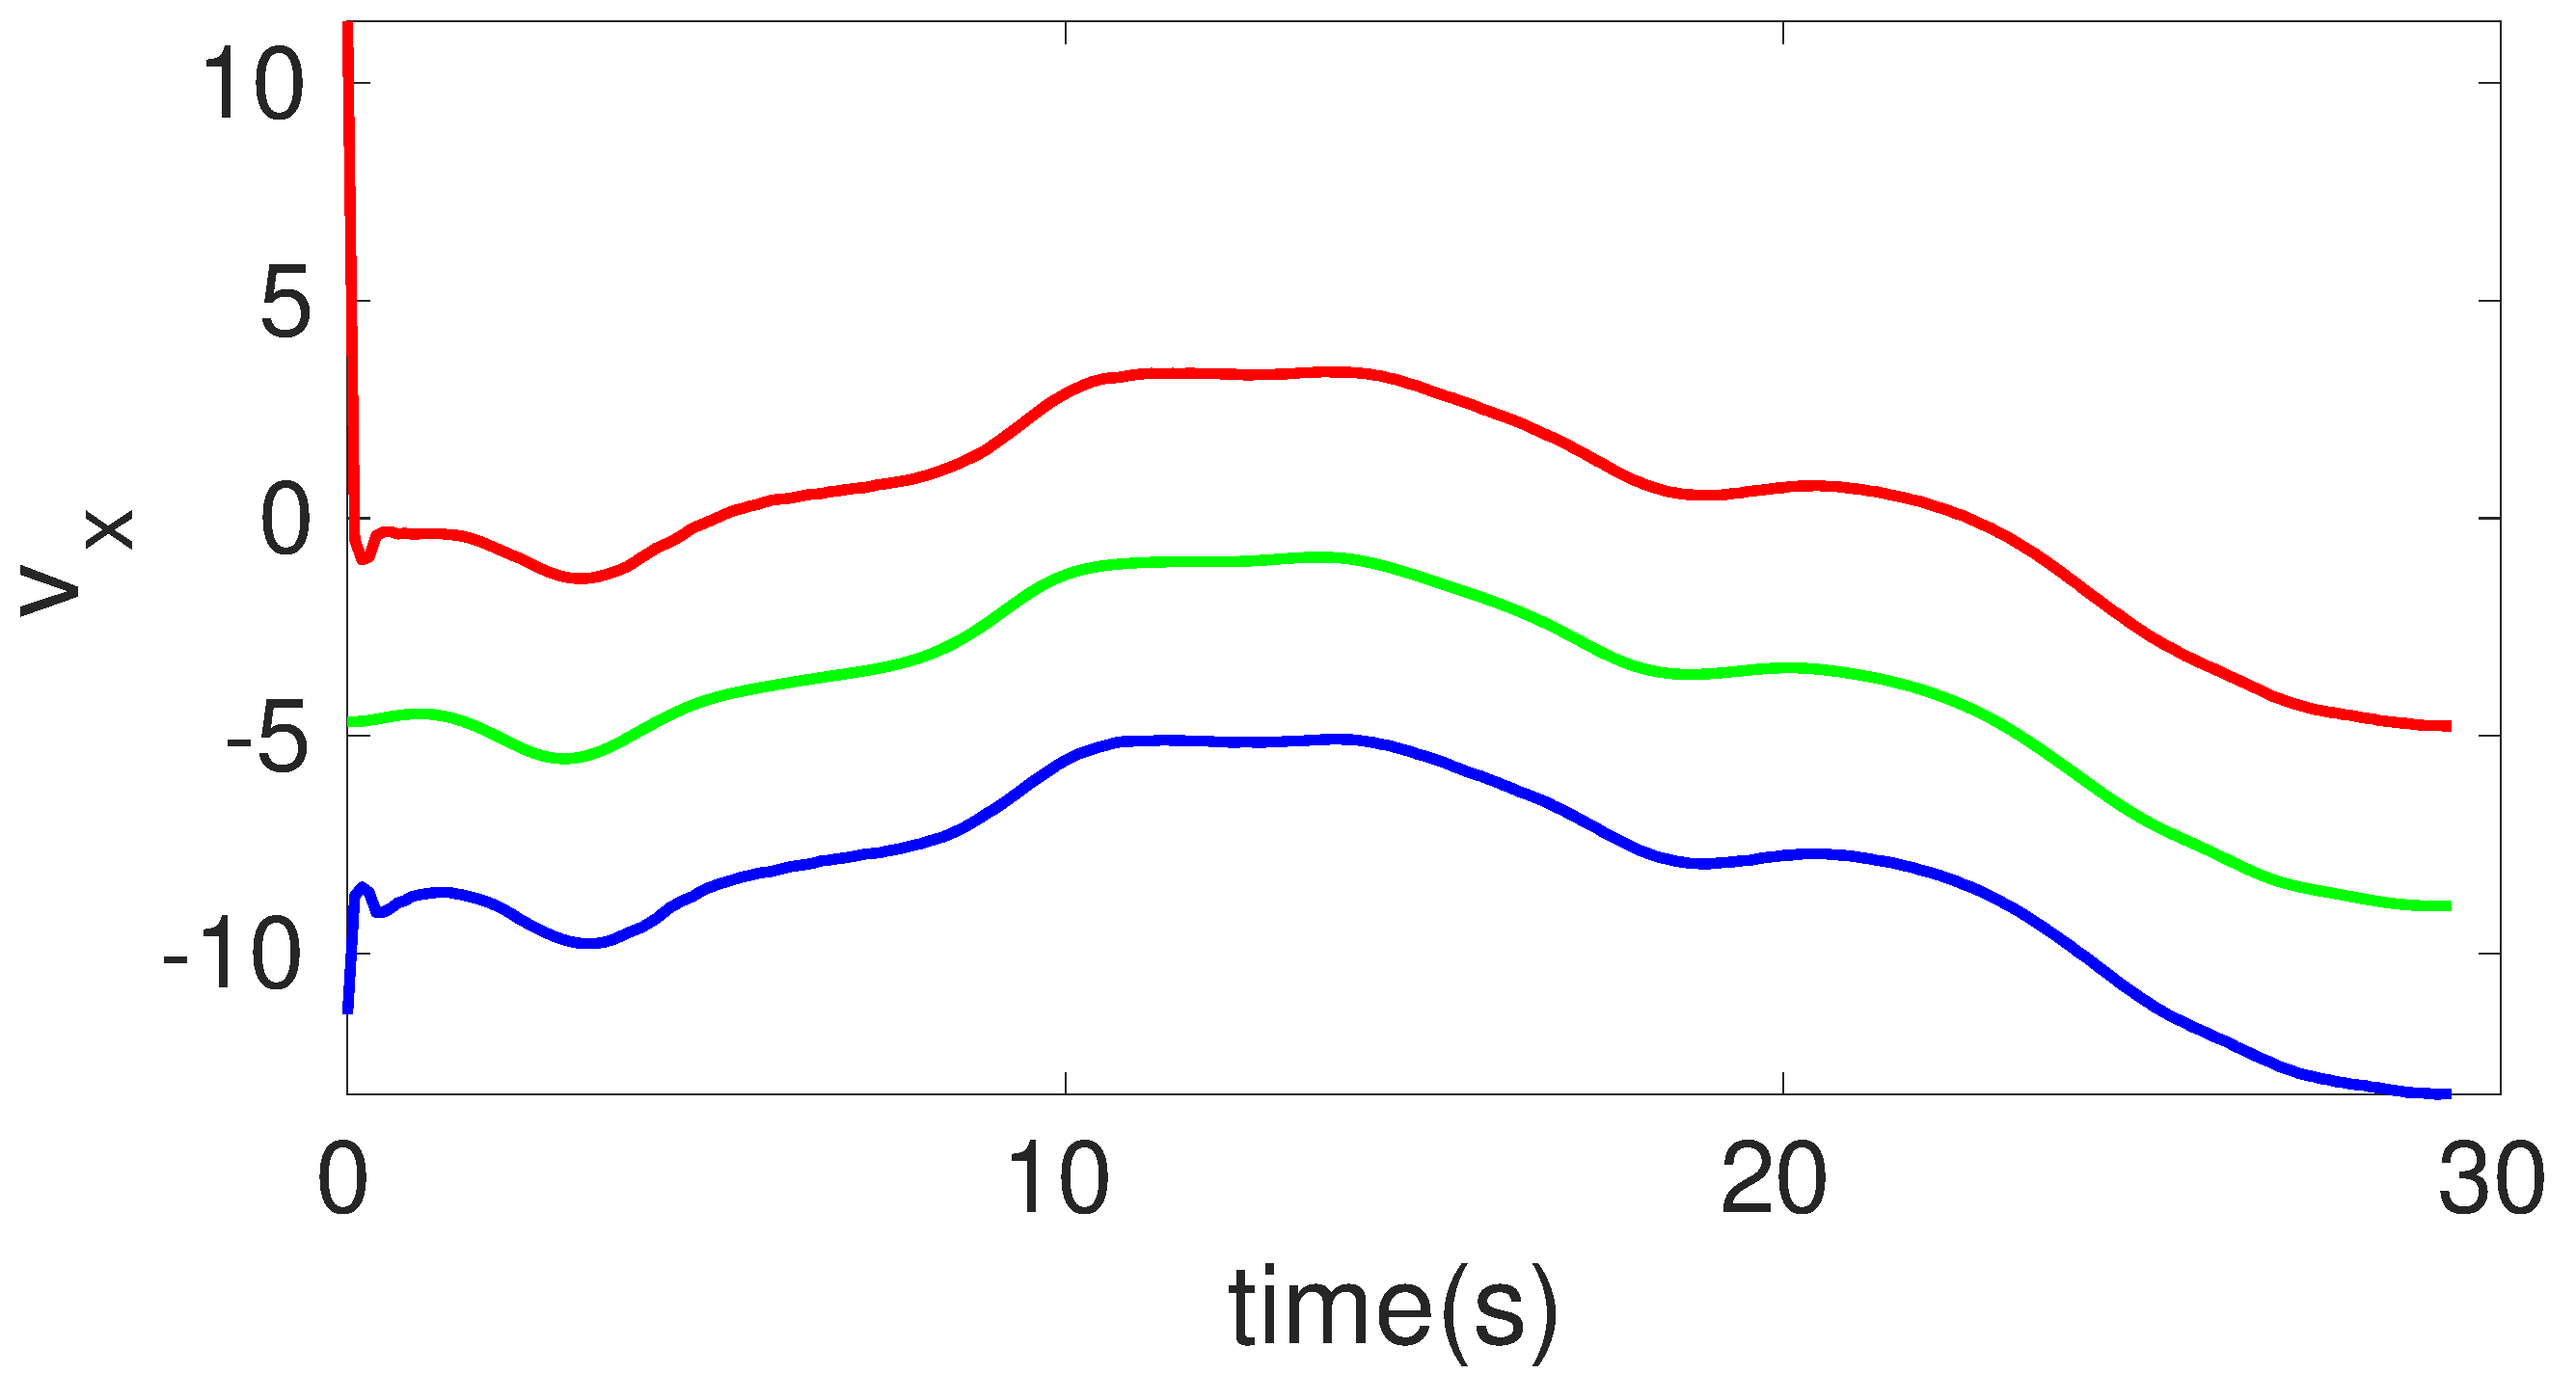
\includegraphics[width=\linewidth]{figures/Frad/s3caSMv_x}
\end{subfigure}
\begin{subfigure}{.5\linewidth}
\centering
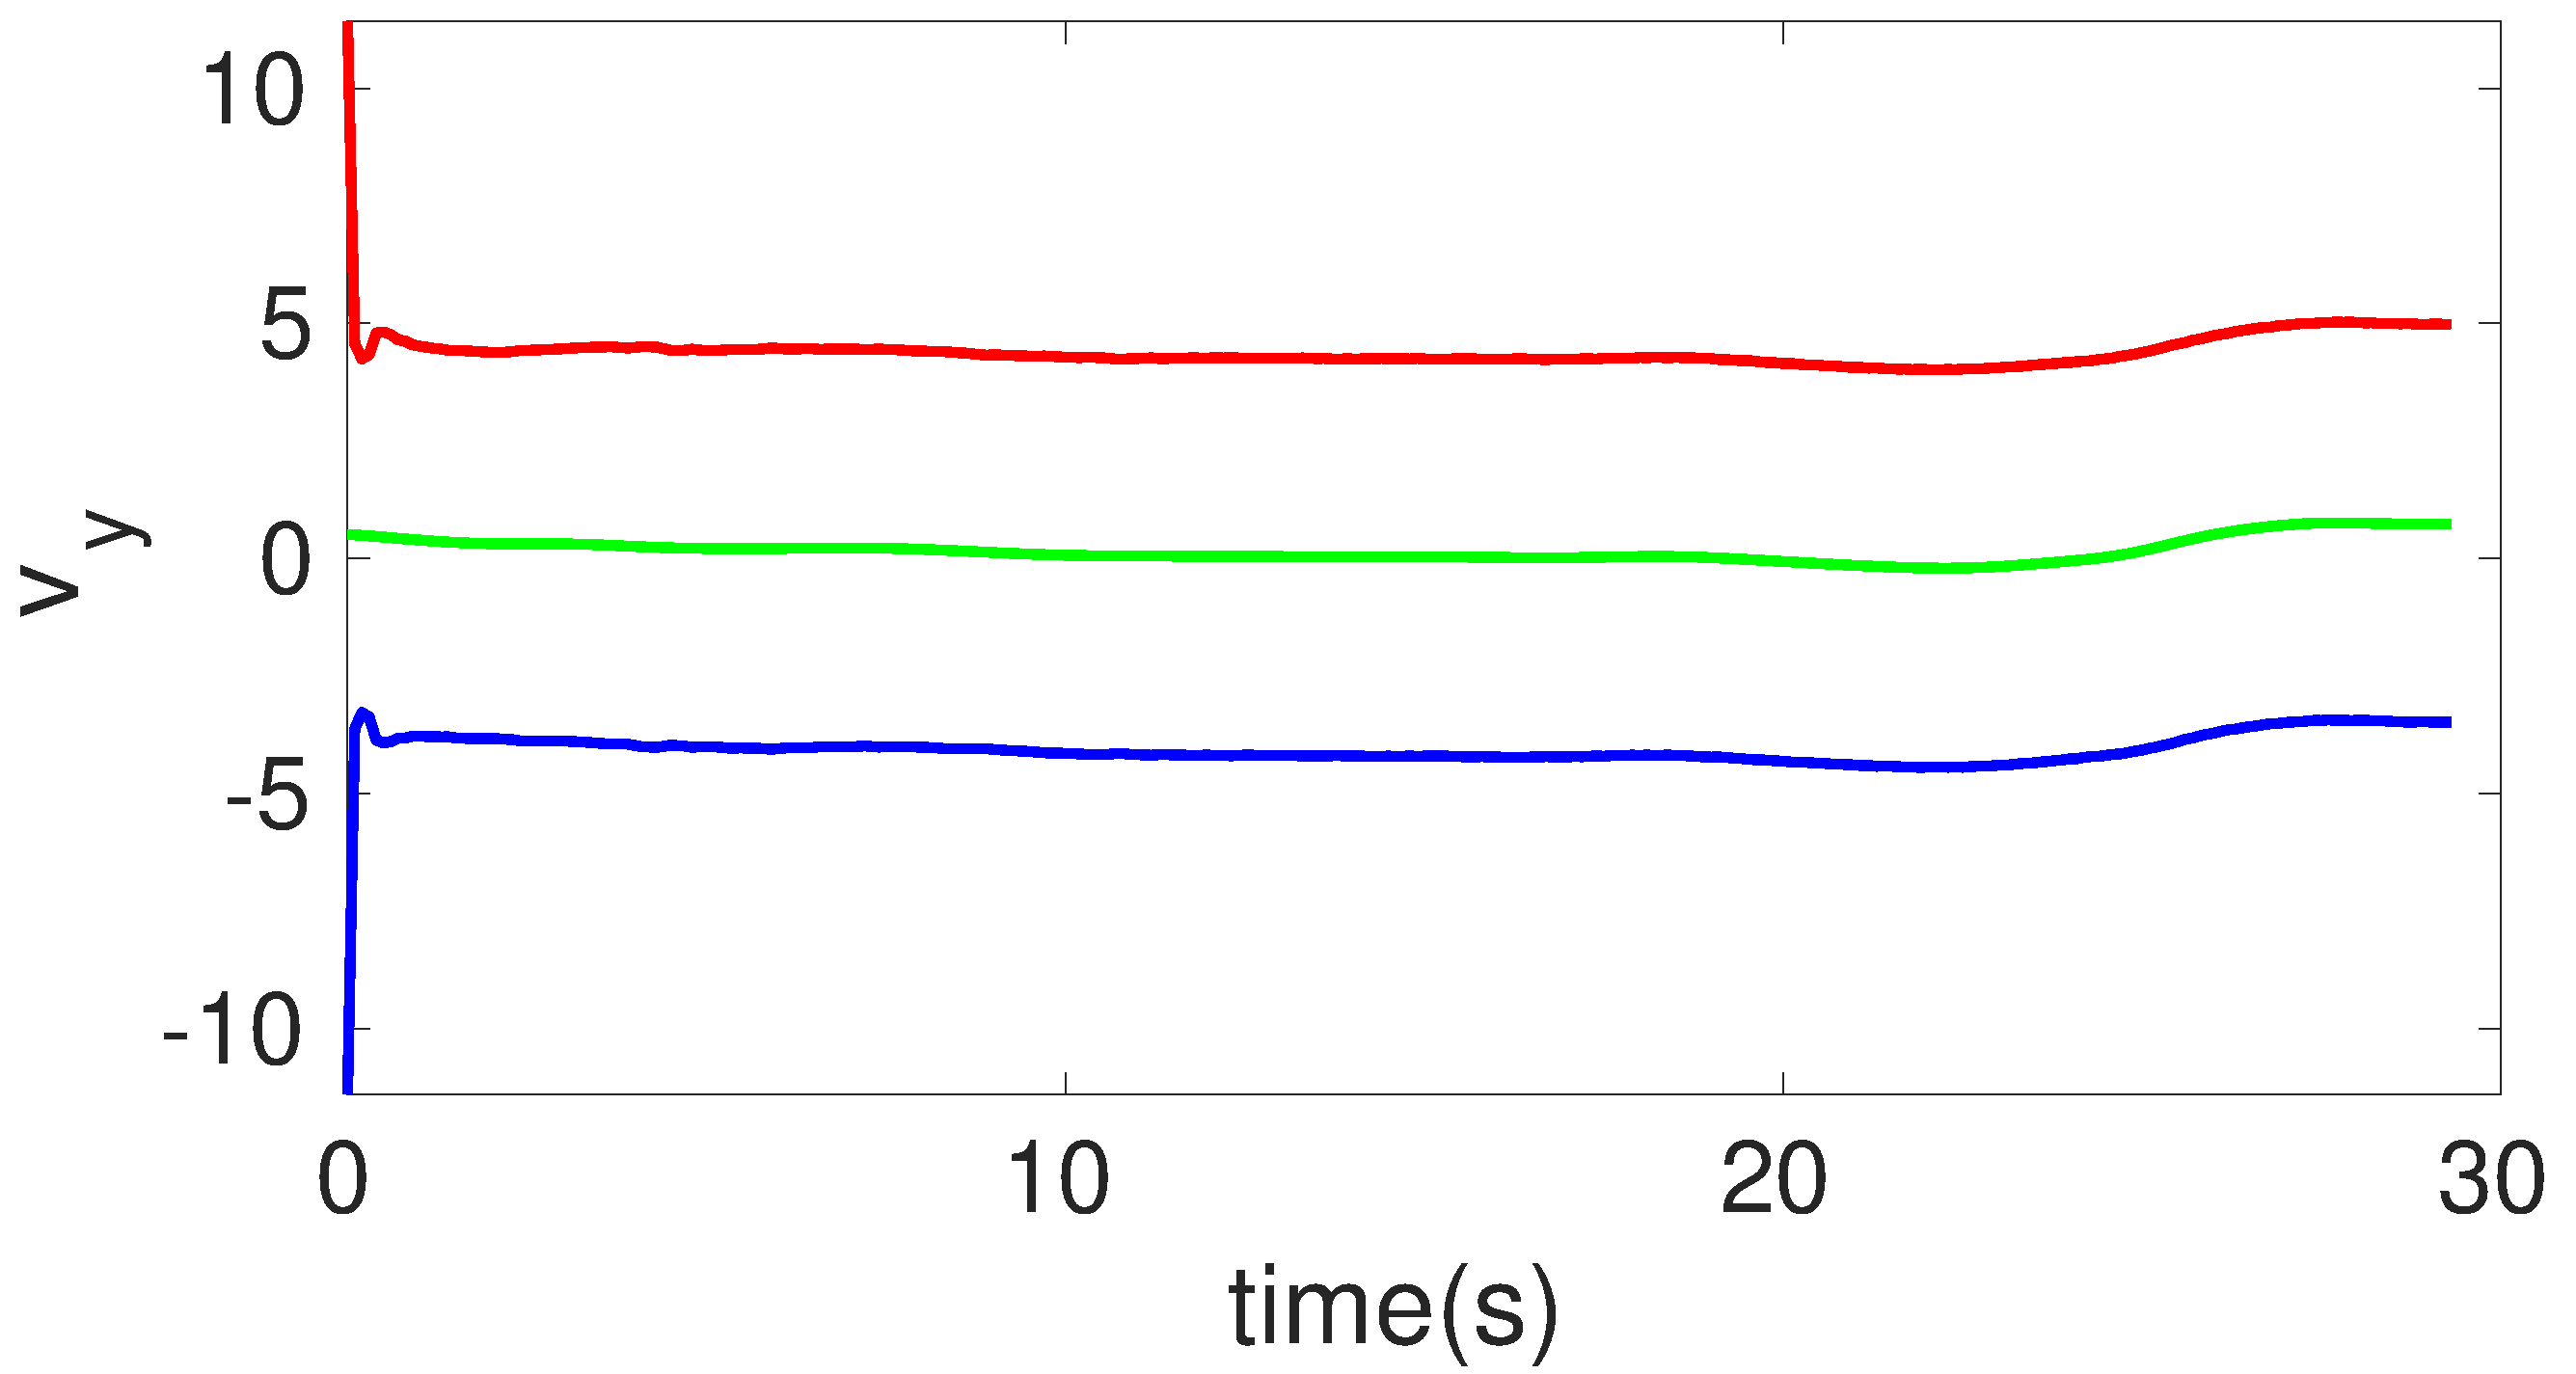
\includegraphics[width=\linewidth]{figures/Frad/s3caSMv_y}
\end{subfigure}
\begin{subfigure}{.5\linewidth}
\centering
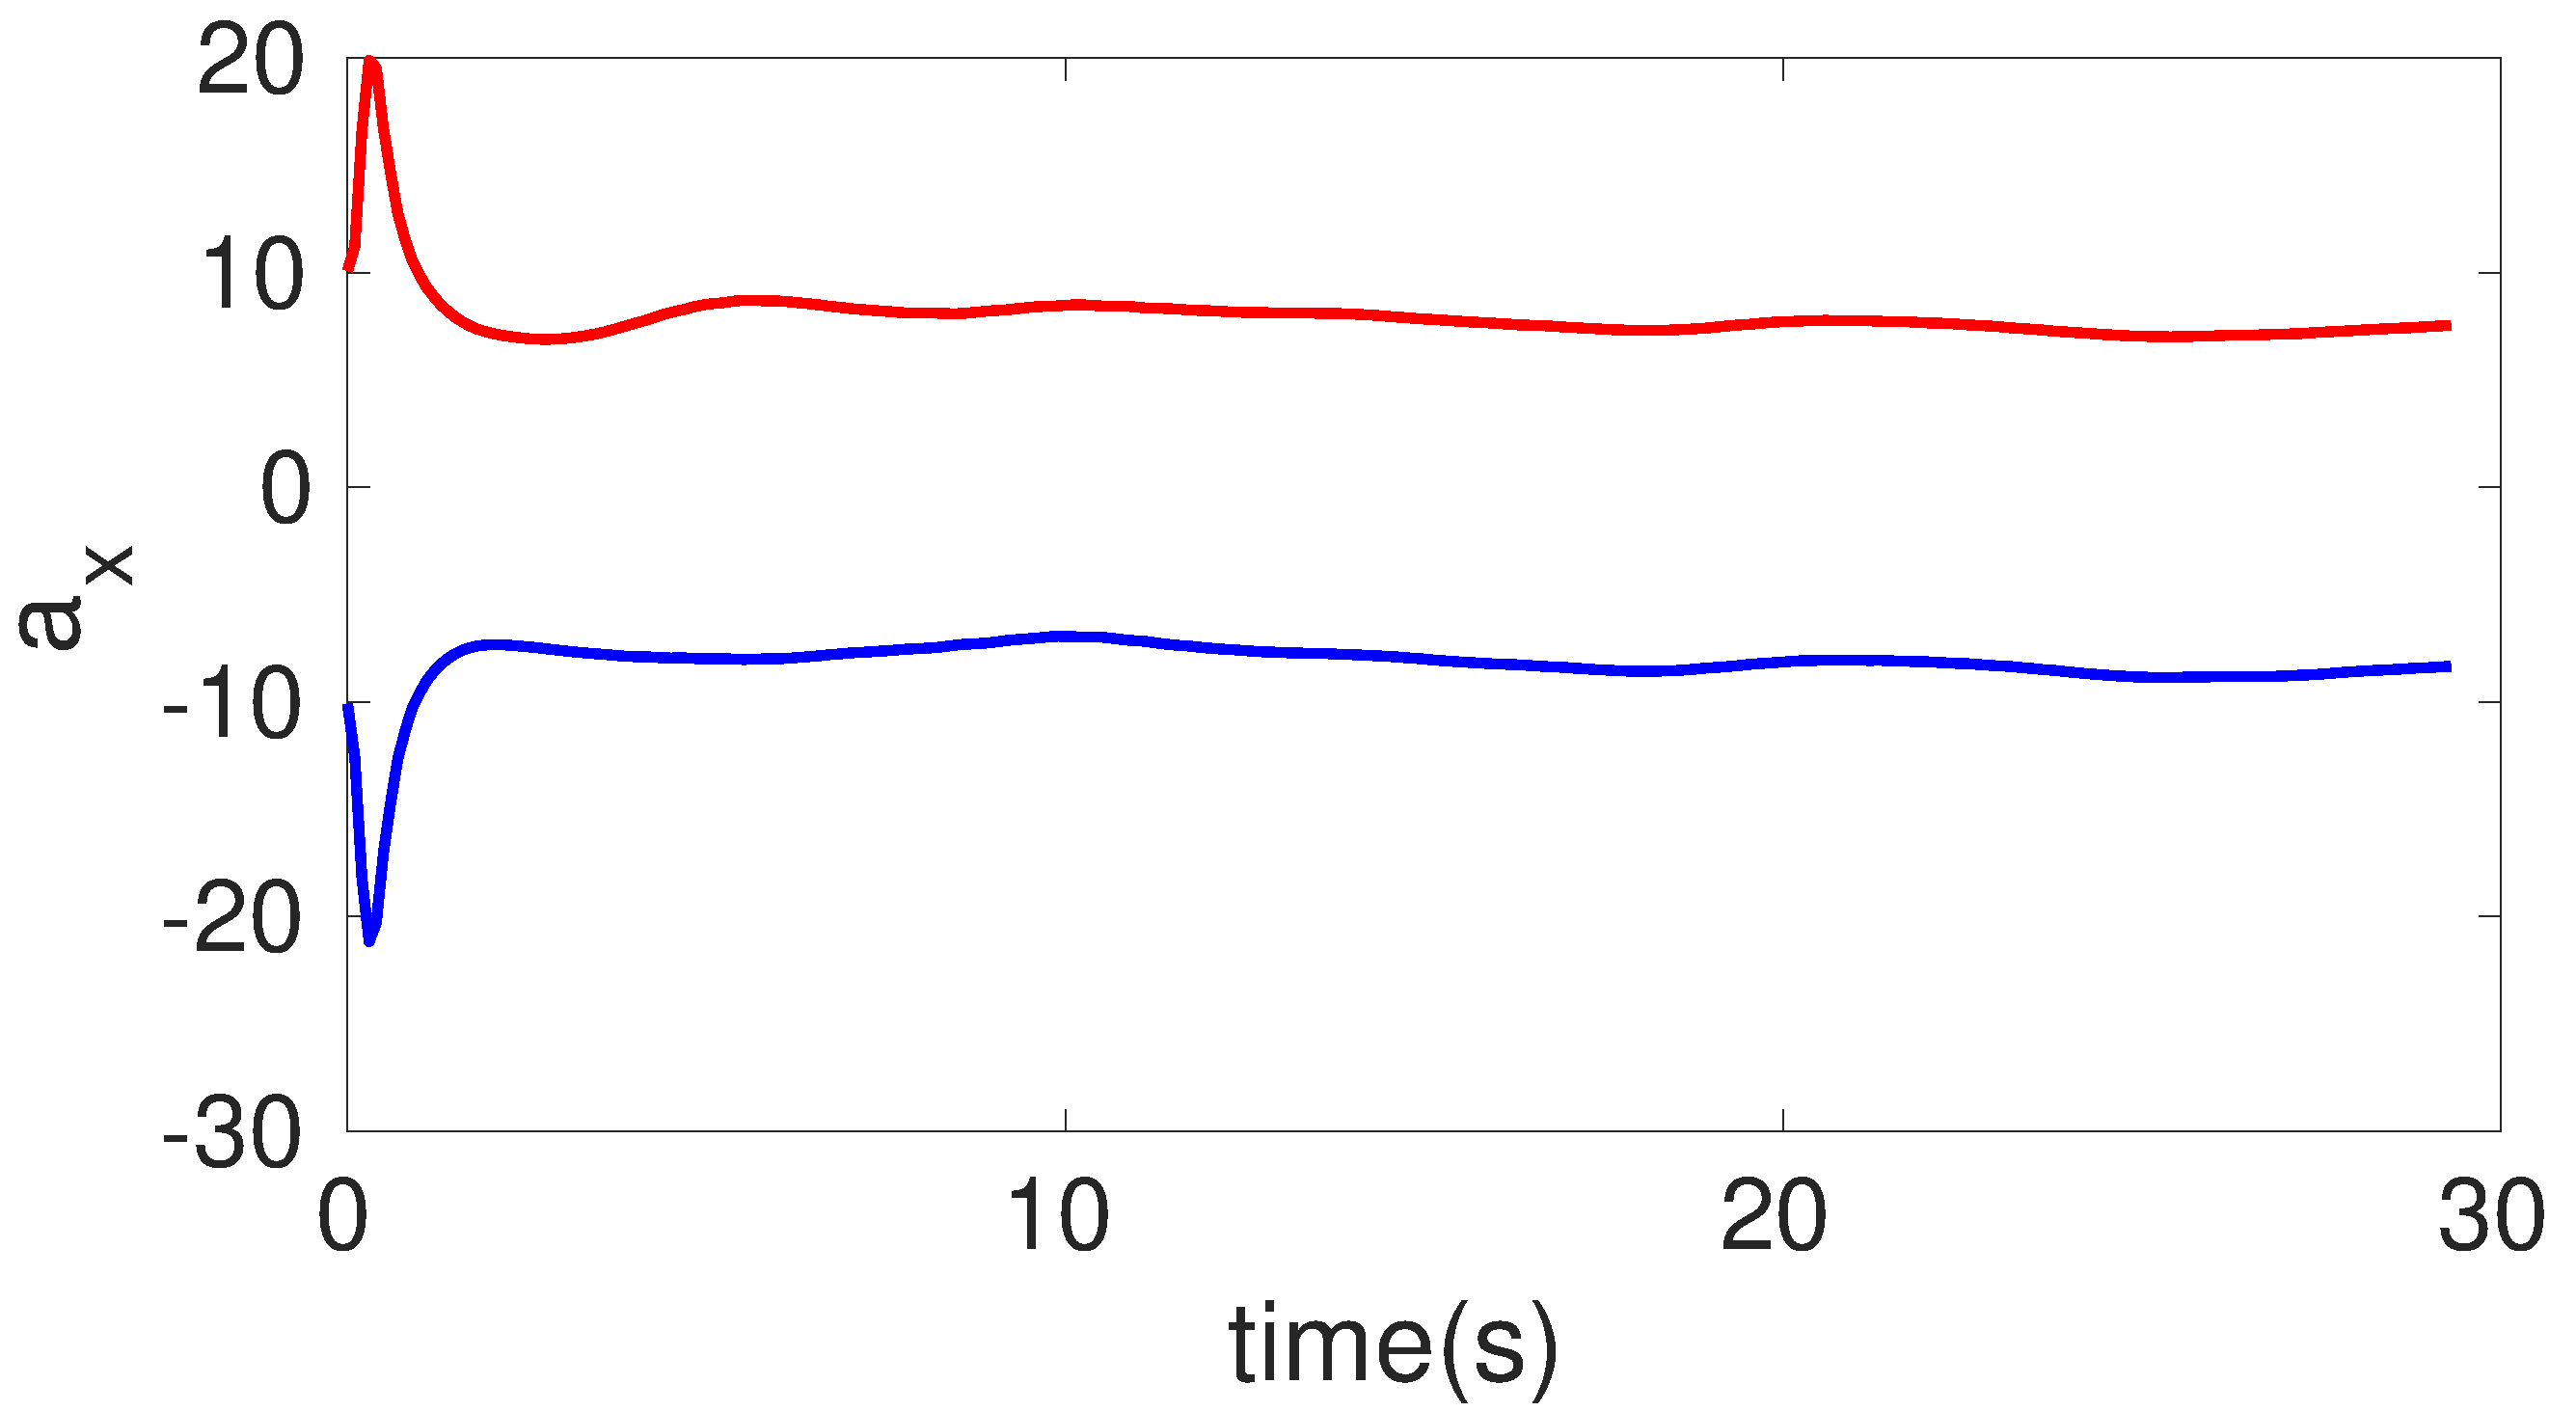
\includegraphics[width=\linewidth]{figures/Frad/s3caSMa_x}
\end{subfigure}
\begin{subfigure}{.5\linewidth}
\centering
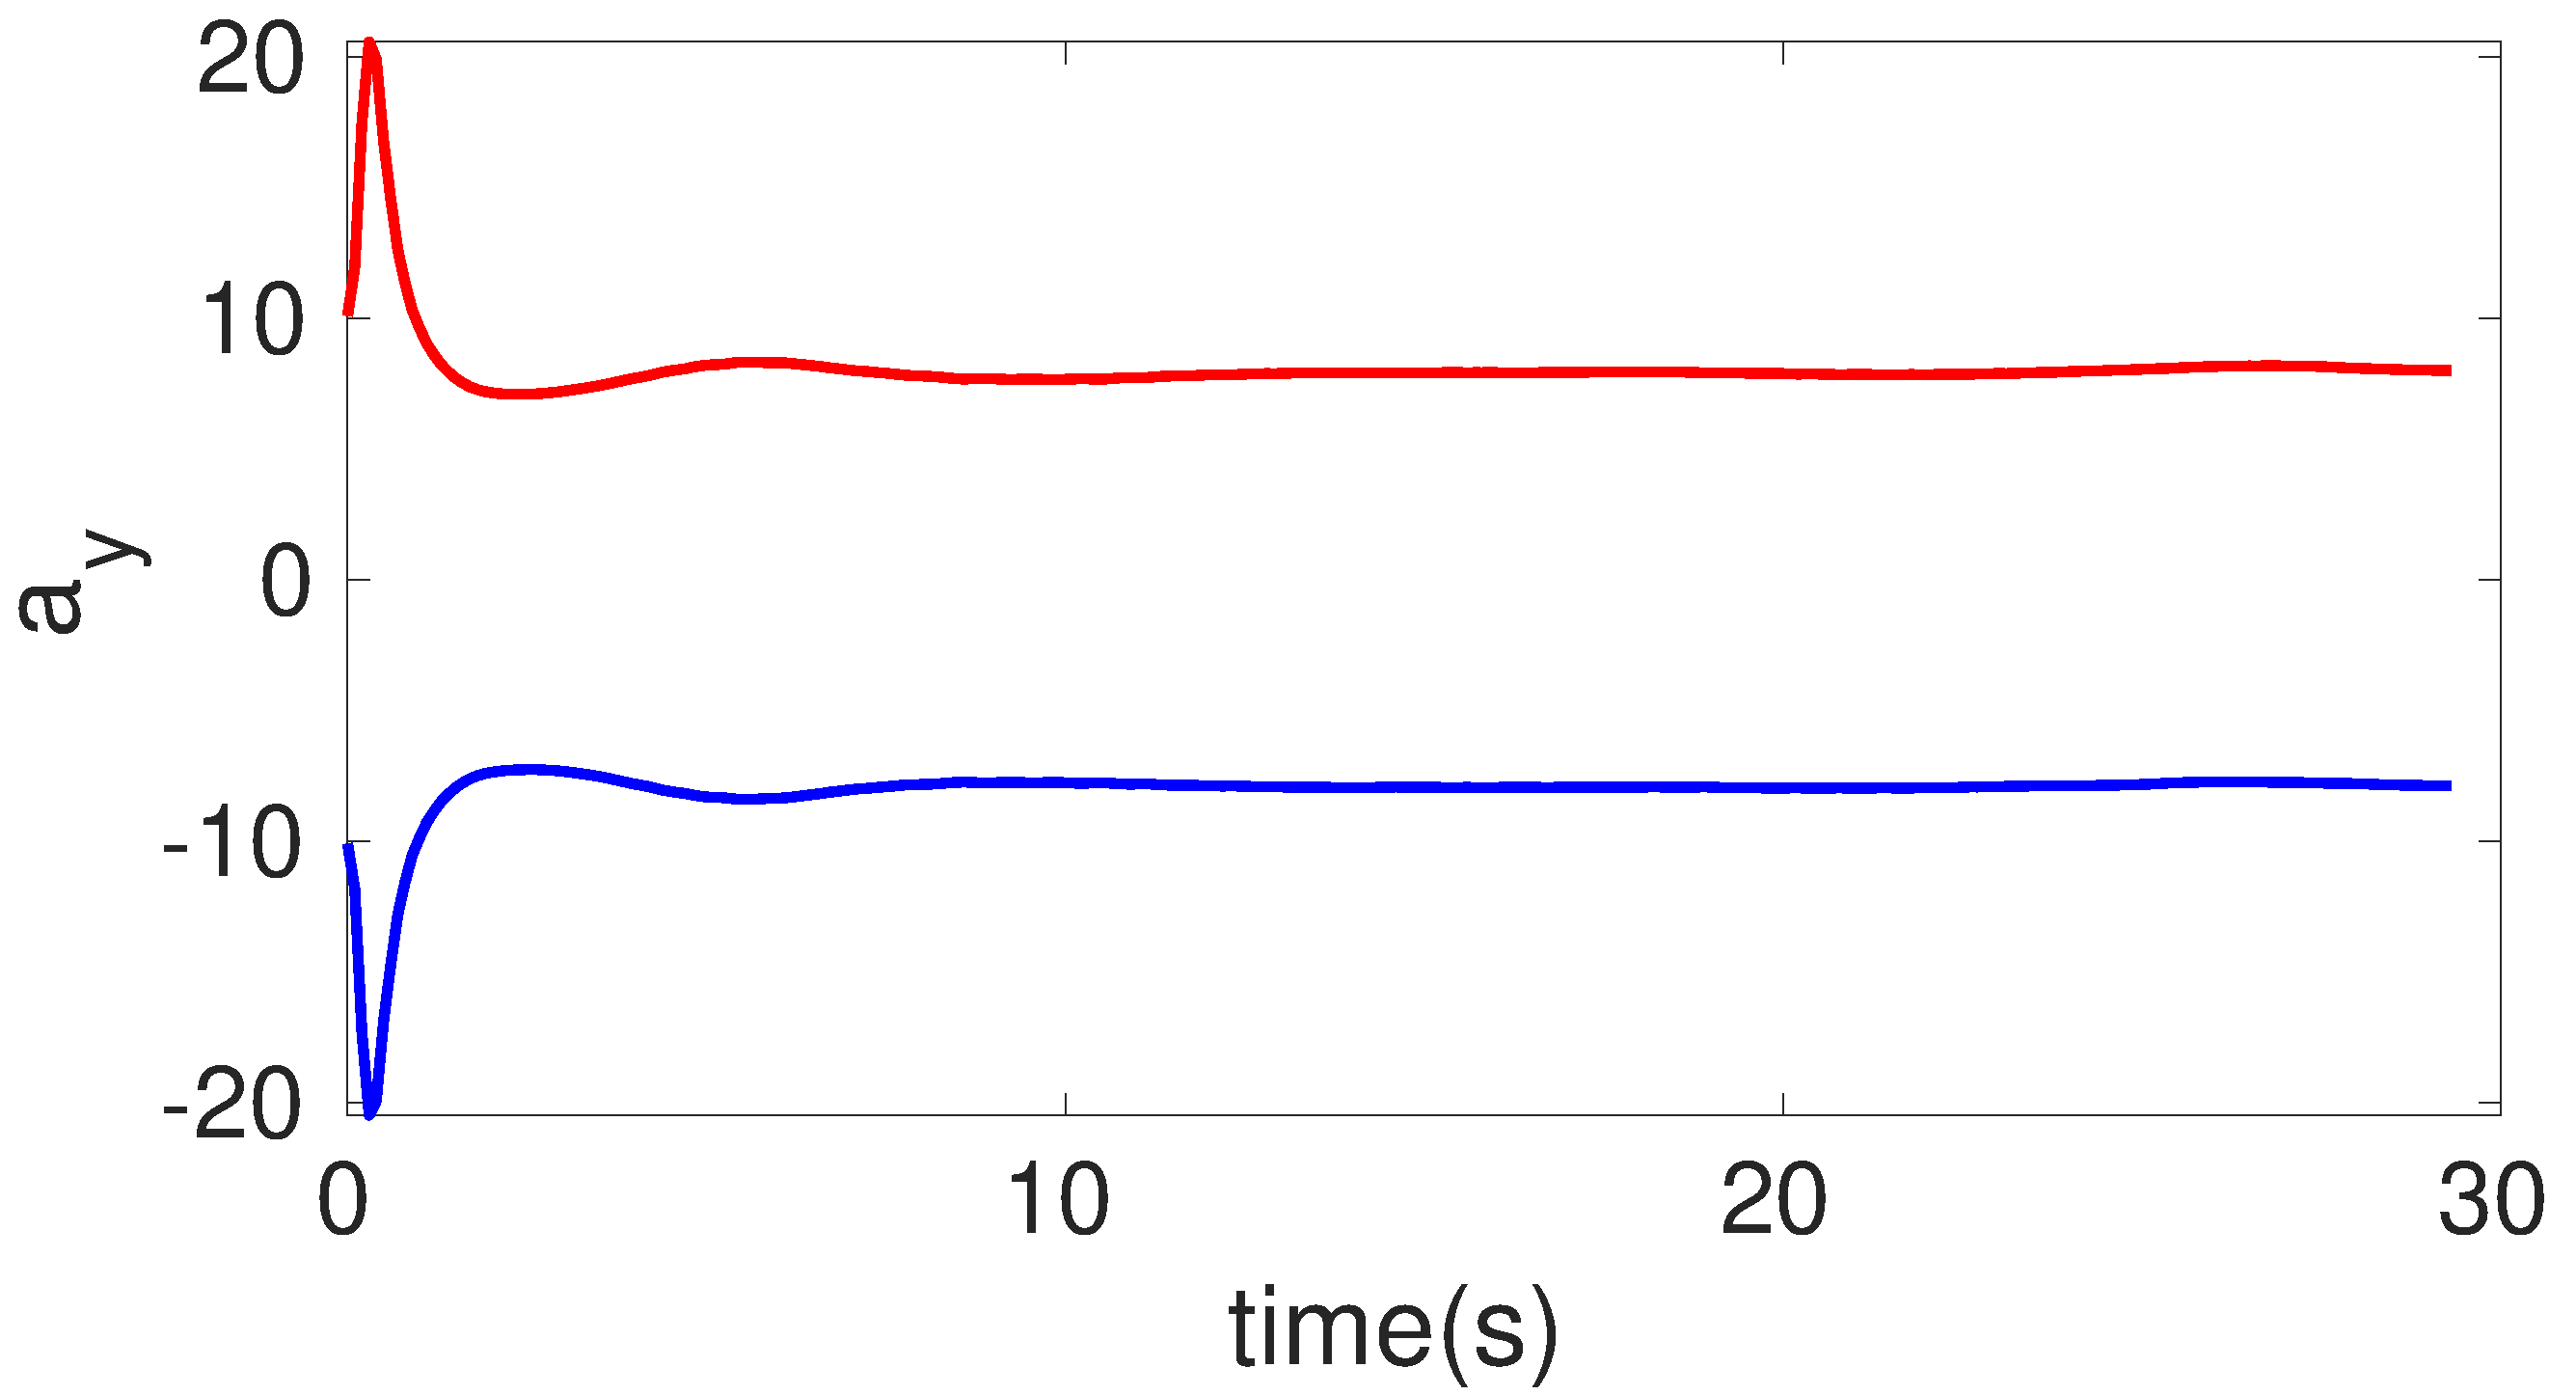
\includegraphics[width=\linewidth]{figures/Frad/s3caSMa_y}
\end{subfigure}
\caption{Estimation using the F-radius minimizer and the constant acceleration model}
\end{figure}

\begin{figure}[h]
\hspace*{\fill} 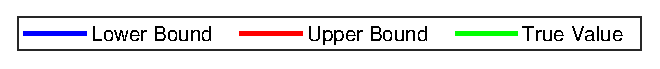
\includegraphics[scale=0.8]{figures/legend}\\\\
\begin{subfigure}{.5\linewidth}
\centering
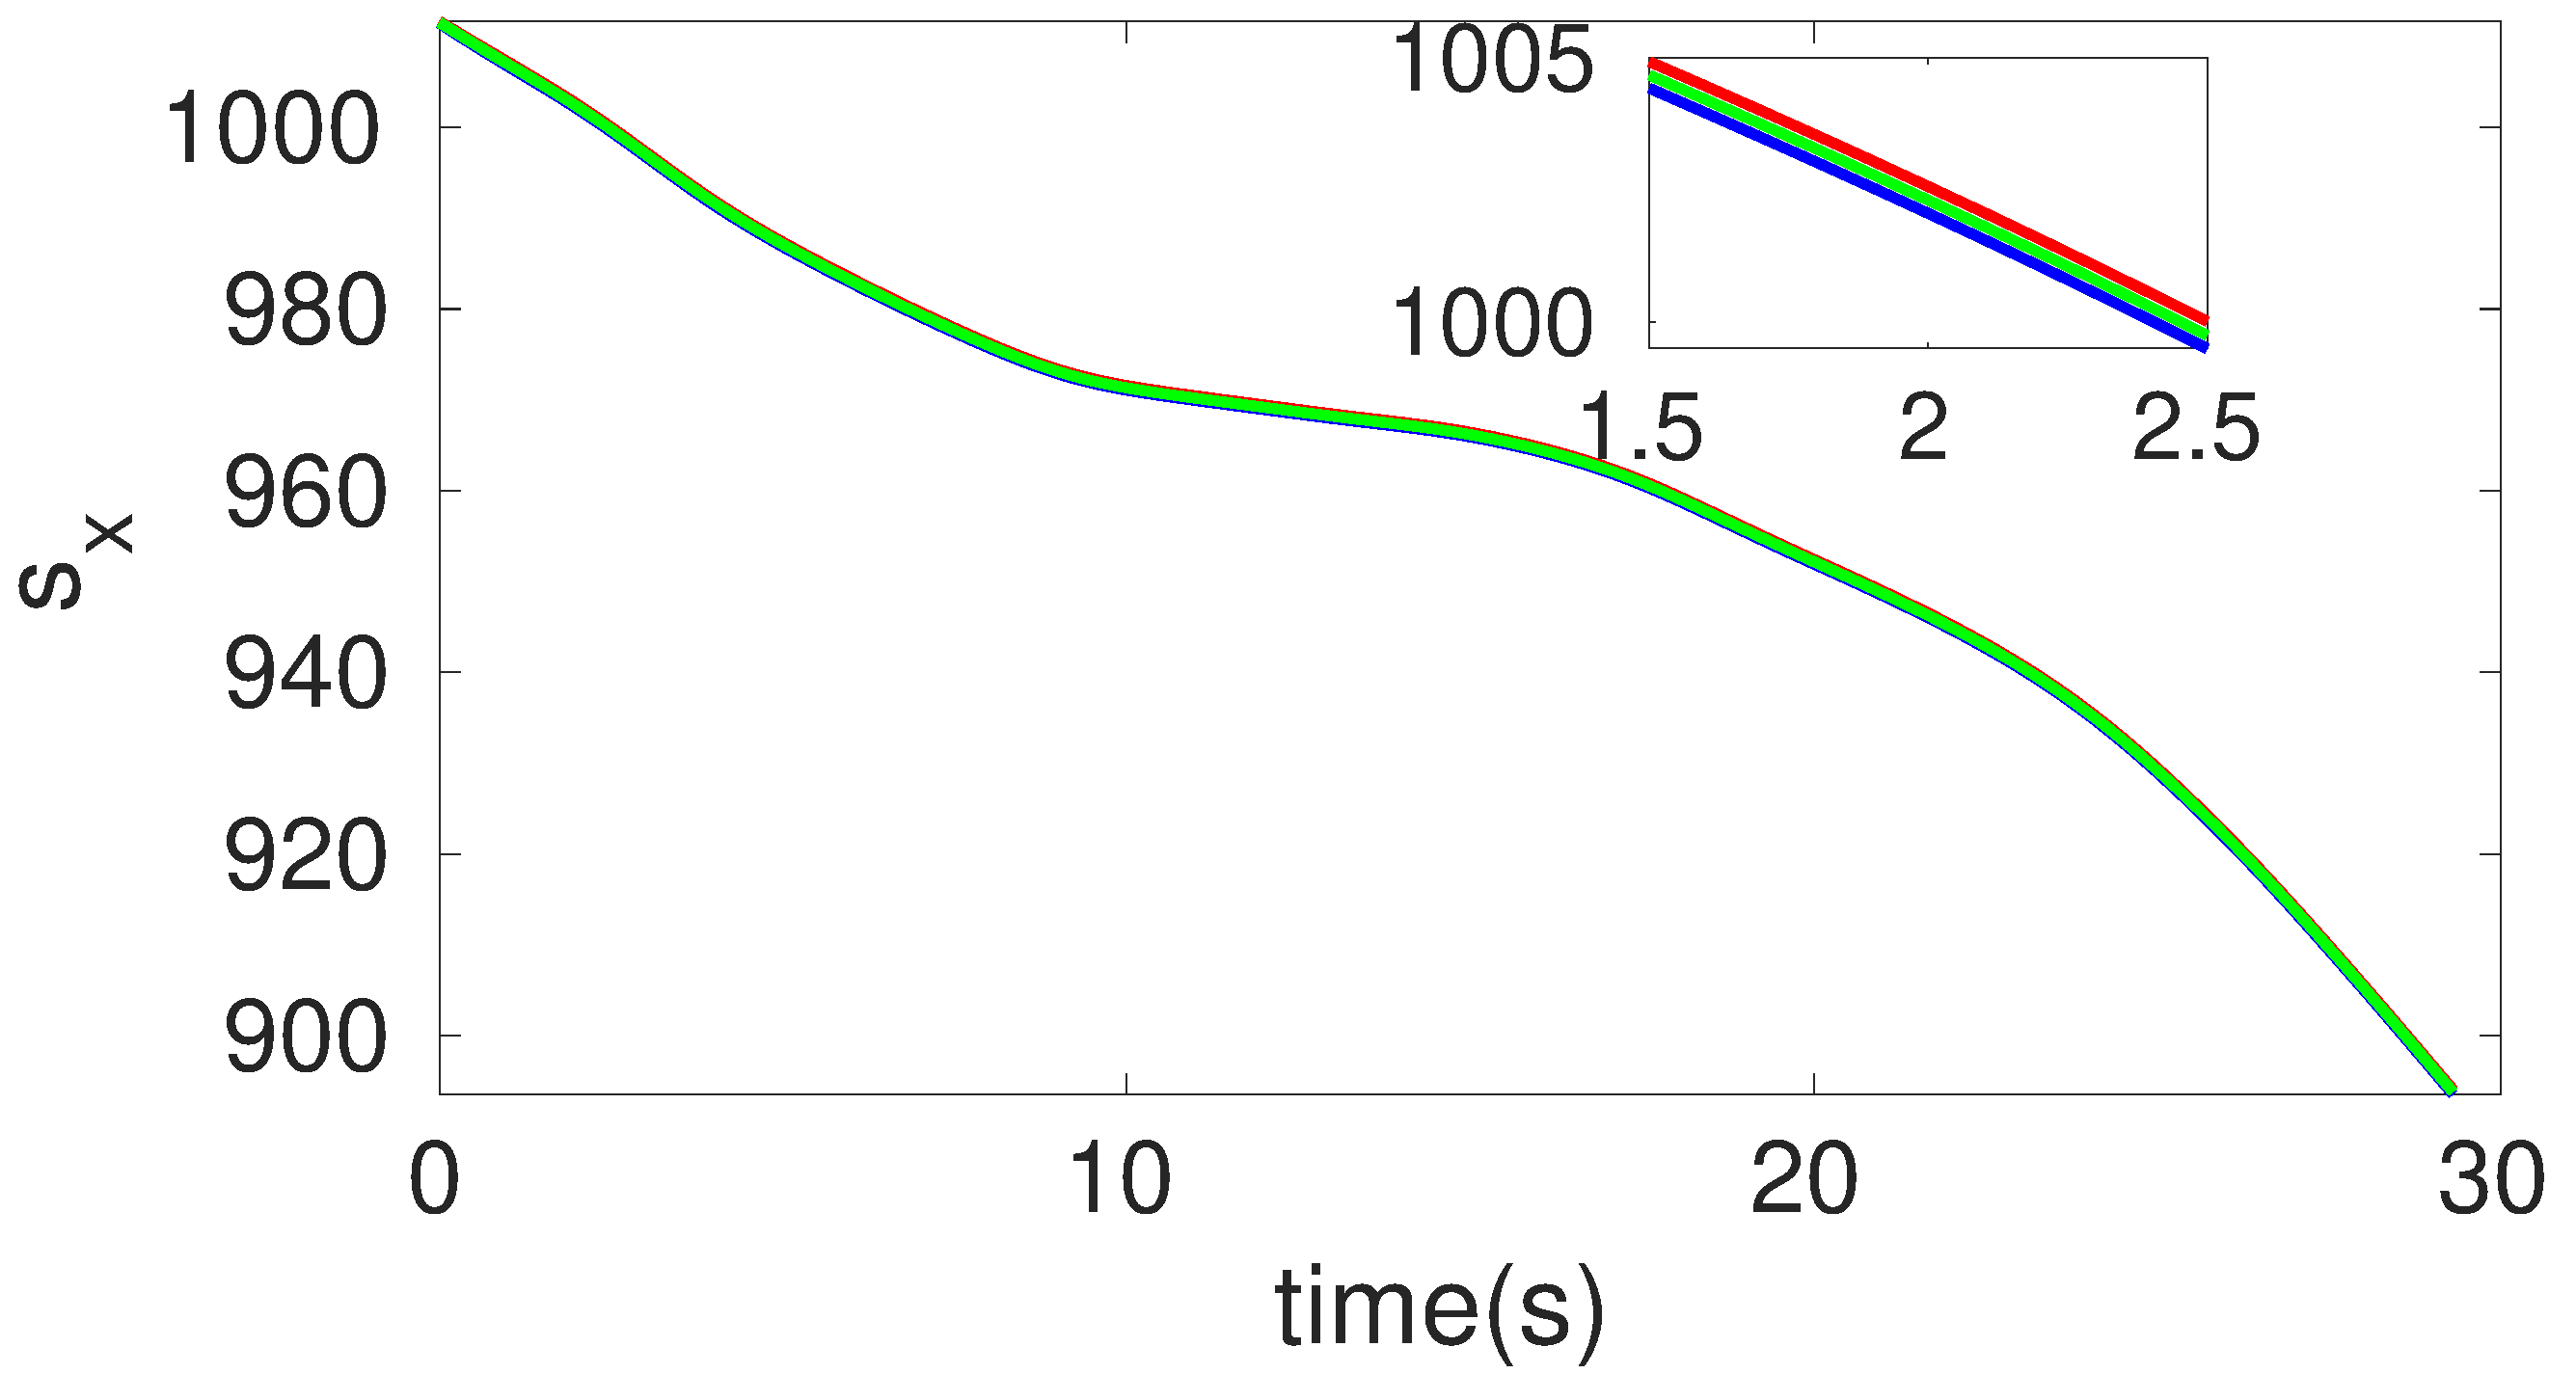
\includegraphics[width=\linewidth]{figures/Frad/s3pmSMs_x}
\end{subfigure}
\begin{subfigure}{.5\linewidth}
\centering
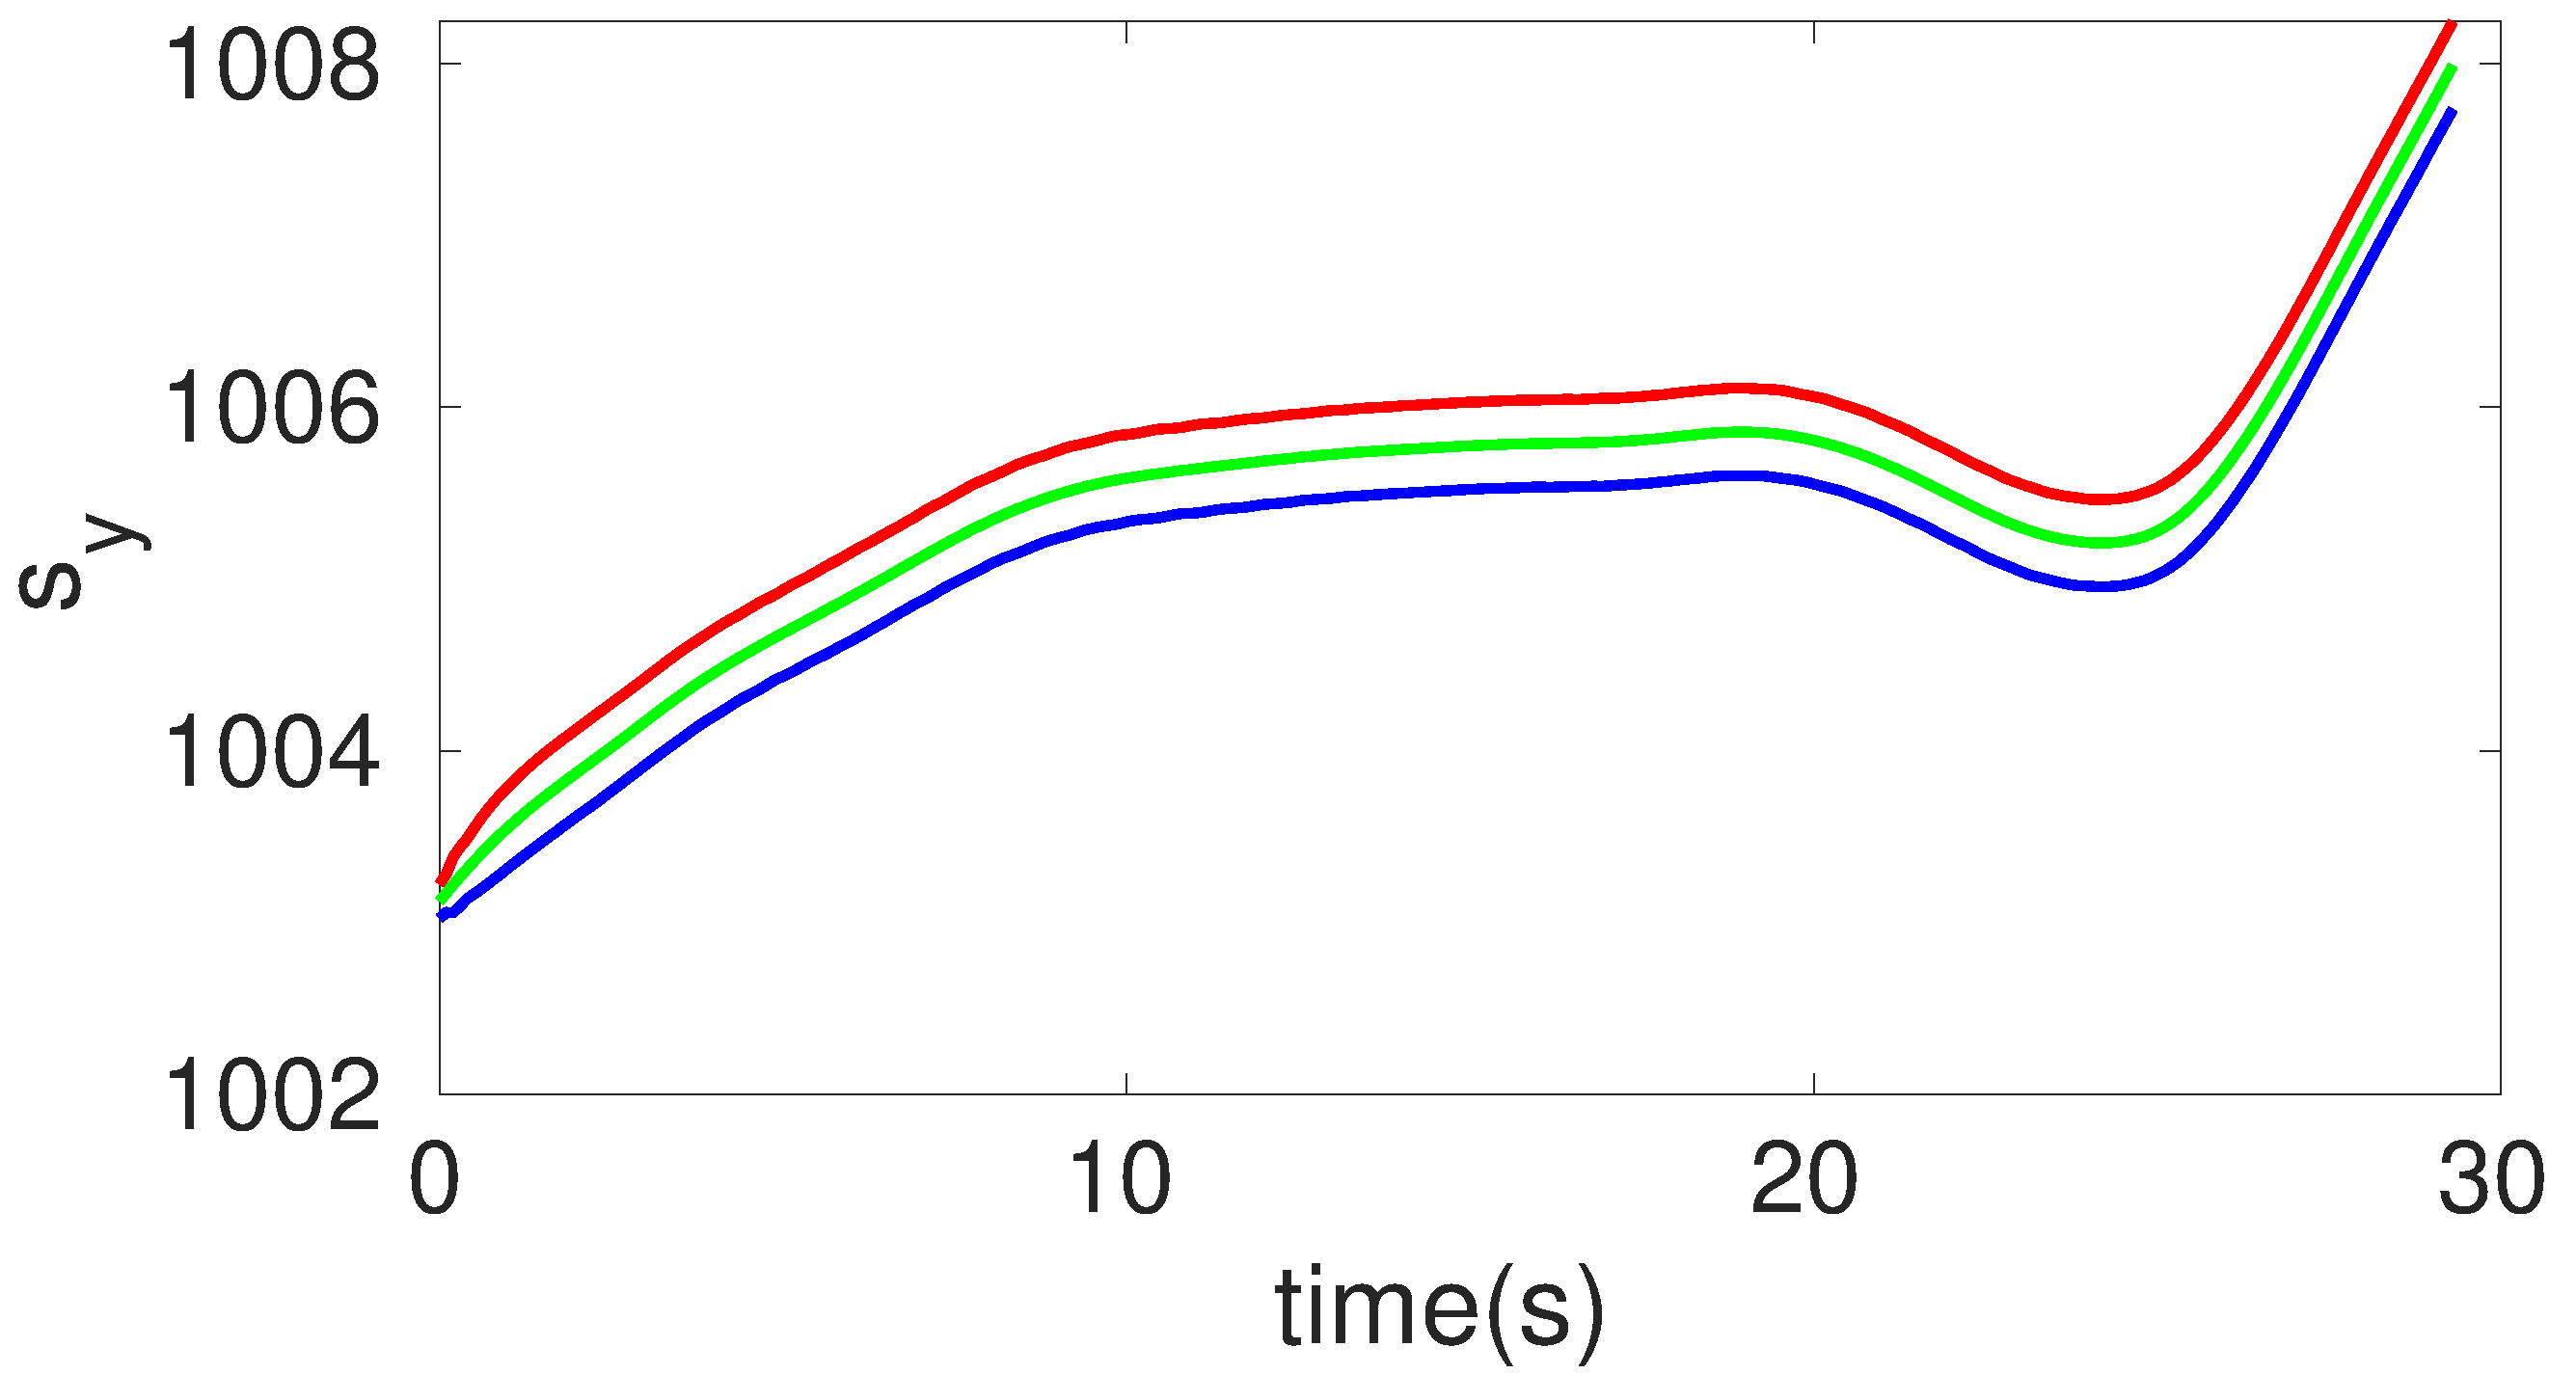
\includegraphics[width=\linewidth]{figures/Frad/s3pmSMs_y}
\end{subfigure}
\begin{subfigure}{.5\linewidth}
\centering
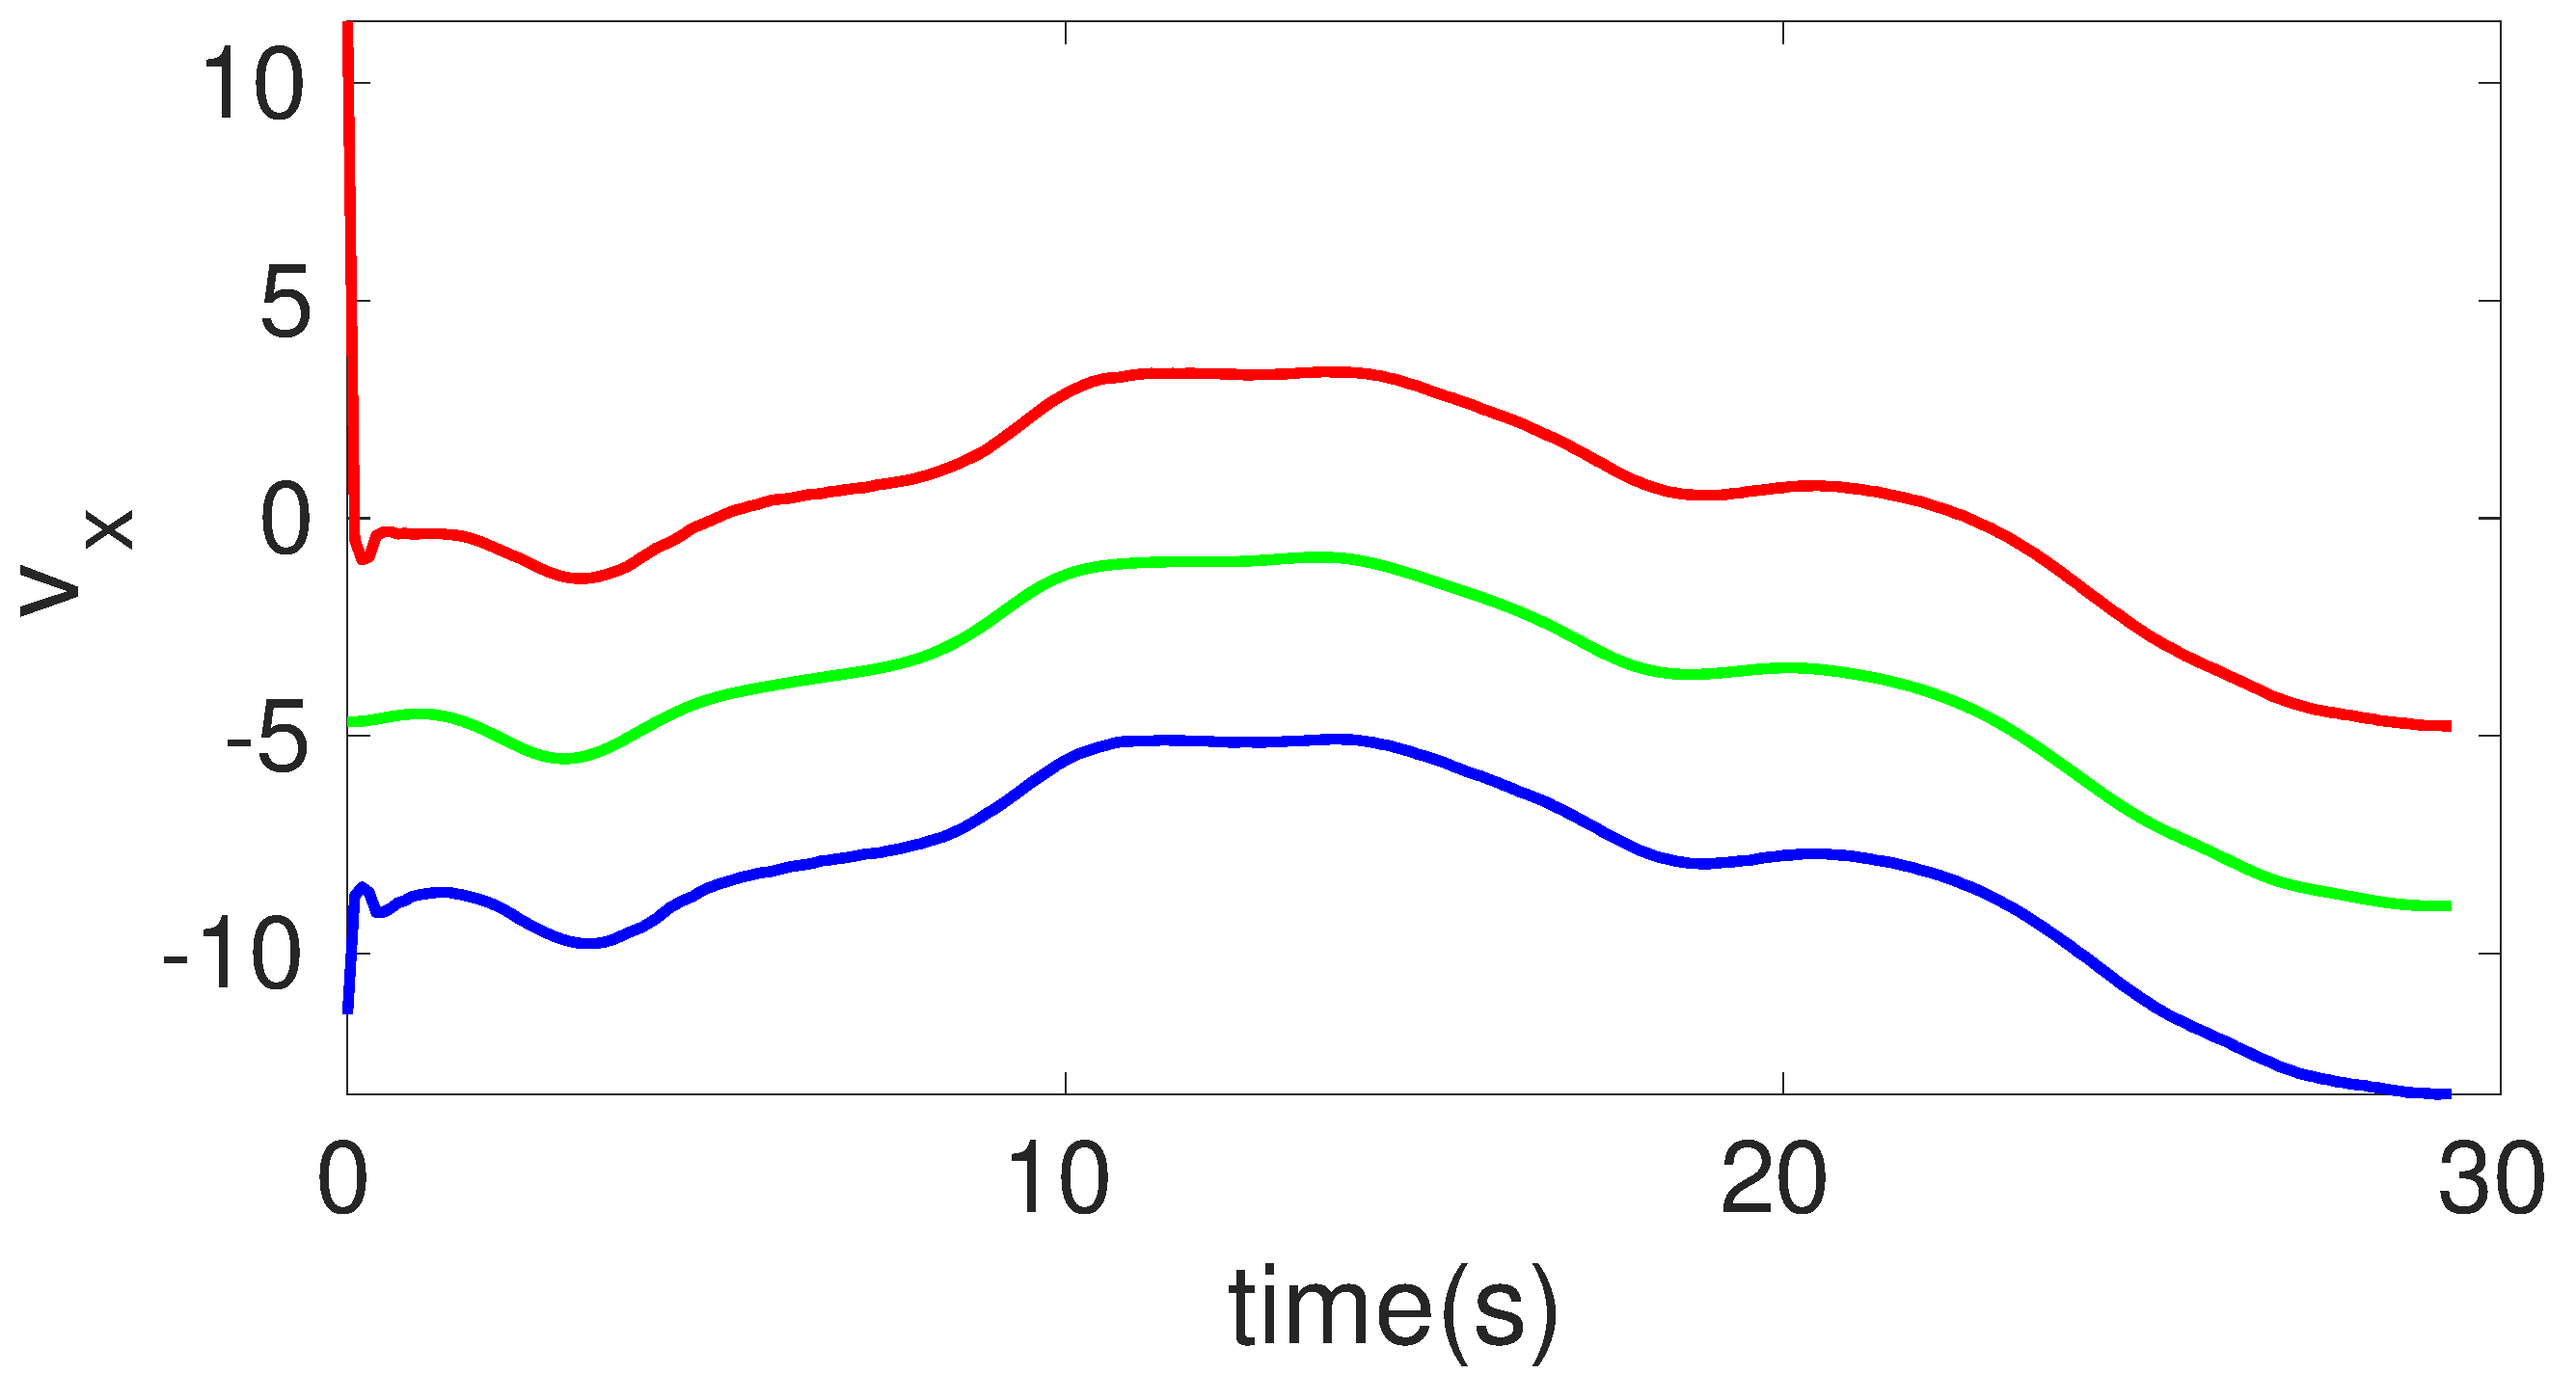
\includegraphics[width=\linewidth]{figures/Frad/s3pmSMv_x}
\end{subfigure}
\begin{subfigure}{.5\linewidth}
\centering
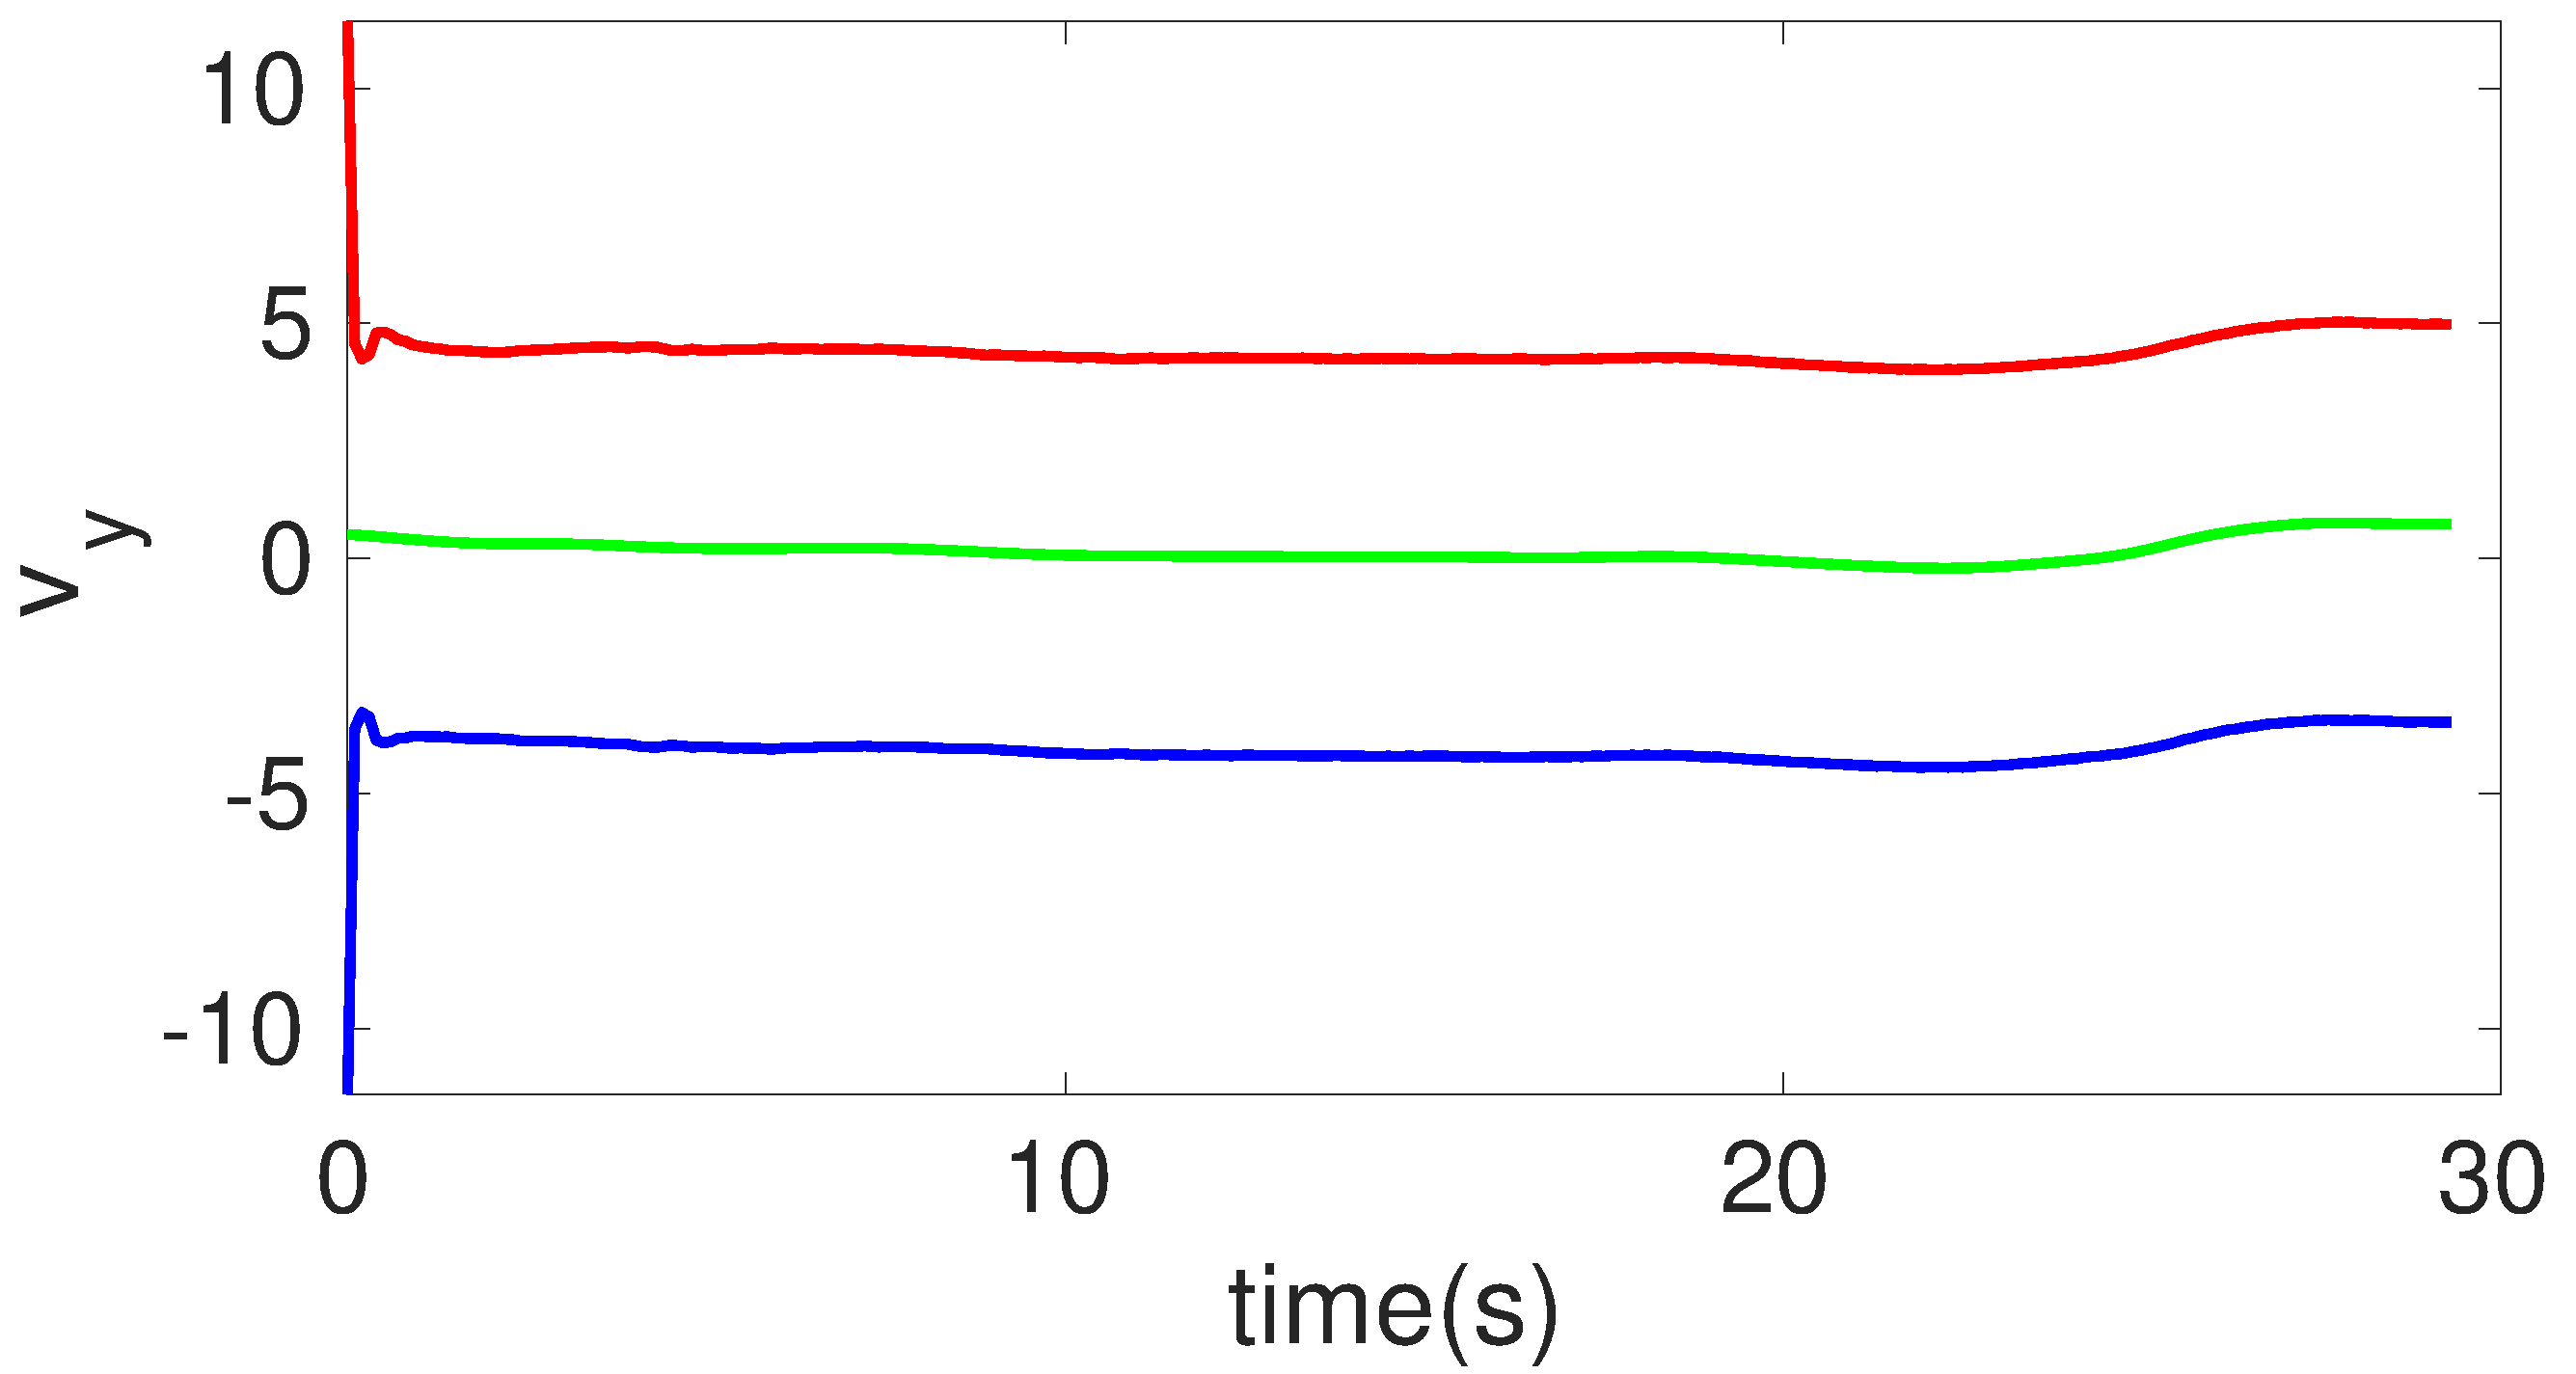
\includegraphics[width=\linewidth]{figures/Frad/s3pmSMv_y}
\end{subfigure}
\begin{subfigure}{.5\linewidth}
\centering
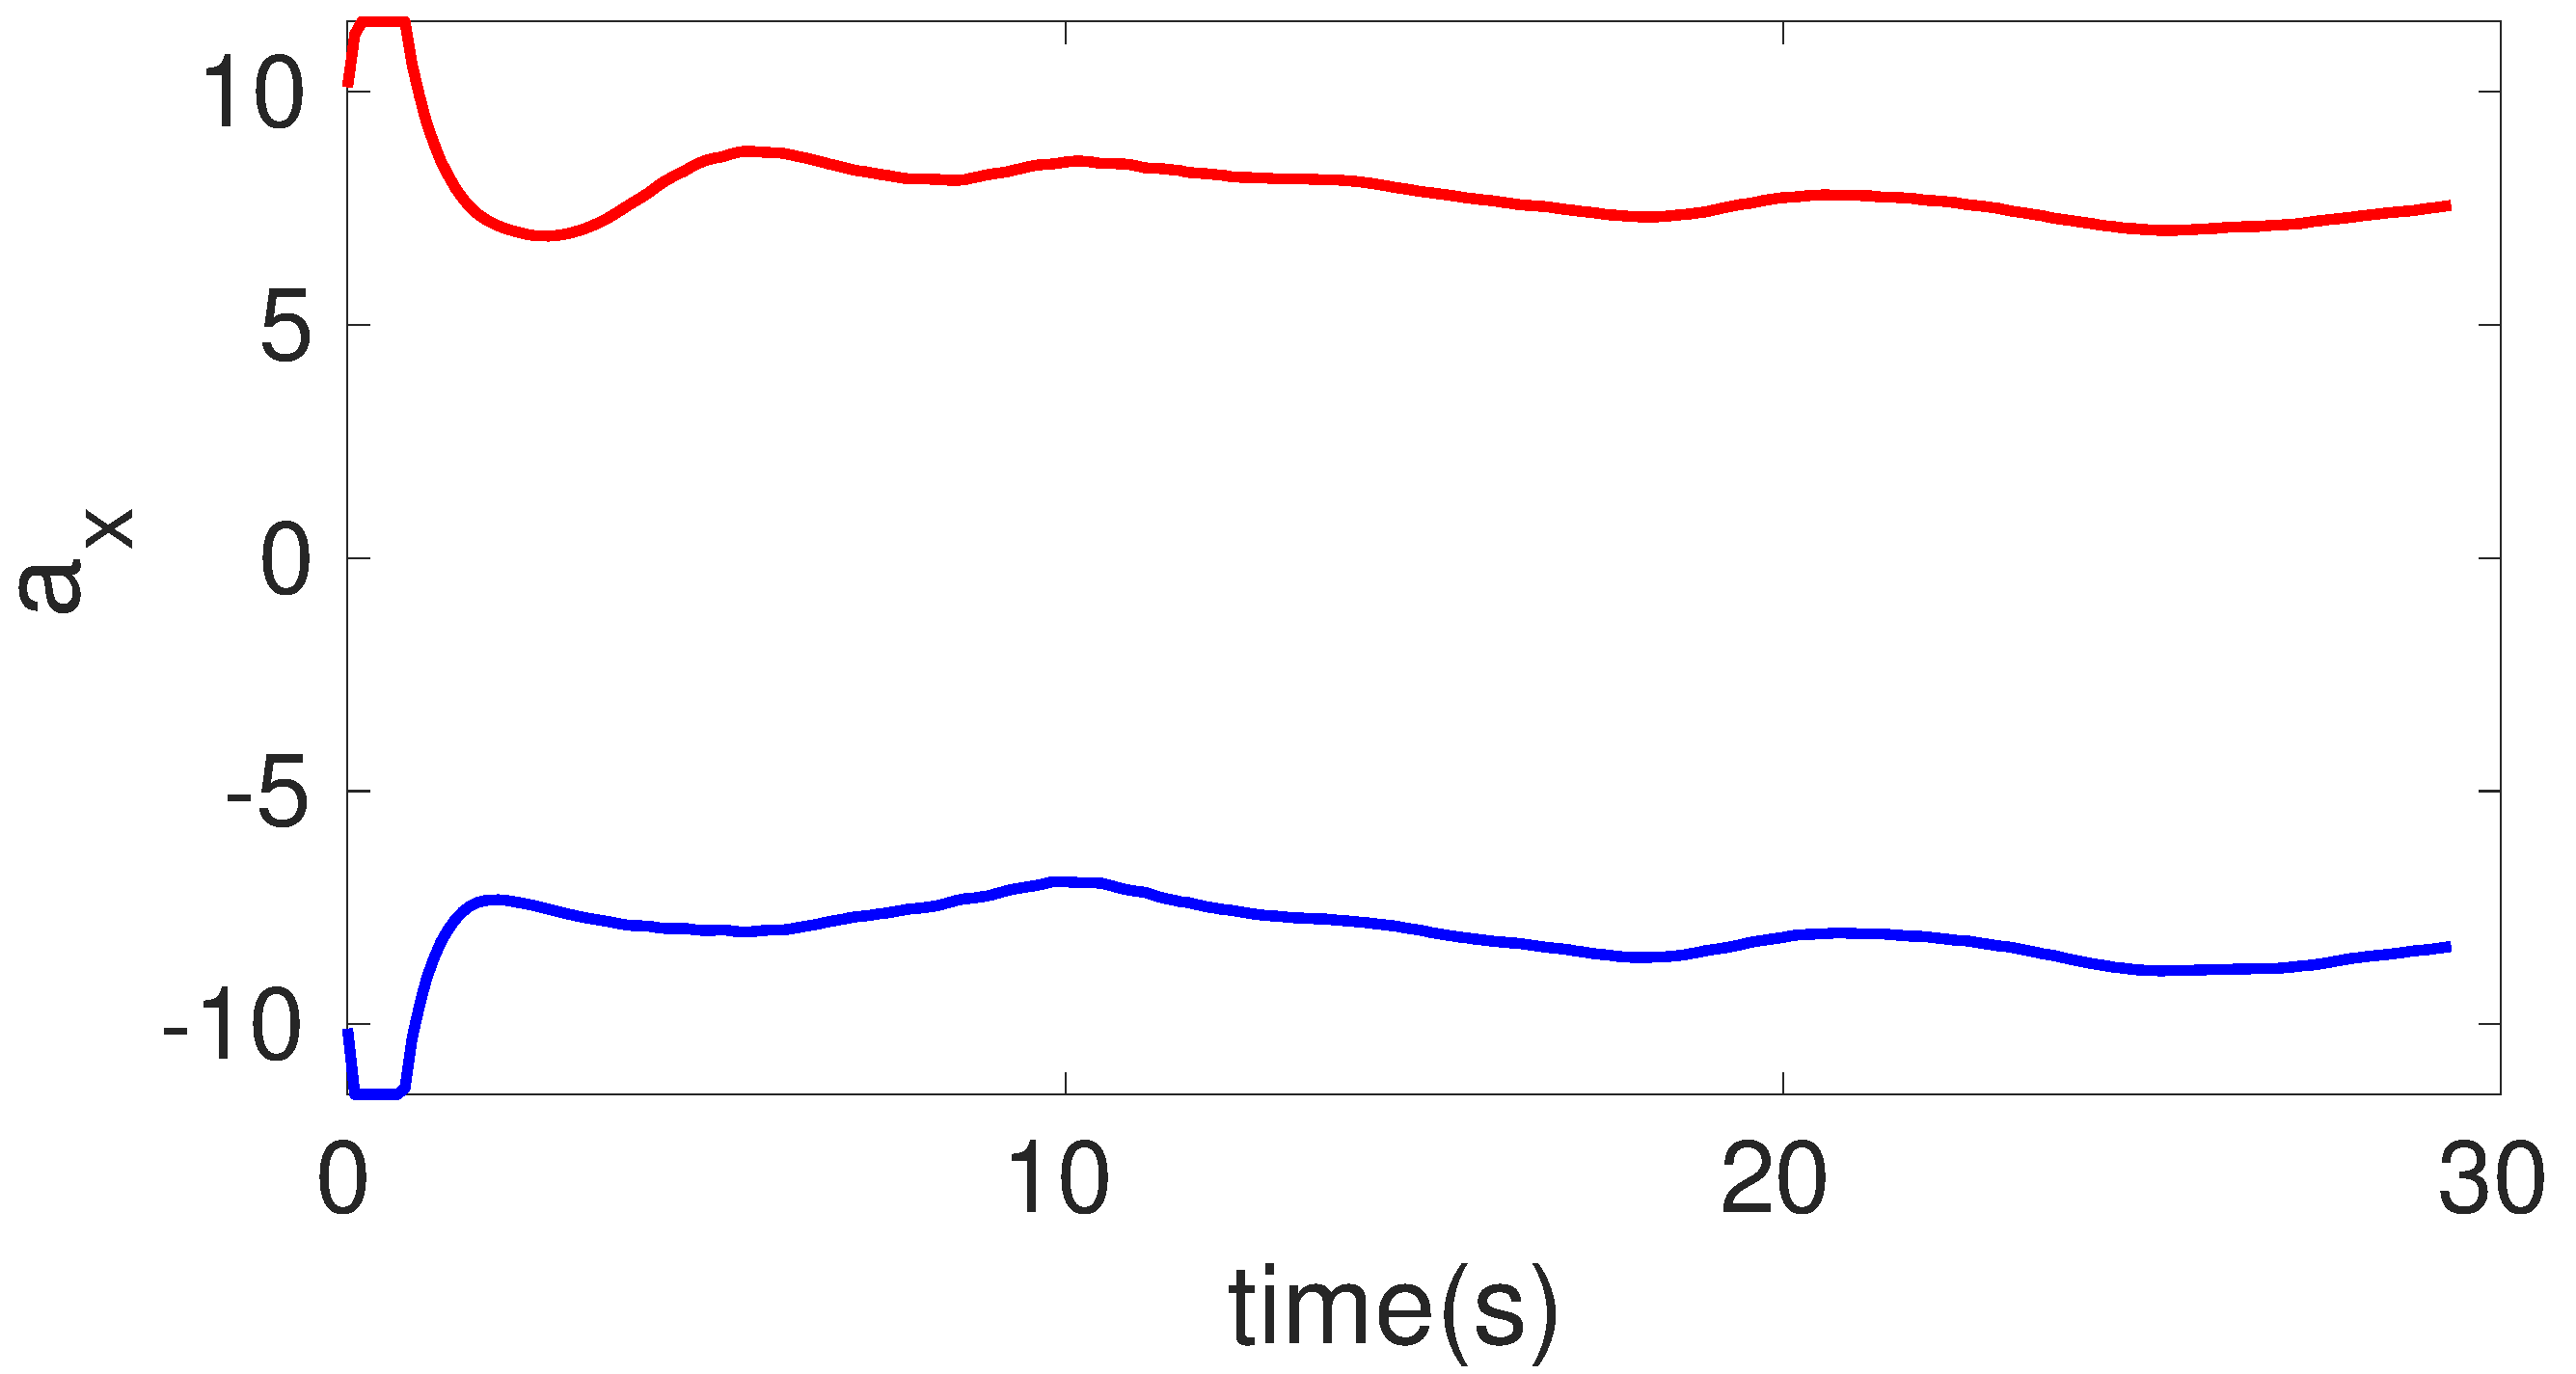
\includegraphics[width=\linewidth]{figures/Frad/s3pmSMa_x}
\end{subfigure}
\begin{subfigure}{.5\linewidth}
\centering
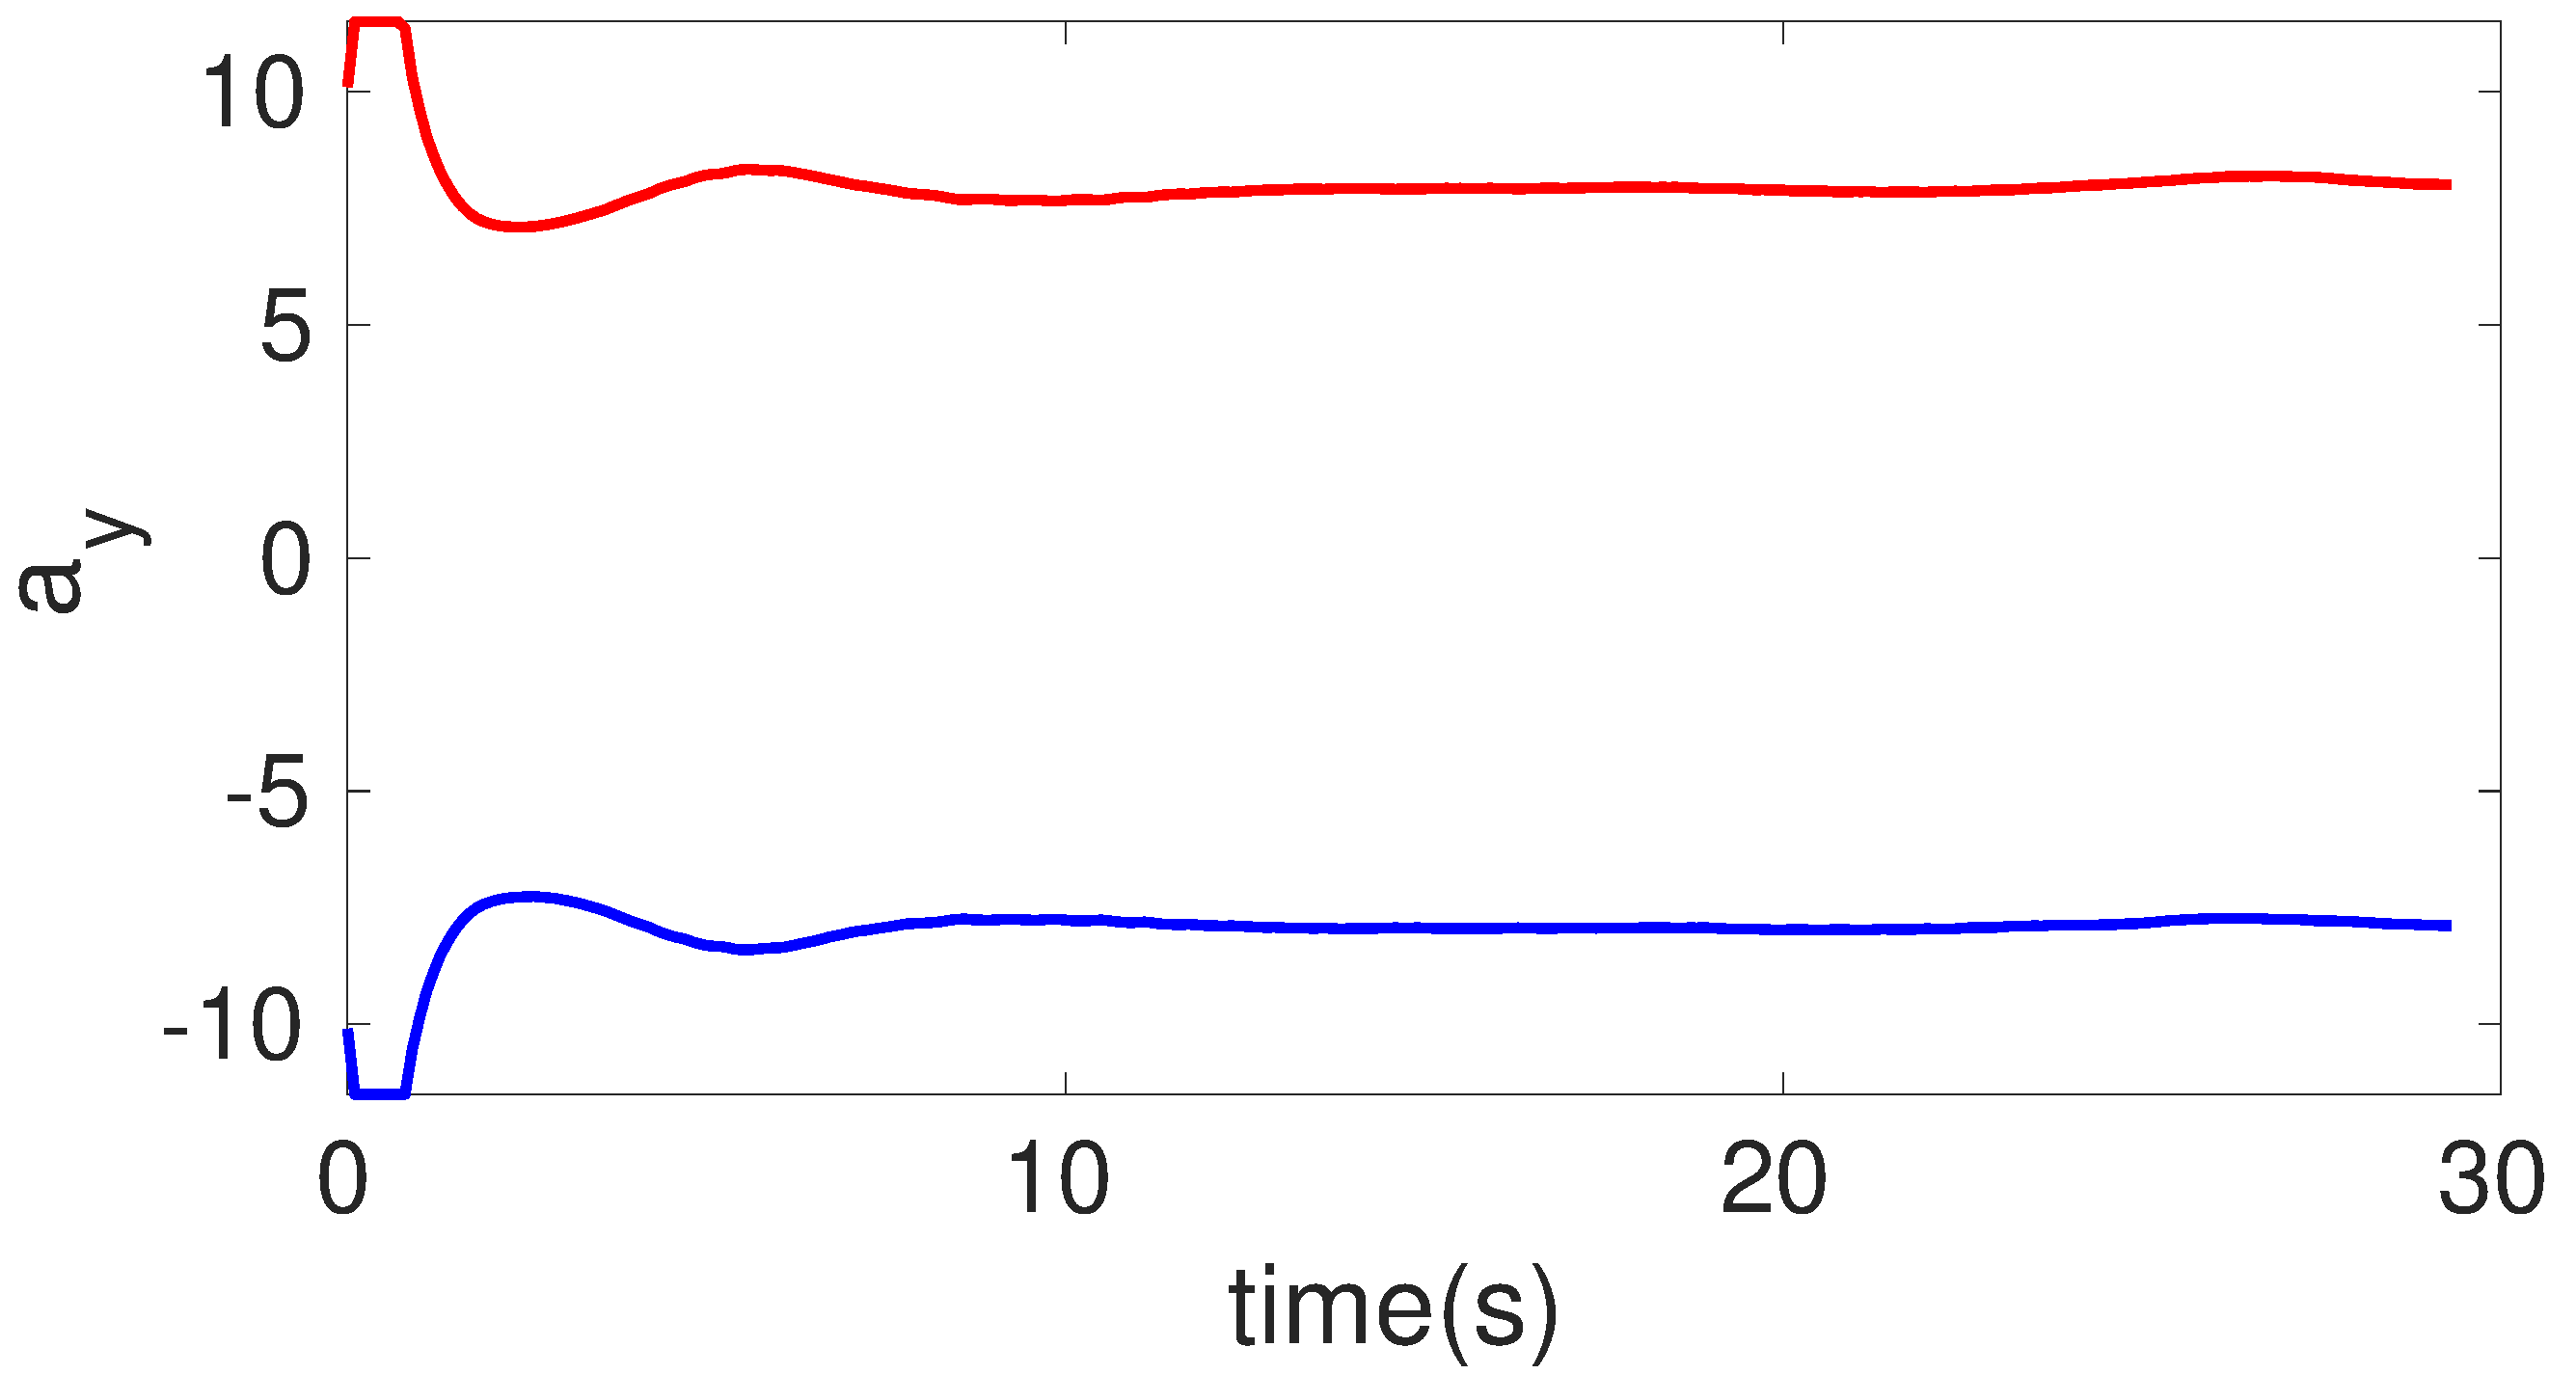
\includegraphics[width=\linewidth]{figures/Frad/s3pmSMa_y}
\end{subfigure}
\caption{Estimation using the F-radius minimizer and the point-mass model}
\end{figure}

\clearpage
\subsection{Segment Minimization using P-Radius}
\FloatBarrier
\begin{figure}[h]
\hspace*{\fill} 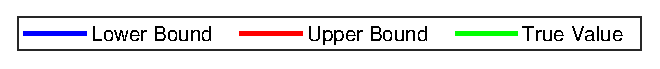
\includegraphics[scale=0.8]{figures/legend}\\\\
\begin{subfigure}{.5\linewidth}
\centering
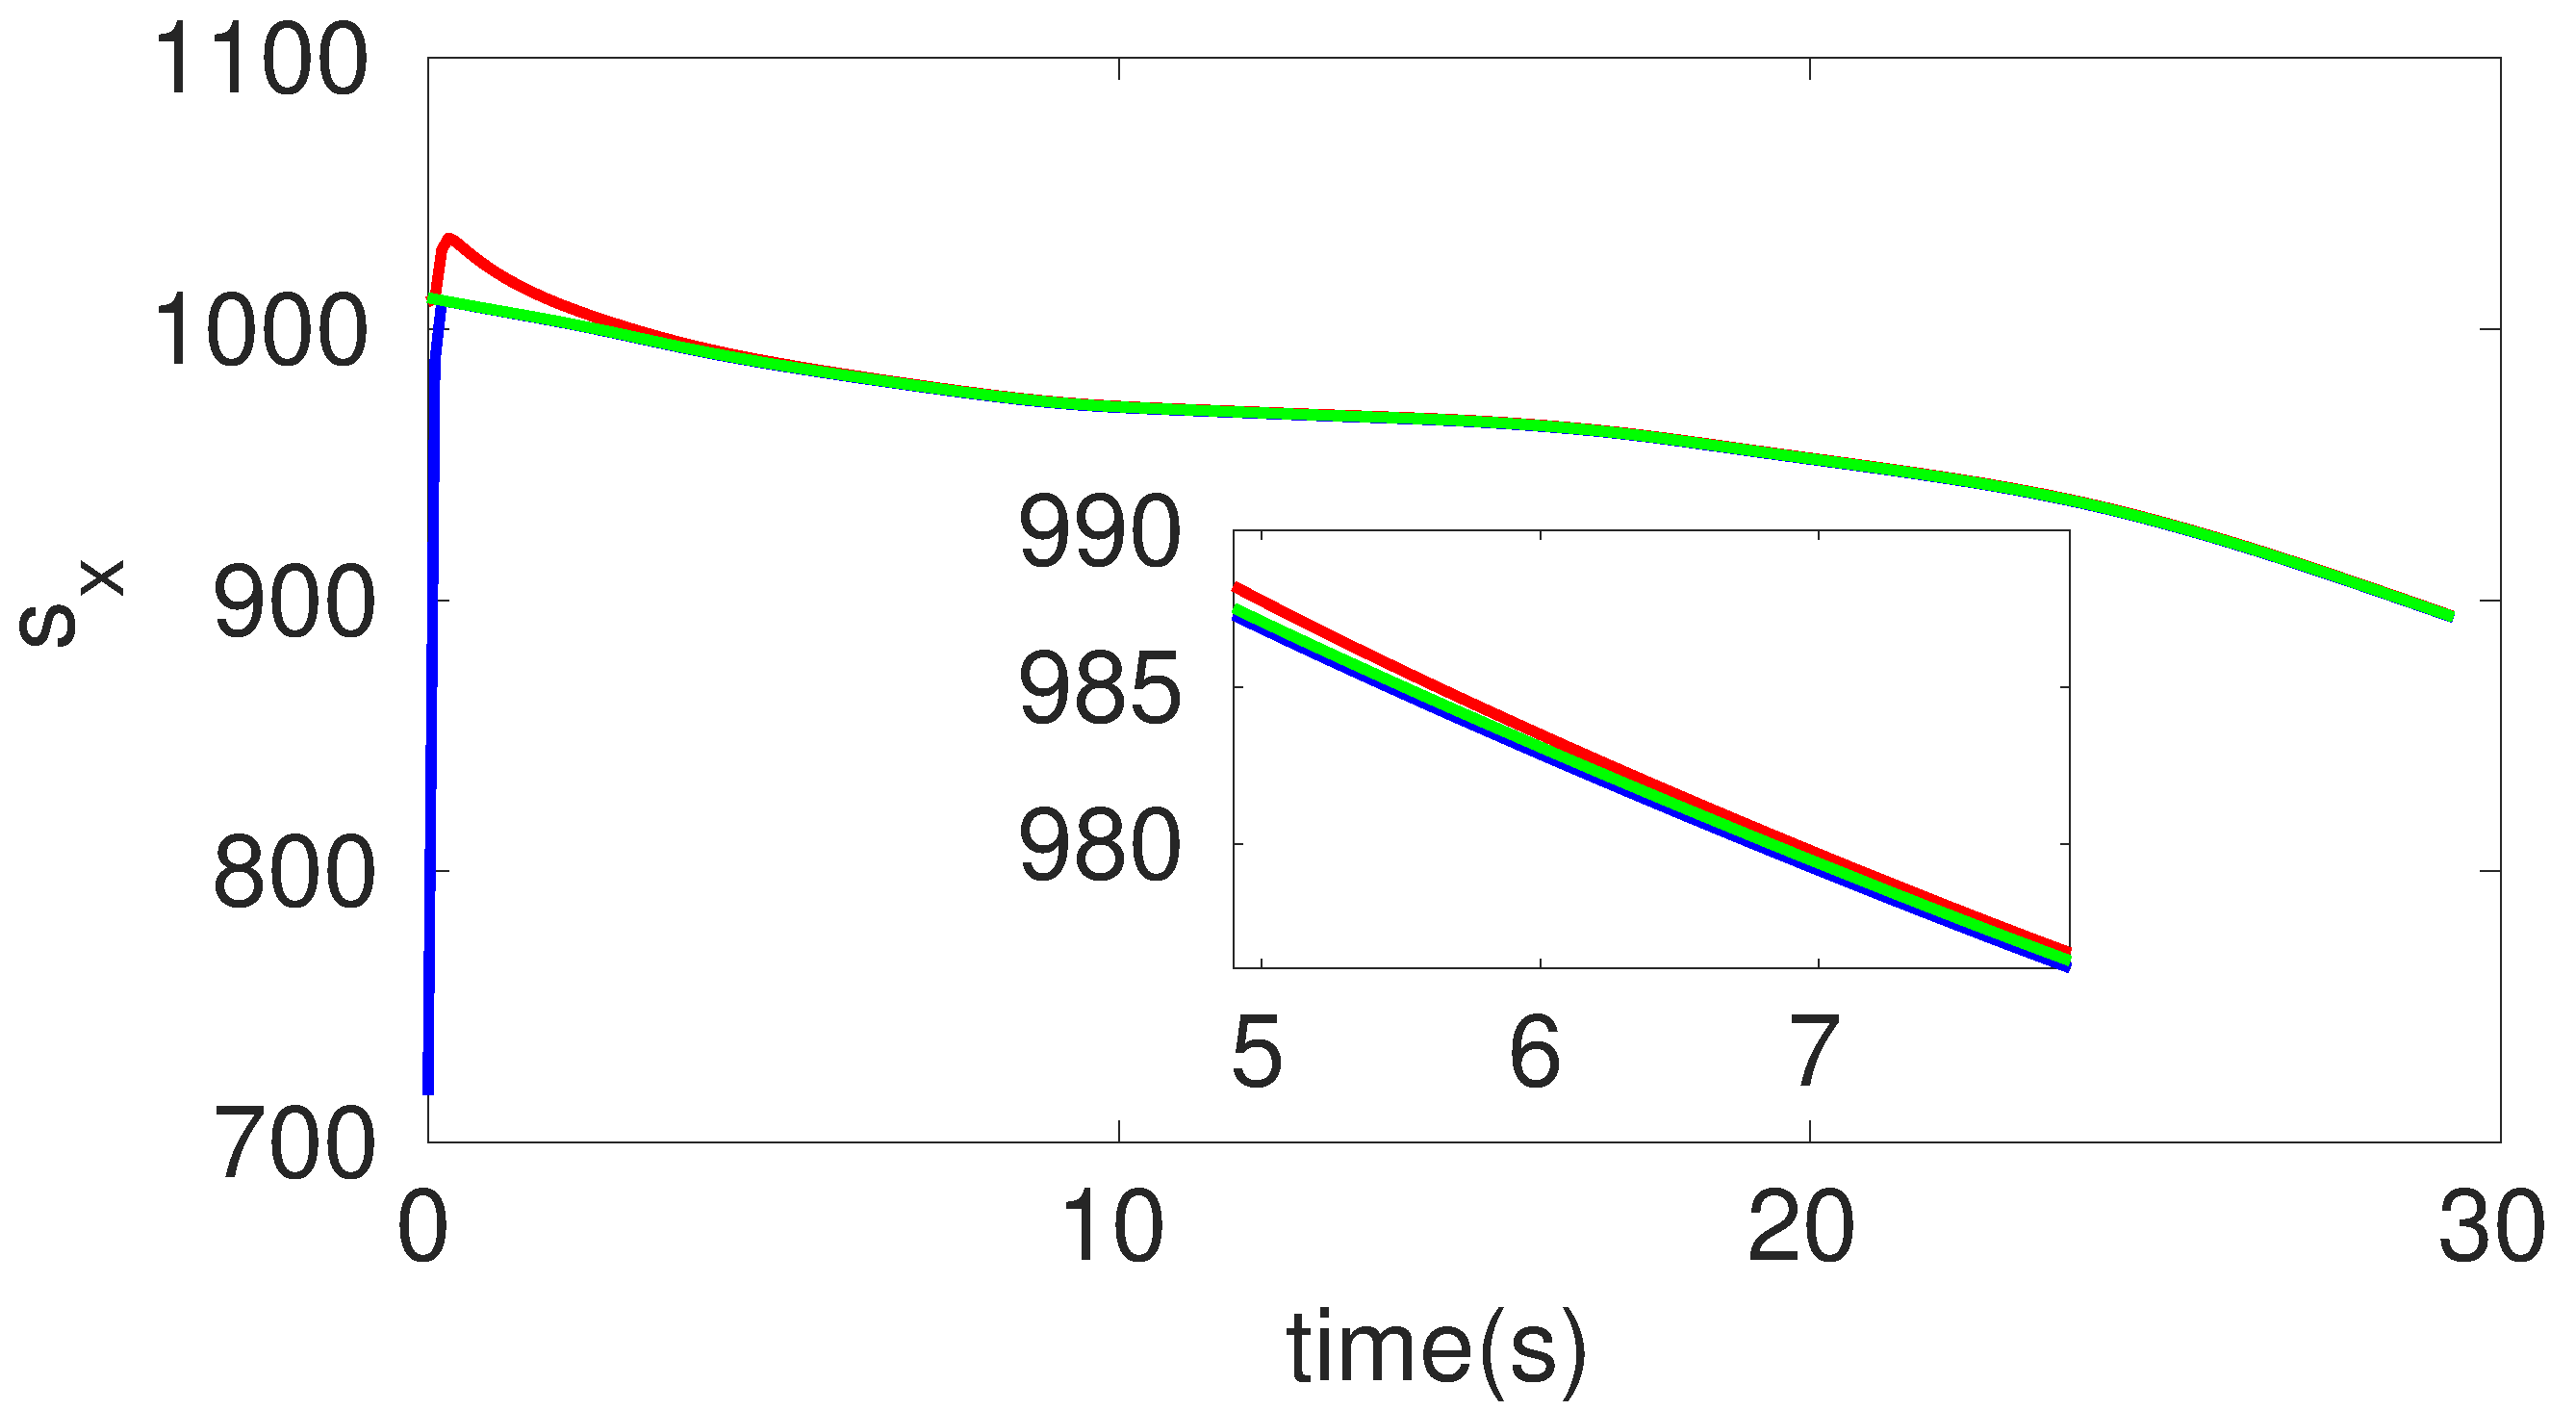
\includegraphics[width=\linewidth]{figures/Prad/s3cvprads_x}
\end{subfigure}
\begin{subfigure}{.5\linewidth}
\centering
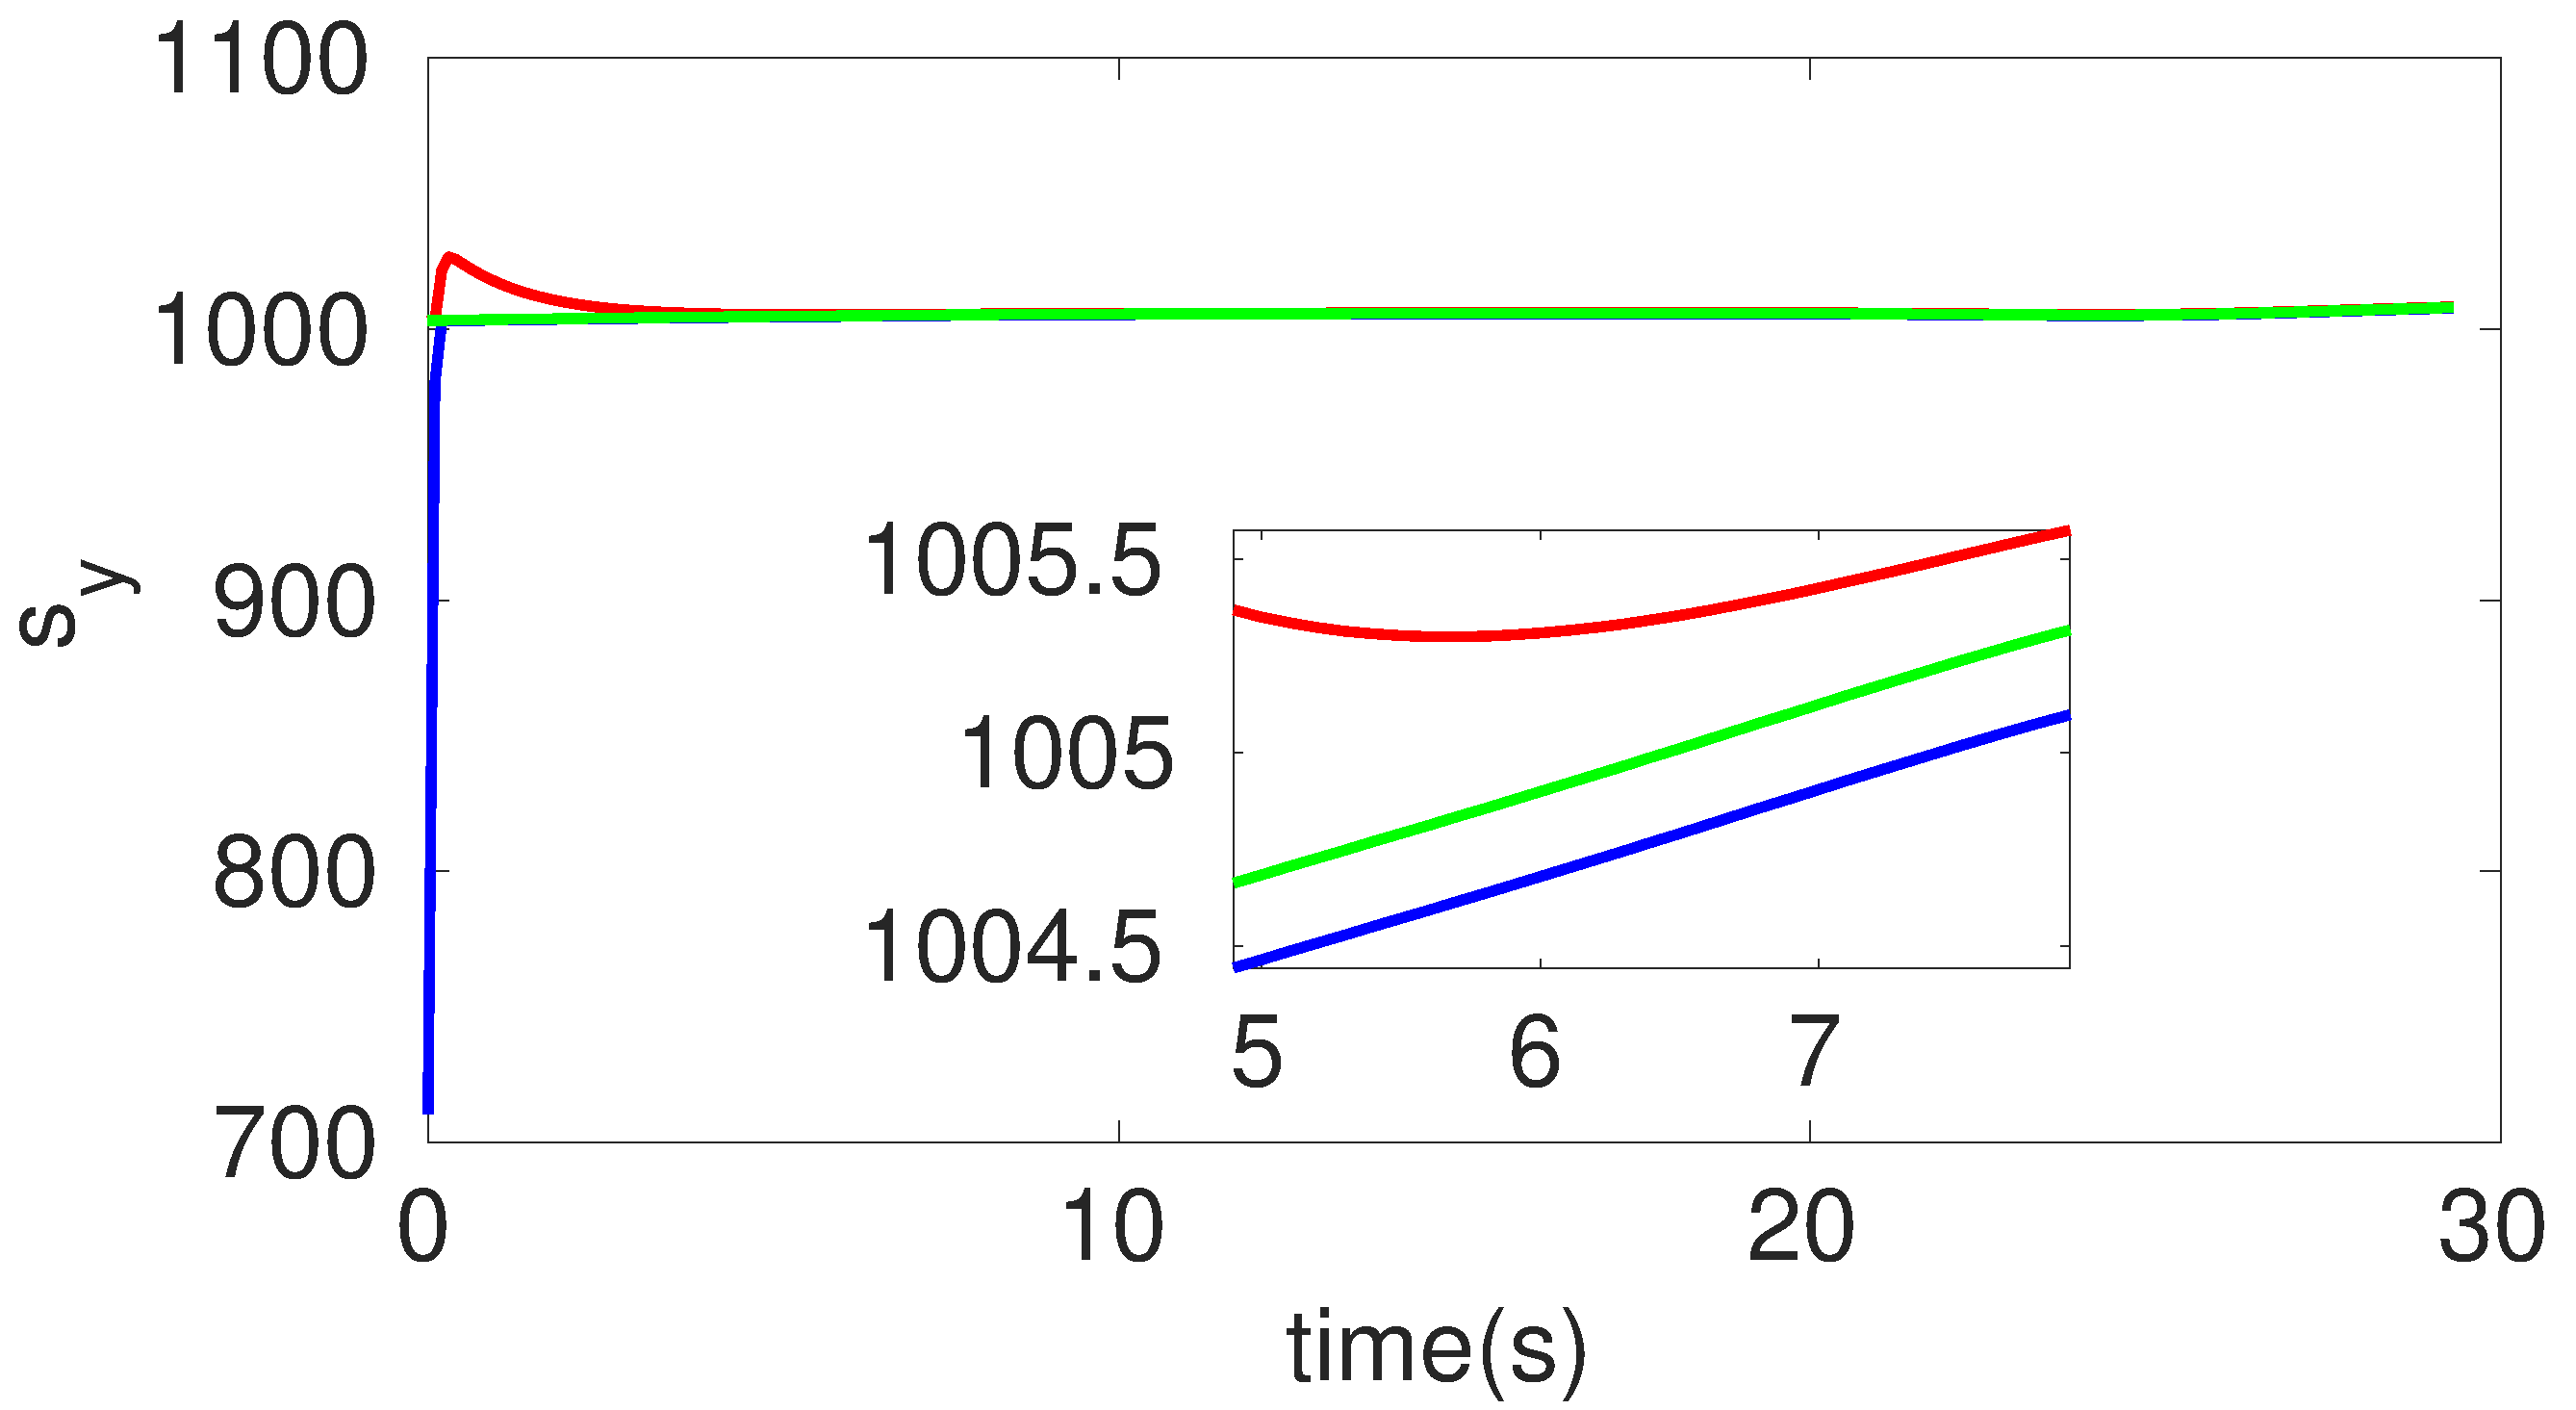
\includegraphics[width=\linewidth]{figures/Prad/s3cvprads_y}
\end{subfigure}
\begin{subfigure}{.5\linewidth}
\centering
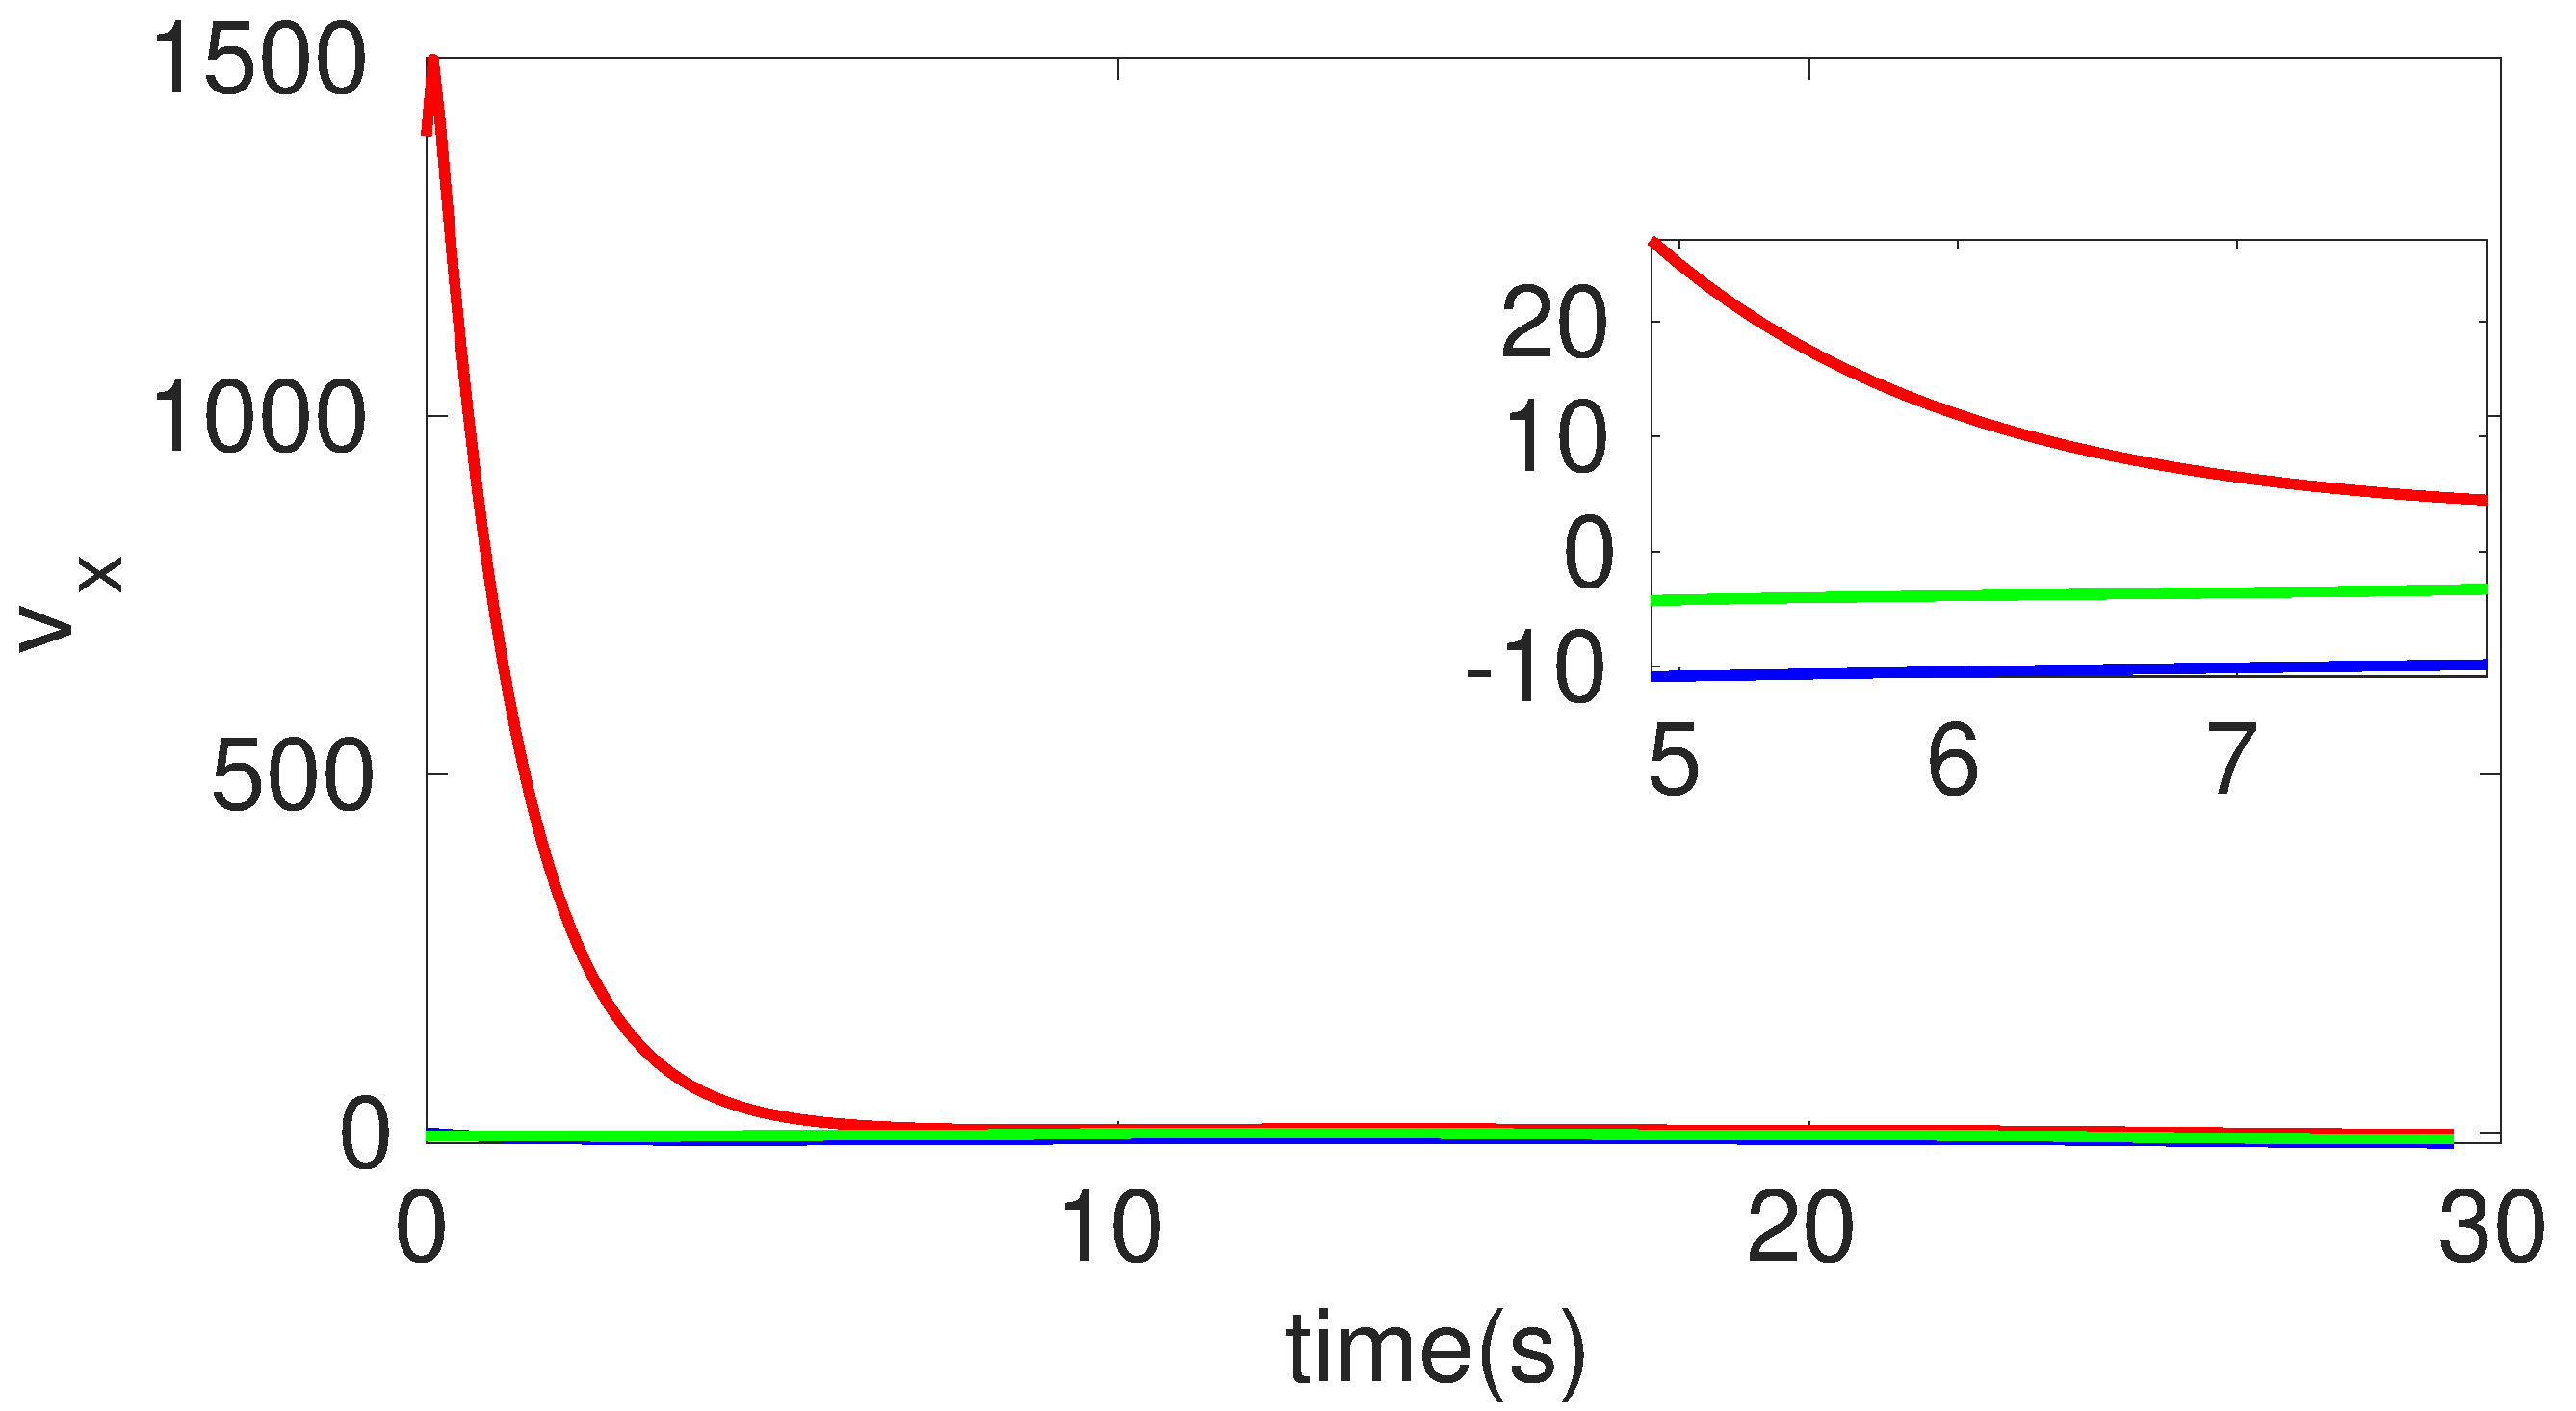
\includegraphics[width=\linewidth]{figures/Prad/s3cvpradv_x}
\end{subfigure}
\begin{subfigure}{.5\linewidth}
\centering
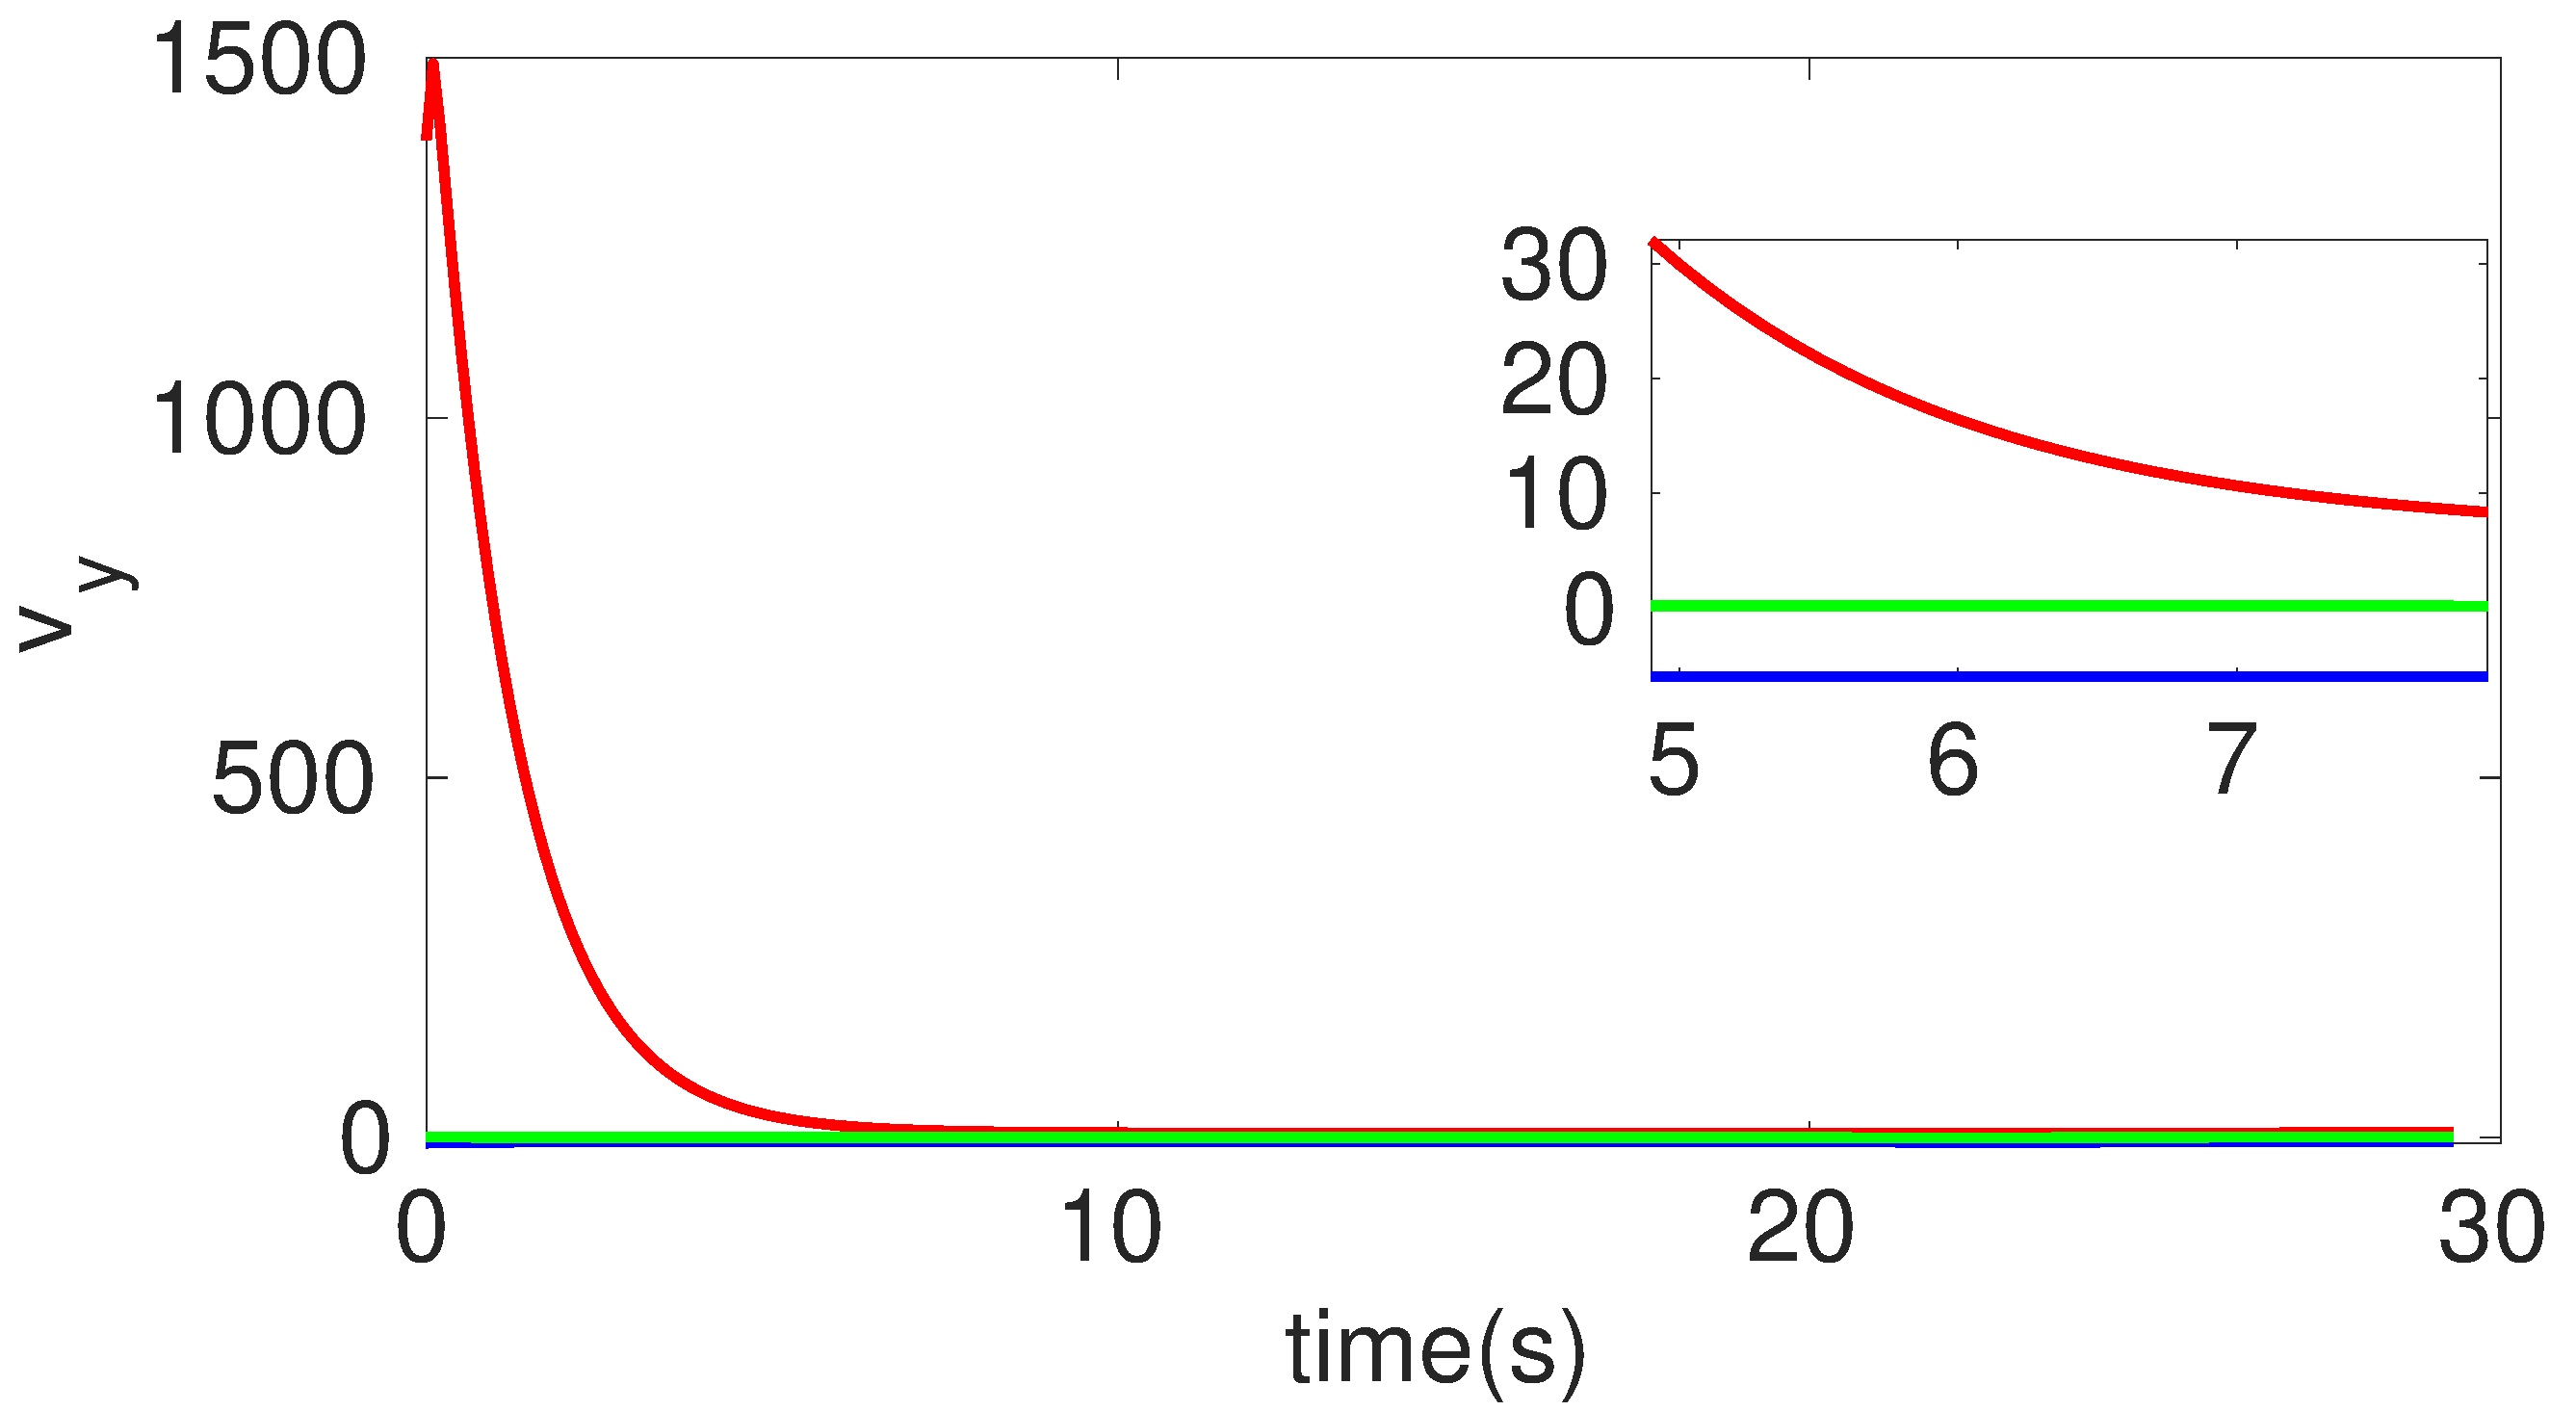
\includegraphics[width=\linewidth]{figures/Prad/s3cvpradv_y}
\end{subfigure}
\caption{Estimation using the P-radius minimizer and the constant velocity model}
\end{figure}

\begin{figure}[h]
\hspace*{\fill} 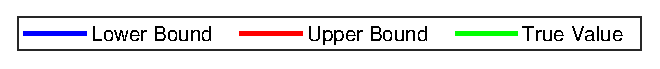
\includegraphics[scale=0.8]{figures/legend}\\\\
\begin{subfigure}{.5\linewidth}
\centering
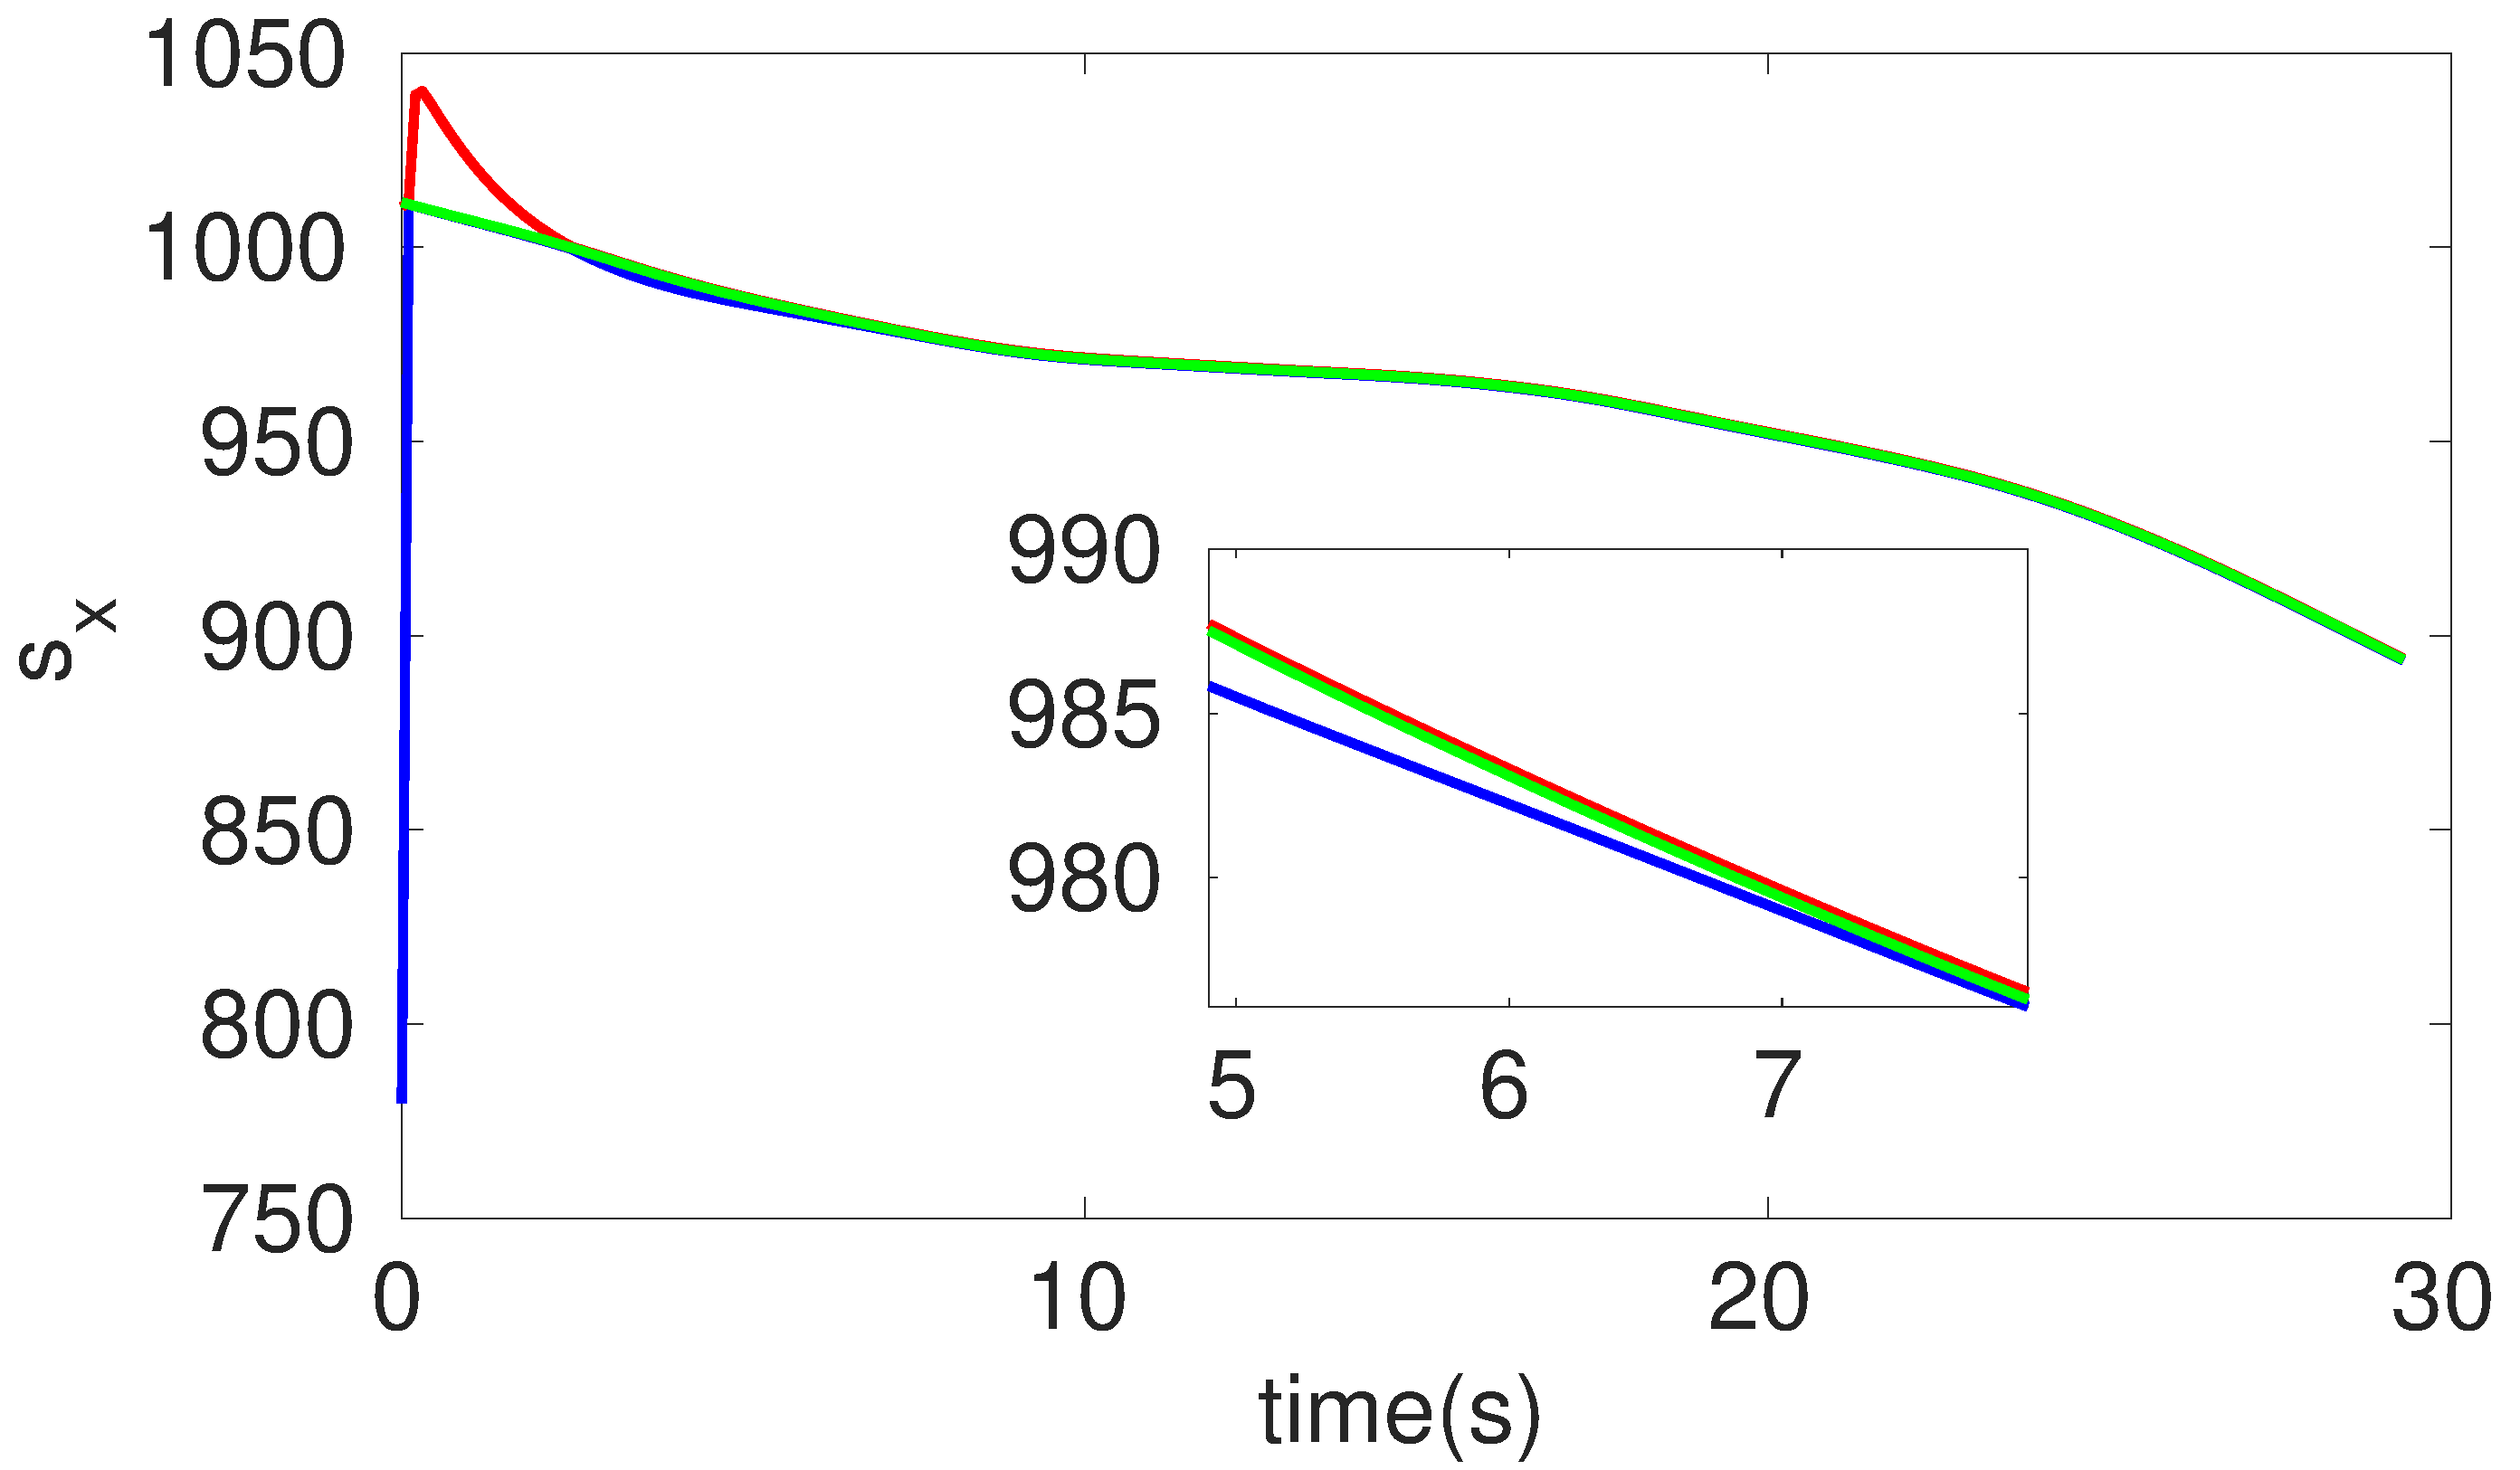
\includegraphics[width=\linewidth]{figures/Prad/s3caprads_x}
\end{subfigure}
\begin{subfigure}{.5\linewidth}
\centering
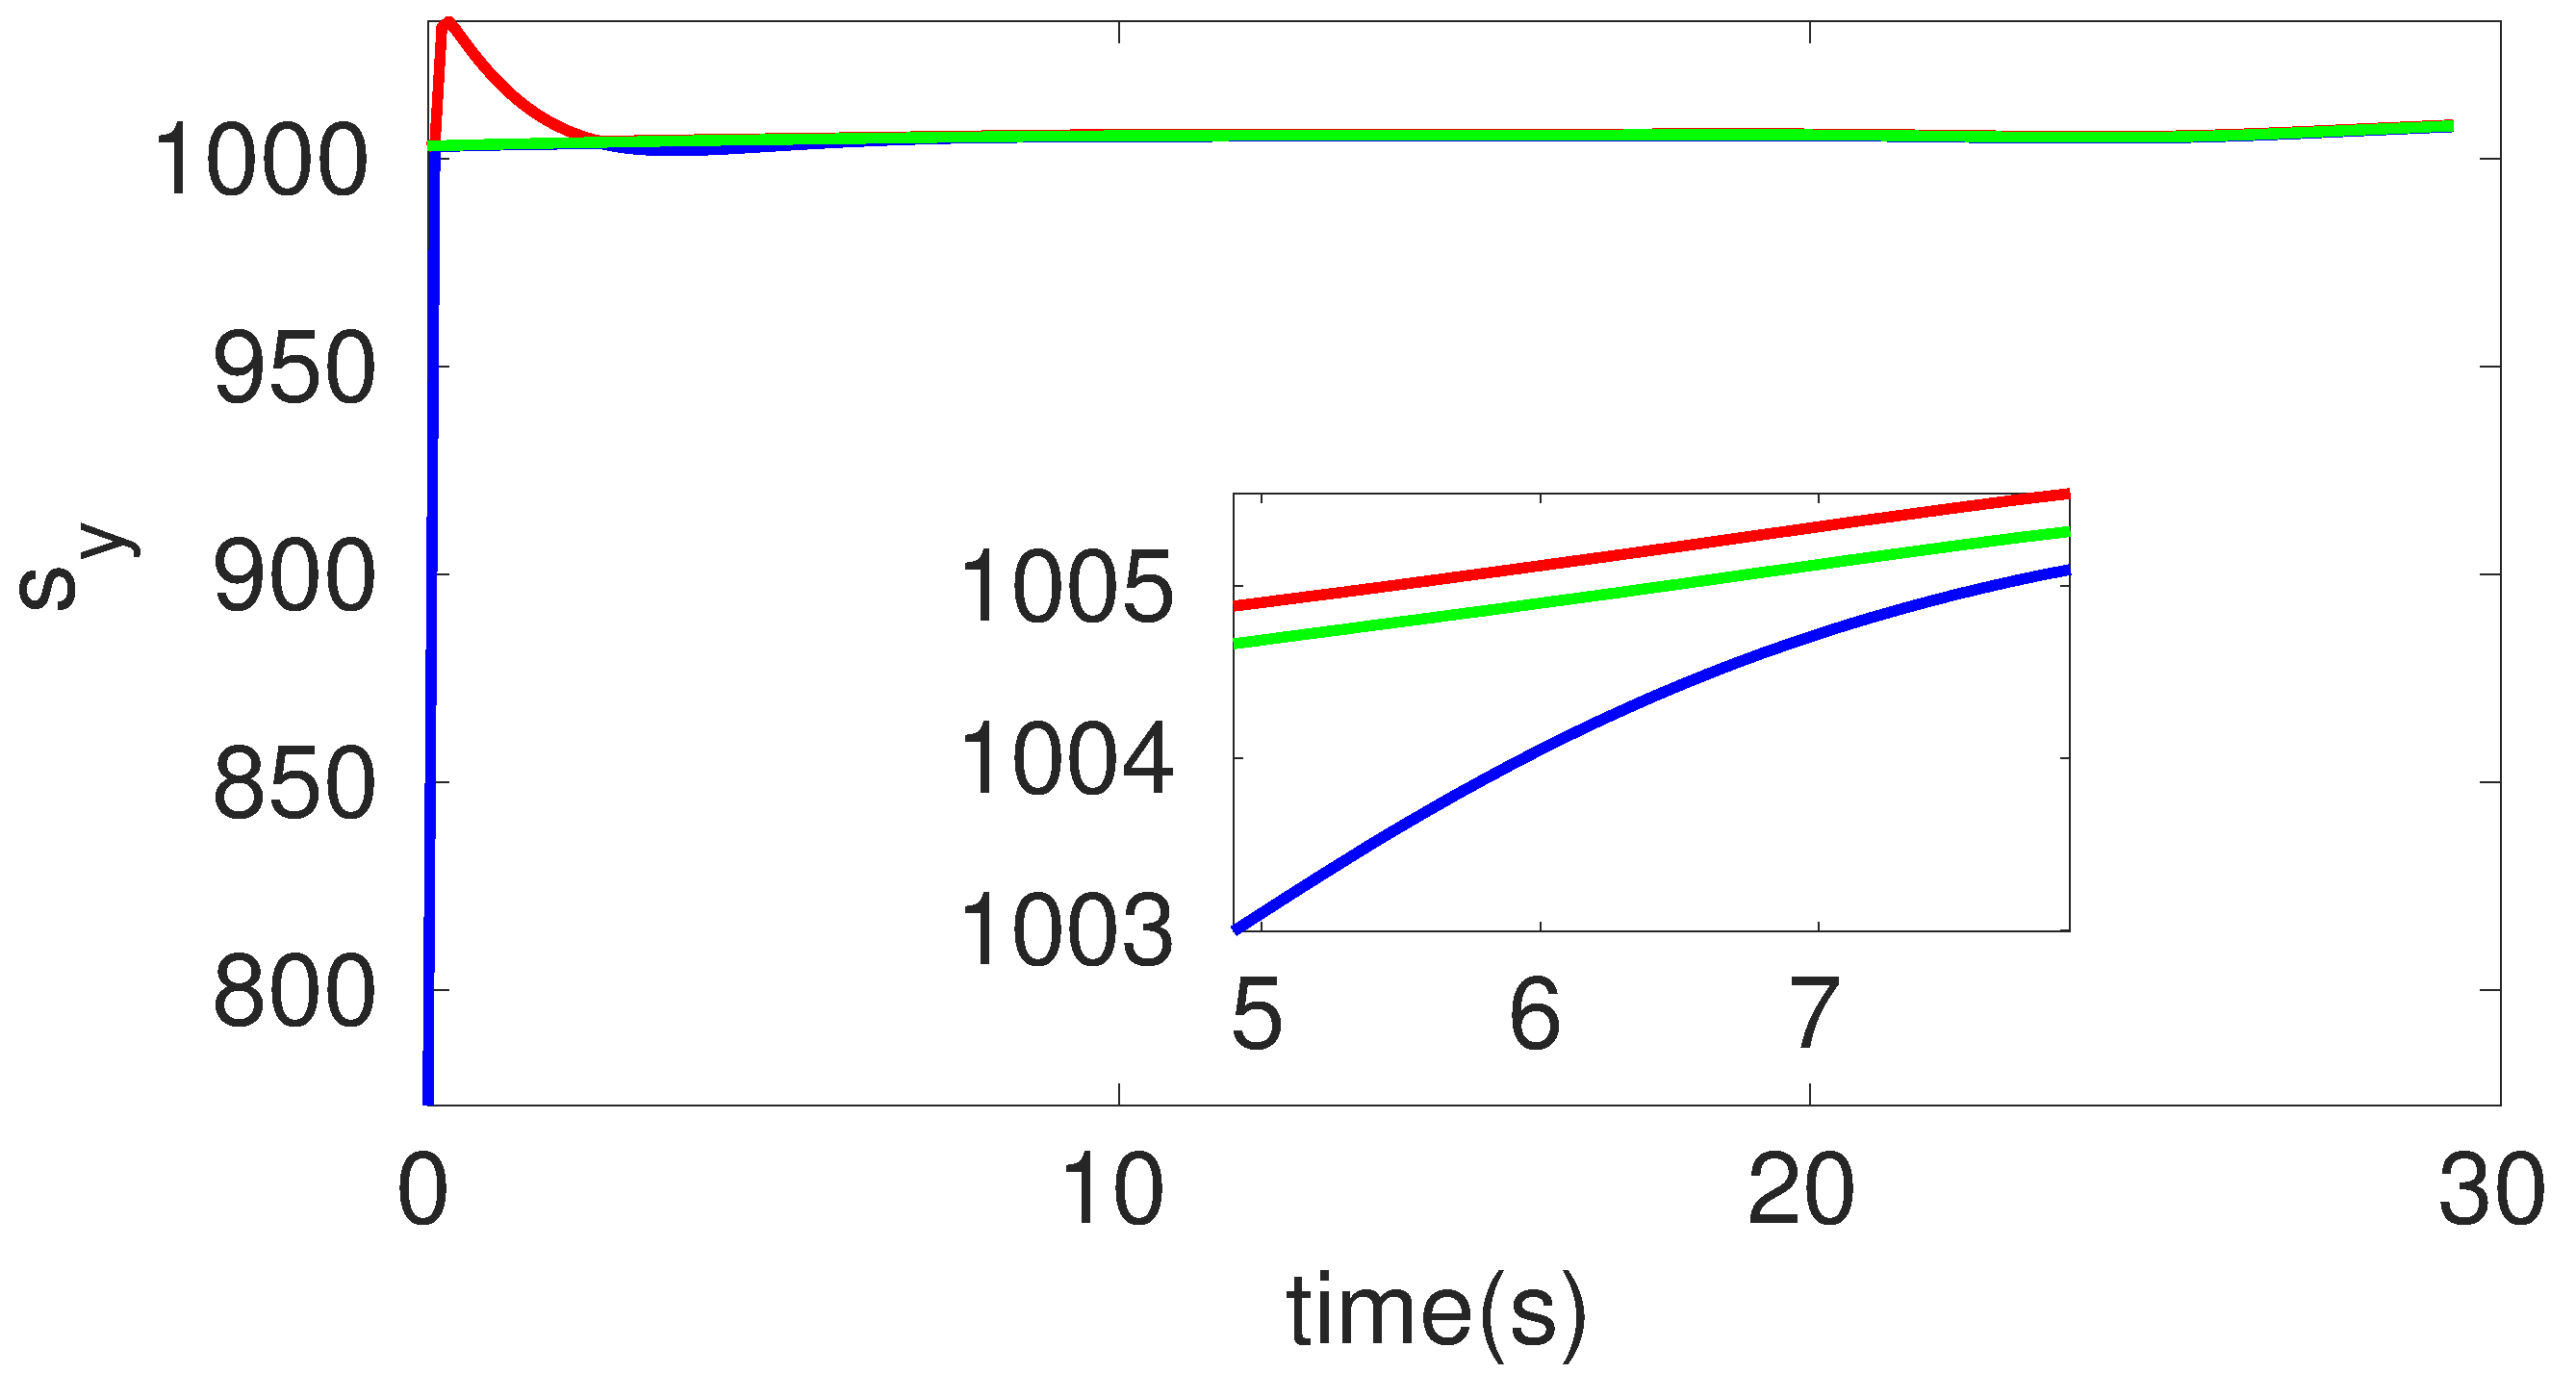
\includegraphics[width=\linewidth]{figures/Prad/s3caprads_y}
\end{subfigure}
\begin{subfigure}{.5\linewidth}
\centering
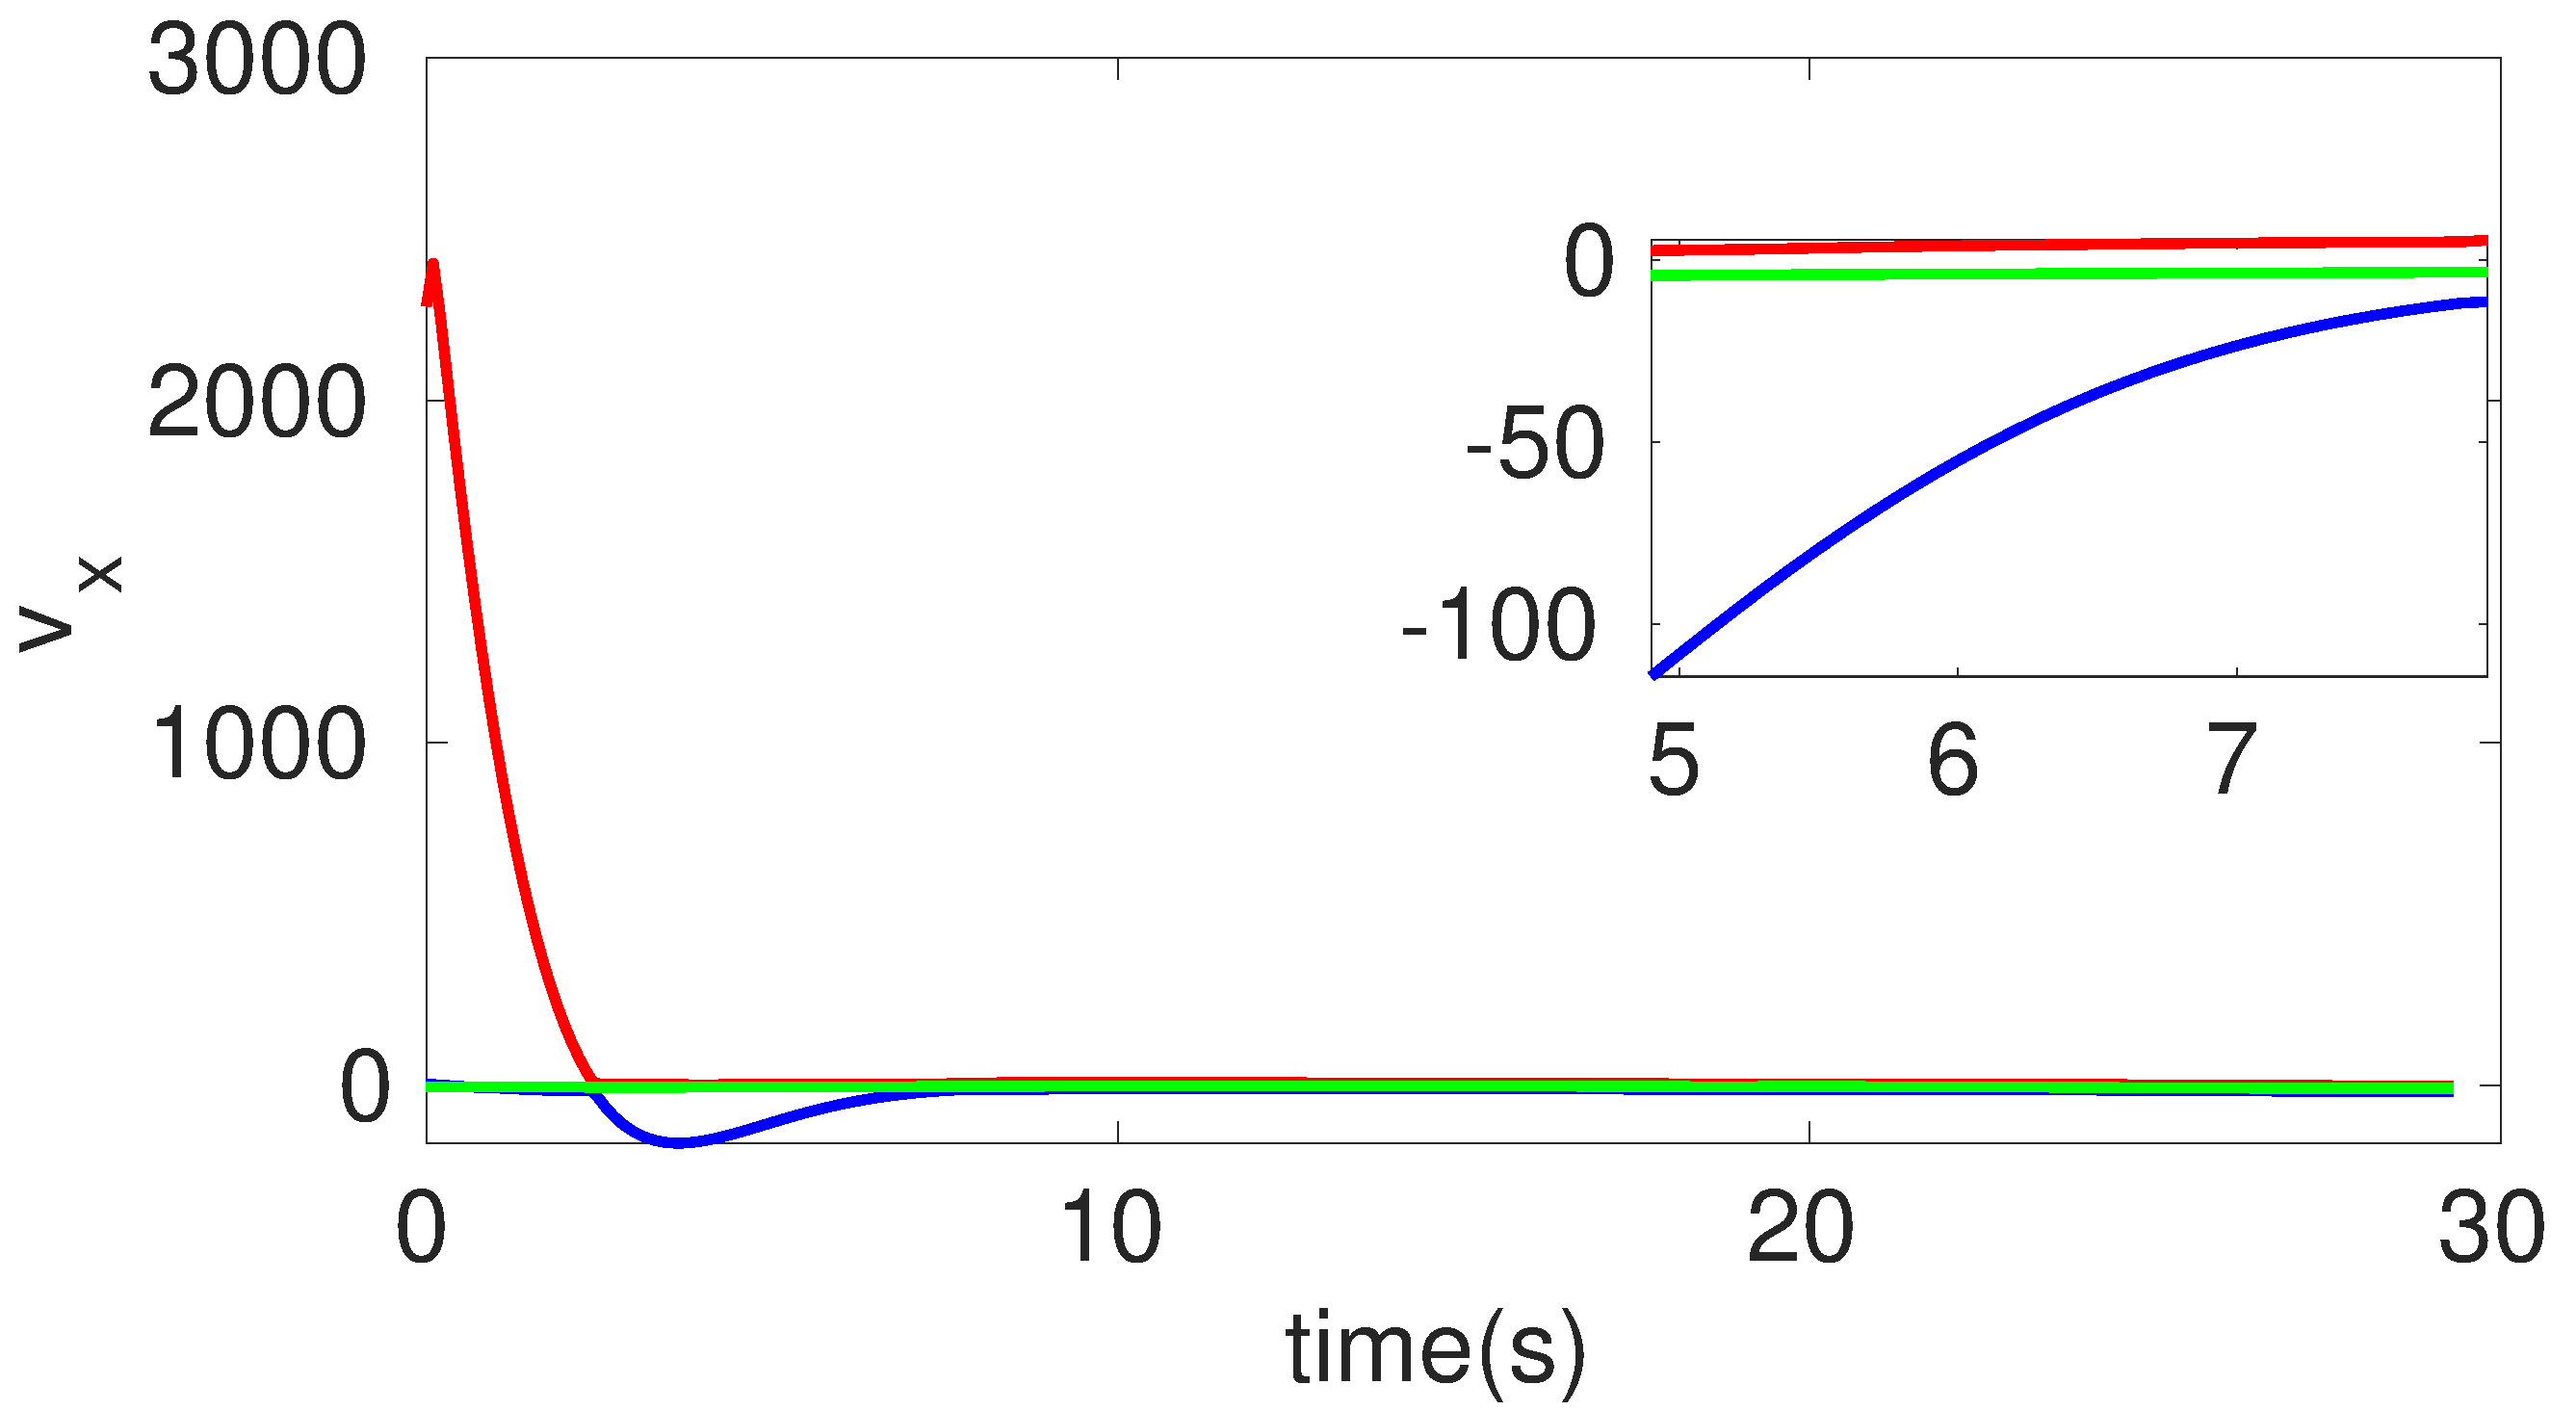
\includegraphics[width=\linewidth]{figures/Prad/s3capradv_x}
\end{subfigure}
\begin{subfigure}{.5\linewidth}
\centering
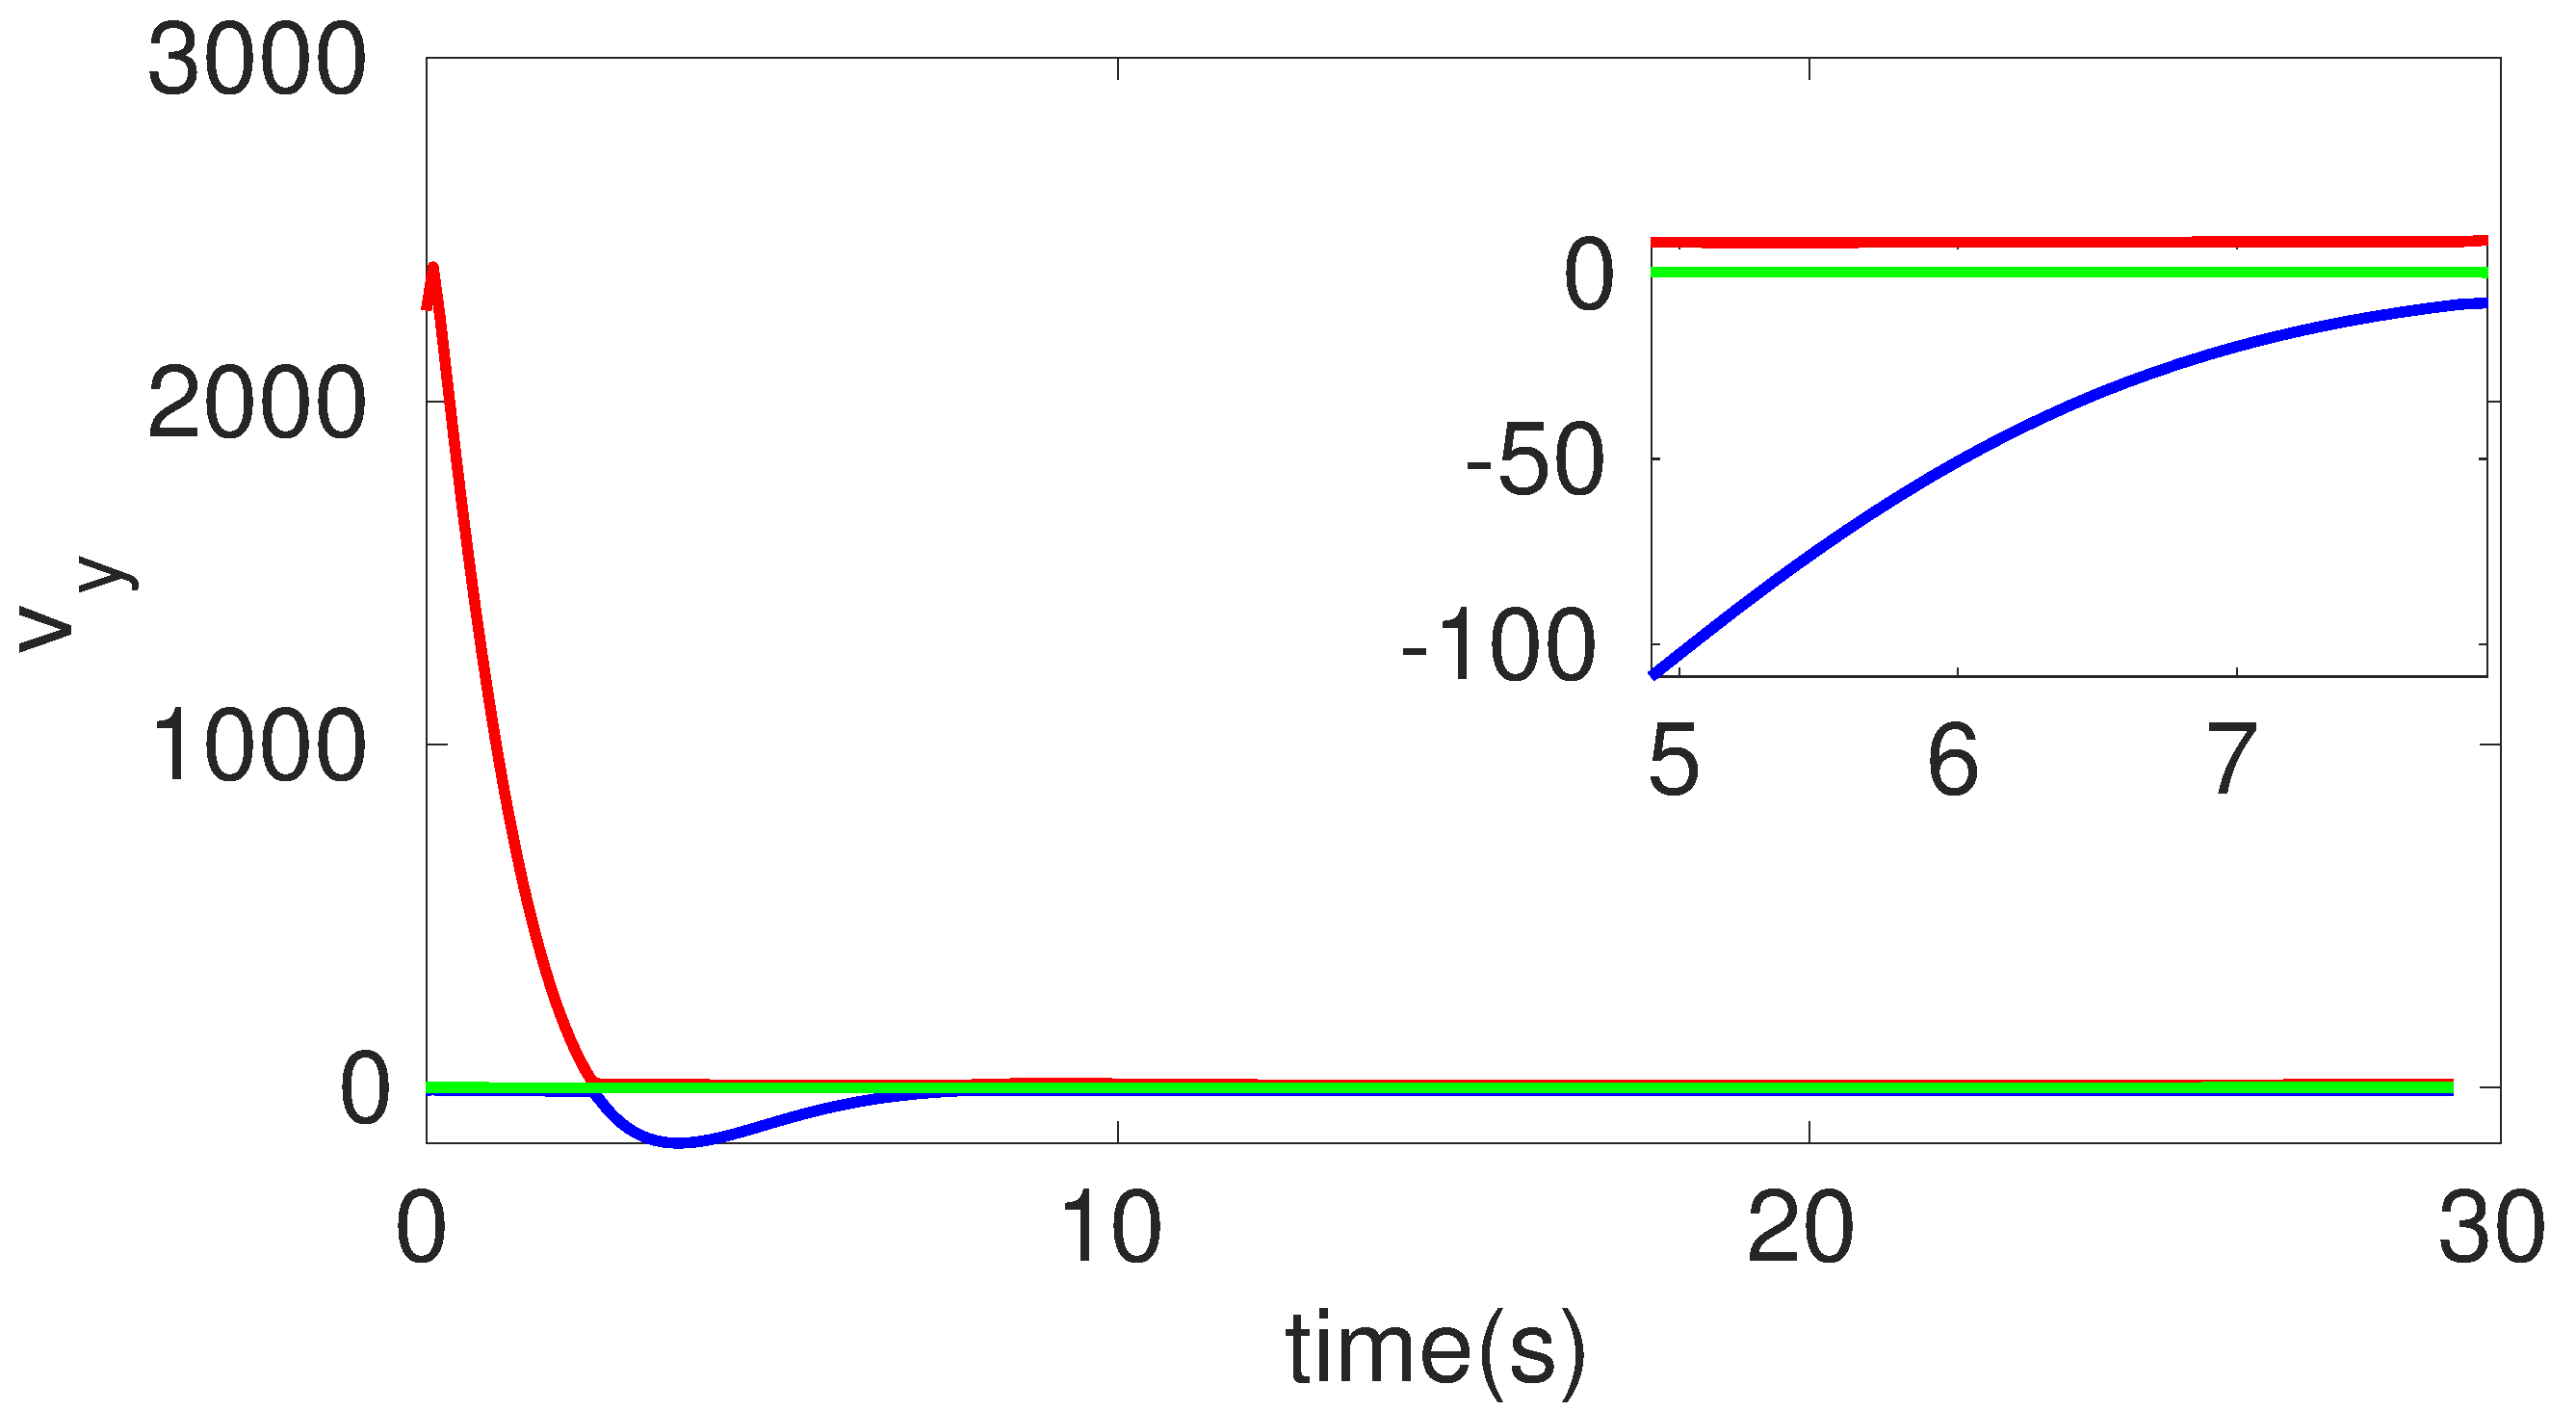
\includegraphics[width=\linewidth]{figures/Prad/s3capradv_y}
\end{subfigure}
\begin{subfigure}{.5\linewidth}
\centering
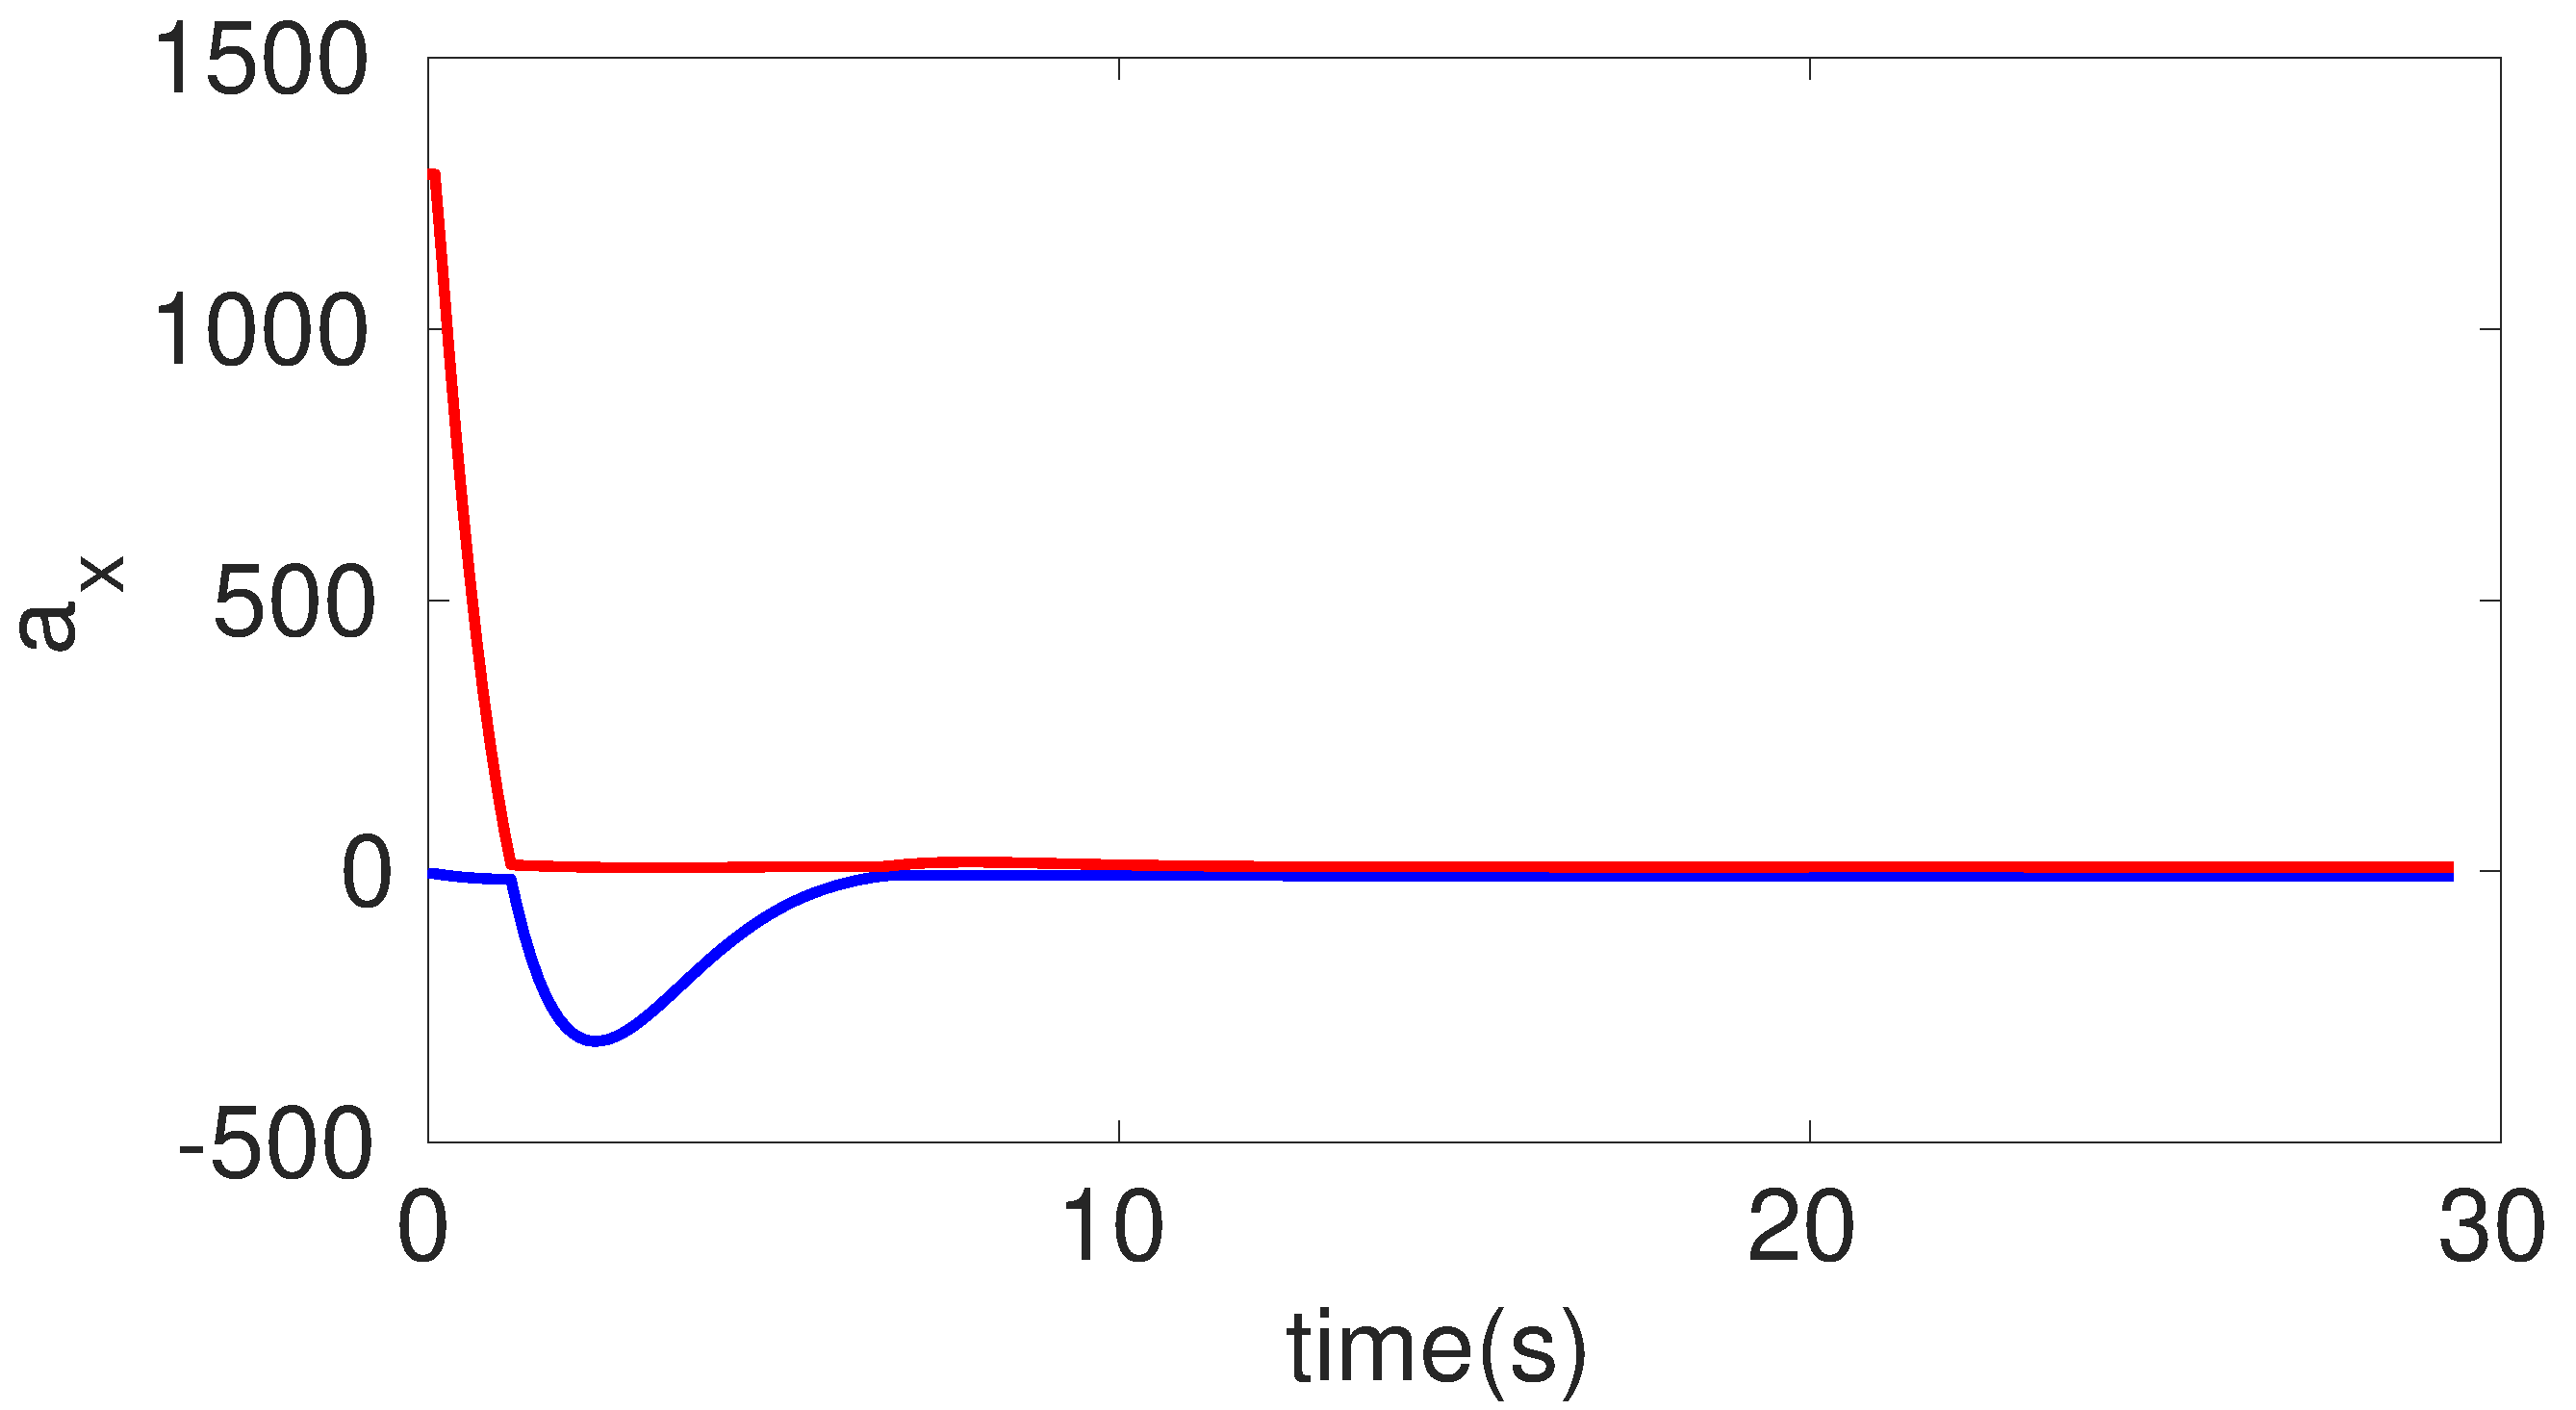
\includegraphics[width=\linewidth]{figures/Prad/s3caprada_x}
\end{subfigure}
\begin{subfigure}{.5\linewidth}
\centering
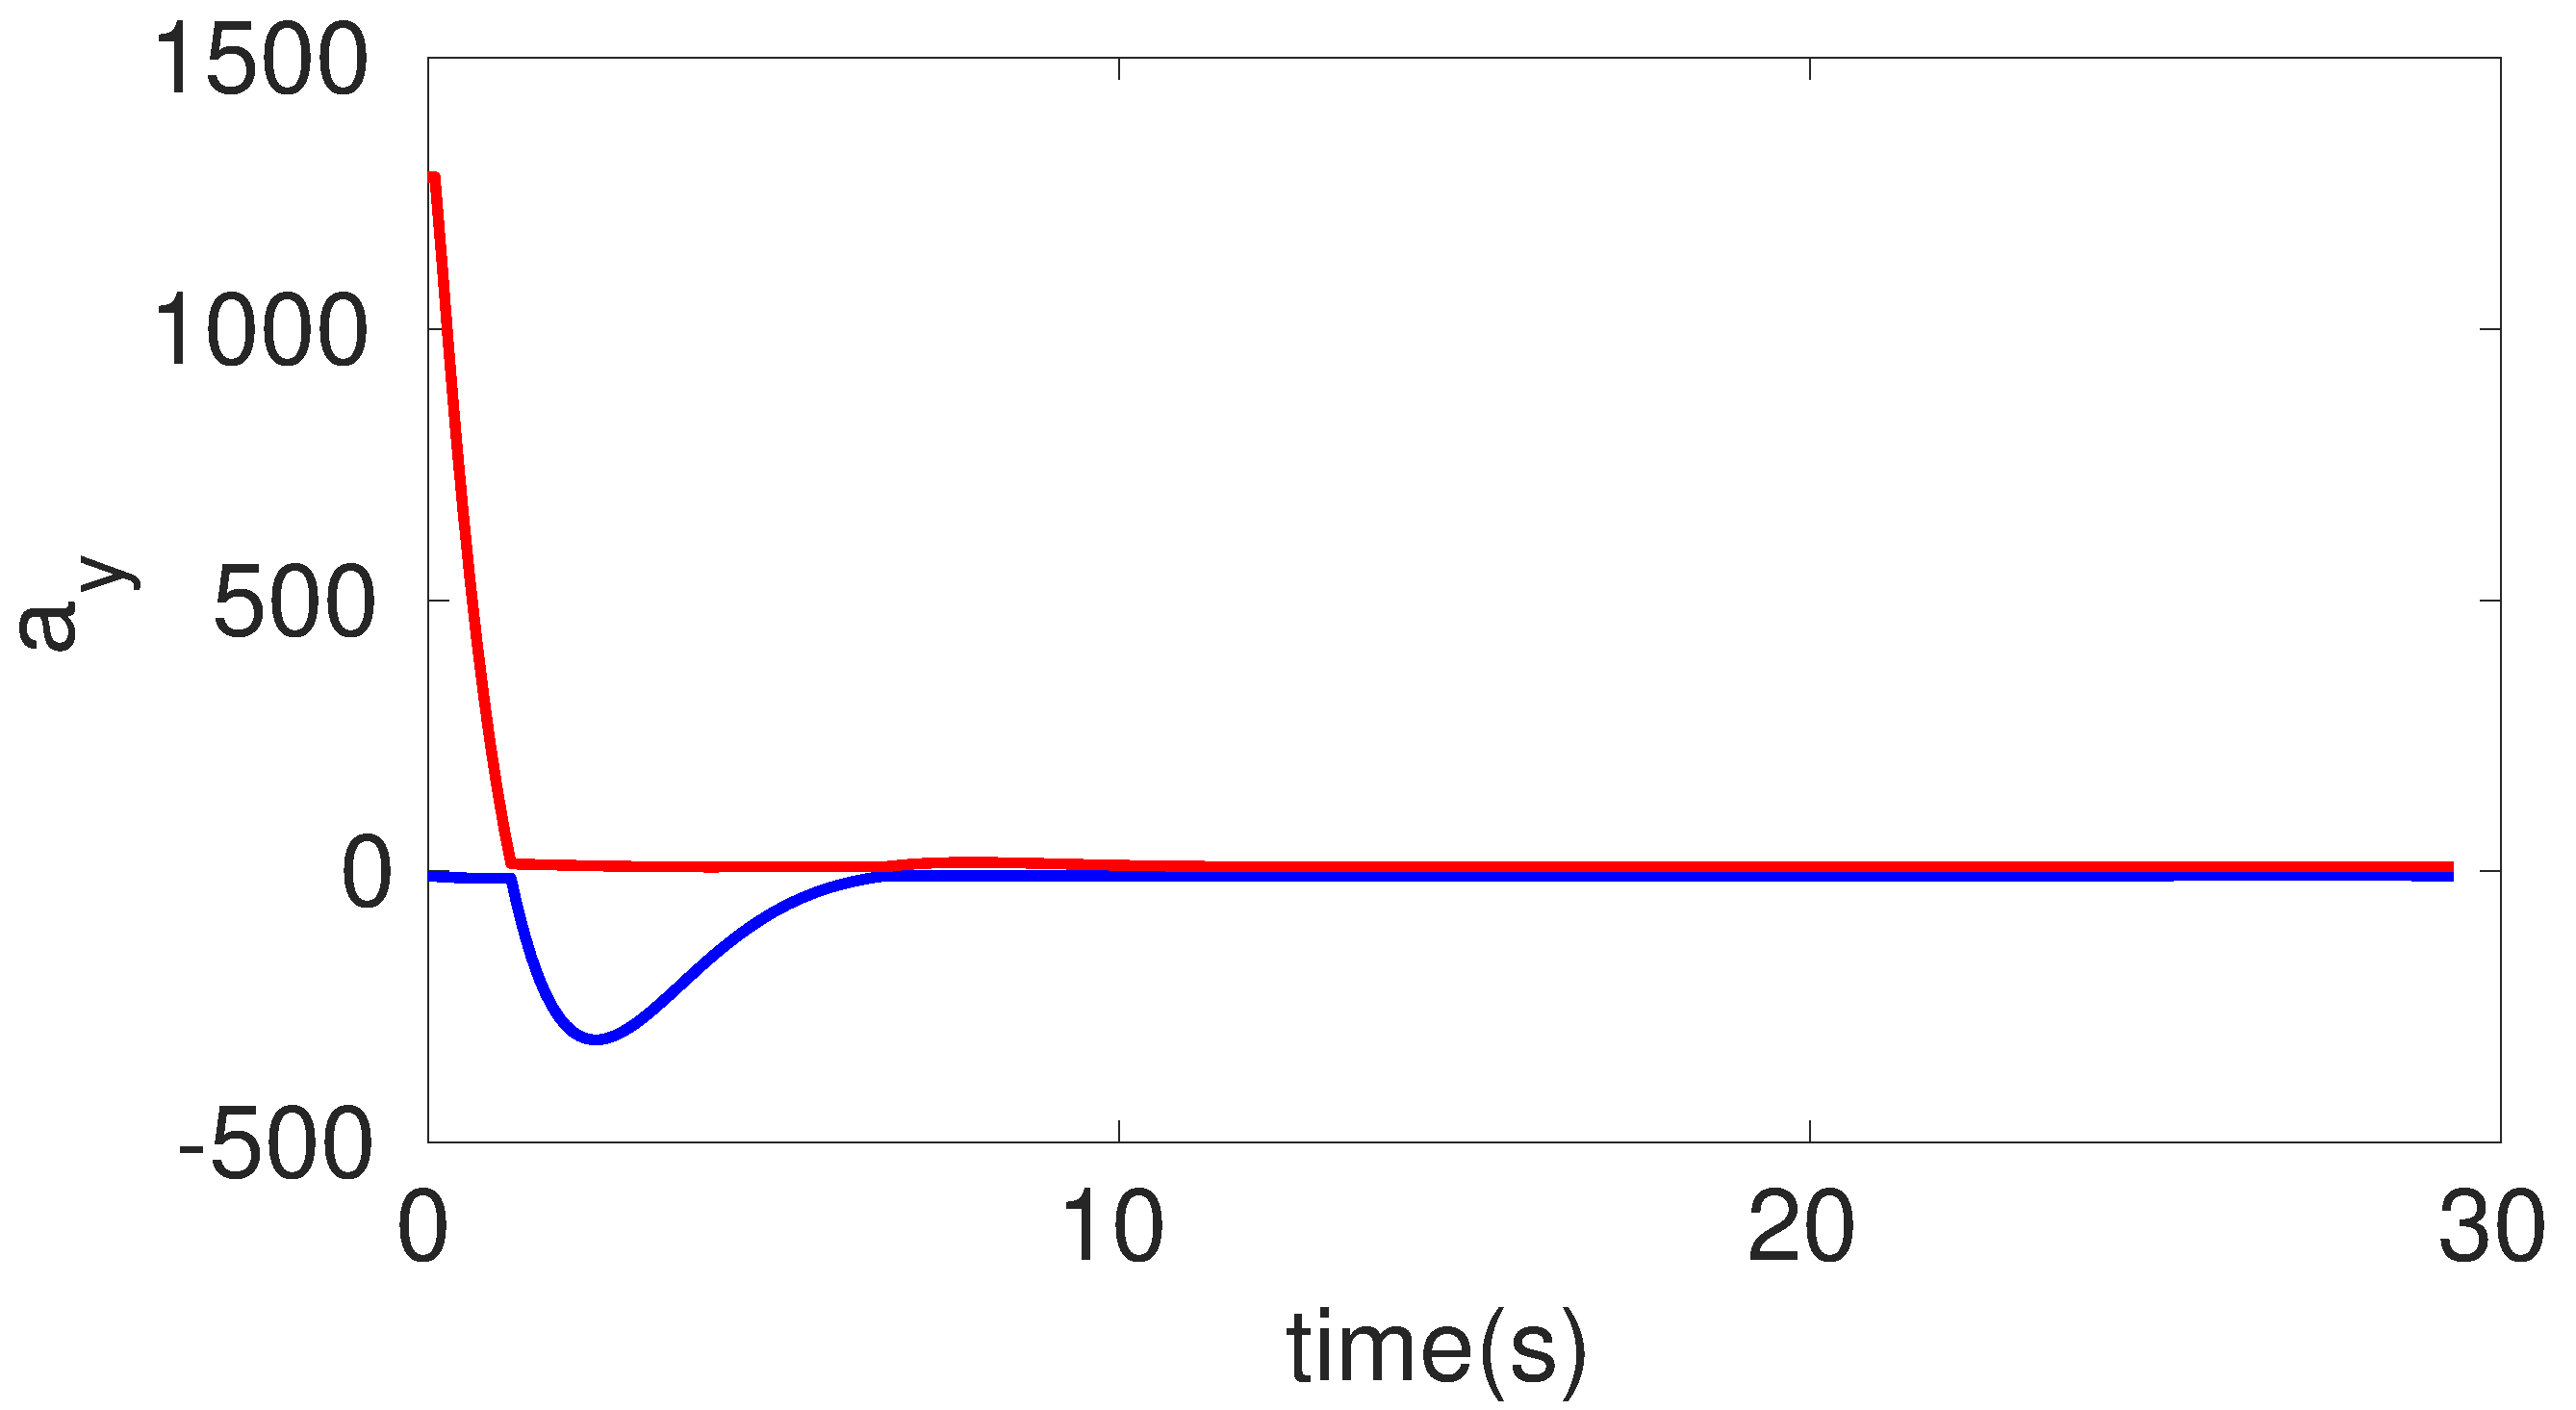
\includegraphics[width=\linewidth]{figures/Prad/s3caprada_y}
\end{subfigure}
\caption{Estimation using the P-radius minimizer and the constant acceleration model}
\end{figure}

\begin{figure}[h]
\hspace*{\fill} 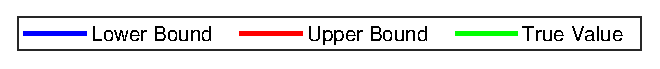
\includegraphics[scale=0.8]{figures/legend}\\\\
\begin{subfigure}{.5\linewidth}
\centering
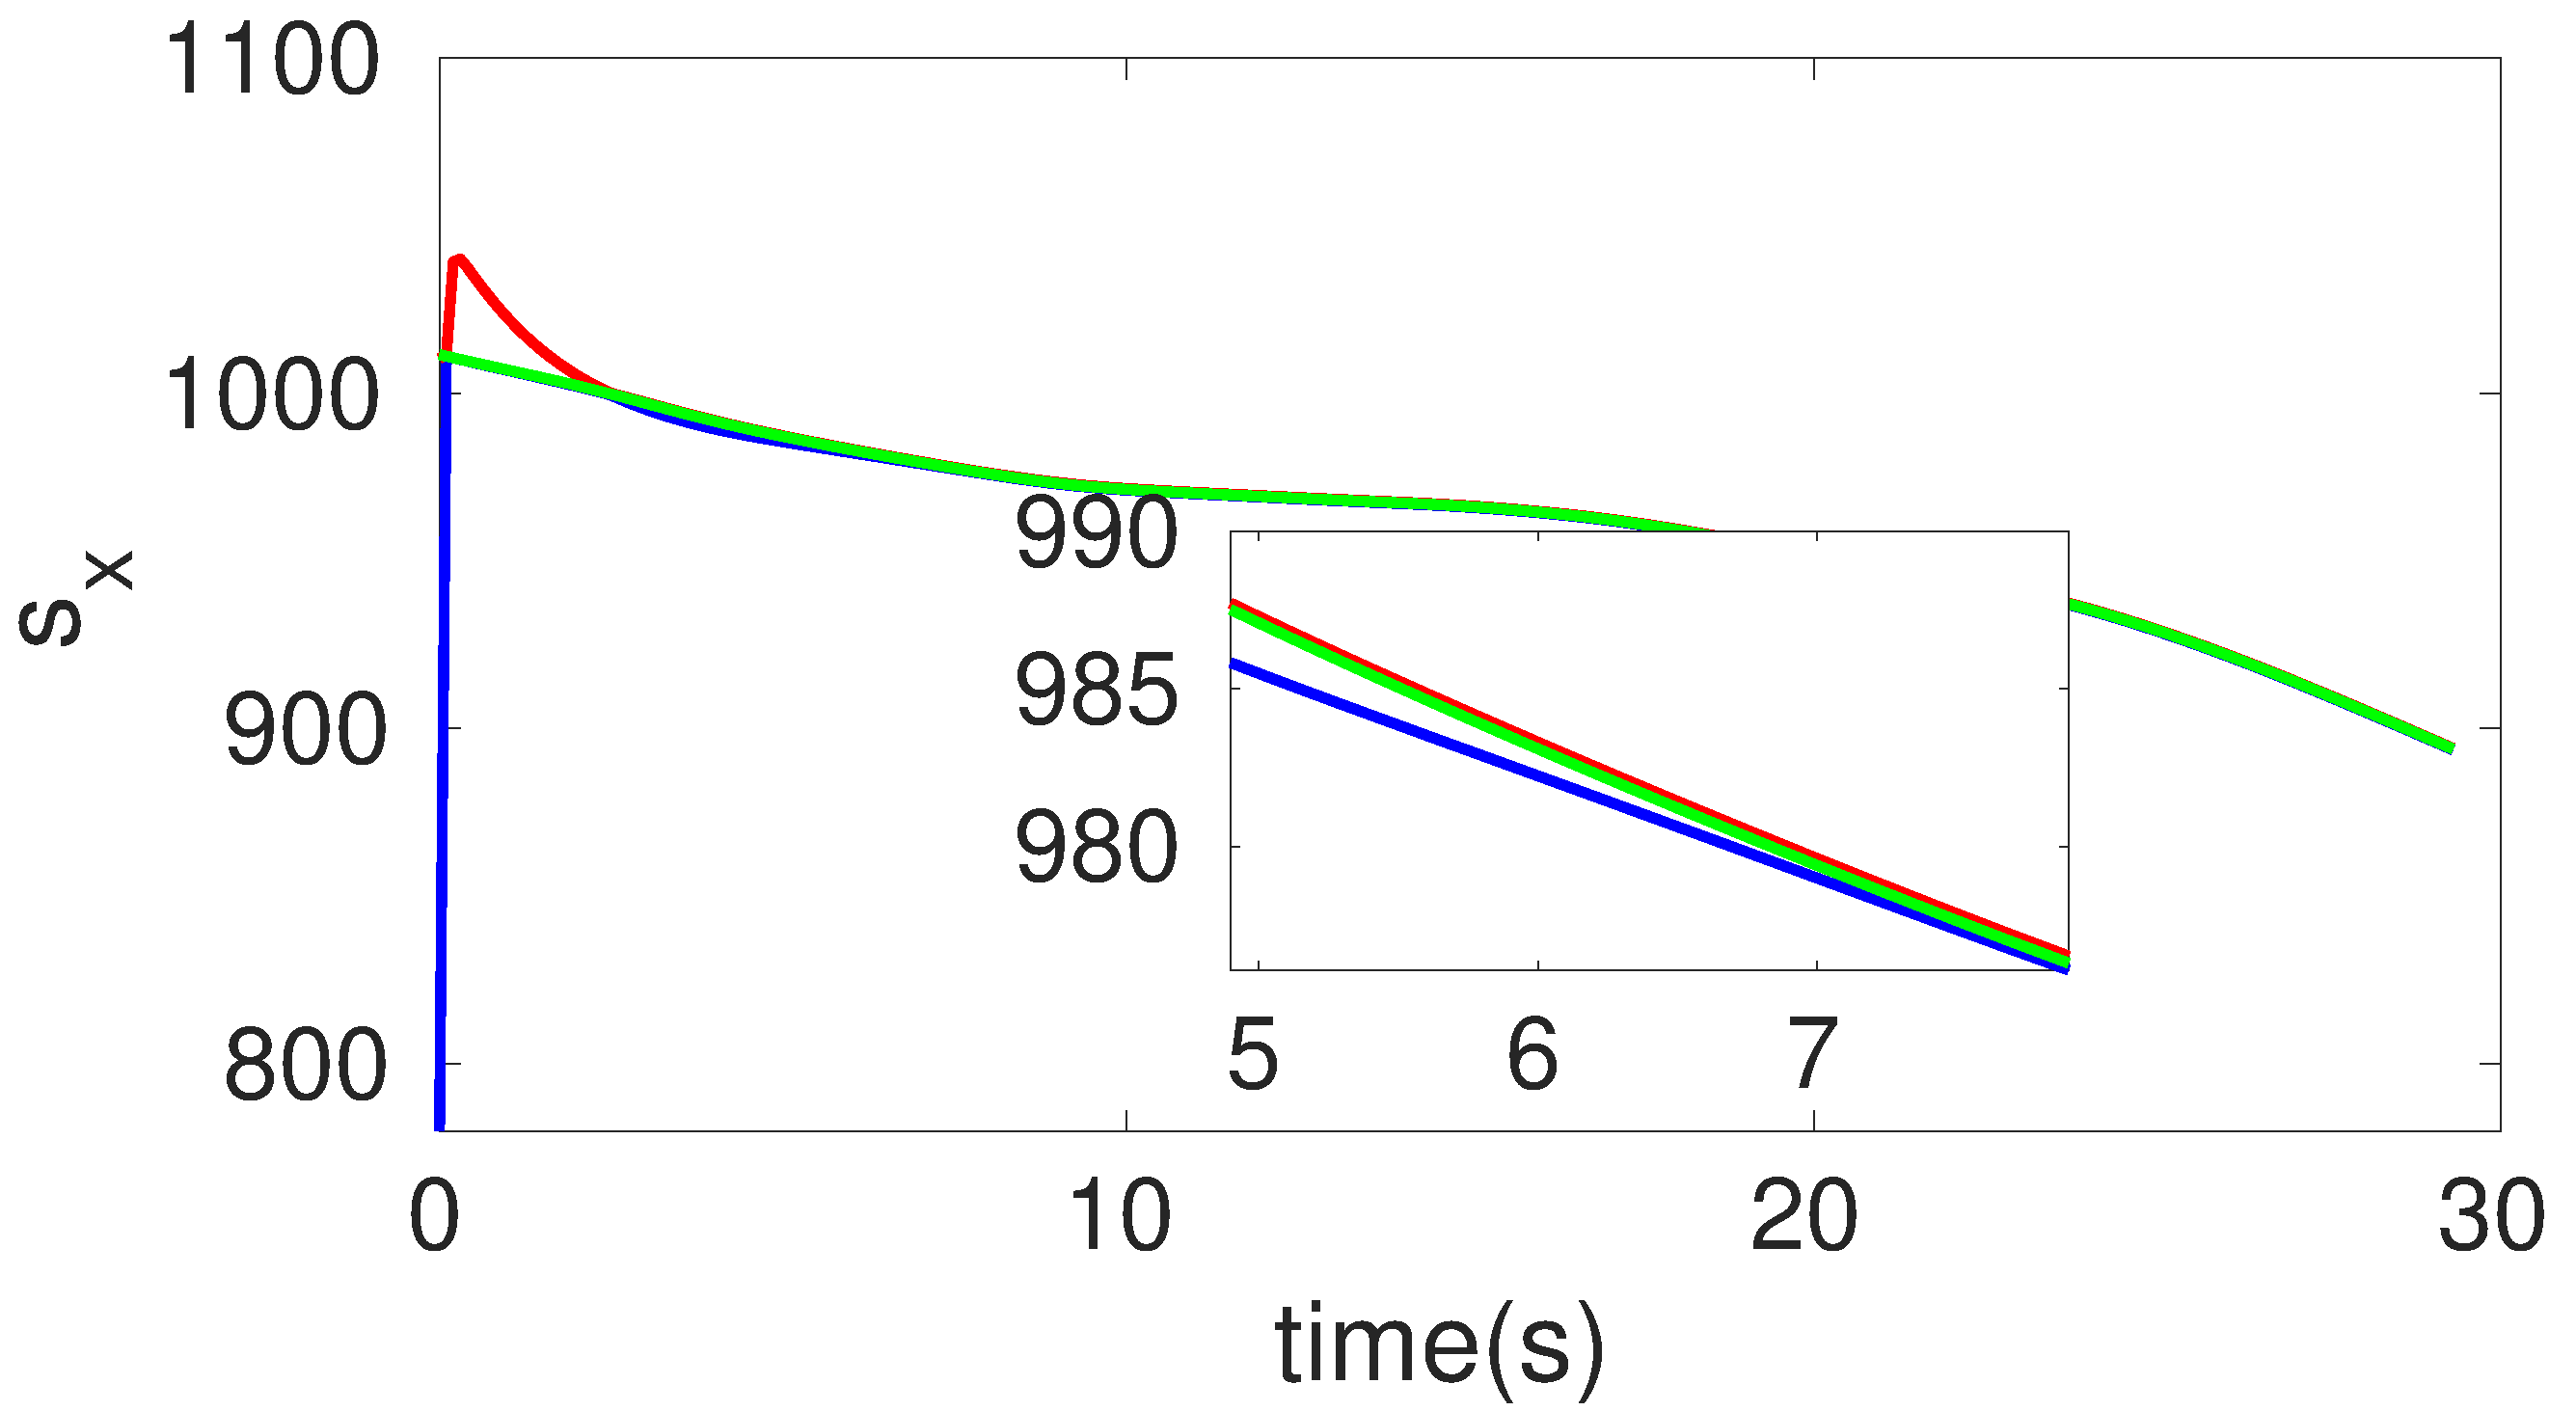
\includegraphics[width=\linewidth]{figures/Prad/s3pmprads_x}
\end{subfigure}
\begin{subfigure}{.5\linewidth}
\centering
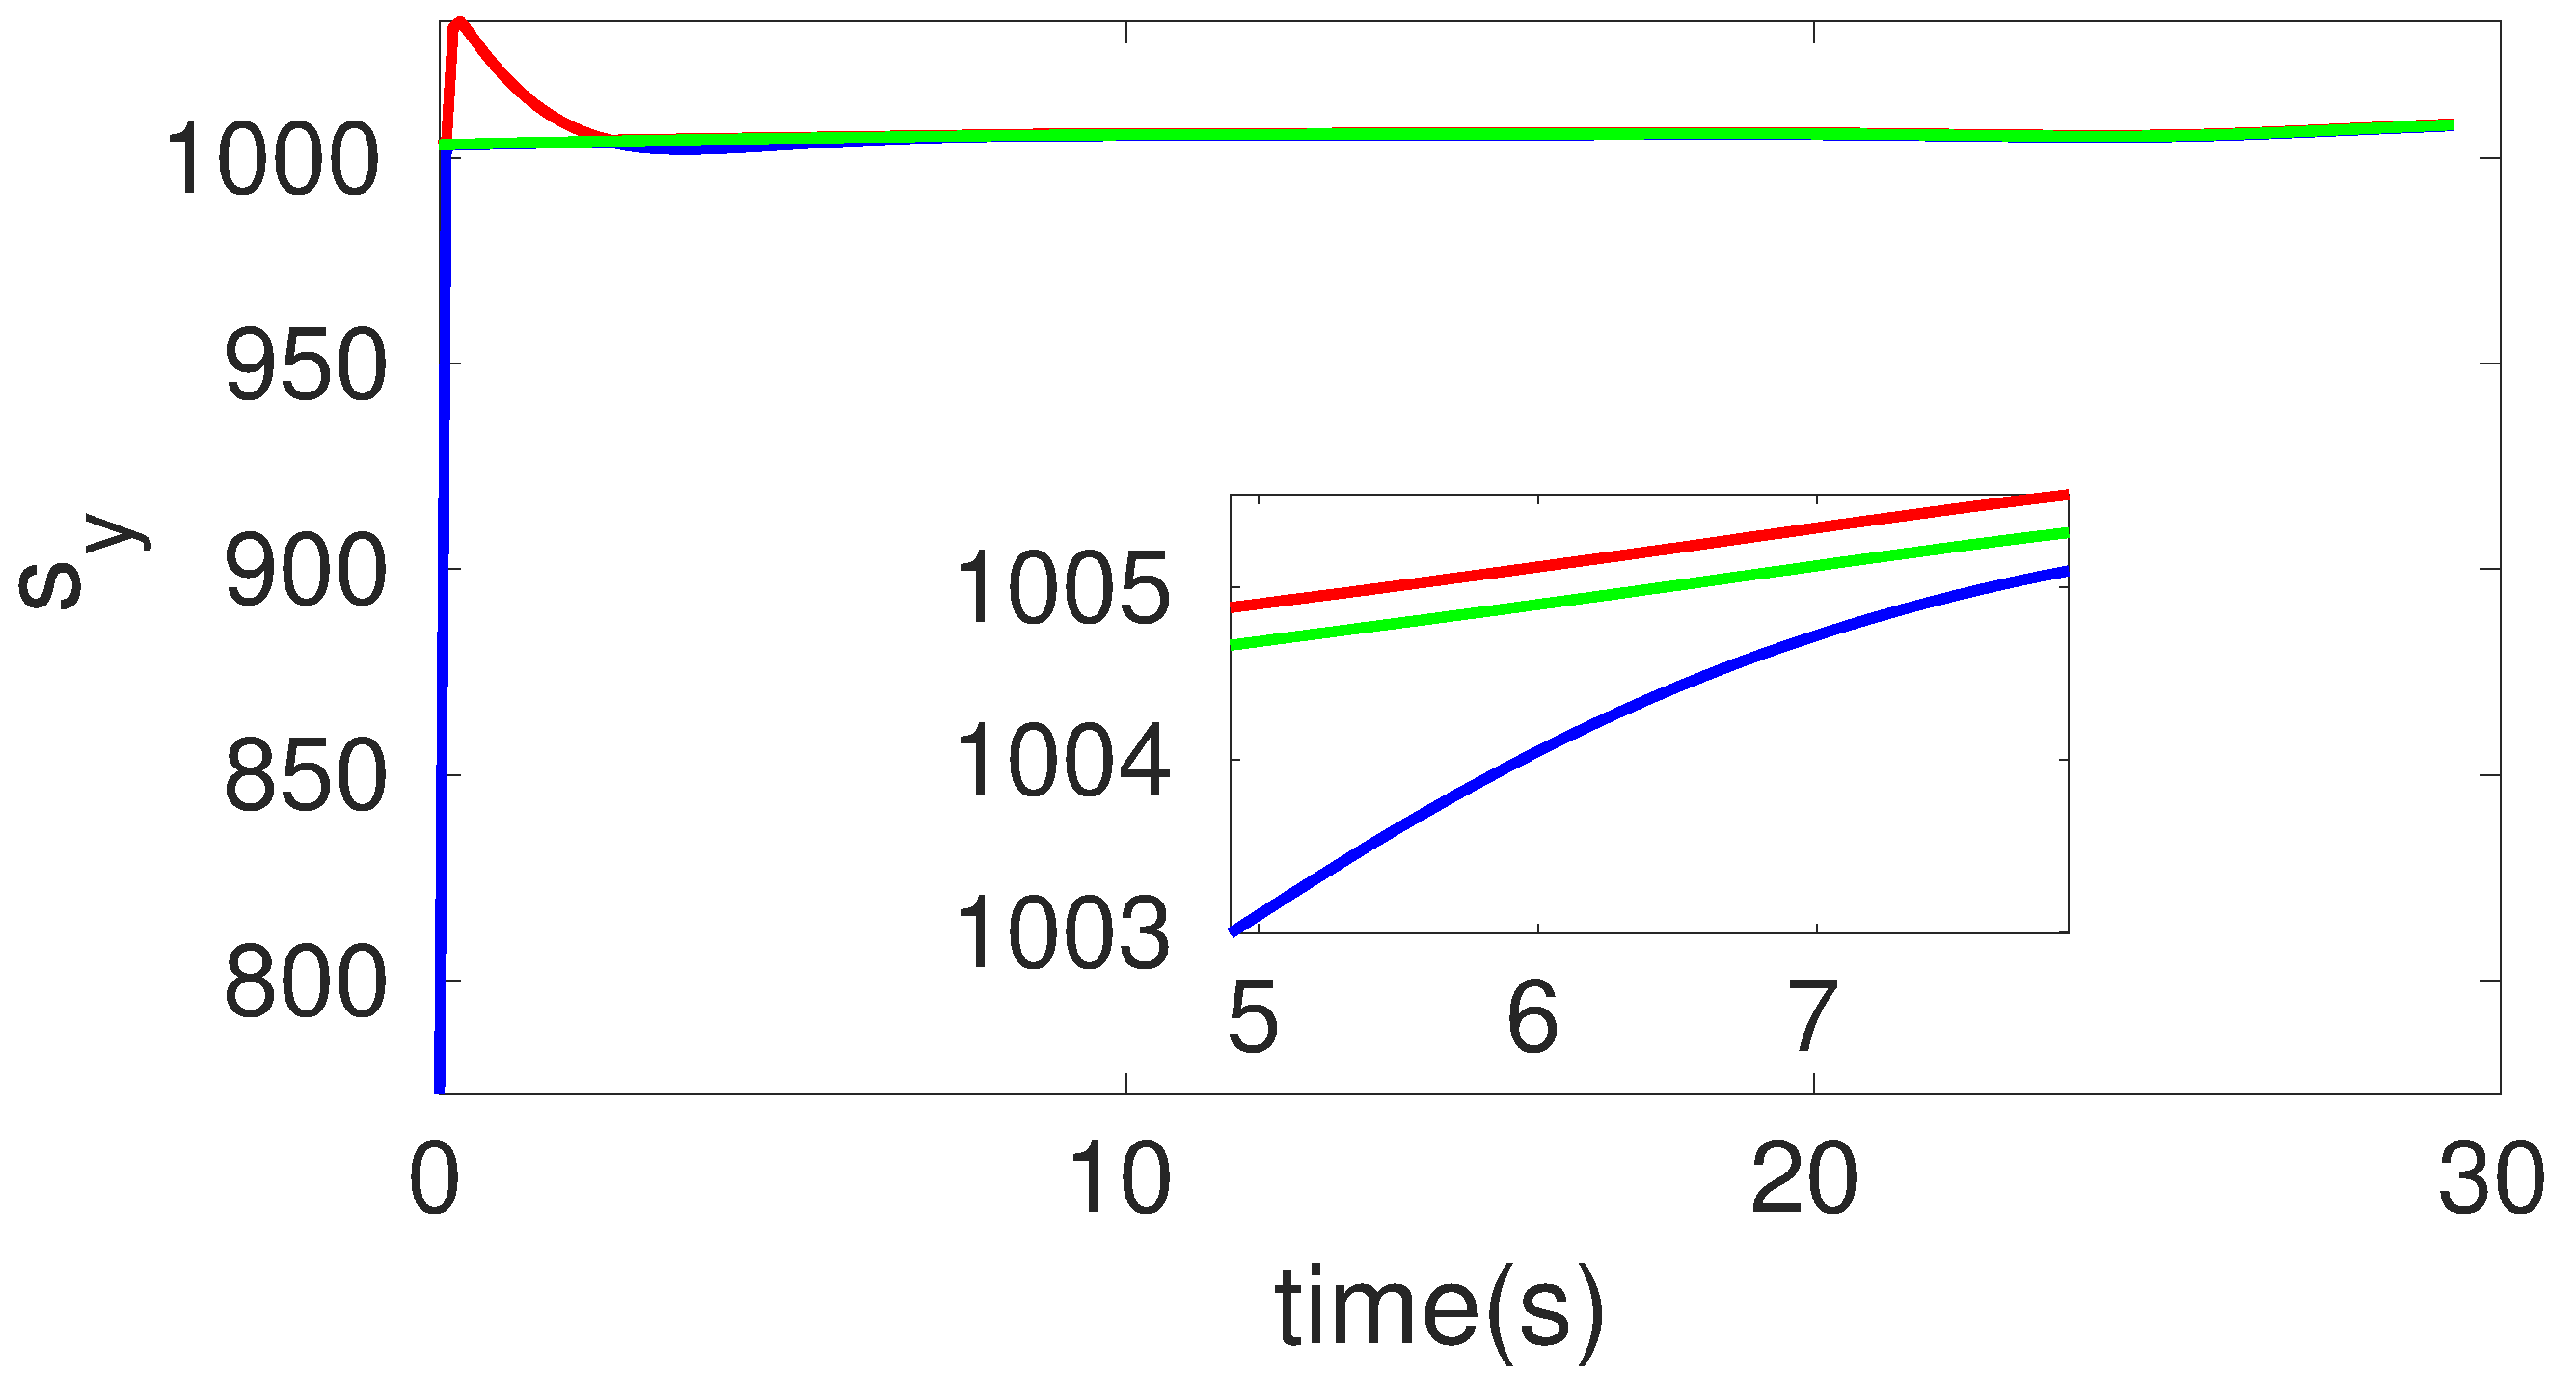
\includegraphics[width=\linewidth]{figures/Prad/s3pmprads_y}
\end{subfigure}
\begin{subfigure}{.5\linewidth}
\centering
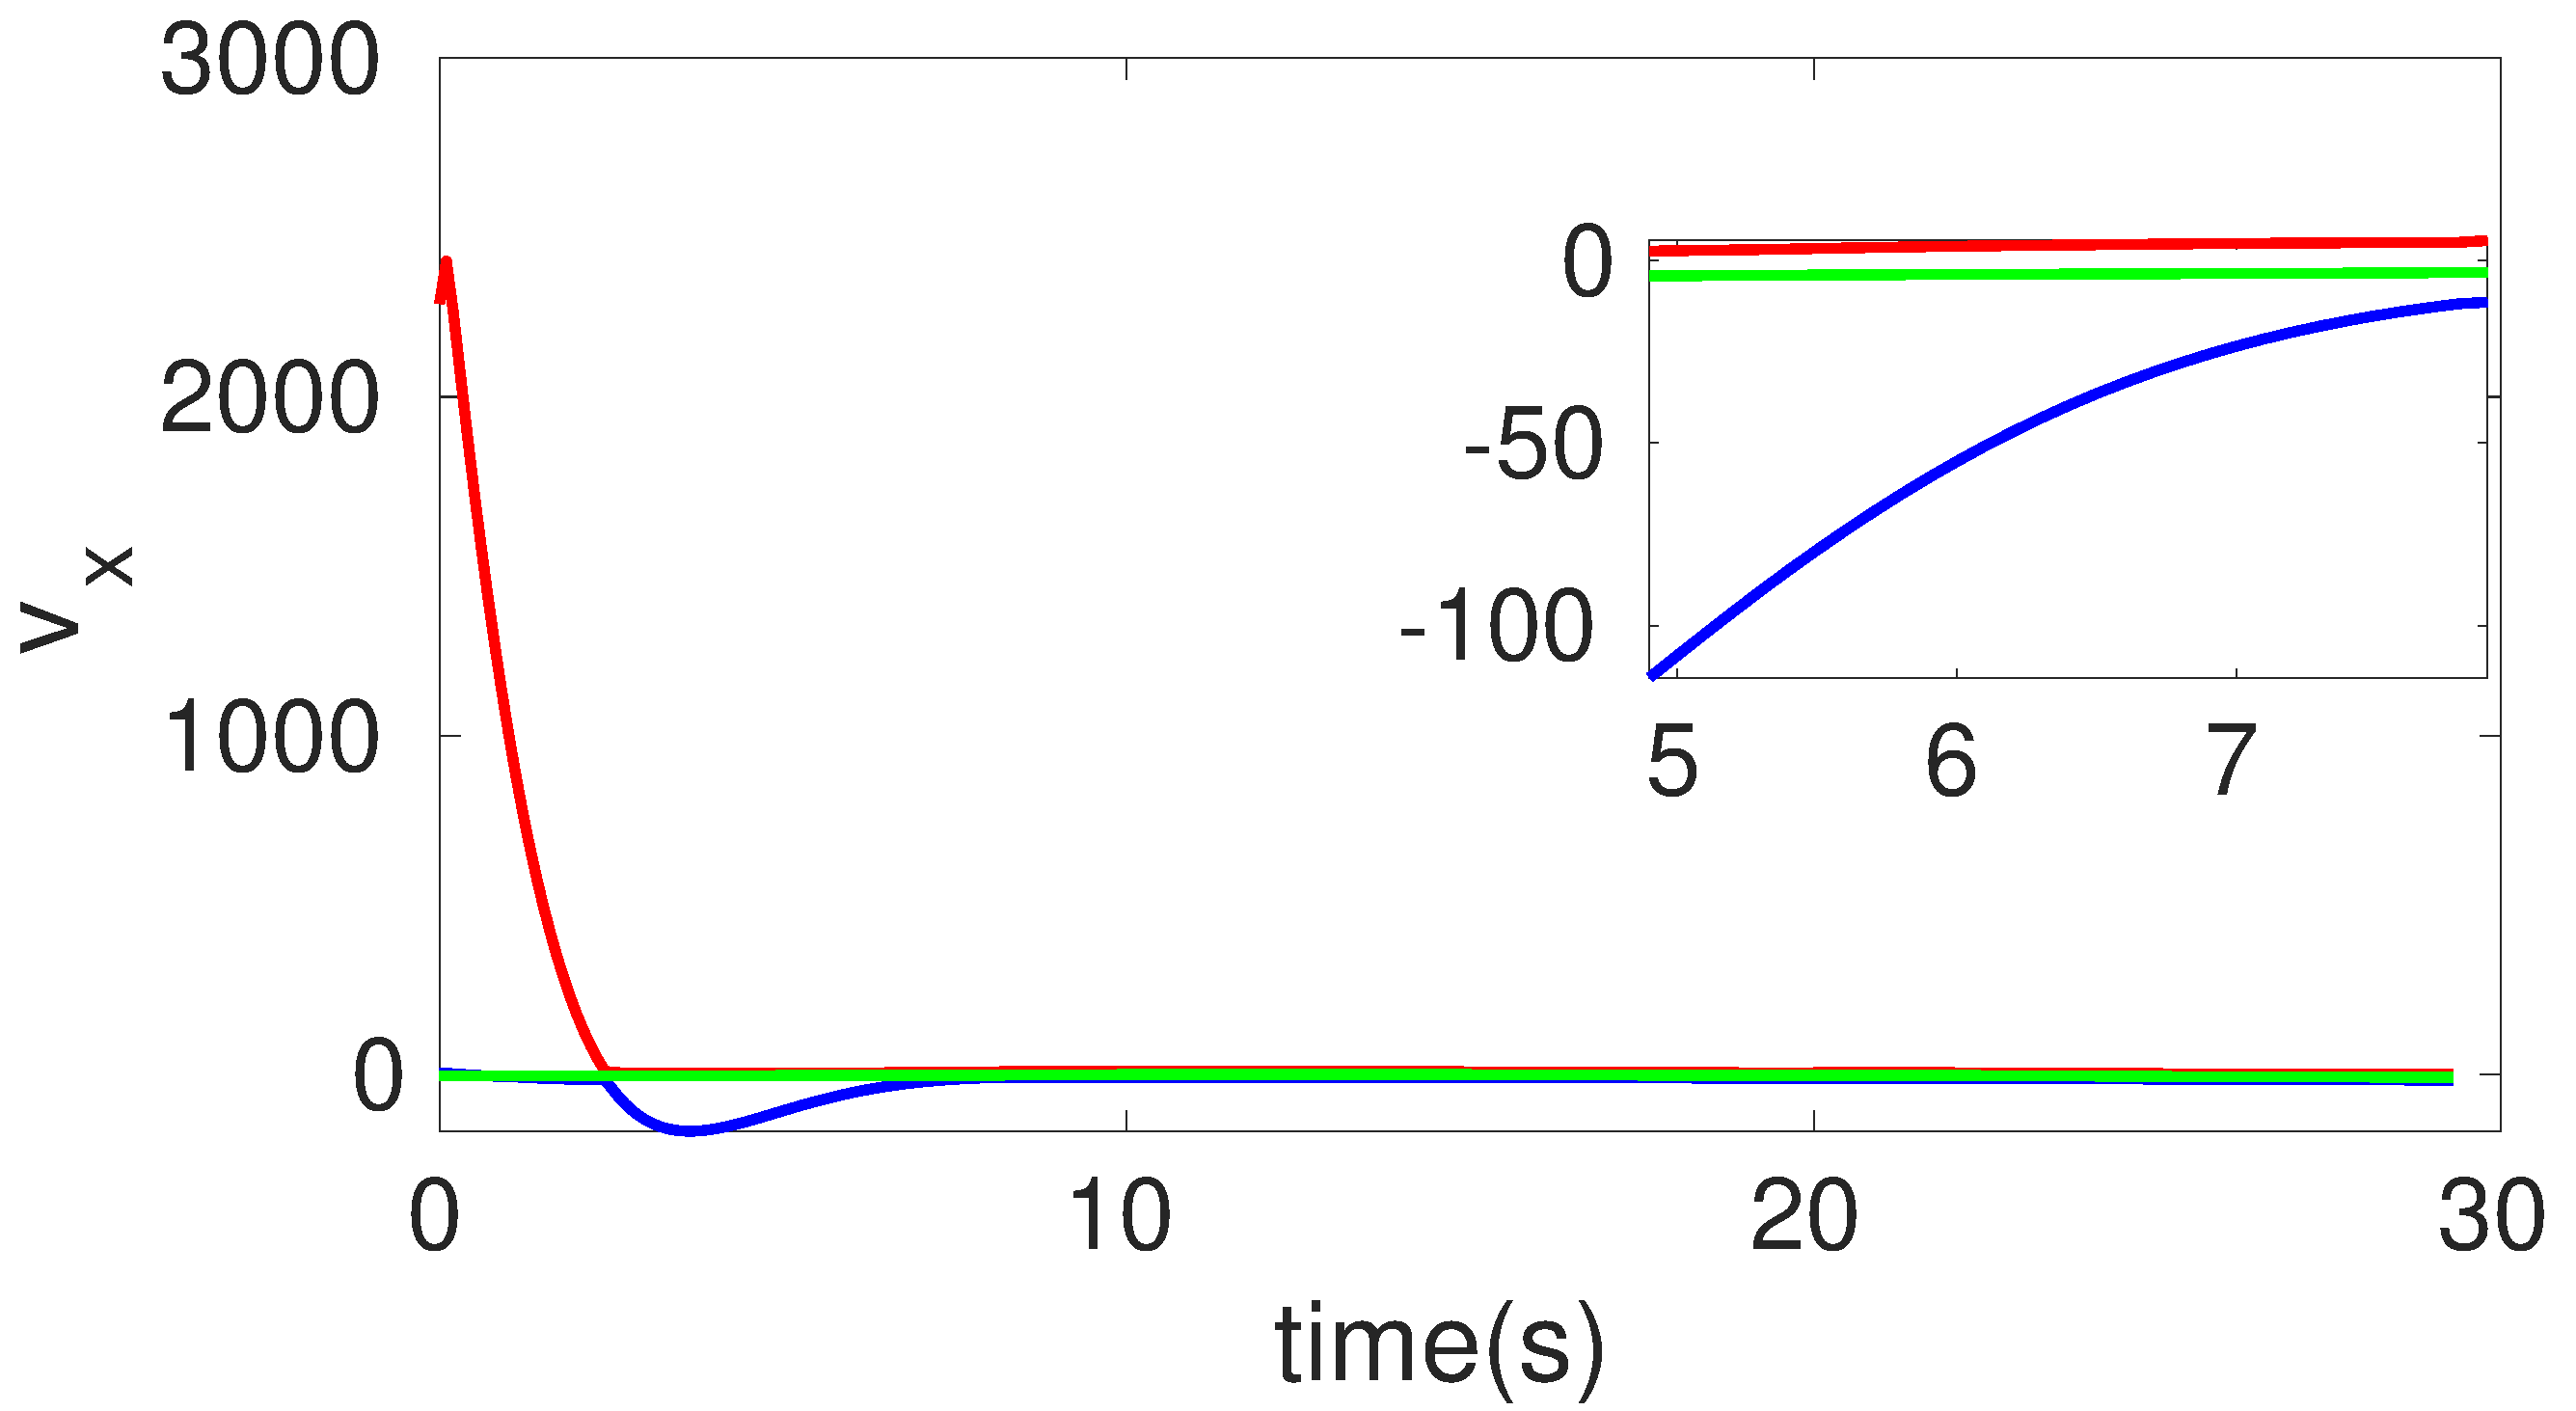
\includegraphics[width=\linewidth]{figures/Prad/s3pmpradv_x}
\end{subfigure}
\begin{subfigure}{.5\linewidth}
\centering
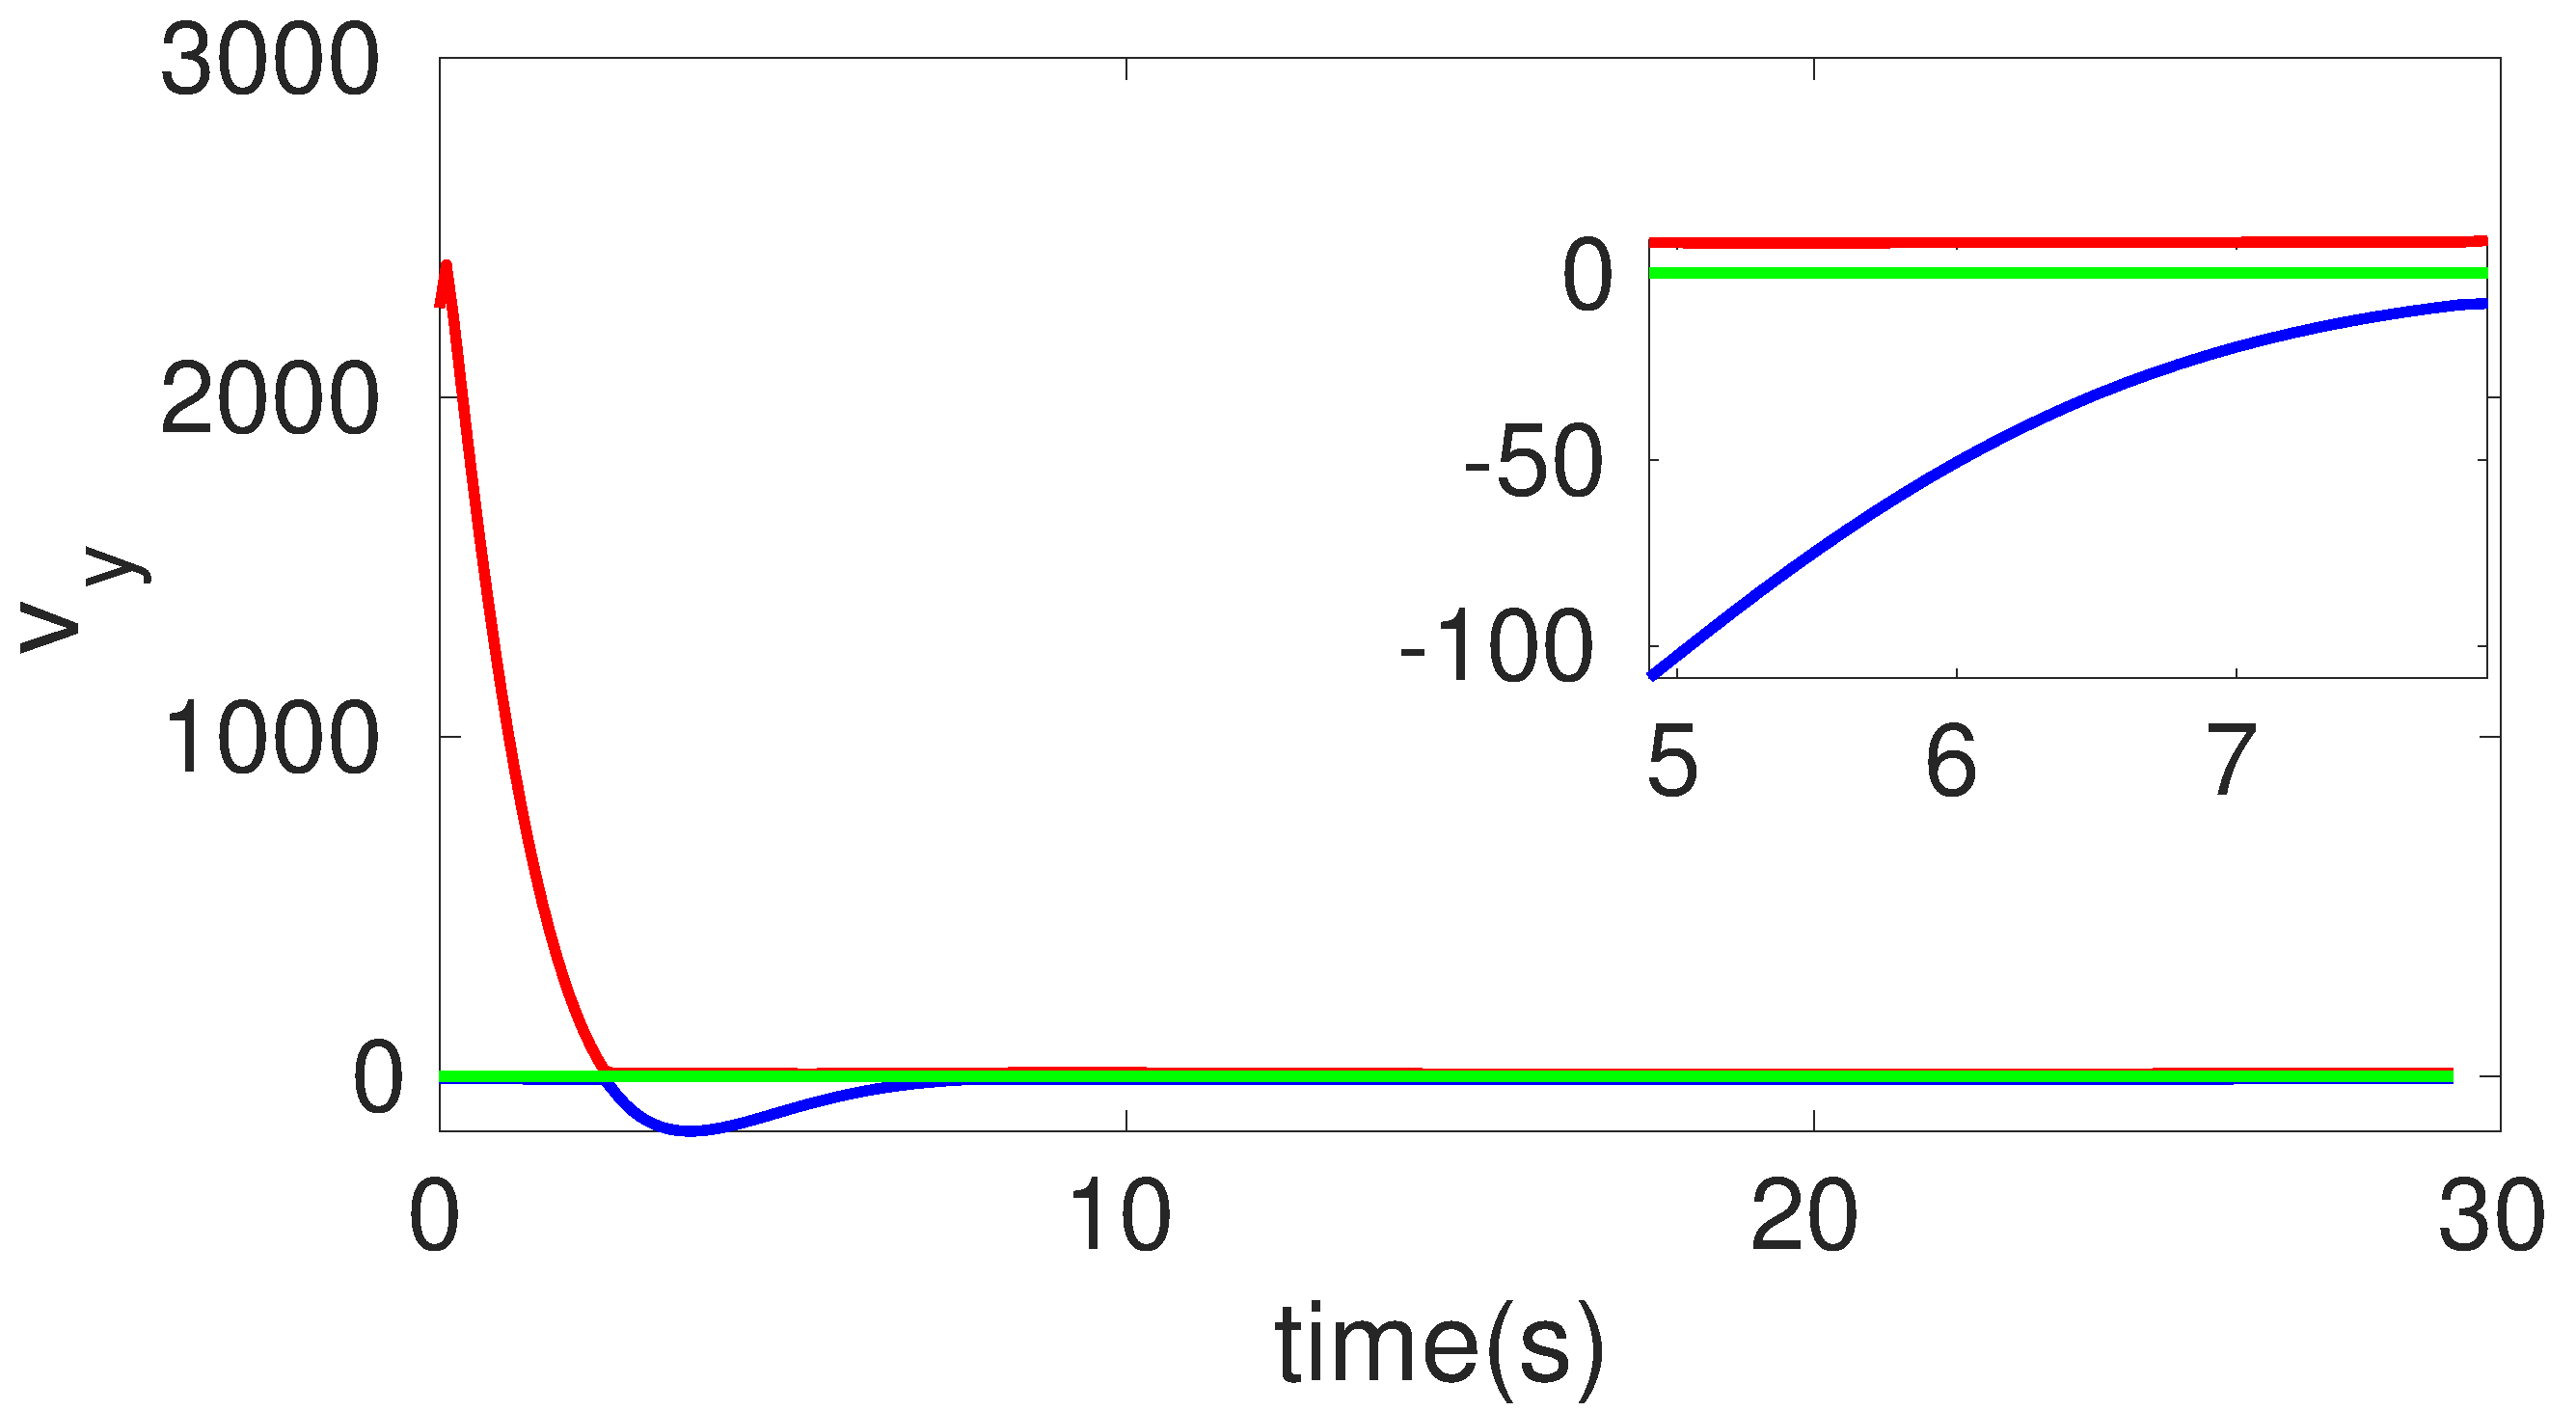
\includegraphics[width=\linewidth]{figures/Prad/s3pmpradv_y}
\end{subfigure}
\begin{subfigure}{.5\linewidth}
\centering
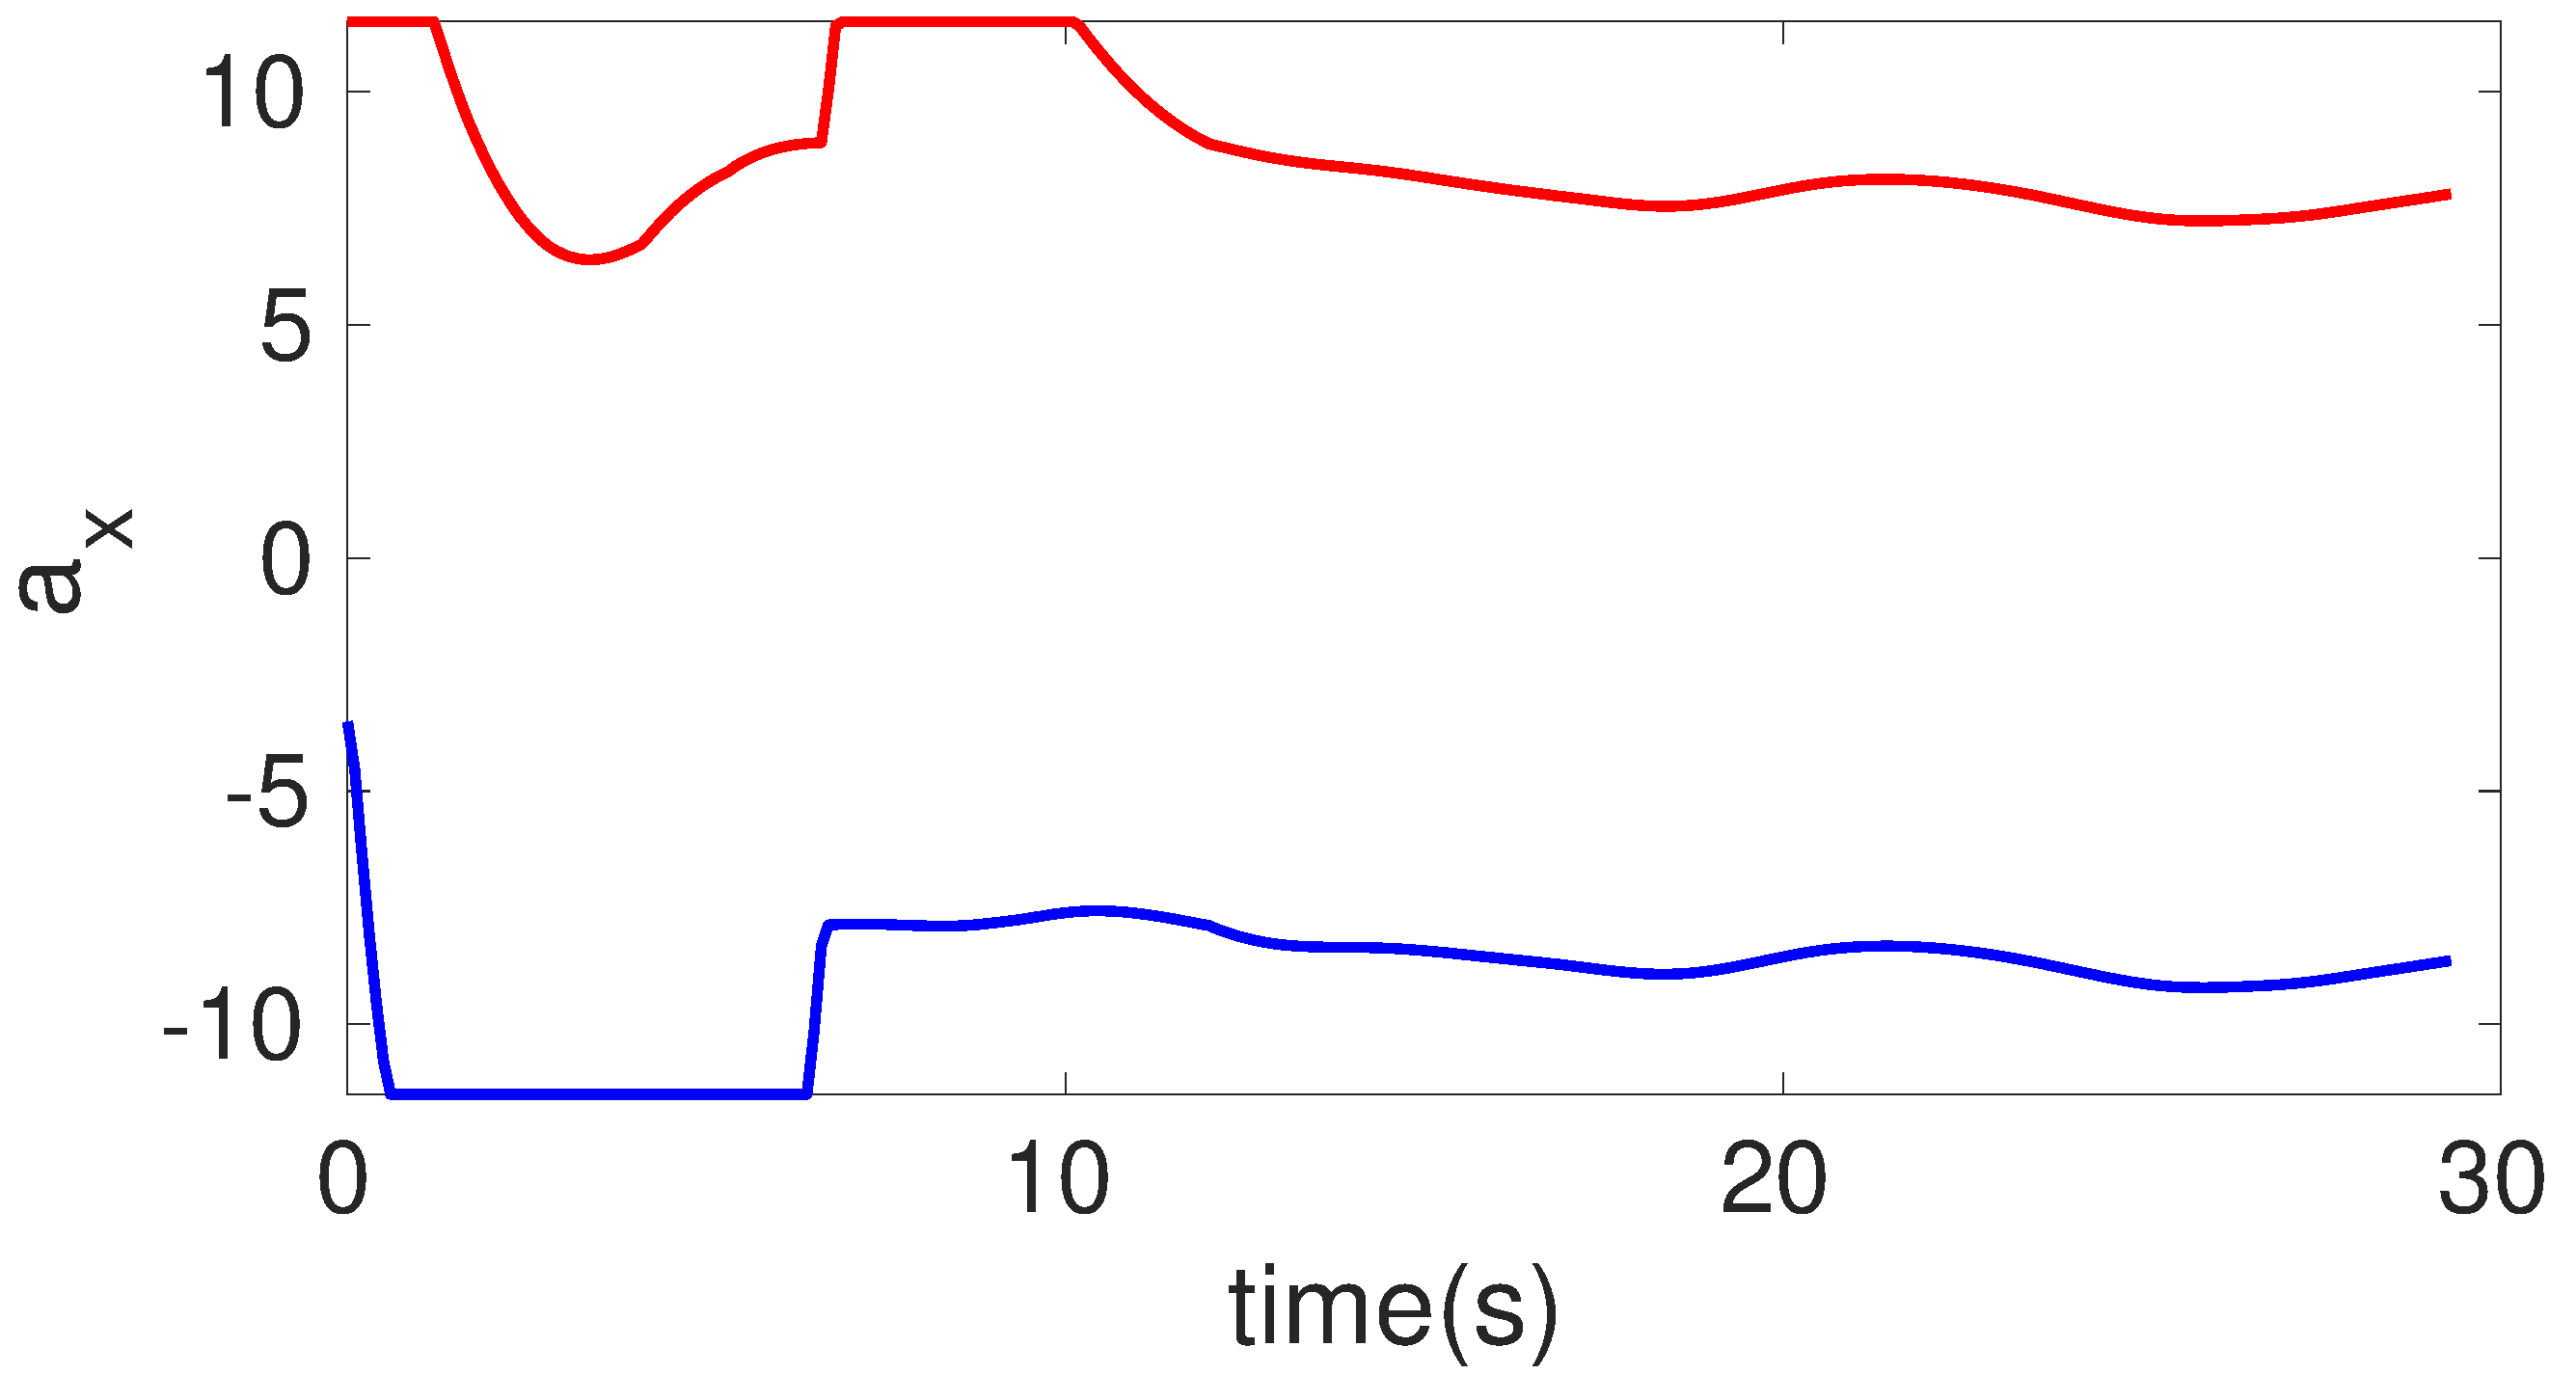
\includegraphics[width=\linewidth]{figures/Prad/s3pmprada_x}
\end{subfigure}
\begin{subfigure}{.5\linewidth}
\centering
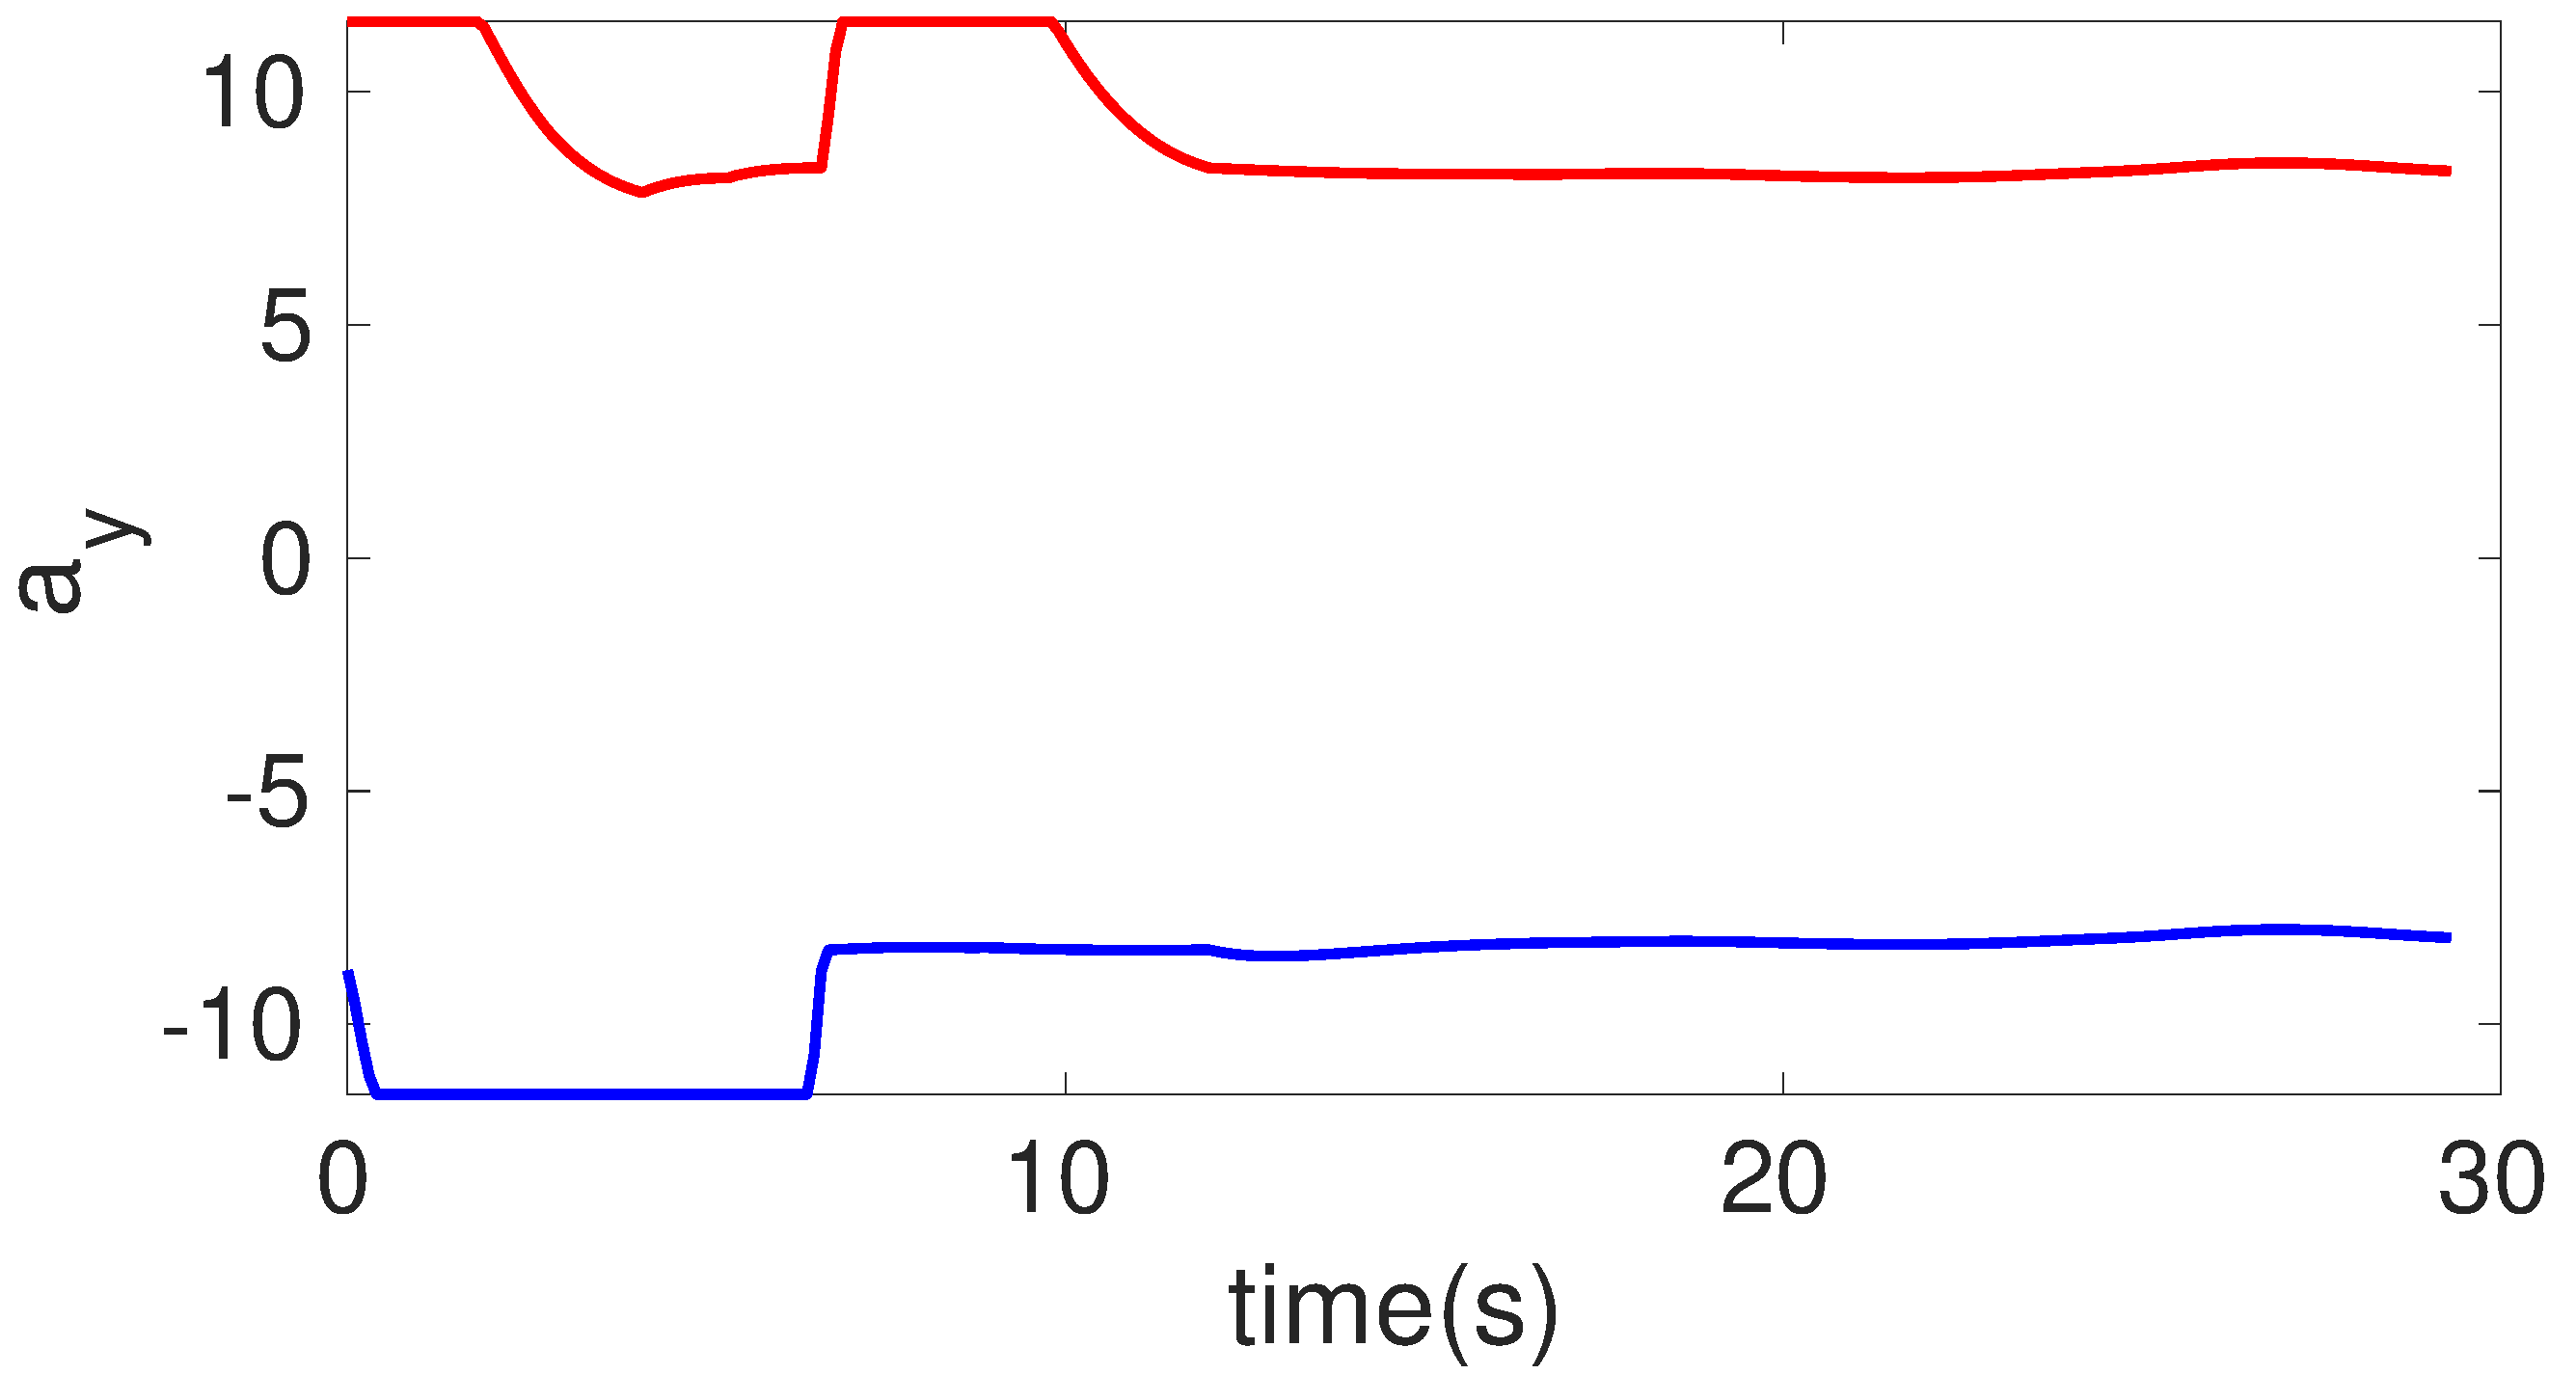
\includegraphics[width=\linewidth]{figures/Prad/s3pmprada_y}
\end{subfigure}
\caption{Estimation using the P-radius minimizer and the point-mass model}
\end{figure}


\clearpage
\subsection{Interval Observer using H-$\infty$}\label{eresult:hinf}
\FloatBarrier
\begin{figure}[!h]
\hspace*{\fill} 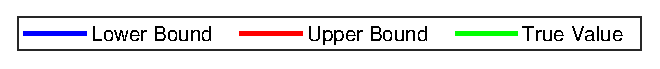
\includegraphics[scale=0.8]{figures/legend}\\\\
\begin{subfigure}{.5\linewidth}
\centering
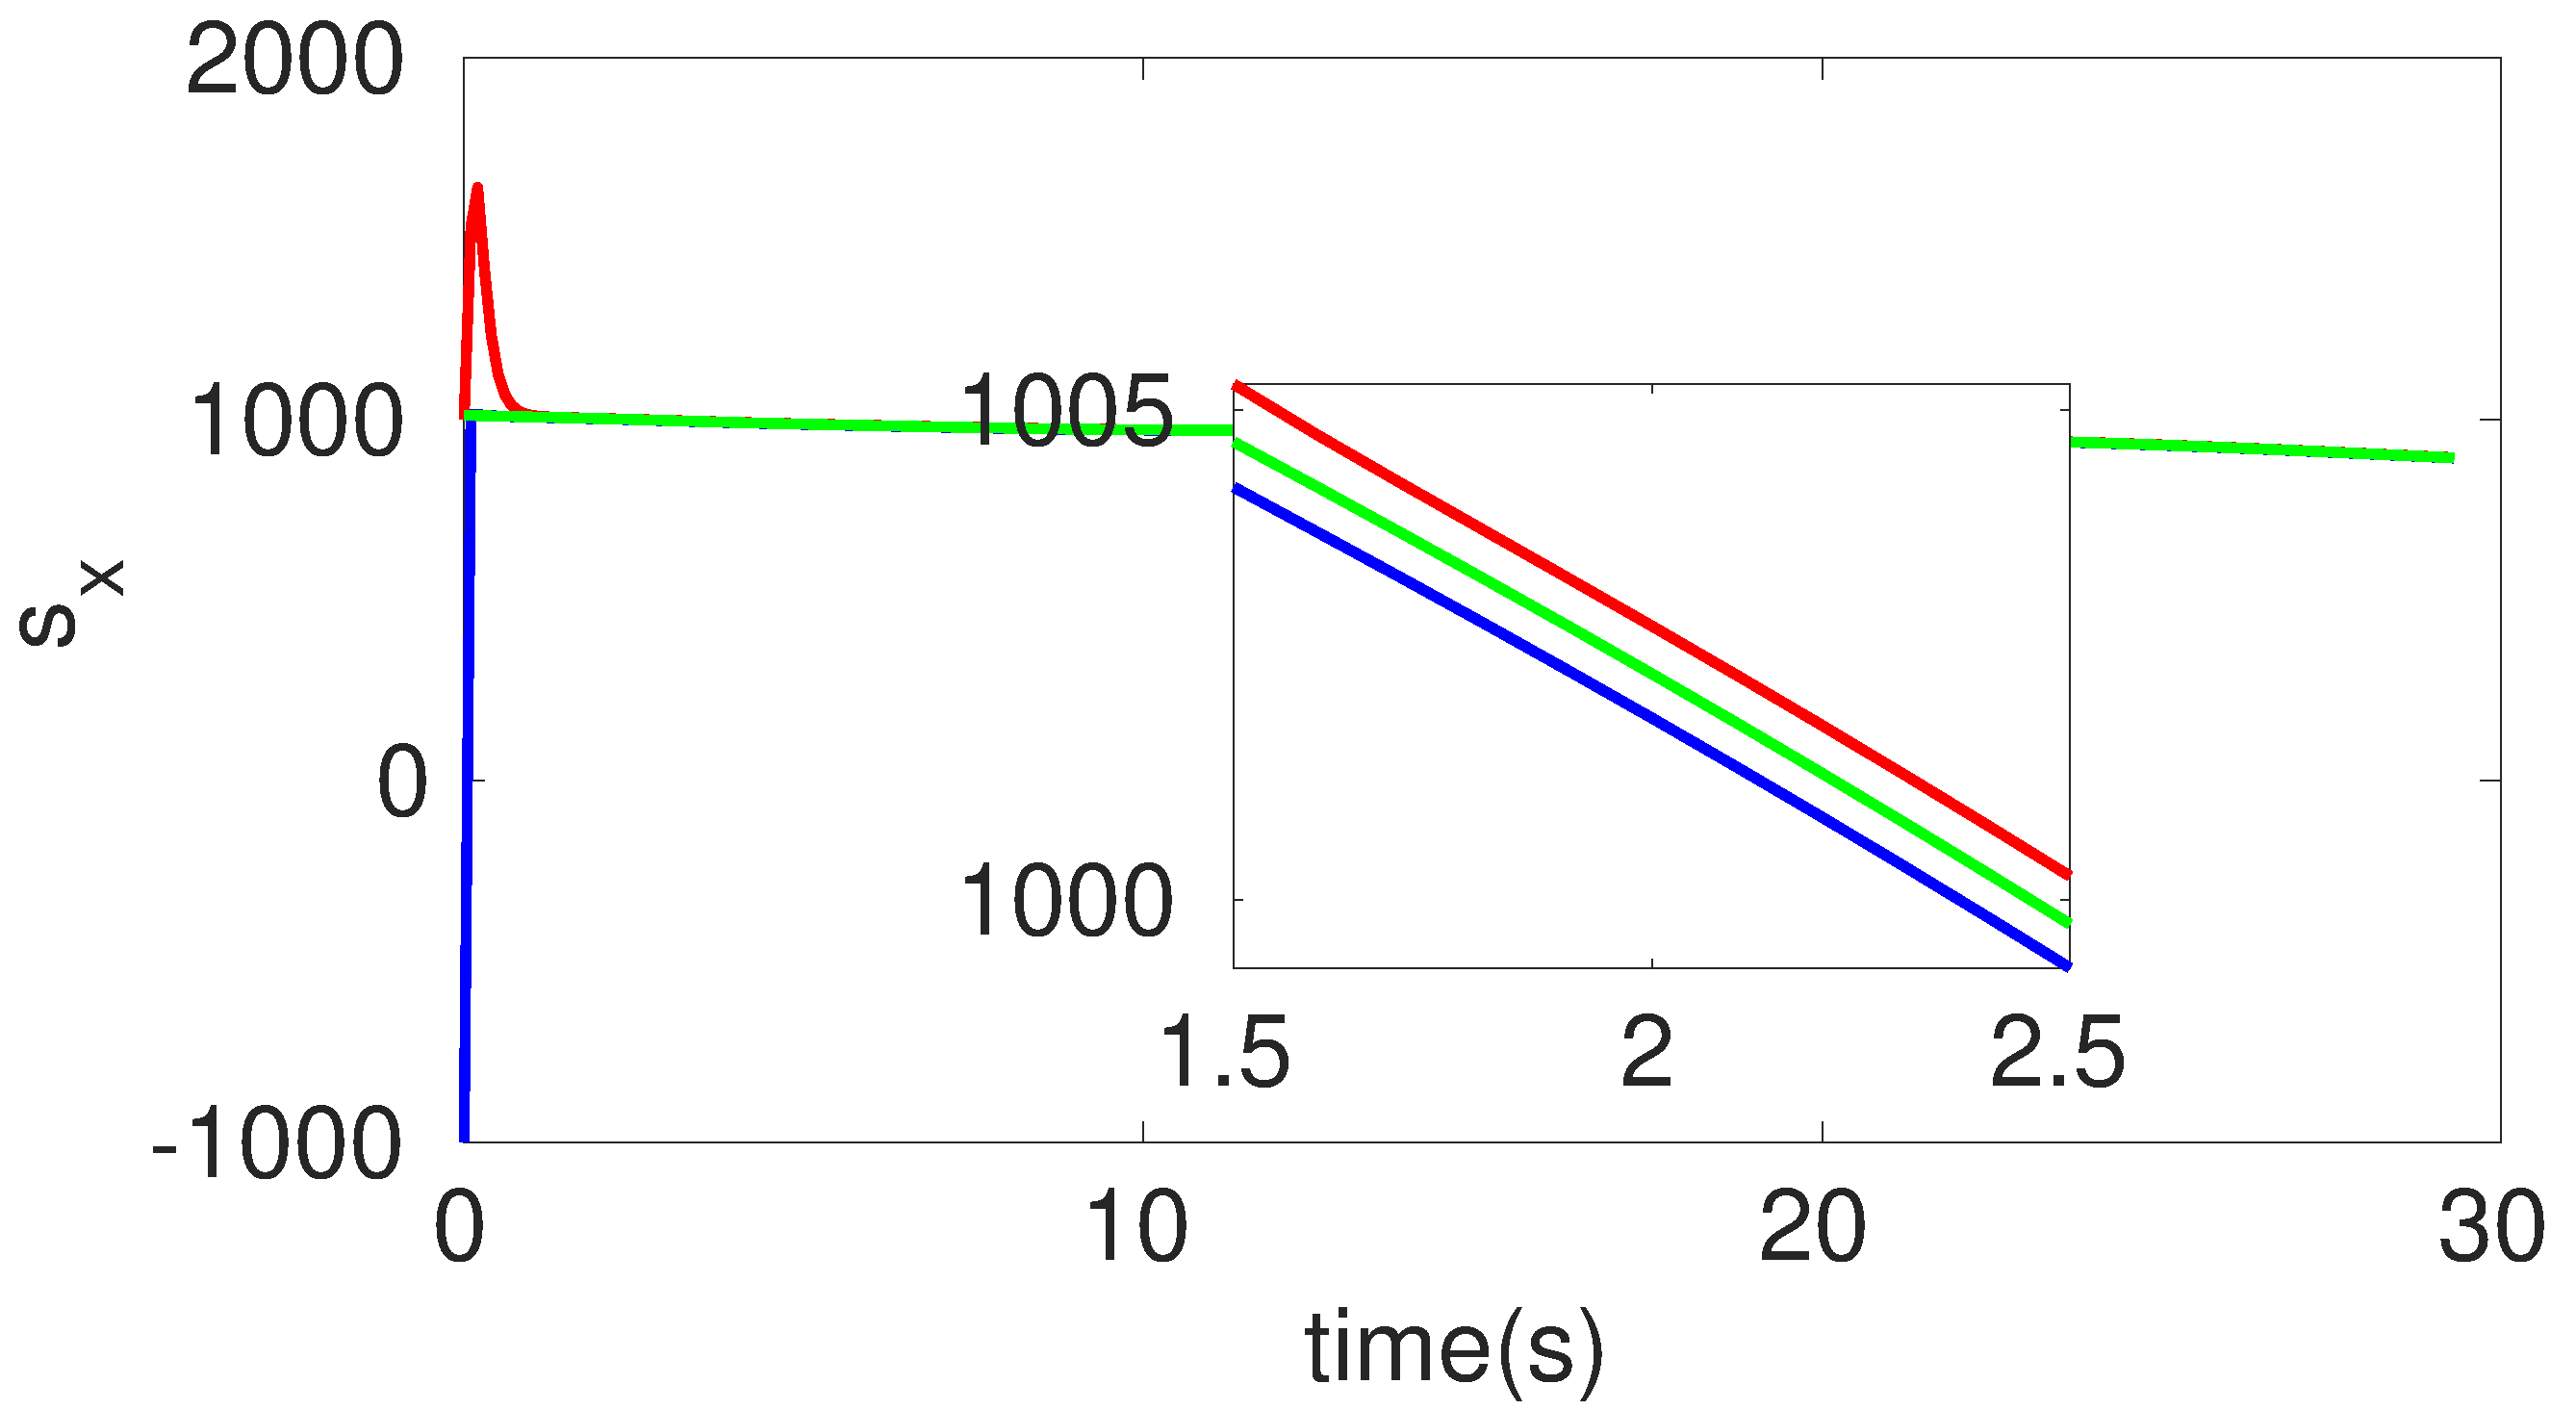
\includegraphics[width=\linewidth]{figures/HInf/s3cvHInfs_x}
\end{subfigure}
\begin{subfigure}{.5\linewidth}
\centering
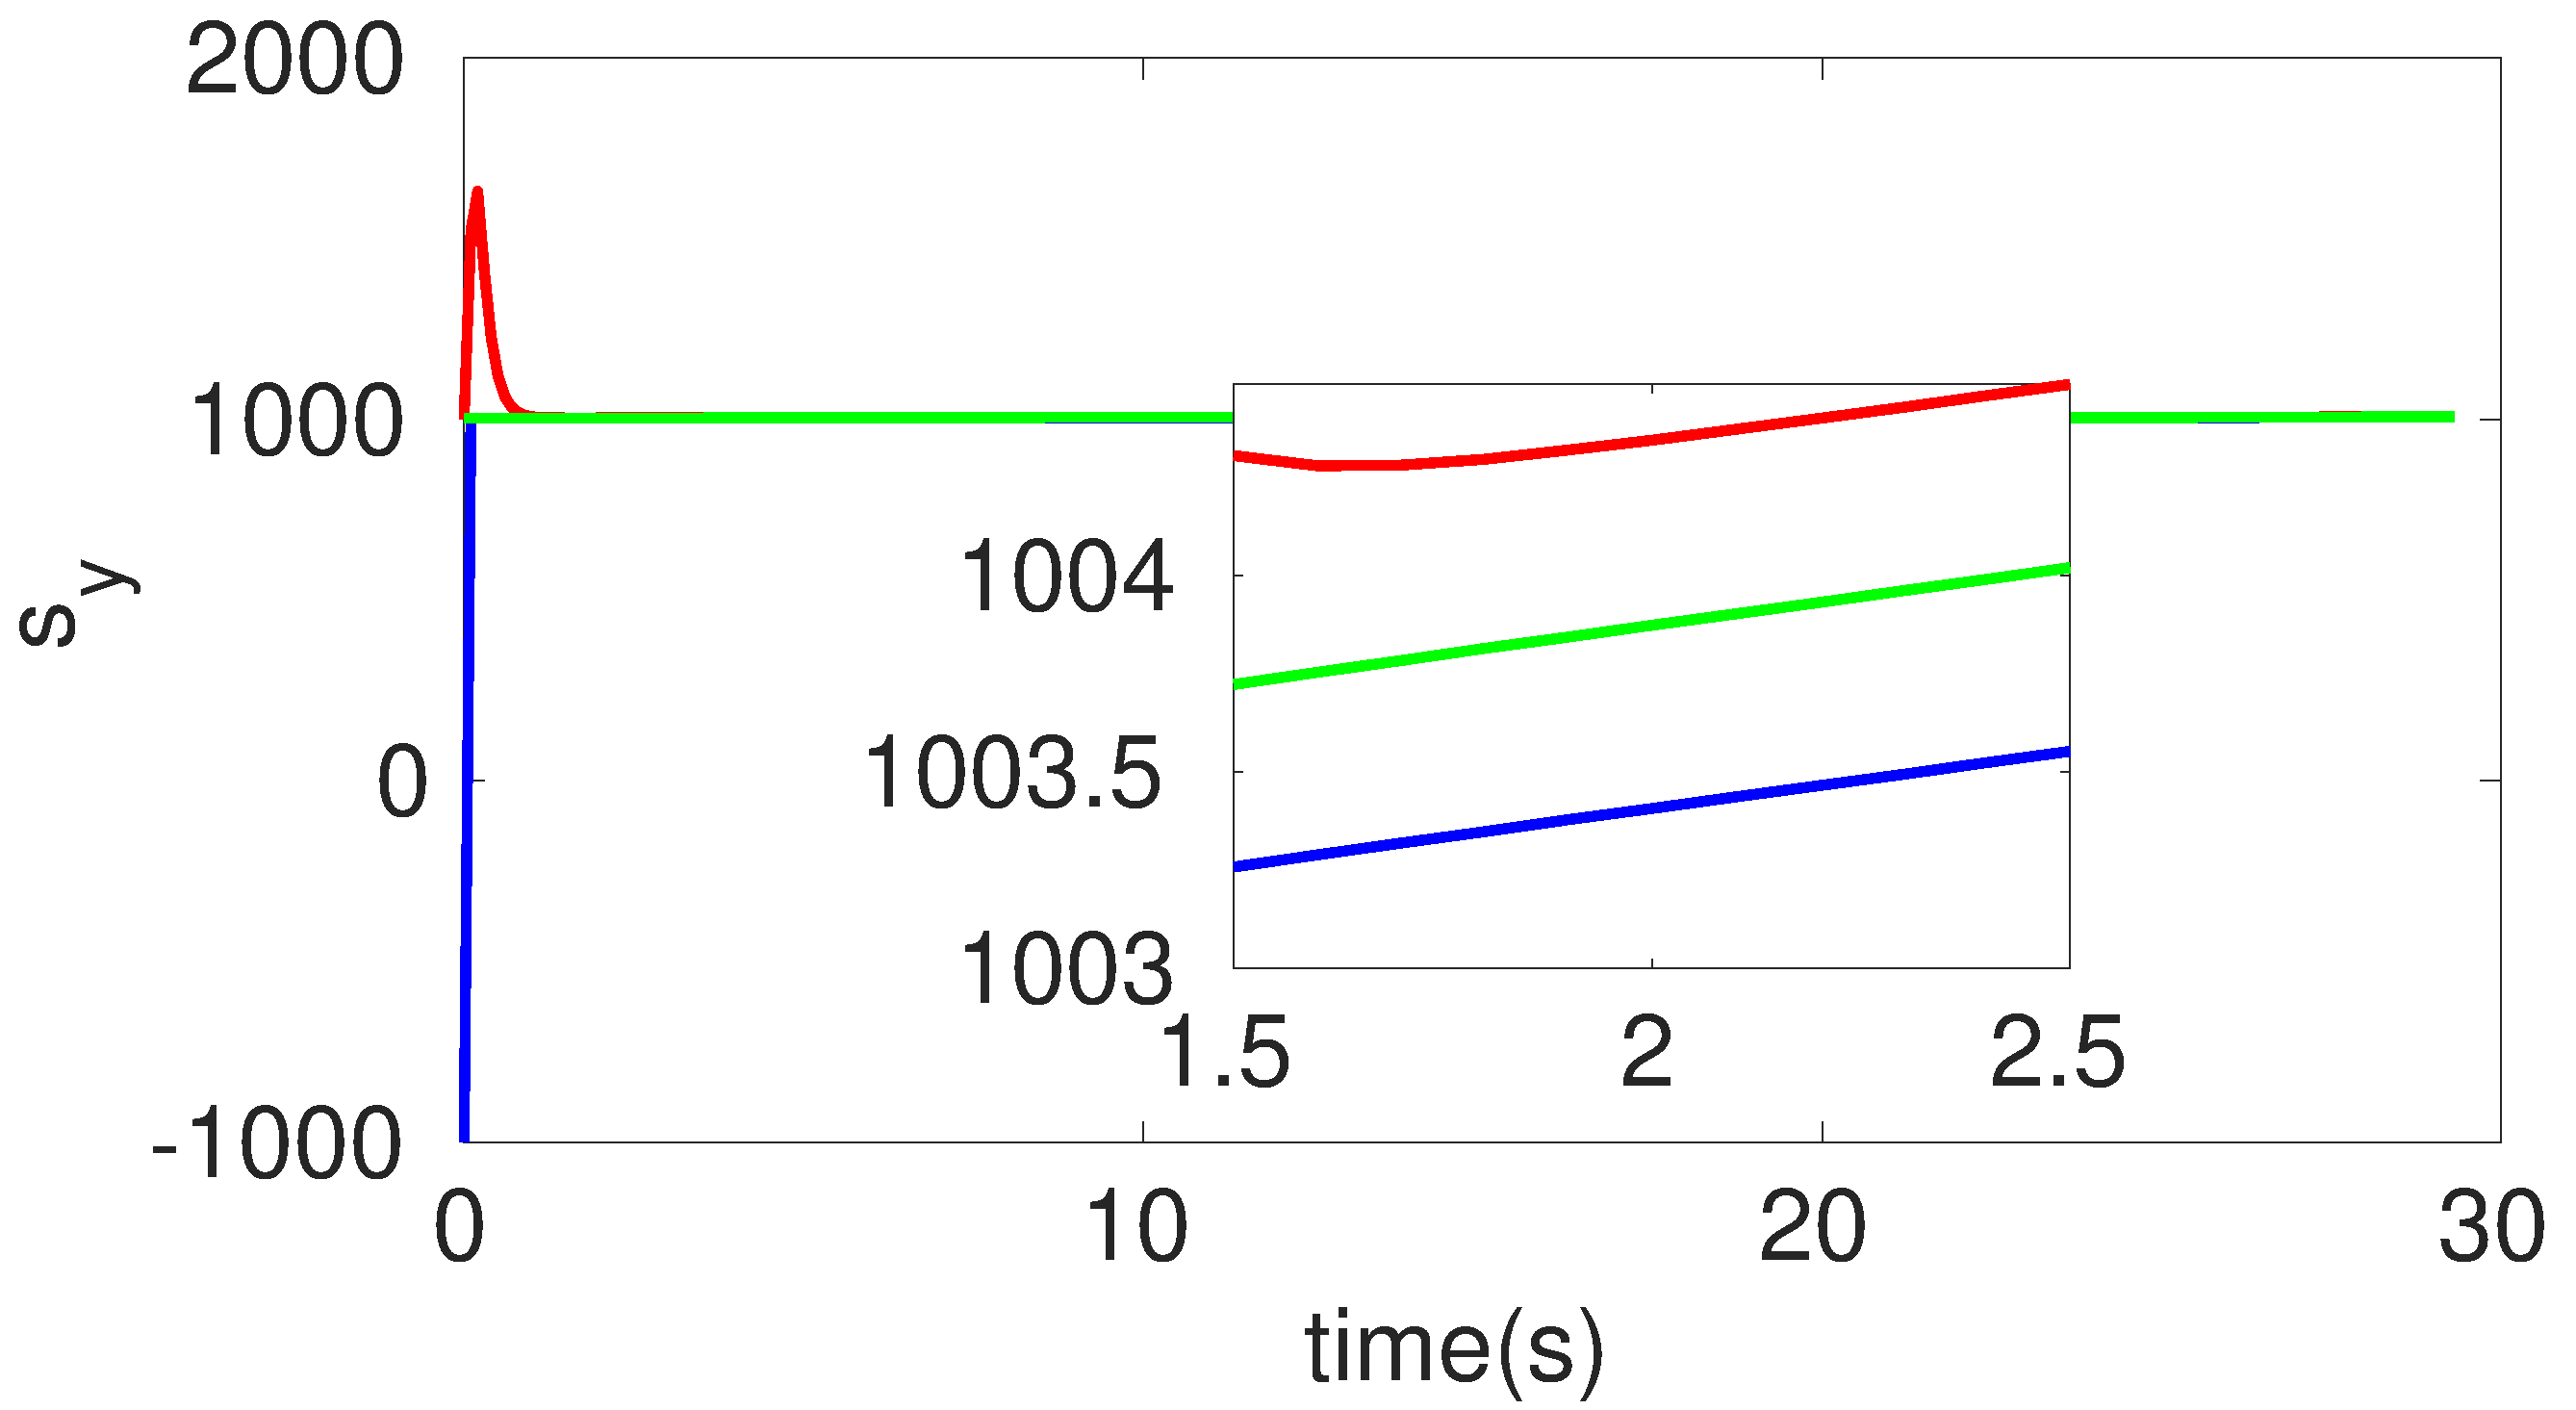
\includegraphics[width=\linewidth]{figures/HInf/s3cvHInfs_y}
\end{subfigure}
\begin{subfigure}{.5\linewidth}
\centering
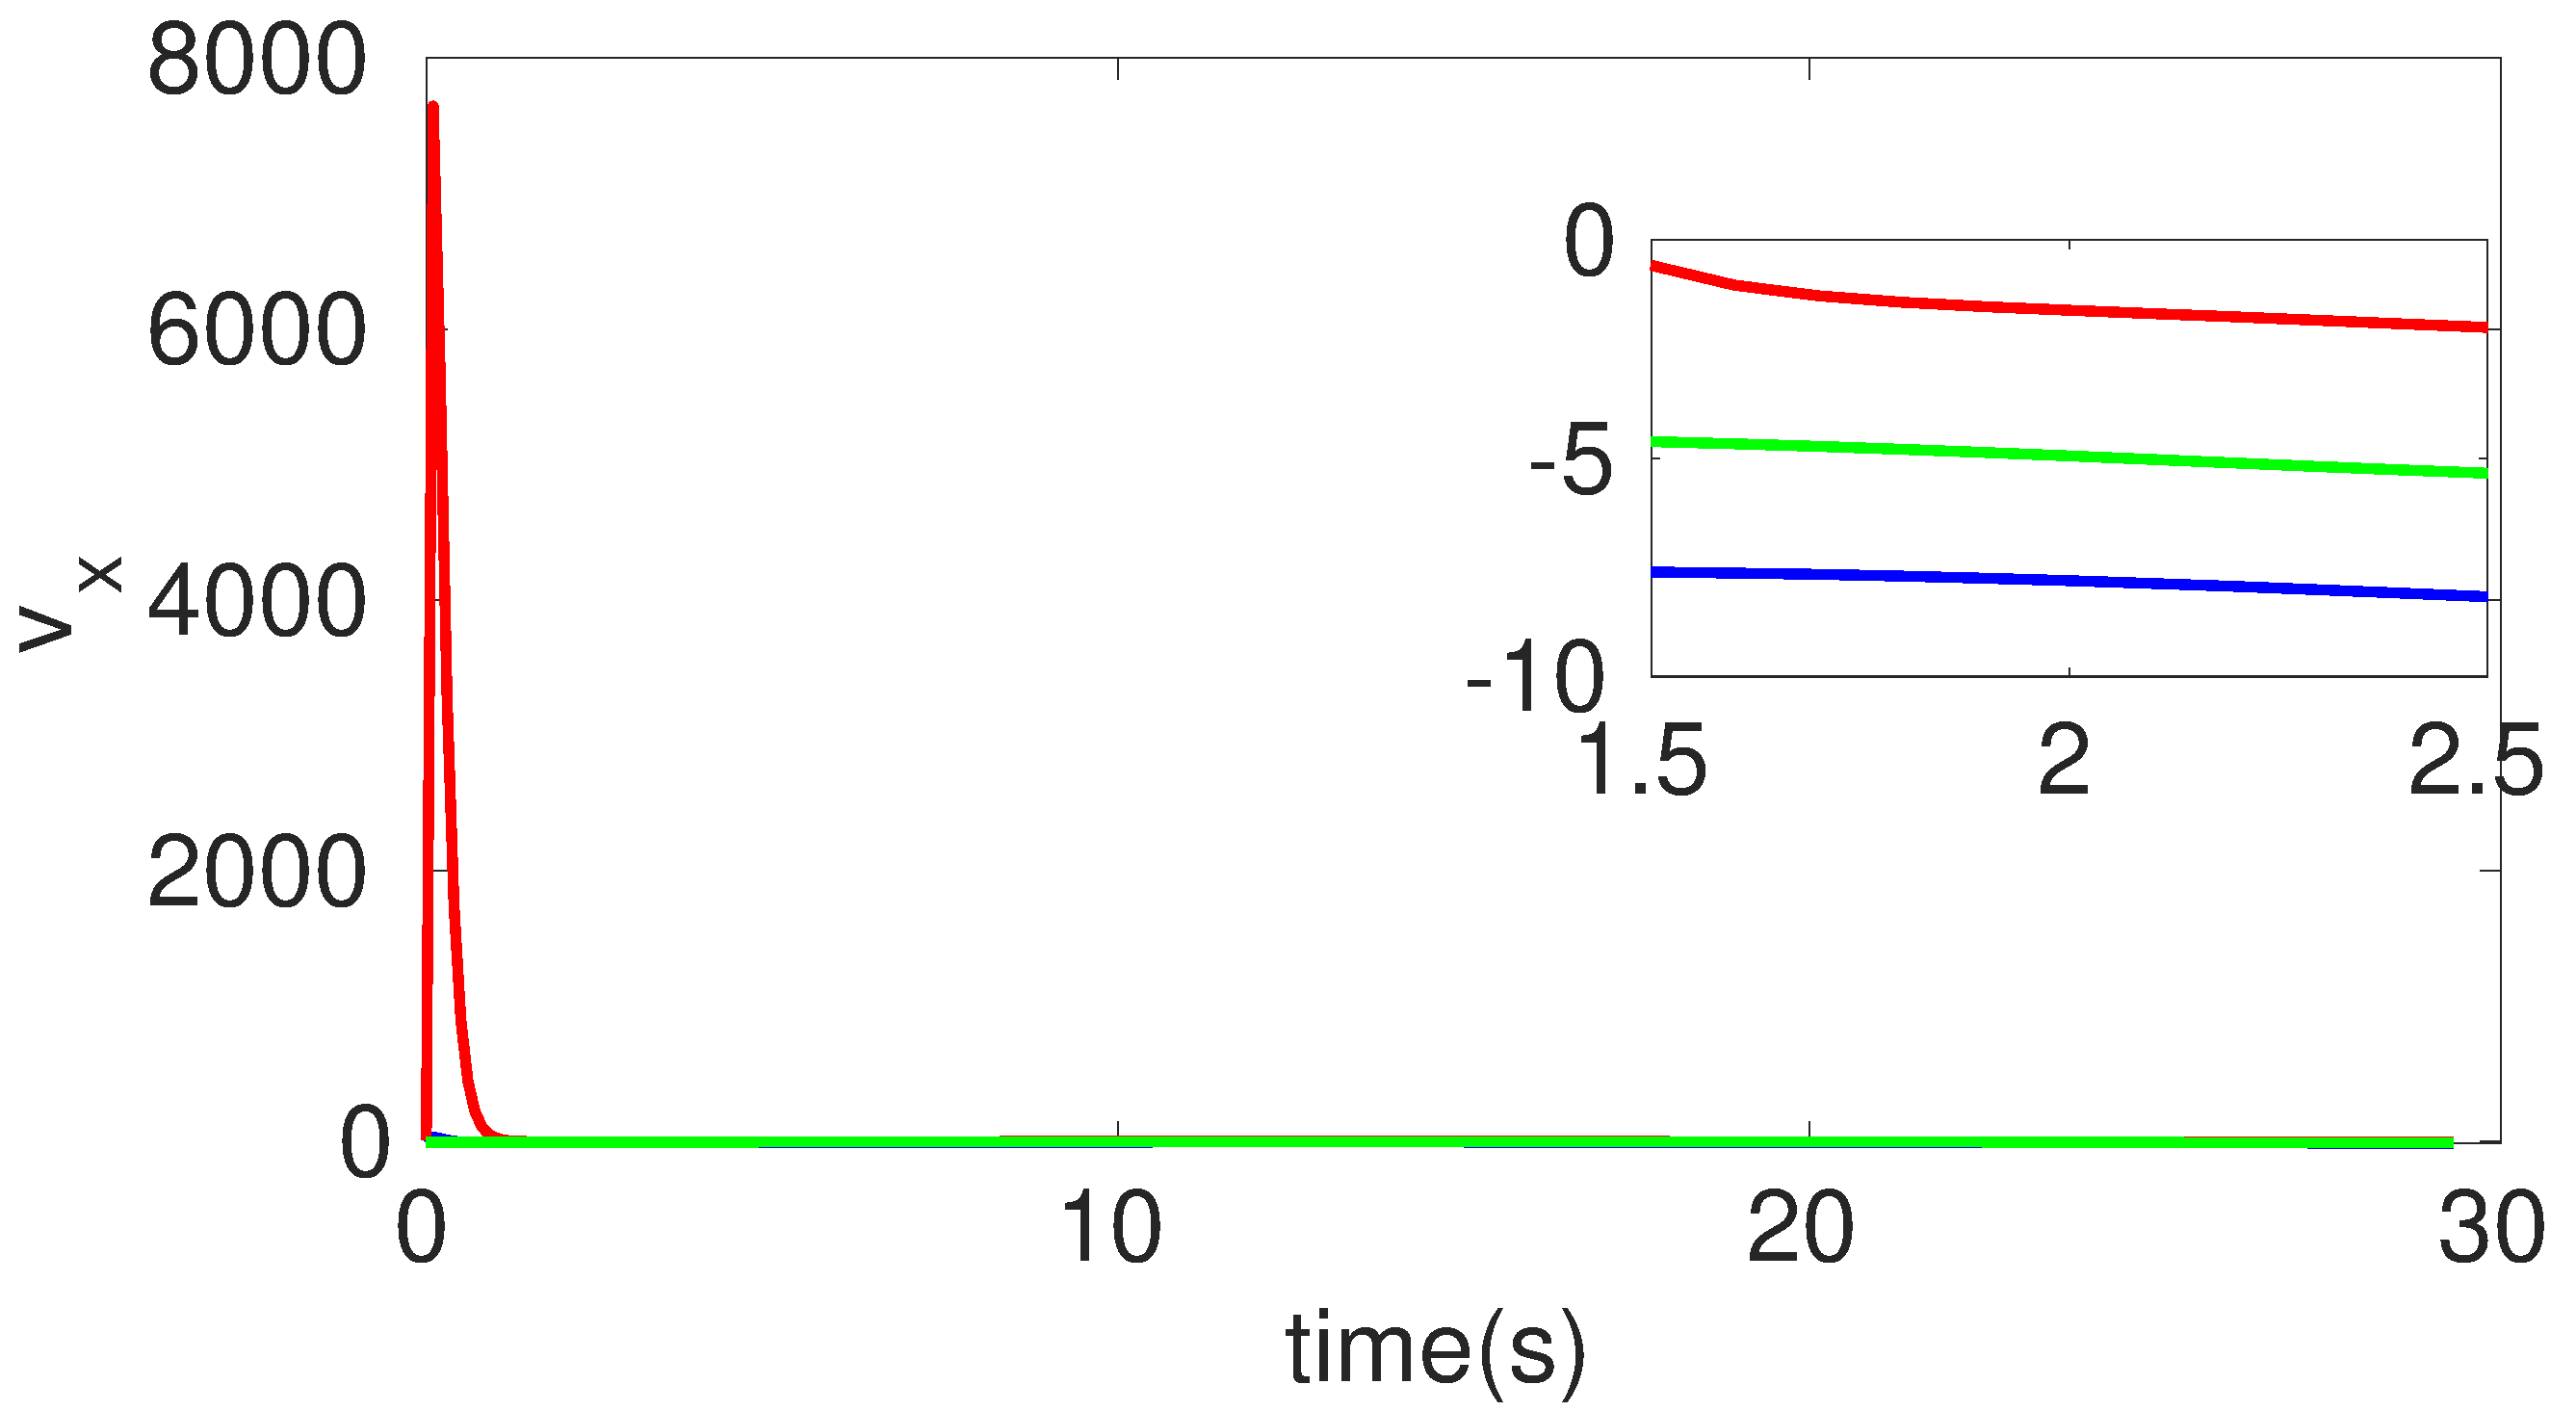
\includegraphics[width=\linewidth]{figures/HInf/s3cvHInfv_x}
\end{subfigure}
\begin{subfigure}{.5\linewidth}
\centering
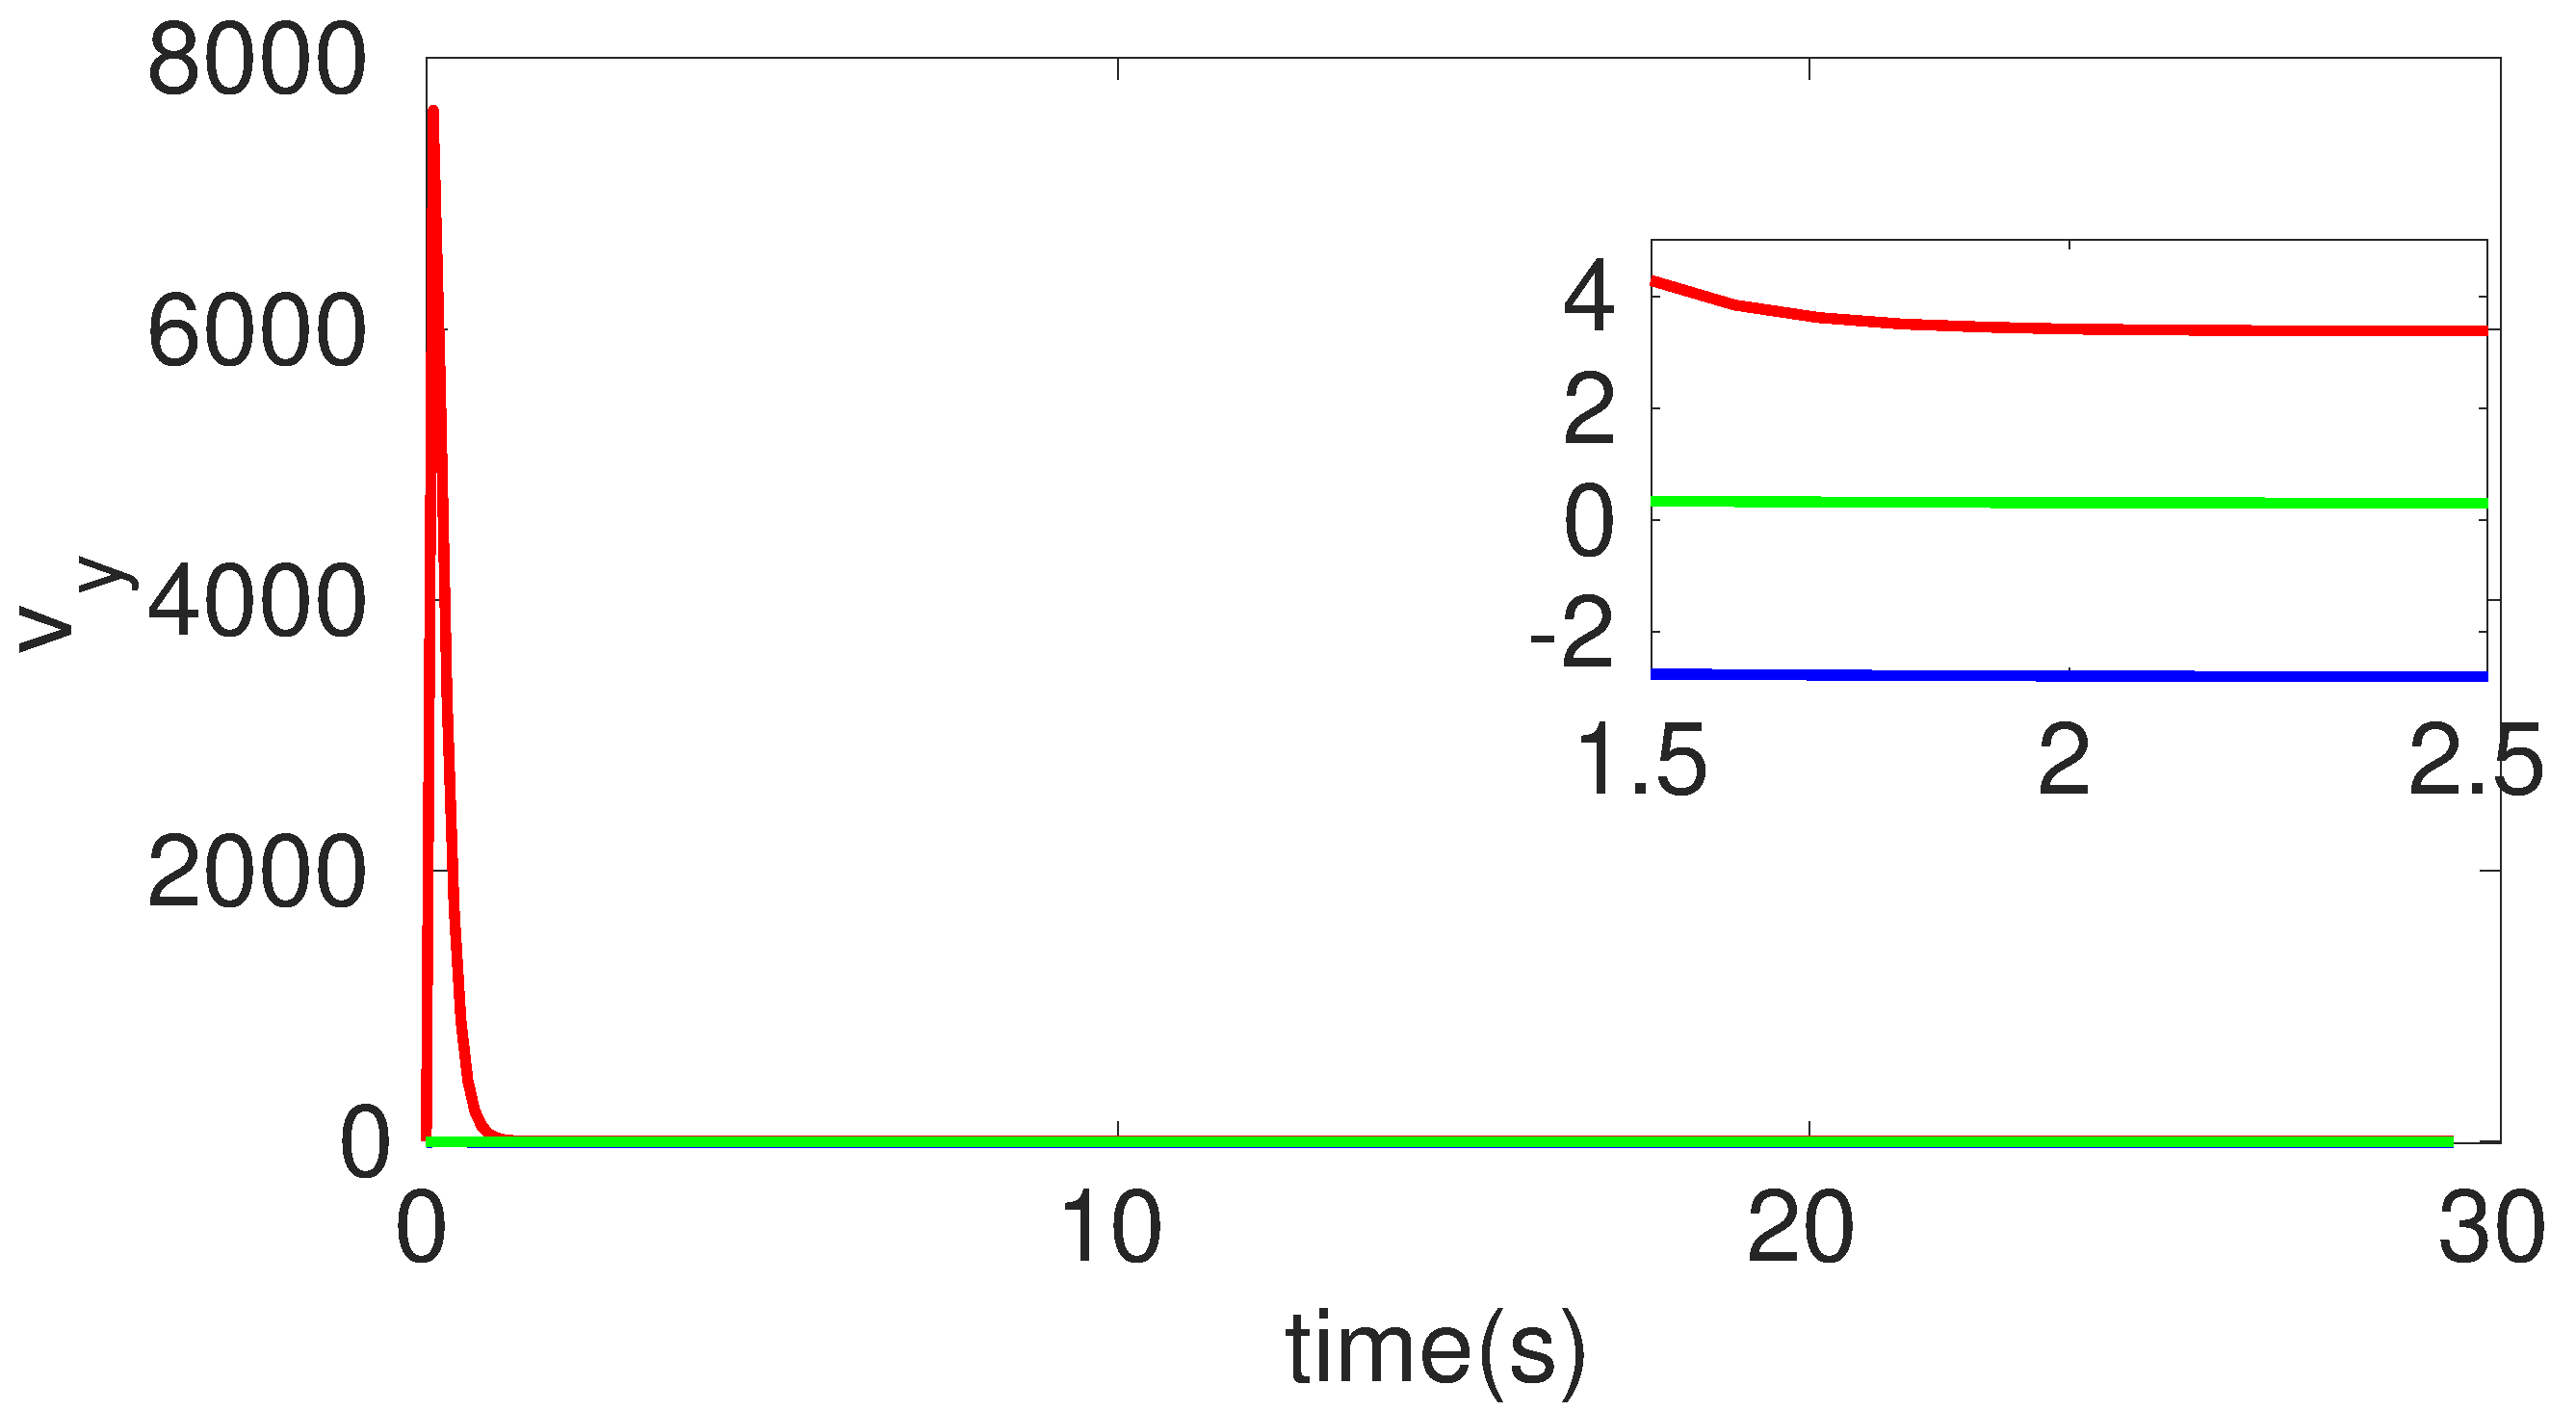
\includegraphics[width=\linewidth]{figures/HInf/s3cvHInfv_y}
\end{subfigure}
\caption{Estimation using the H-$\infty$ observer and the constant velocity model}
\end{figure}

\begin{figure}[!h]
\hspace*{\fill} 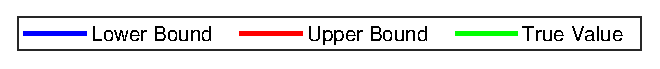
\includegraphics[scale=0.8]{figures/legend}\\\\
\begin{subfigure}{.5\linewidth}
\centering
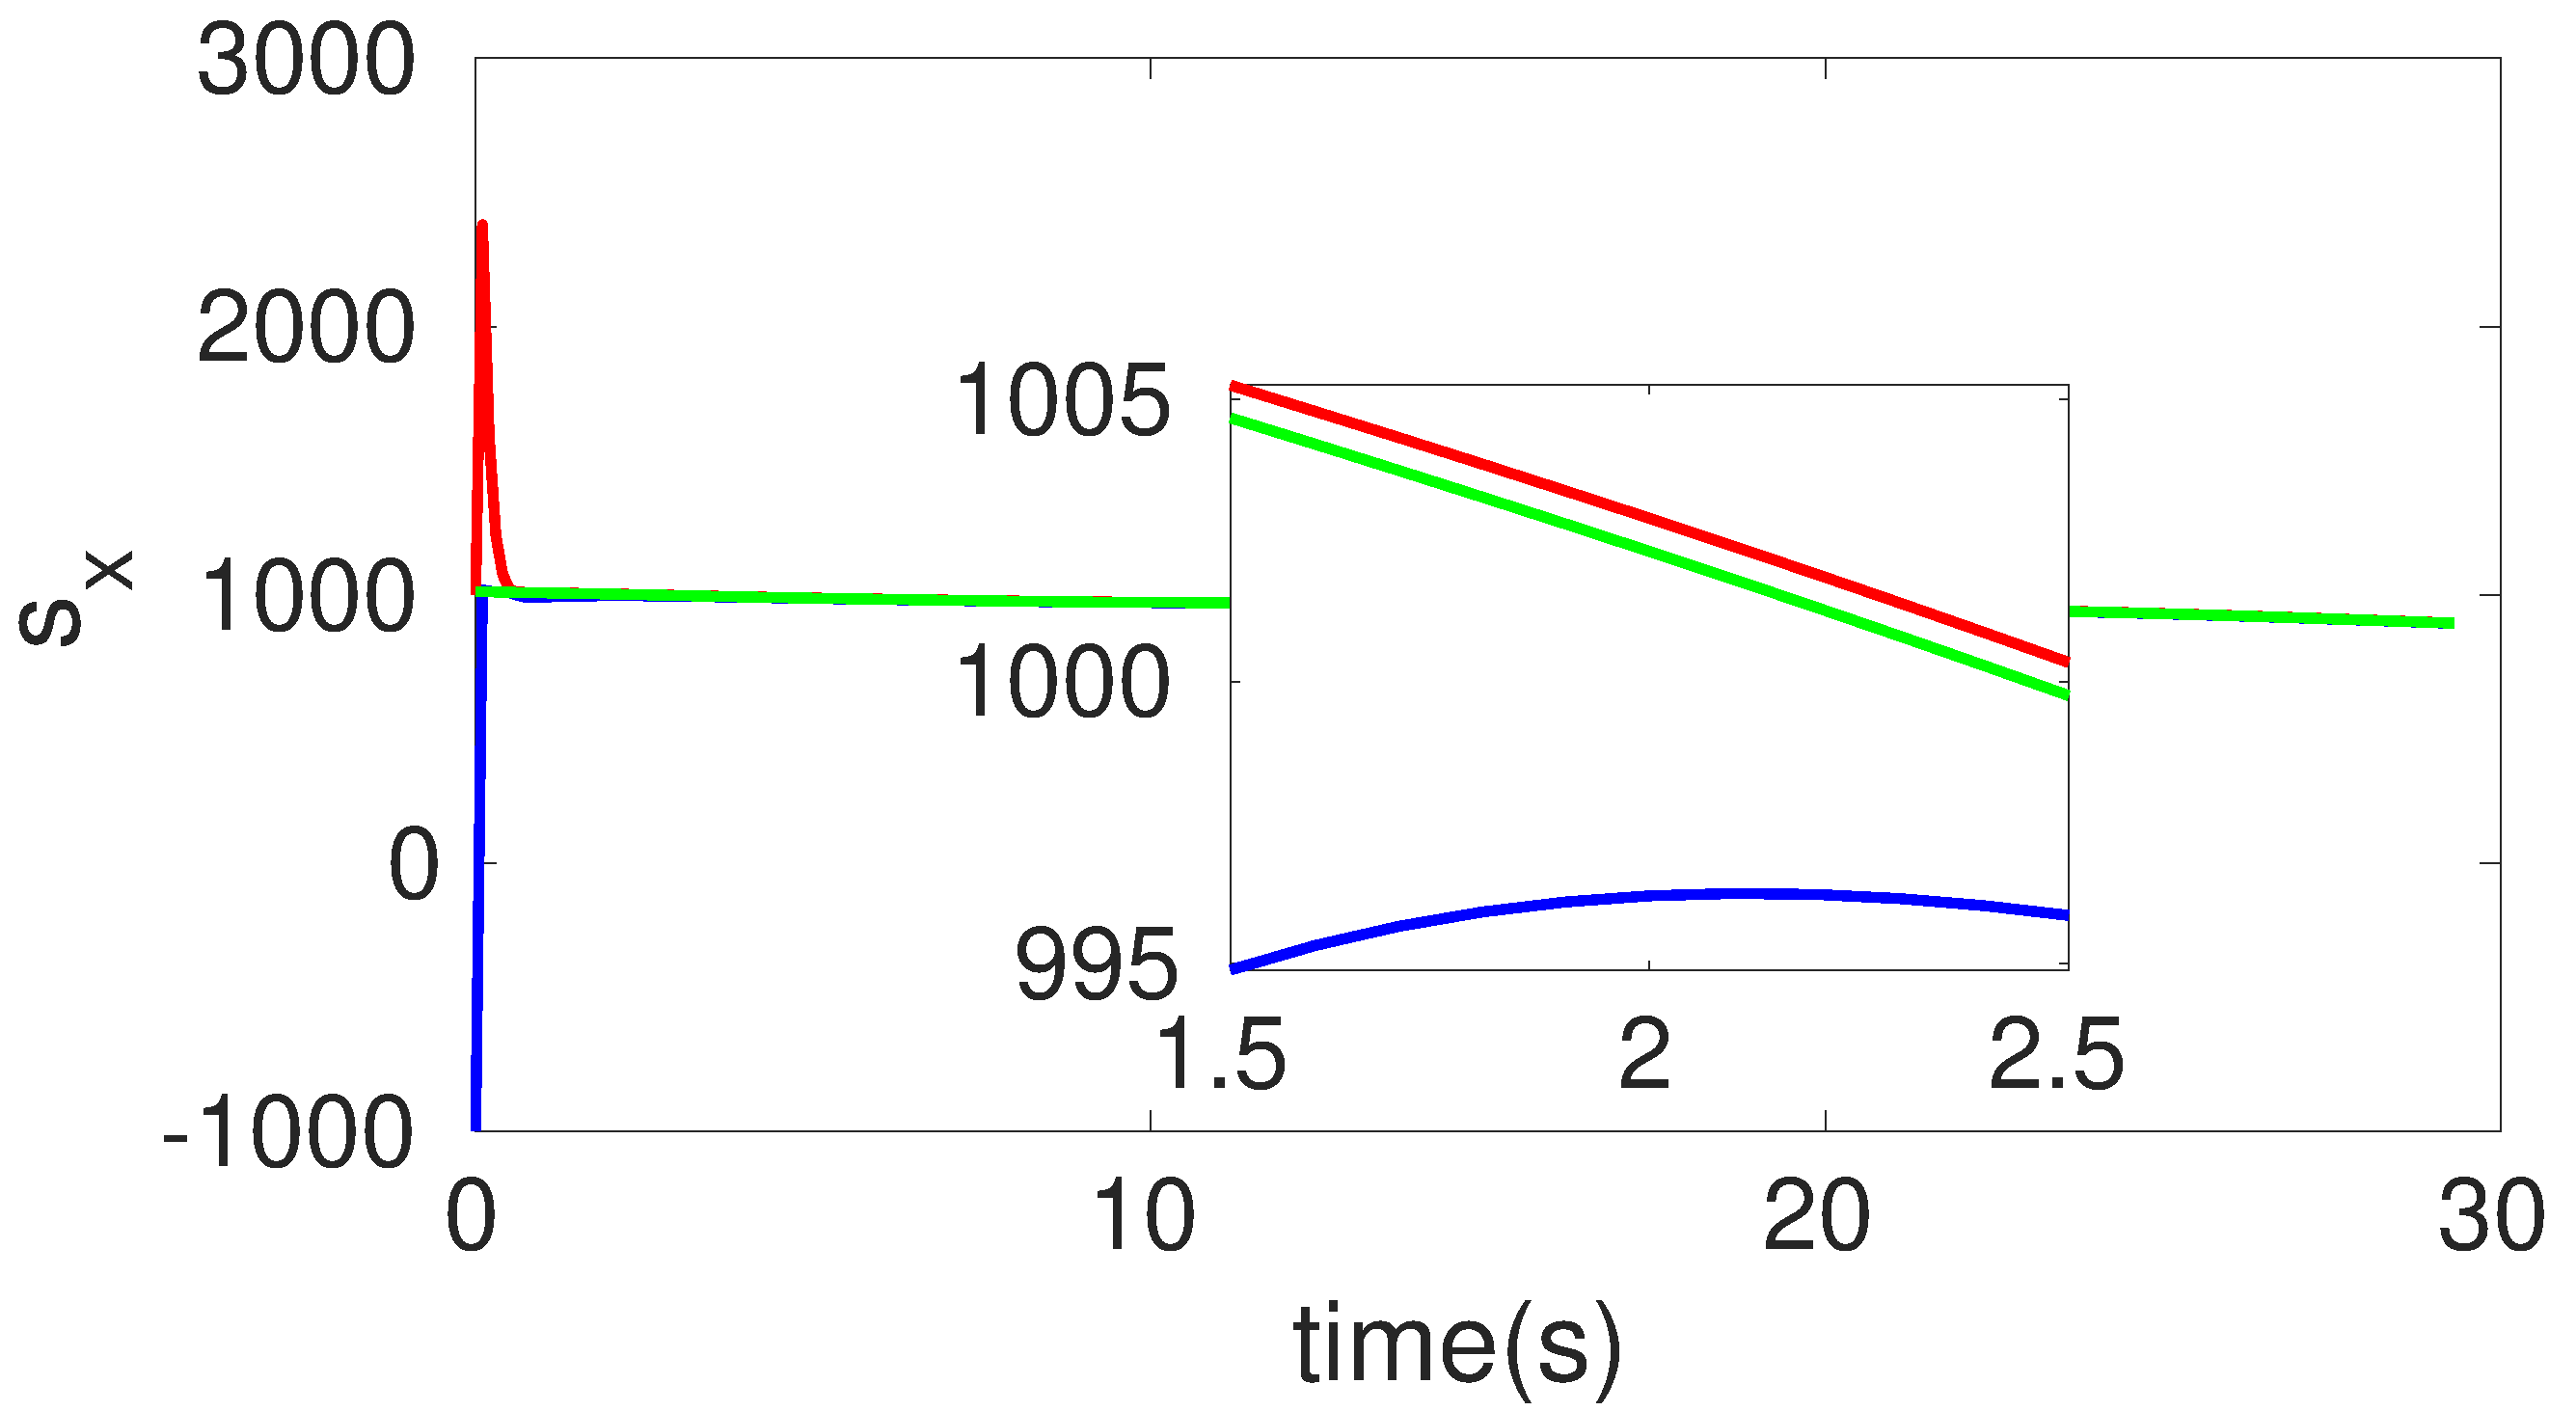
\includegraphics[width=\linewidth]{figures/HInf/s3caHInfs_x}
\end{subfigure}
\begin{subfigure}{.5\linewidth}
\centering
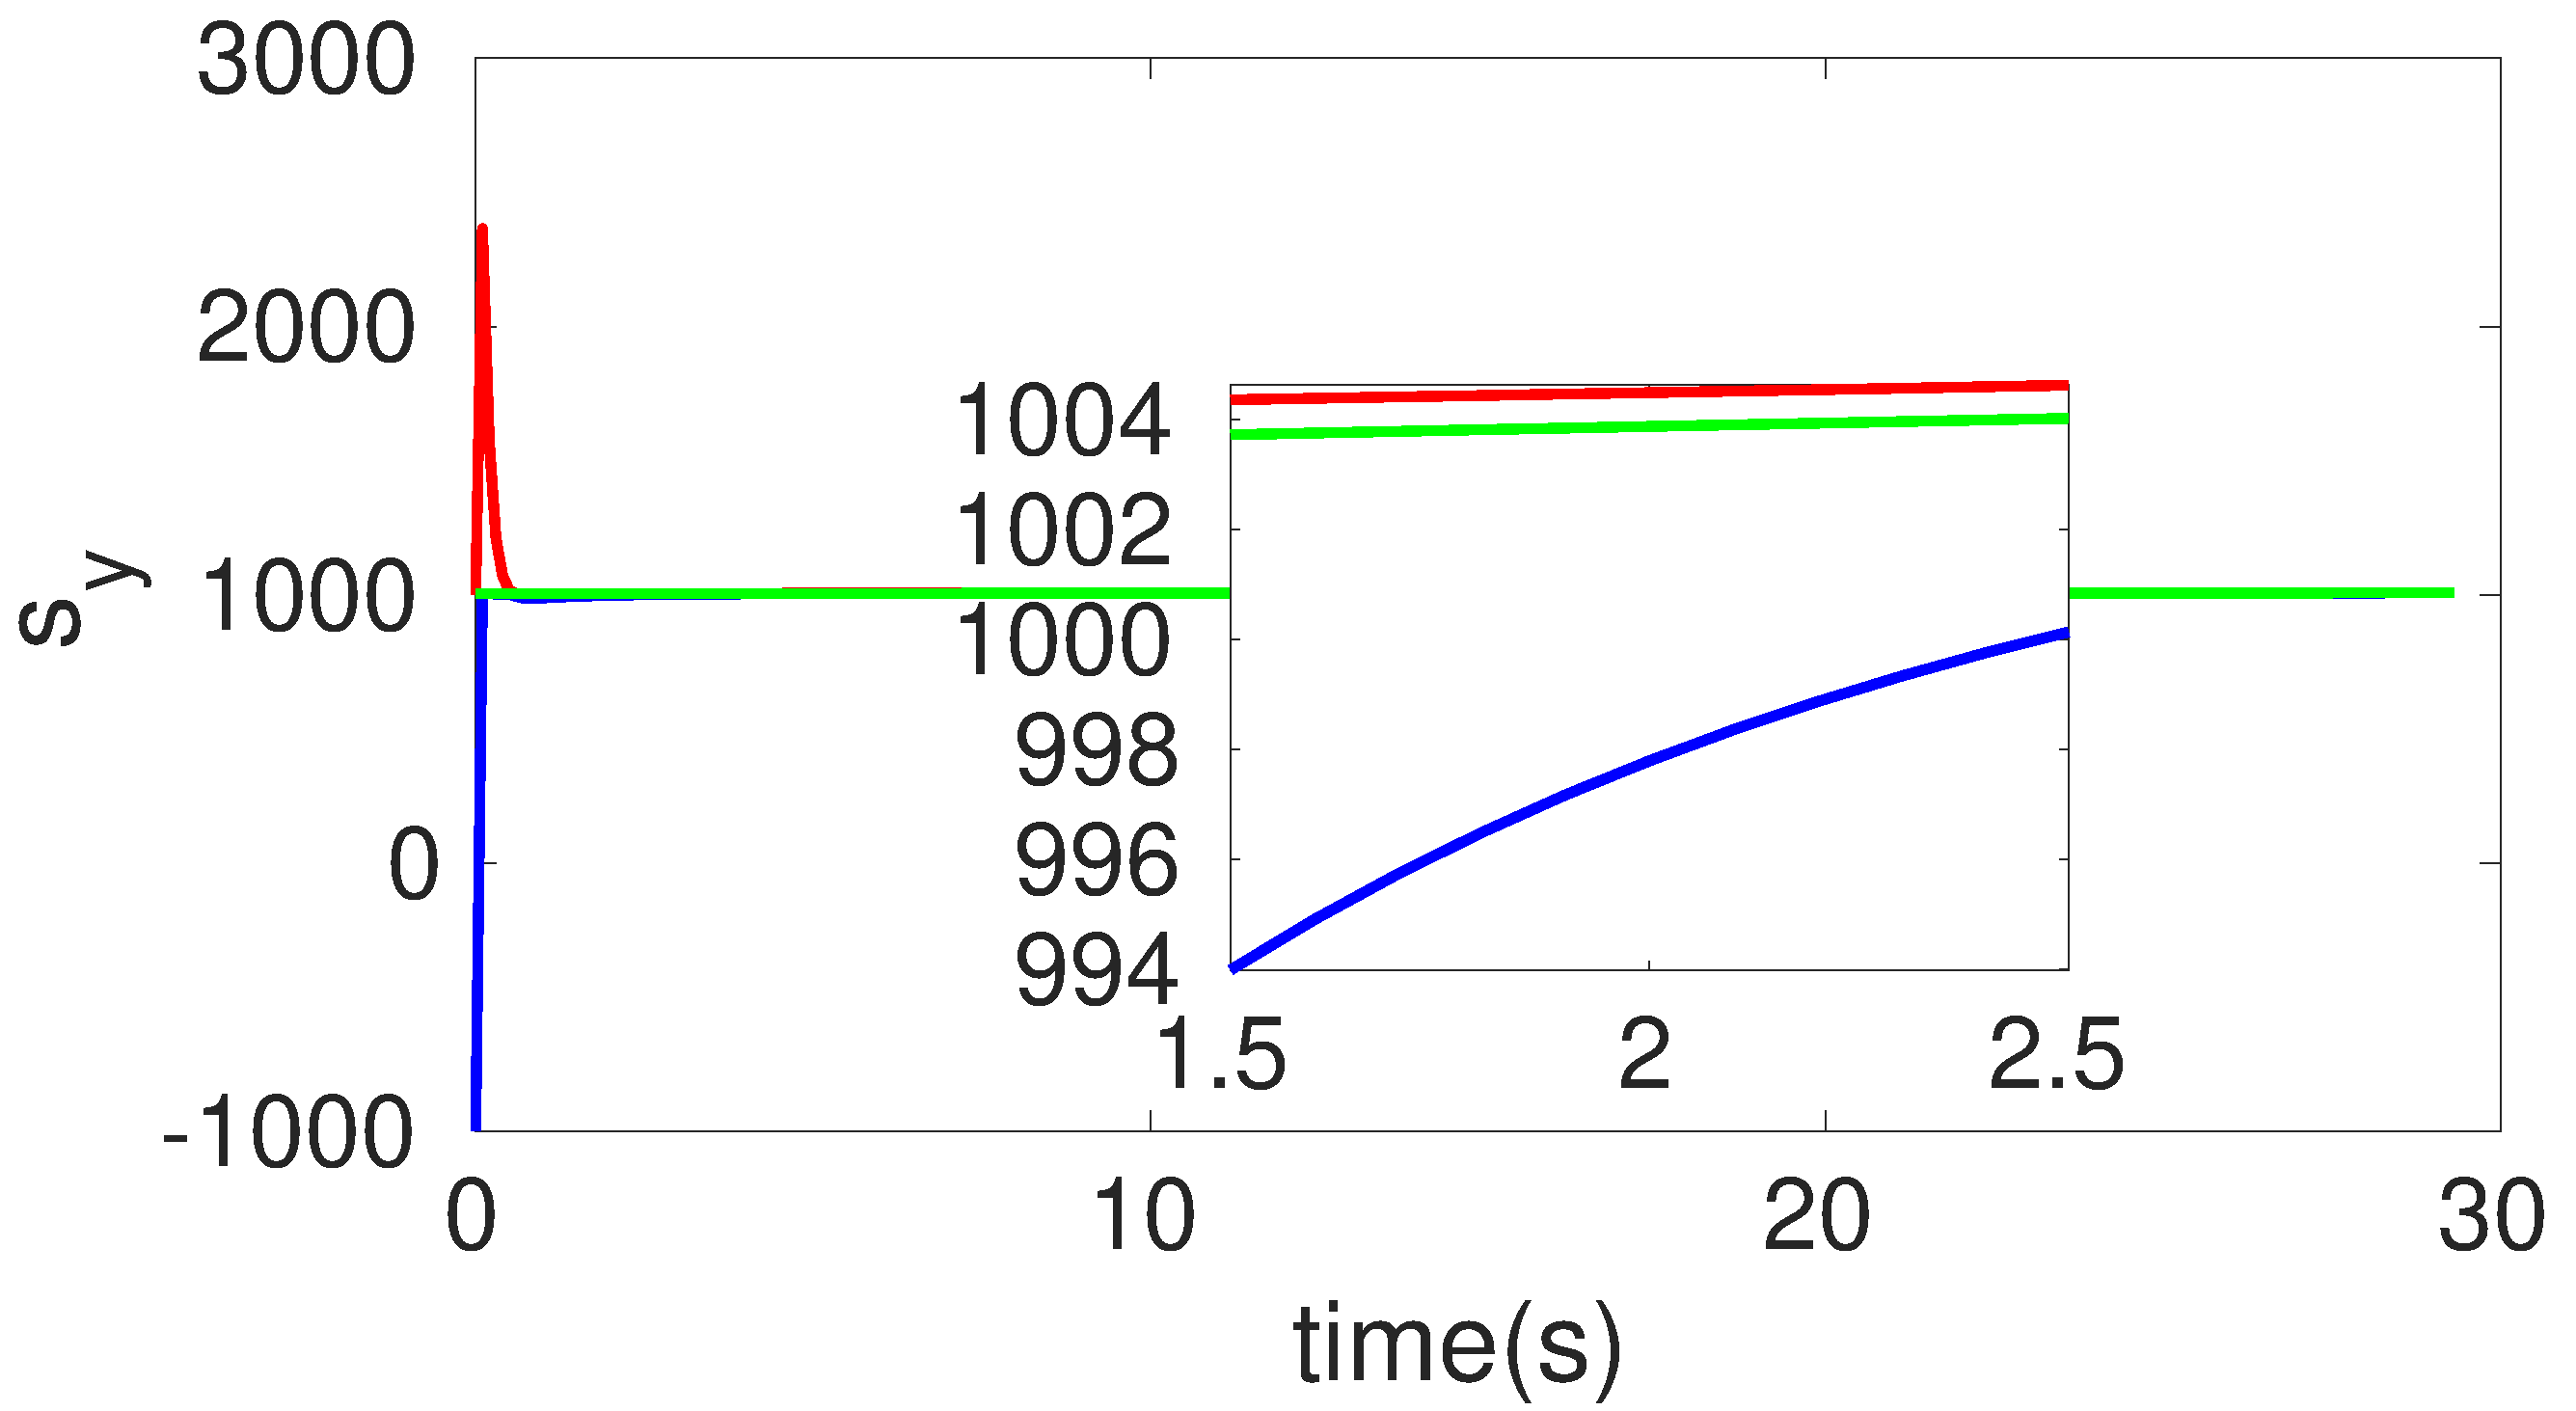
\includegraphics[width=\linewidth]{figures/HInf/s3caHInfs_y}
\end{subfigure}
\begin{subfigure}{.5\linewidth}
\centering
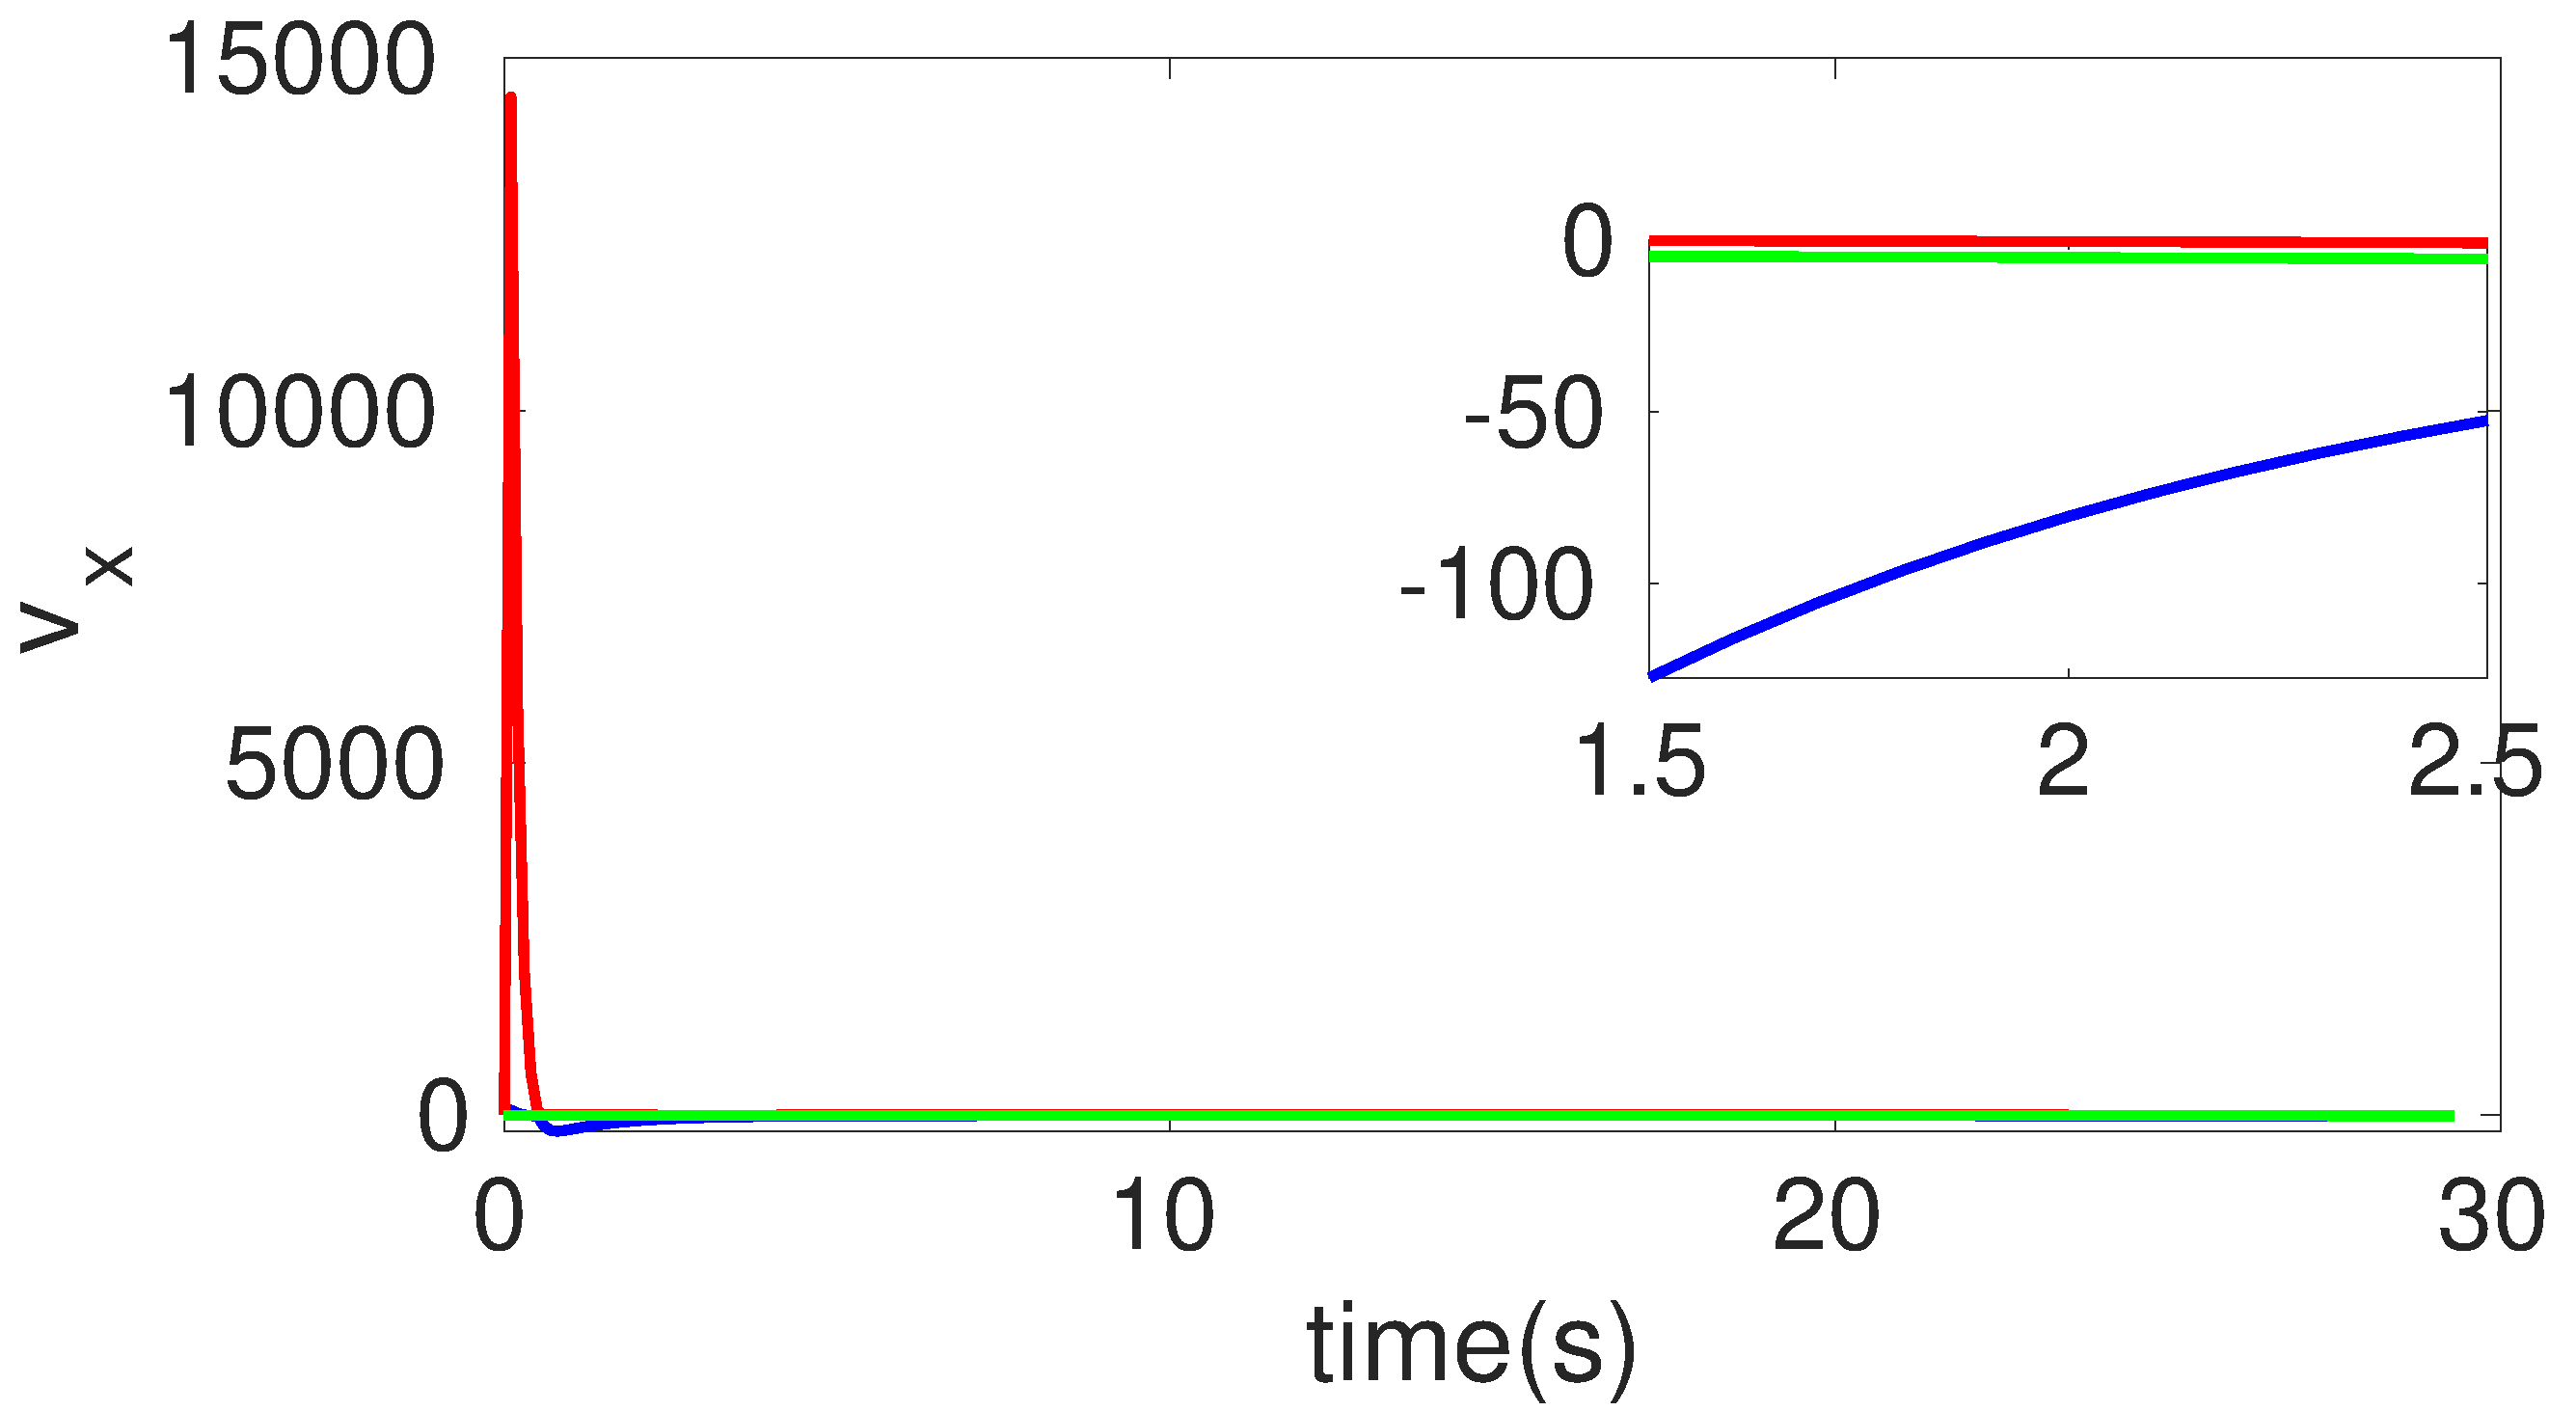
\includegraphics[width=\linewidth]{figures/HInf/s3caHInfv_x}
\end{subfigure}
\begin{subfigure}{.5\linewidth}
\centering
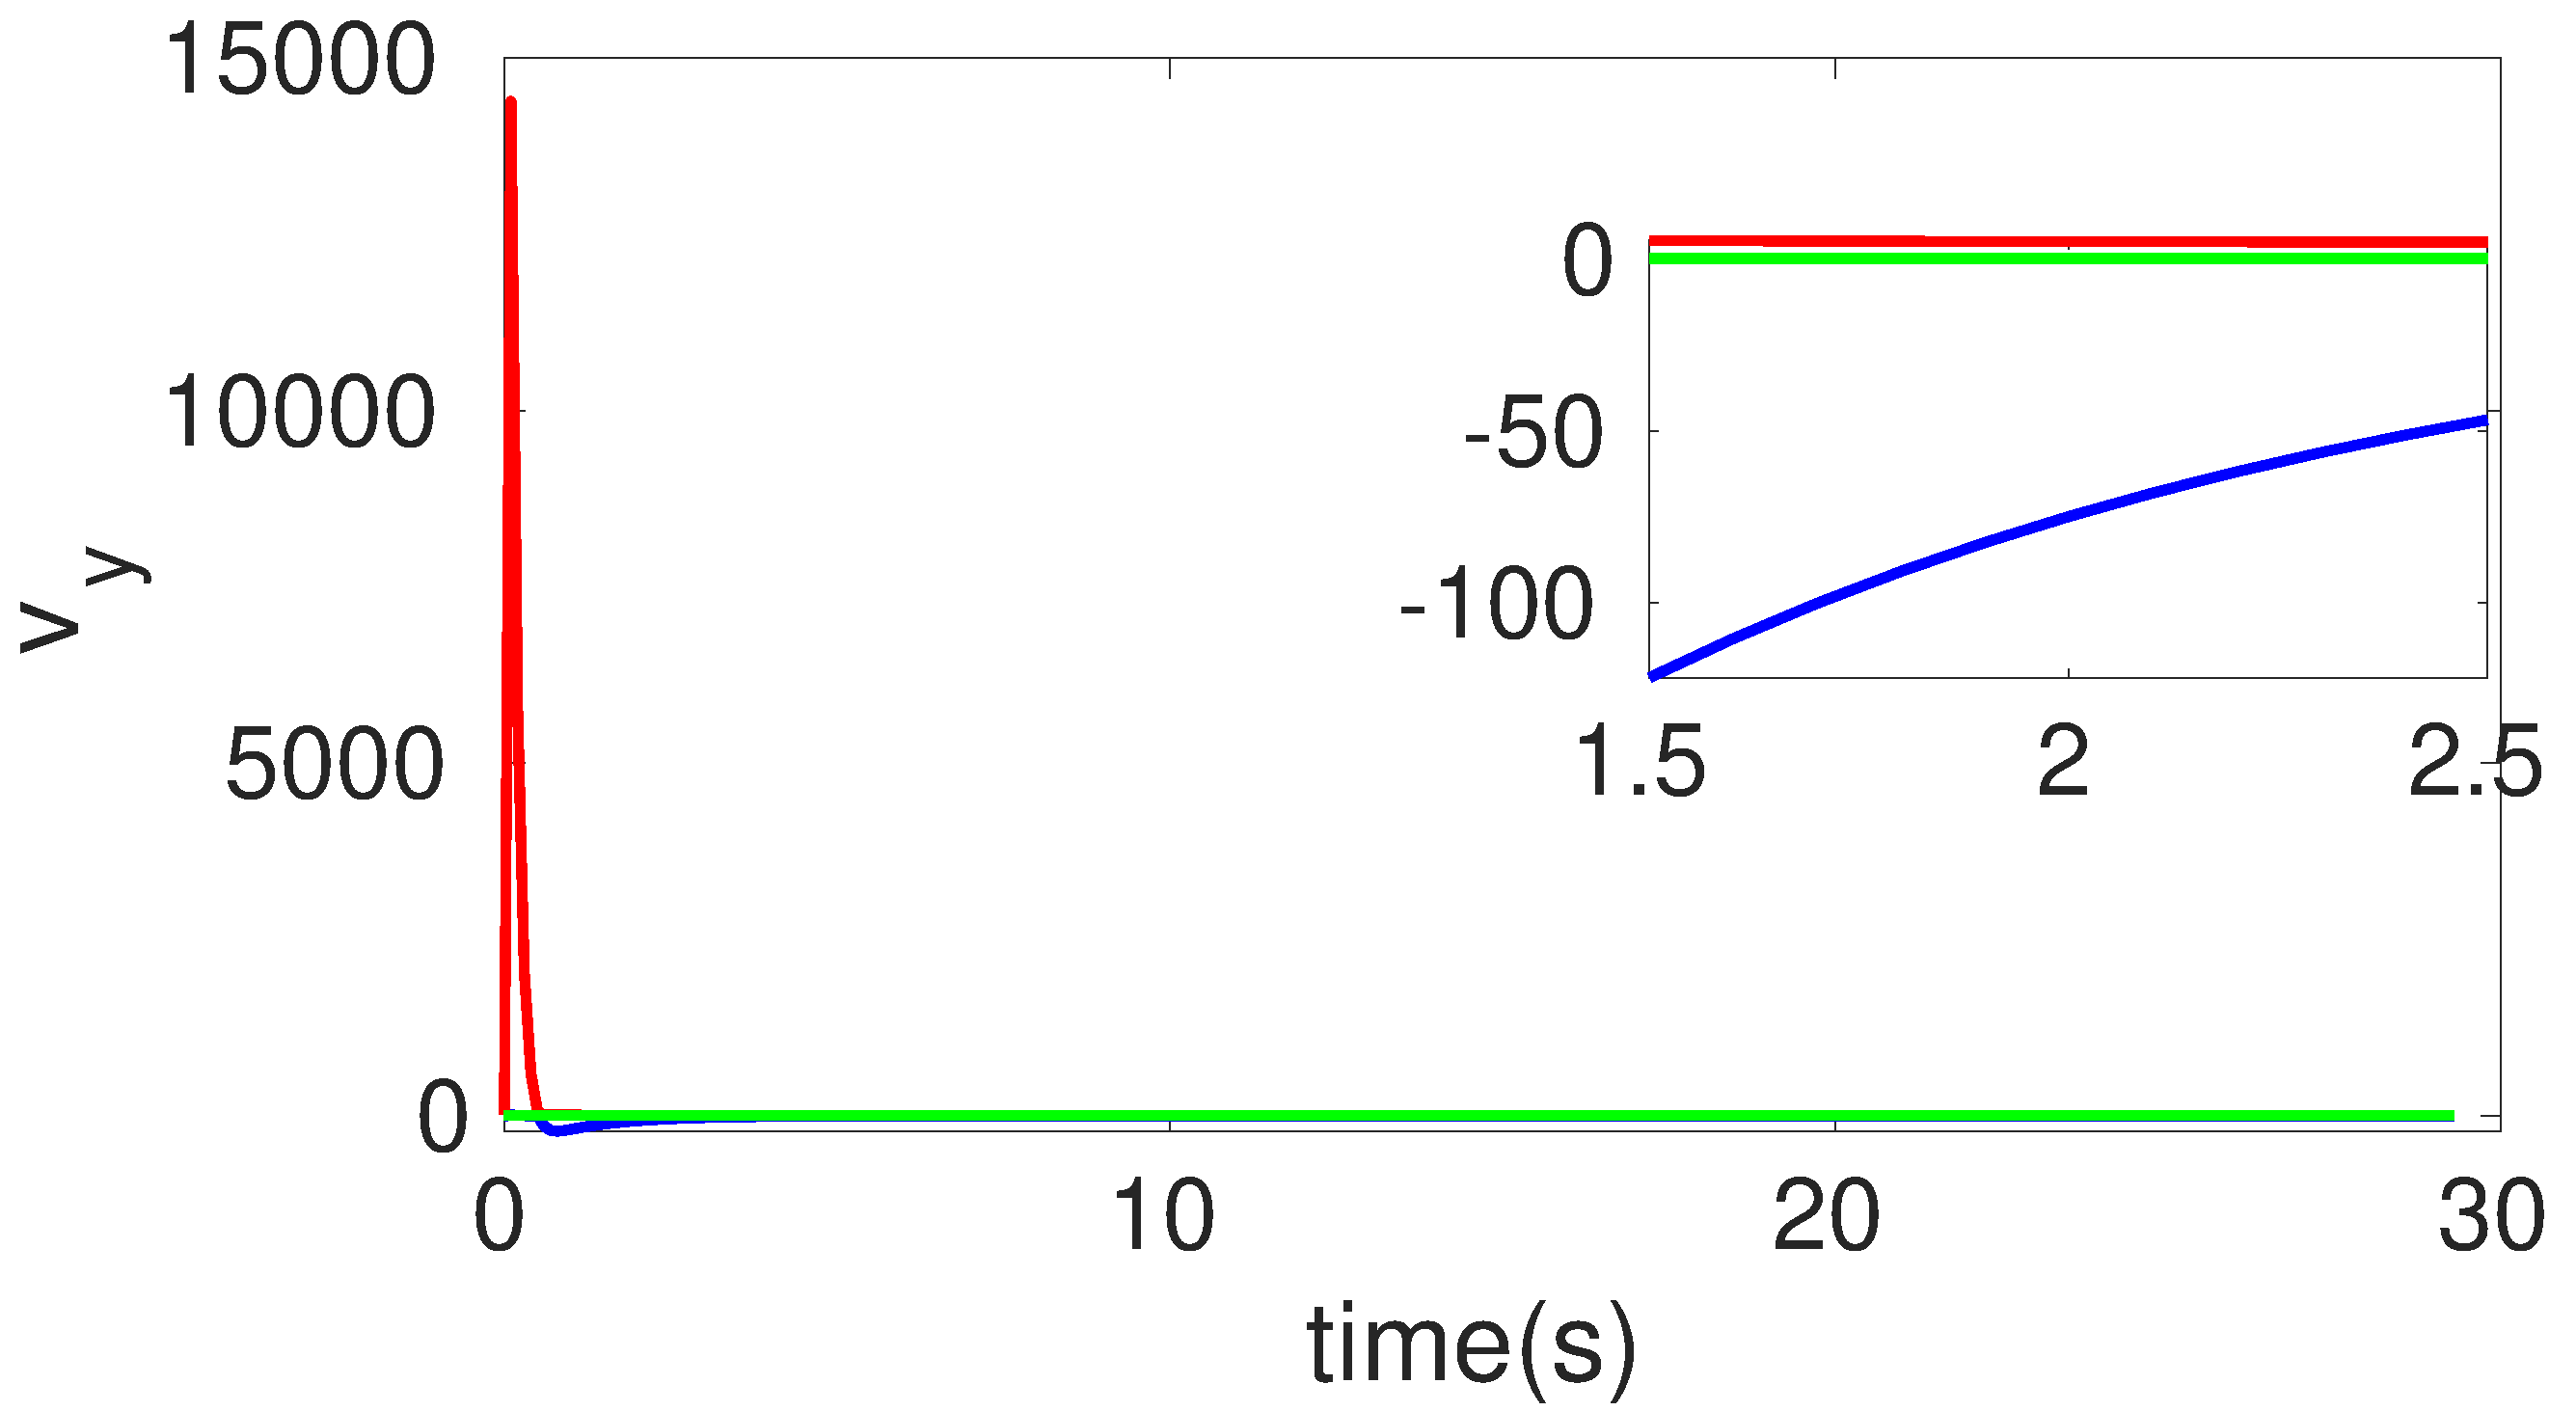
\includegraphics[width=\linewidth]{figures/HInf/s3caHInfv_y}
\end{subfigure}
\begin{subfigure}{.5\linewidth}
\centering
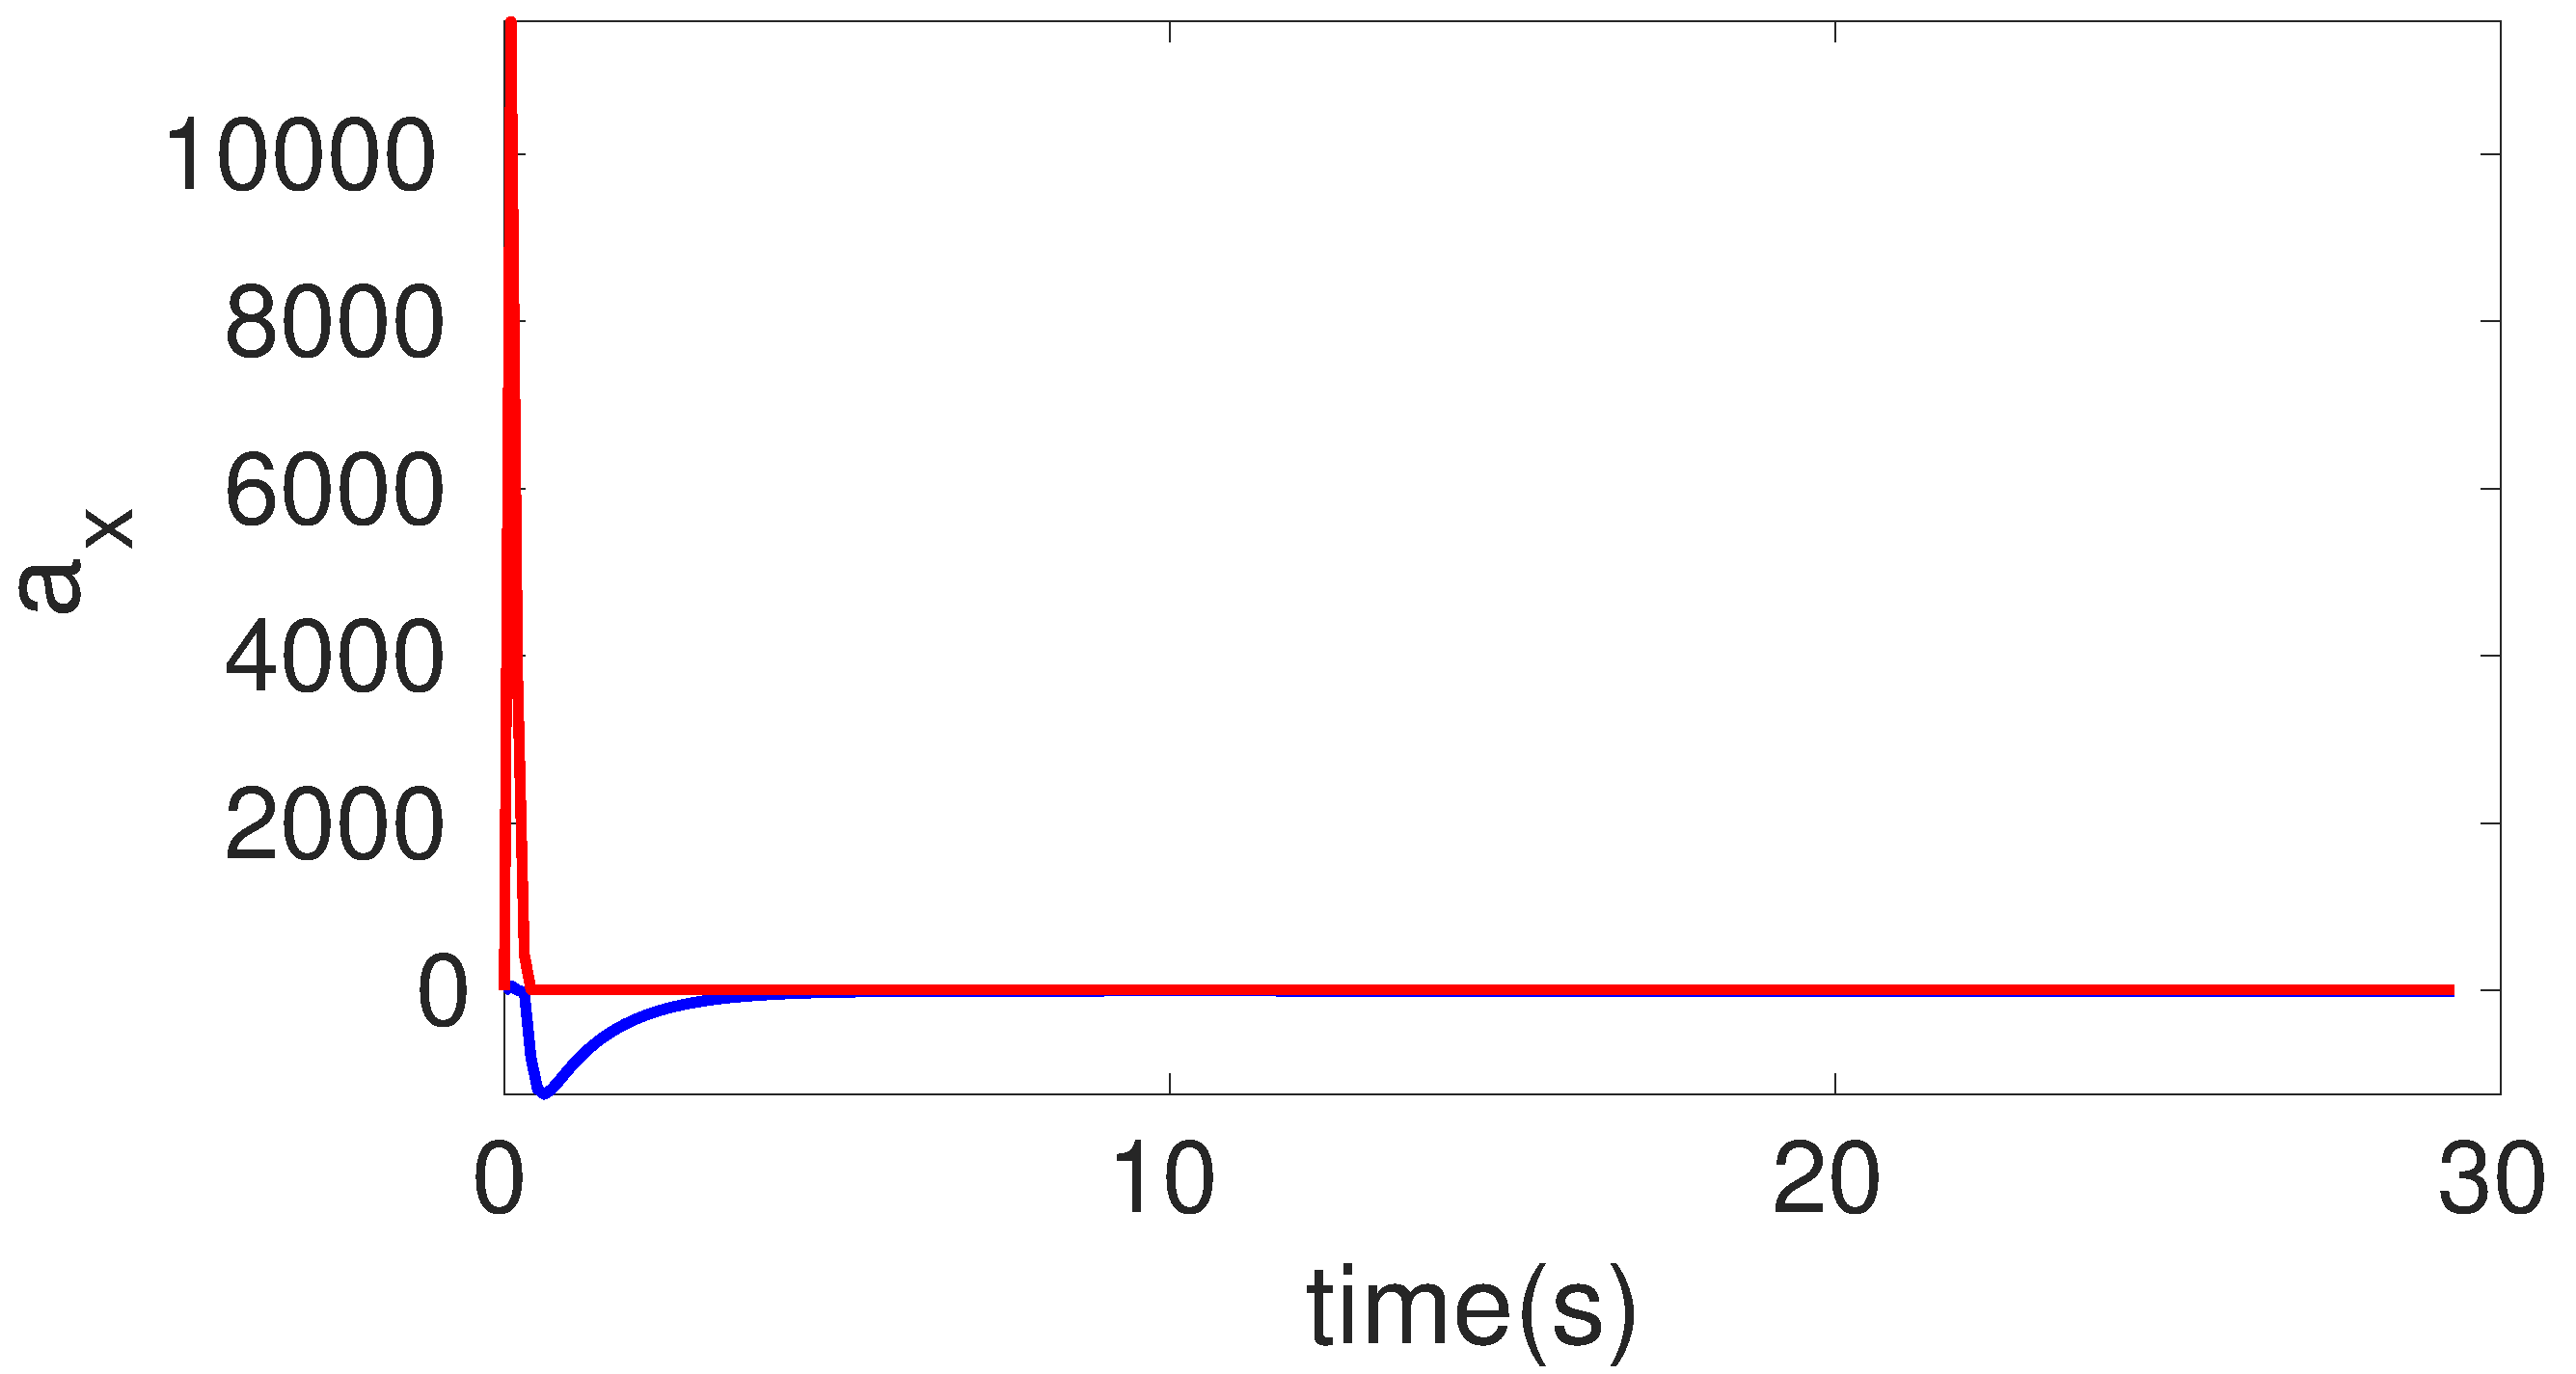
\includegraphics[width=\linewidth]{figures/HInf/s3caHInfa_x}
\end{subfigure}
\begin{subfigure}{.5\linewidth}
\centering
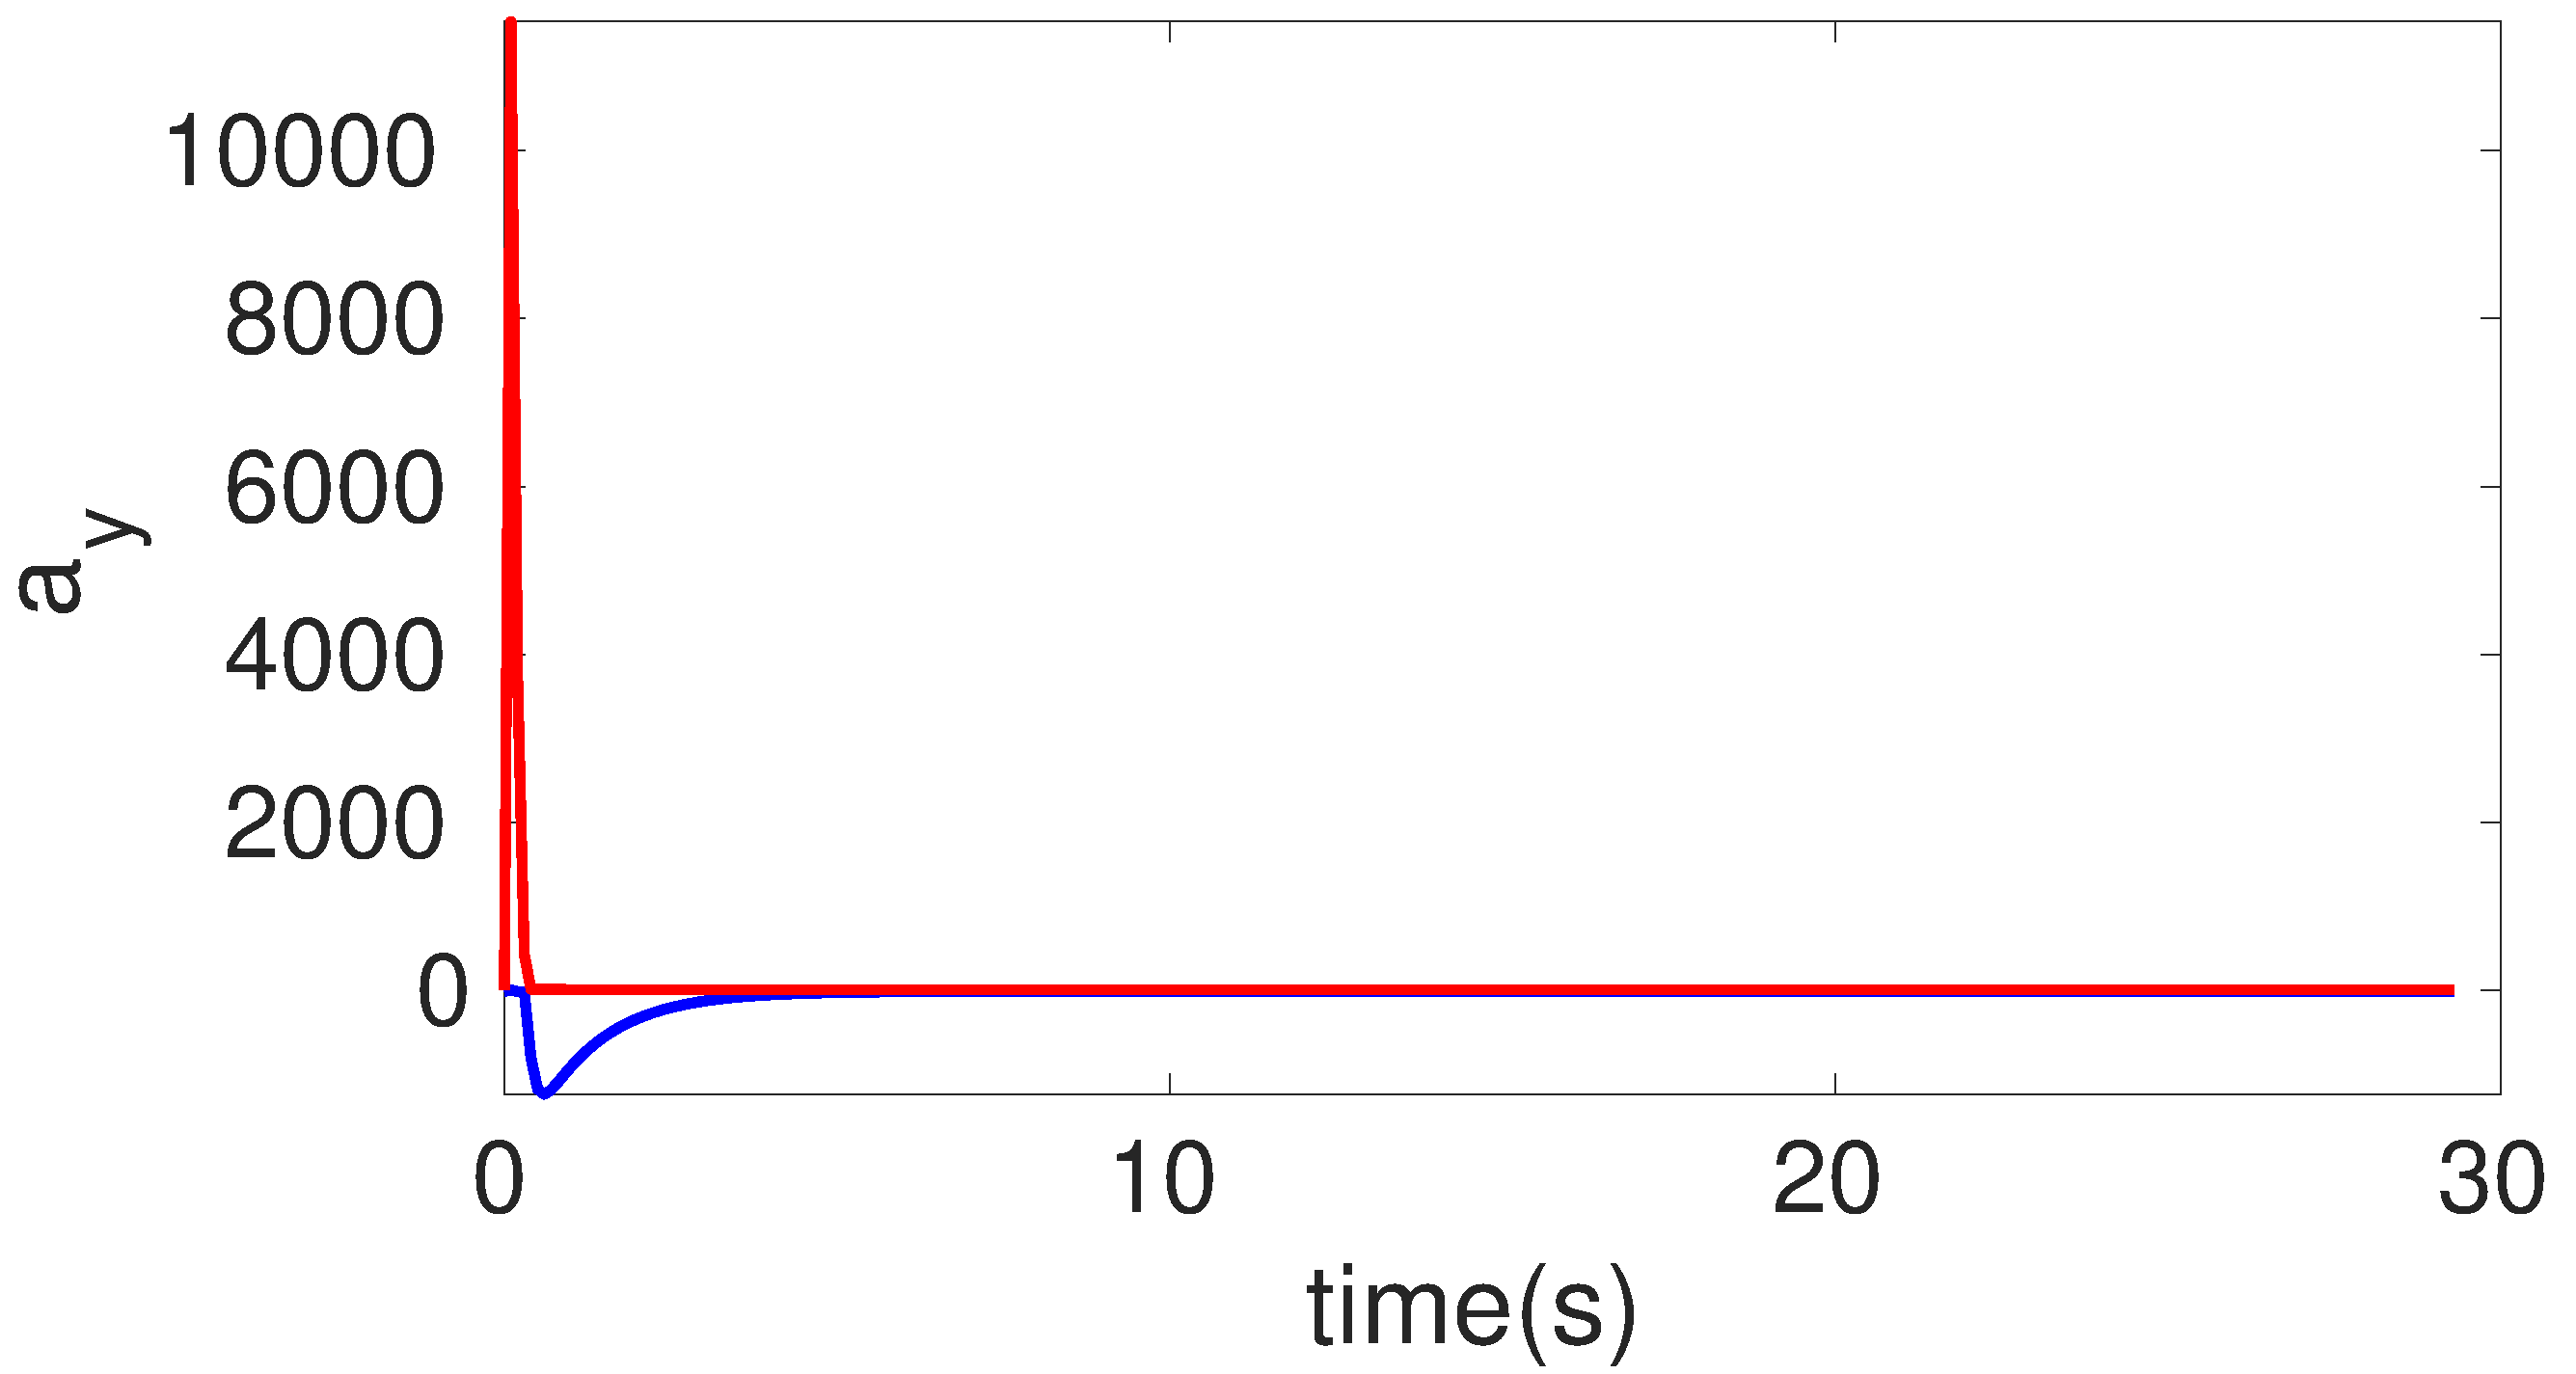
\includegraphics[width=\linewidth]{figures/HInf/s3caHInfa_y}
\end{subfigure}
\caption{Estimation using the H-$\infty$-based interval observer and the constant acceleration model}
\end{figure}

\begin{figure}[!h]
\hspace*{\fill} \includegraphics[scale=0.8]{figures/legend}\\\\
\begin{subfigure}{.5\linewidth}
\centering
\includegraphics[width=\linewidth]{figures/HInf/s3pmHInfs_x}
\end{subfigure}
\begin{subfigure}{.5\linewidth}
\centering
\includegraphics[width=\linewidth]{figures/HInf/s3pmHInfs_x}
\end{subfigure}
\begin{subfigure}{.5\linewidth}
\centering
\includegraphics[width=\linewidth]{figures/HInf/s3pmHInfv_x}
\end{subfigure}
\begin{subfigure}{.5\linewidth}
\centering
\includegraphics[width=\linewidth]{figures/HInf/s3pmHInfv_y}
\end{subfigure}
\begin{subfigure}{.5\linewidth}
\centering
\includegraphics[width=\linewidth]{figures/HInf/s3pmHInfa_x}
\end{subfigure}
\begin{subfigure}{.5\linewidth}
\centering
\includegraphics[width=\linewidth]{figures/HInf/s3pmHInfa_y}
\end{subfigure}
\caption{Estimation using the H-$\infty$-based interval observer and the point mass model}
\end{figure}

\FloatBarrier
\section{Rate of Change of Average Bounds}\label{eresult:rate}
This section demonstrates how the average bounds of estimation for approximately 9,767 entities change over time. These 9,767 entities are chosen because they have data of appropriate length for comparison.
\begin{figure}[!h]
\hspace*{\fill} \includegraphics[scale=0.8]{figures/ratelegend}\\\\
\begin{subfigure}{.5\linewidth}
\centering
\includegraphics[width=\linewidth]{figures/BoundChange/CV/cv_bound_changes_x}
\end{subfigure}
\begin{subfigure}{.5\linewidth}
\centering
\includegraphics[width=\linewidth]{figures/BoundChange/CV/cv_bound_changes_y}
\end{subfigure}
\begin{subfigure}{.5\linewidth}
\centering
\includegraphics[width=\linewidth]{figures/BoundChange/CV/cv_bound_changev_x}
\end{subfigure}
\begin{subfigure}{.5\linewidth}
\centering
\includegraphics[width=\linewidth]{figures/BoundChange/CV/cv_bound_changev_y}
\end{subfigure}
\caption{Rate of change of average bounds using the constant velocity model}
\end{figure}

\begin{figure}[!h]
\hspace*{\fill} \includegraphics[scale=0.8]{figures/ratelegend}\\\\
\begin{subfigure}{.5\linewidth}
\centering
\includegraphics[width=\linewidth]{figures/BoundChange/CA/ca_bound_changes_x}
\end{subfigure}
\begin{subfigure}{.5\linewidth}
\centering
\includegraphics[width=\linewidth]{figures/BoundChange/CA/ca_bound_changes_y}
\end{subfigure}
\begin{subfigure}{.5\linewidth}
\centering
\includegraphics[width=\linewidth]{figures/BoundChange/CA/ca_bound_changev_x}
\end{subfigure}
\begin{subfigure}{.5\linewidth}
\centering
\includegraphics[width=\linewidth]{figures/BoundChange/CA/ca_bound_changev_y}
\end{subfigure}
\begin{subfigure}{.5\linewidth}
\centering
\includegraphics[width=\linewidth]{figures/BoundChange/CA/ca_bound_changea_x}
\end{subfigure}
\begin{subfigure}{.5\linewidth}
\centering
\includegraphics[width=\linewidth]{figures/BoundChange/CA/ca_bound_changea_y}
\end{subfigure}
\caption{Rate of change of average bounds using the constant acceleration model}
\end{figure}

\begin{figure}[!h]
\hspace*{\fill} \includegraphics[scale=0.8]{figures/ratelegend}\\\\
\begin{subfigure}{.5\linewidth}
\centering
\includegraphics[width=\linewidth]{figures/BoundChange/PM/pm_bound_changes_x}
\end{subfigure}
\begin{subfigure}{.5\linewidth}
\centering
\includegraphics[width=\linewidth]{figures/BoundChange/PM/pm_bound_changes_y}
\end{subfigure}
\begin{subfigure}{.5\linewidth}
\centering
\includegraphics[width=\linewidth]{figures/BoundChange/PM/pm_bound_changev_x}
\end{subfigure}
\begin{subfigure}{.5\linewidth}
\centering
\includegraphics[width=\linewidth]{figures/BoundChange/PM/pm_bound_changev_y}
\end{subfigure}
\begin{subfigure}{.5\linewidth}
\centering
\includegraphics[width=\linewidth]{figures/BoundChange/PM/pm_bound_changea_x}
\end{subfigure}
\begin{subfigure}{.5\linewidth}
\centering
\includegraphics[width=\linewidth]{figures/BoundChange/PM/pm_bound_changea_y}
\end{subfigure}
\caption{Rate of change of average bounds using the point-mass model}
\end{figure}
\pagebreak
